\documentclass[10pt,openright,twoside]{book}
% LK: added twoside, headheight, headsep
\usepackage[paperwidth=142mm,paperheight=197mm,top=24mm,bottom=22mm,inner=18mm,outer=22mm]{geometry}
\usepackage[cam,a4,center]{crop}
% \usepackage[utf8]{inputenc}
\usepackage{graphicx}

%% LK: \usepackage[magyar]{babel}
\usepackage{polyglossia}
\setdefaultlanguage{magyar}
\usepackage{aref}
\usepackage{needspace}
\usepackage{setspace}
\widowpenalty=300
\clubpenalty=300
\setlength\parskip{0pt}
\raggedbottom
\widowpenalty=10000
\clubpenalty=10000

\usepackage{leading}
\leading{13pt}


%% :LK

\usepackage{verbatim}
\usepackage{booktabs}
%\usepackage[colorinlistoftodos,prependcaption,textsize=tiny]{todonotes}

\usepackage{fontspec}

%% LK:
\setmainfont[Mapping=tex-text]{Minion Pro}
\newfontfamily\submainfont[Mapping=tex-text,Scale=0.9]{Minion Pro}
\newfontfamily\chapterfont[Mapping=tex-text,Scale=2.0]{Myriad Pro Bold}
\newfontfamily\sectionfont[Mapping=tex-text,Scale=1.2]{Myriad Pro}
\newfontfamily\subsectionfont[Mapping=tex-text]{Myriad Pro}
\newfontfamily\subsubsectionfont[Mapping=tex-text]{Myriad Pro Bold}
\newfontfamily\paragraphfont[Mapping=tex-text,Scale=0.9]{Minion Pro Bold}
%% :LK
\usepackage[raggedright]{titlesec}
%% LK:
\titleformat{\chapter}[display]%
            {\chapterfont}{\thechapter. fejezet}%
            {0.5 ex}{\vspace{1ex}}
\titleformat{\section}{\sectionfont}{\thesection.}{0.5em}{}
\titleformat{\subsection}{\subsectionfont}{}{the}{\MakeUppercase}
\titleformat{\subsubsection}
{\subsubsectionfont}{}{}{}
\titleformat{\paragraph}[runin]{\paragraphfont}{}{}{}
%% chaptert romai szamokkal
\renewcommand{\thechapter}{\Roman{chapter}}
\renewcommand*\thesection{\arabic{section}}
%% tartalomjegyzek
%% innen masoltam https://tex.stackexchange.com/questions/380933/toc-with-auto-spacing-for-roman-enumeration
\usepackage[rightlabels]{titletoc}
\contentsmargin{1.5em}
\titlecontents{chapter}
[2em] %
{\bigskip}
{\contentslabel[\thecontentslabel.]{2em}\hspace{0.333em}}%\thecontentslabel
{\hspace*{-2em}}
{\hfill\contentspage}[\smallskip]%\hfill

\titlecontents{section}% <section>
[2.35em]% <left>
{\small\contentsmargin{1.5em}}% <above-code>
{\thecontentslabel.\hspace{3pt}}% <numbered-entry-format>; you could also use {\thecontentslabel. } to show the numbers
{}% <numberless-entry-format>
{\enspace\titlerule*[0.5pc]{.}~\contentspage}% <filler-page-format>

\titlecontents*{subsection}% <section>
[3.23em]% <left>
{\footnotesize\contentsmargin{0em}}% <above-code>
{\thecontentslabel. \hspace{3pt}}% <numbered-entry-format>; you could also use {\thecontentslabel. } to show the numbers
{}% <numberless-entry-format>
{}% <filler-page-format>
[ --- \ ]% <separator>
[]% <end>
%% tartalomjegyzek vege

%% subsection alatt nincs mar szamozas es nem is kerul a tartalomjegyzekbe
%% UpperCase lesz a subsection es sima bold a subsubsection
\setcounter{secnumdepth}{1}
\setcounter{tocdepth}{1}

%% :LK
\usepackage{caption}
\DeclareCaptionLabelFormat{swappedTable}{#2. táblázat}
\captionsetup[table]{labelformat=swappedTable}
\DeclareCaptionLabelFormat{swappedFigure}{#2. ábra}
\captionsetup[figure]{labelformat=swappedFigure}
\setlength{\parskip}{0pt}
\raggedbottom
\usepackage{fancyhdr}
%% LK:
% \fancyhead[LE]{\thepage\qquad{\small\leftmark}}
% \fancyhead[RO]{{\small\leftmark}\qquad\thepage}
% \fancyhead[LO,RE]{}
\fancyhead{}                              % clear header fields
\fancyhead[RO,LE]{{\submainfont\thepage}} % right odd, left even
\fancyhead[CE]{\small\textsc{Tanulni tanulunk -- A Budapest School Modell}}
\fancyhead[CO]{\small\textsc{\leftmark}}

\pagestyle{fancy}
\renewcommand{\sectionmark}[1]{\markright{#1}}
\renewcommand{\chaptermark}[1]{\markboth{#1}{}}
%\renewcommand{\chaptermark}[1]{\markright{#1}}
%\renewcommand{\sectionmark}[1]{\markboth{#1}}
%\renewcommand{\subsectionmark}[1]{}
%% :LK
\fancyfoot{}
\renewcommand{\headrulewidth}{0pt}


\usepackage{longtable}
\usepackage{array}
\usepackage[justification=centering]{caption}
\usepackage{url}
\usepackage[nottoc,numbib]{tocbibind}
% \DeclareUnicodeCharacter{2212}{-}
% heylyseglista tablazat miatt
\usepackage{graphicx}
\usepackage{lscape}
\usepackage{natbib}


%% ezek kellenek a ketoldalas kepekhez. pdfpage berak uj oldalt
\usepackage{pdfpages}
%% ez meg baloldalt kezdi a kepet
\newcommand*\cleartoleftpage{%
  \clearpage
  \ifodd\value{page}\hbox{}\newpage\fi
}
% This package suppresses page numbers and headings from appearing on empty pages.
\usepackage{emptypage}
%% ezzel rakunk be ketoldalas kepeket. Mindig kettesevel
%% rakunk be kepeket, balra es jobbra, teljes oldalra, fejlec nelkul.
\newcommand{\ketoldaltkep}[2]{
    \cleartoleftpage
    \includepdf{#1}
    \includepdf{#2}
}

%% ez van a chapter elotti kepek
\newcommand{\chaptercover}[1]{
    \cleardoublepage
    \includepdf{#1}
}
\begin{document}
% csinalunk egy feltetelt, hogy a szovegben tudjuk, hogy kerettantervben vagyunk
% vagy a pedprogramban
\newif\ifkerettanterv
\kerettantervtrue

\title{Tanulni Tanulunk \\ A Budapest School Modell}
\author{Halácsy Péter \and Halmos Ádám}
\date{2019. augusztus}
\frontmatter
\begin{titlepage} % Suppresses headers and footers on the title page

	\centering % Centre everything on the title page
	
	\scshape % Use small caps for all text on the title page
	
  \vspace*{\baselineskip} % White space at the top of the page
  {\Large Tanulni Tanulunk}\\
  A\\
    Budapest School\\
    Modell
\end{titlepage}


   
%% copyright page
\clearpage\null\vfill
\pagestyle{empty}
\begin{minipage}[b]{0.9\textwidth}
\footnotesize\raggedright
\setlength{\parskip}{0.5\baselineskip}
Kiadja a Misulink Nonprofit Kft.\\
Felelős kiadó: Halácsy Péter \\
Felelős szerkesztő: Halmos Ádám \\
Illusztráció: Matyus Dóra és Máthé Kata (remarker.eu) \\
Olvasószerkesztő: Györke Mária \\
Műszaki szerkesztő: Halmos Mária \\
Tördelő: Kálmán László\\
Készült 2019-ben a Gyomai Kner Nyomda Zrt-ben \\
Felelős vezető Erdős Tamás  vezérigazgató \\
ISBN 978-615-00-5945-7\\
\smallskip
Ez a könyv a Creative Commons Attribution-ShareAlike 3.0 Unported (CC BY-SA 3.0) licenc szerint terjeszthető és/vagy módosítható.
\end{minipage}
\vspace*{2\baselineskip}
\cleardoublepage

%% end of copyrigth page

\newlength\longest
\cleardoublepage
\thispagestyle{empty}
\null\vfill
{\centering
\parbox{0.8\textwidth} {%
    \raggedright{\large\itshape%
    Ha egy gyerek nem érett meg az algebrára, hiába kínozzuk vele,  
    ha meg igen: nem kell hosszú évekig kanalas orvosságként adagolni neki. \\
    Az osztályban oktatás természete szerint idomítással gyötri az éretlent 
    és kedvét szegi az érettnek. \\
    A ,,csoportban'' olyan gyerekek kerülnek össze, akik egy-egy téren 
    nagyjából egyformán érettek. S addig rágják az előttük lévő anyagot, amíg erejükből futja. \ldots Két-három hónap múlva a résztvevő új csoportba kerül, s más képességét edzi tovább.

        \par\bigskip
    }
    \raggedleft\Large\MakeUppercase{Németh László, 1945}\par%
    \raggedleft\normalsize{író (eredetileg fogorvos)}\par%
}\par%
}
\vfill\vfill
\cleardoublepage
\thispagestyle{empty}
\null\vfill
{\centering
\parbox{0.8\textwidth} {%
    \raggedright{\large\itshape%
    Experiments show that children in unsupervised groups, using the internet, are capable of answering questions many years ahead of the material they’re learning in school. In fact, they seem to enjoy the absence of adult supervision, and they are very confident of finding the right answer.

        \par\bigskip
    }
    \raggedleft\Large\MakeUppercase{Sugata Mitra, 2015}\par%
    \raggedleft\normalsize{oktatáskutató}\par%
}\par%
}

\vfill\vfill
\clearpage



\begin{titlepage} % Suppresses headers and footers on the title page

	\centering % Centre everything on the title page
	
	\scshape % Use small caps for all text on the title page
	
	\vspace*{\baselineskip} % White space at the top of the page
	
		%------------------------------------------------
	%	Title
	%------------------------------------------------
	
	\rule{\textwidth}{1.6pt}\vspace*{-\baselineskip}\vspace*{2pt} % Thick horizontal rule
	\rule{\textwidth}{0.4pt} % Thin horizontal rule
	
	\vspace{0.75\baselineskip} % Whitespace above the title
	
	{\LARGE Tanulni Tanulunk\\} % Title
	
	\vspace{0.75\baselineskip} % Whitespace below the title
	
	\rule{\textwidth}{0.4pt}\vspace*{-\baselineskip}\vspace{3.2pt} % Thin horizontal rule
	\rule{\textwidth}{1.6pt} % Thick horizontal rule
	
	\vspace{2\baselineskip} % Whitespace after the title block
	
	
	%------------------------------------------------
	%	Subtitle
	%------------------------------------------------
	
    %%Hol, milyen módon, kitől és mit tanulhat \\
    %%egy Budapest Schoolba járó gyerek
    A\\
    Budapest School\\
    Modell
    % Subtitle or further description
	
	\vspace*{3\baselineskip} % Whitespace under the subtitle
	
	%------------------------------------------------
	%	Editor(s)
	%------------------------------------------------
	
	Szerkesztette
	
	\vspace{0.5\baselineskip} % Whitespace before the editors
	
	{\scshape\Large Halácsy Péter \\ Halmos Ádám \\} % Editor list
	
	\vspace{0.5\baselineskip} % Whitespace below the editor list
	
	\textit{Budapest School \\ Általános Iskola és Gimnázium} % Editor affiliation
	
	\vfill % Whitespace between editor names and publisher logo
	
	%------------------------------------------------
	%	Publisher
	%------------------------------------------------
	
	
\includegraphics[width=2cm]{logo}
	
	\vspace{0.3\baselineskip} % Whitespace under the publisher logo
	
	2019 % Publication year
	
	

\end{titlepage}
%\pagestyle{empty}

\noindent
\textit{Prof. Dr. Kásler Miklós Miniszter Úr \\
      részére}
\vspace{0.75cm}

\noindent
\textbf{tárgy}: felülvizsgálat

\noindent
\textbf{iktatószám}: 14259-7/2019/KÖZNEVTART
\vspace{0.75cm}

\noindent
Tisztelt Miniszter Úr!
\vspace{0.75cm}

\noindent
A MiSulink Nonprofit Korlátolt Felelősségű Társaság (székhely: 1118 Budapest, Breznó köz 8., Cg. 01-09-209663), mint a Budapest School Általános Iskola és Gimnázium (nyilvántartási szám: 702.) fenntartója azzal a tiszteletteljes kéréssel fordulunk Önhöz, hogy a mellékelt kerettanterv-módosítást jóváhagyni szíveskedjen!

Tisztelt Miniszter Úr nevében eljárva Dr. Maruzsa Zoltán Helyettes Államtitkár Úr 2019. április 30. napján \texttt{14259-7/2019/KOZNEVTART} számon jóváhagyta a \textit{Budapest School Kerettanterv} elnevezésű kerettantervünket.

A 2019. július 26. napjától hatályos a köznevelési törvényt módosító 2019. évi LXX.  sz. törvény. A módosító törvény következtében az Nkt. 9. § (9a) bekezdéssel egészült ki. Ennek értelmében:

\begin{quote}
,,(9a) A (9) bekezdés alkalmazása során az alternatív kerettanterv csak akkor hagyható jóvá, ha megfelel a következő szempontoknak: \\
a) a Nat-ban meghatározott tananyag tartalmakat tanévenként két félévre bontva kell megjeleníteni a kerettantervekben, összhangban a tanulók félévenkénti értékelésével, \\
b) a Nat-ban foglalt műveltségi területek adaptálása során az iskolák közötti átjárhatóság és a továbbtanulás biztosítása érdekében az alternatív kerettanterv tantárgyi struktúrája legfeljebb harminc százalékban térhet el az oktatásért felelős miniszter által kiadott kerettantervben foglalt tantárgyi struktúrától.” \\
\end{quote}

A fenti előírásoknak a jelen kérelmünkhöz mellékelt módosított, egységes szerkezetbe foglalt kerettantervünkkel - álláspontunk szerint - megfelelünk, röviden összefoglalva az alábbiak miatt. 

\begin{itemize}
      \item A kerettanterv a miniszter által kiadott kerettantervek tantárgyi struktúráját vette át, így a három tantárgy helyett, most húsz tantárgyban csoportosítja a tanulási eredményeket. A tantárgyakat \aref{sec:tantargyak}~.fejezet mutatja be.
      \item A tantárgyakhoz rendelt heti óraszámok a miniszter által kiadott kerettantervben megadott óraszámok 75\%-a \aref{sec:tantargyak}.~fejezetben található \ref{tbl:oraszamok}.~táblázatban.
      \item A kerettanterv a tananyag tartalmakat tanulási eredmények halmazaként adja meg tantárgyanként és félévenkénti bontásban \aref{sec:tantargyi_tanulasi_eredmenyek}.~fejezetben.
      \item A tanév trimeszterenkénti bontása megmaradt, ugyanakkor a kerettanterv egyértelműen kijelöli a helyét, idejét és módját a félévenkénti értékelésnek \aref{sec:tanev_ritmusa}.
      \item A bevezető részben egy ábra szemlélteti, hogyan tud az iskola egyszerre önvezérelt tanulást támogató, személyreszabott tanulási környezetet biztosítani, a törvényi társadalmi elvárásoknak megfelelni és átjárhatóságot biztosítani a gyerekek számára.
      \item \aref{sec:modulok_es_tanulasi_eredmenyek}~.fejezet bemutatja, hogyan kapcsolódnak a modulok a tantárgyakhoz a tanulási eredményeken keresztül.
\end{itemize}


\noindent
\emph{Az Nkt. 99/K. §-ban foglalt kötelezettségünknek eleget téve kérjük a Tisztelt Miniszter Urat, hogy a mellékelt módosított kerettantervet jóváhagyni szíveskedjen!}

\vspace{0.75cm}

\noindent
Budapest, 2019. július 29.

\vspace{0.75cm}
\noindent
Tisztelettel,

\vspace{0.75cm}
\noindent
\begin{center}
      \begin{tabular}{p{8cm}}
            \begin{center}
                  \hrulefill \\
                  \textbf{MiSulink Nonprofit Kft.} \\
                  fenntartó\\
                  képviseletében: Halácsy Péter ügyvezető \\
            \end{center}
      \end{tabular}
\end{center}
\newpage

% display page numbers in the headings. Start with roman numerals %
% \pagestyle{headings}
\pagestyle{fancy}
\setcounter{page}{1}
\pagenumbering{roman}

\tableofcontents
\newpage
\setcounter{page}{1}
\pagenumbering{arabic}

% \pagestyle{plain}
\pagestyle{fancy}
\mainmatter
\chapter*{fontok bemutatója}
\section*{Ez egy nagyobb cim} igy kezdodik altalaban minden szovegunk. 
\subsection*{Vannak kisebb cimein} amikor bonyolultabba valik a dolog.
\subsubsection*{Részletcímek} ritka esetben ilyen is van.
es va amikor ilyet is csinalunk

\paragraph{Kerettantervünk elsődleges célja} A kerettanterv bemutatja,
hol, milyen\linebreak
módon, kitől és mit tanulhat egy Budapest Schoolba járó gyerek.
A gyerekek igényeire gyorsan reagáló mikroiskola egy buborék a gyerek körül.


\chaptercover{pics/chapter_covers/1e.JPG}
\chapter{Az iskola célja}
A Budapest School alternatív kerettanterv a többcélú, egységes	Budapest School Általános Iskola és Gimnázium számára készült, amely 12 évfolyammal működő nevelési-oktatási intézményként ellátja az általános iskola és a gimnázium feladatait.

A kerettanterv a köznevelésről szóló 2011.~évi CXC. törvény 9§ (8)--(9) bekezdésének felhatalmazása alapján a Budapest School iskola köznevelési tevékenységét a motiváció \citep{pink2011drive}\footnote{Az irodalomjegyzéket lásd a \pageref{sec:bibliographyk}. oldalon}, a fejlődési szemlélet \citep{growthmindset} és az elmélyült gyakorlás \citep{ericsson2016peak} pszichológiai kutatási eredményei, az  OECD, azaz a Gazdasági Együttműködési és Fejlesztési Szervezet \emph{Az iskolázás a jövőben}  (\emph{Schooling for Tomorrow}) programjának eredményei \citep{2006schooling} és a modern tanulásszervezési paradigmák, mint az önvezérelt \citep{mitra2012beyond} és a személyre szabott \citep{khan2012one} tanulás alapján határozza meg.

A kerettanterv a köznevelési törvény által megengedett területeken él a speciális szabályozás lehetőségével: meghatározza az iskola tanulásszervezési folyamatát, az értékelő/visszajelző rendszerét és szervezeti-működési sajátosságait. Ezek részeként bemutatja a pedagógus-munkakört, a pedagógusok végzettségével és szakképzettségével kapcsolatos követelményeket, a Budapest School	egyedi helyiség- és felszereléshasználati szabályait, az egy központi iskolával és több telephellyel működtetett mikroiskola-hálózati modellt és a Budapest School minőségfejlesztési alapelveit.

A kerettanterv egyszerre akar a gyerekek számára egy önvezérelt és személyreszabott tanulási környezetet biztosítani, ami képes agilisen reagálni a gyerekek és a környezet igényeire és egy stabil, biztonságos, kiszámítható rendszert is adni, ami biztosítja az iskola és más iskolák közötti átjárhatóságot, a továbbtanulást. Ezt a két szándékot ötvözi a Budapest School modell.

\clearpage
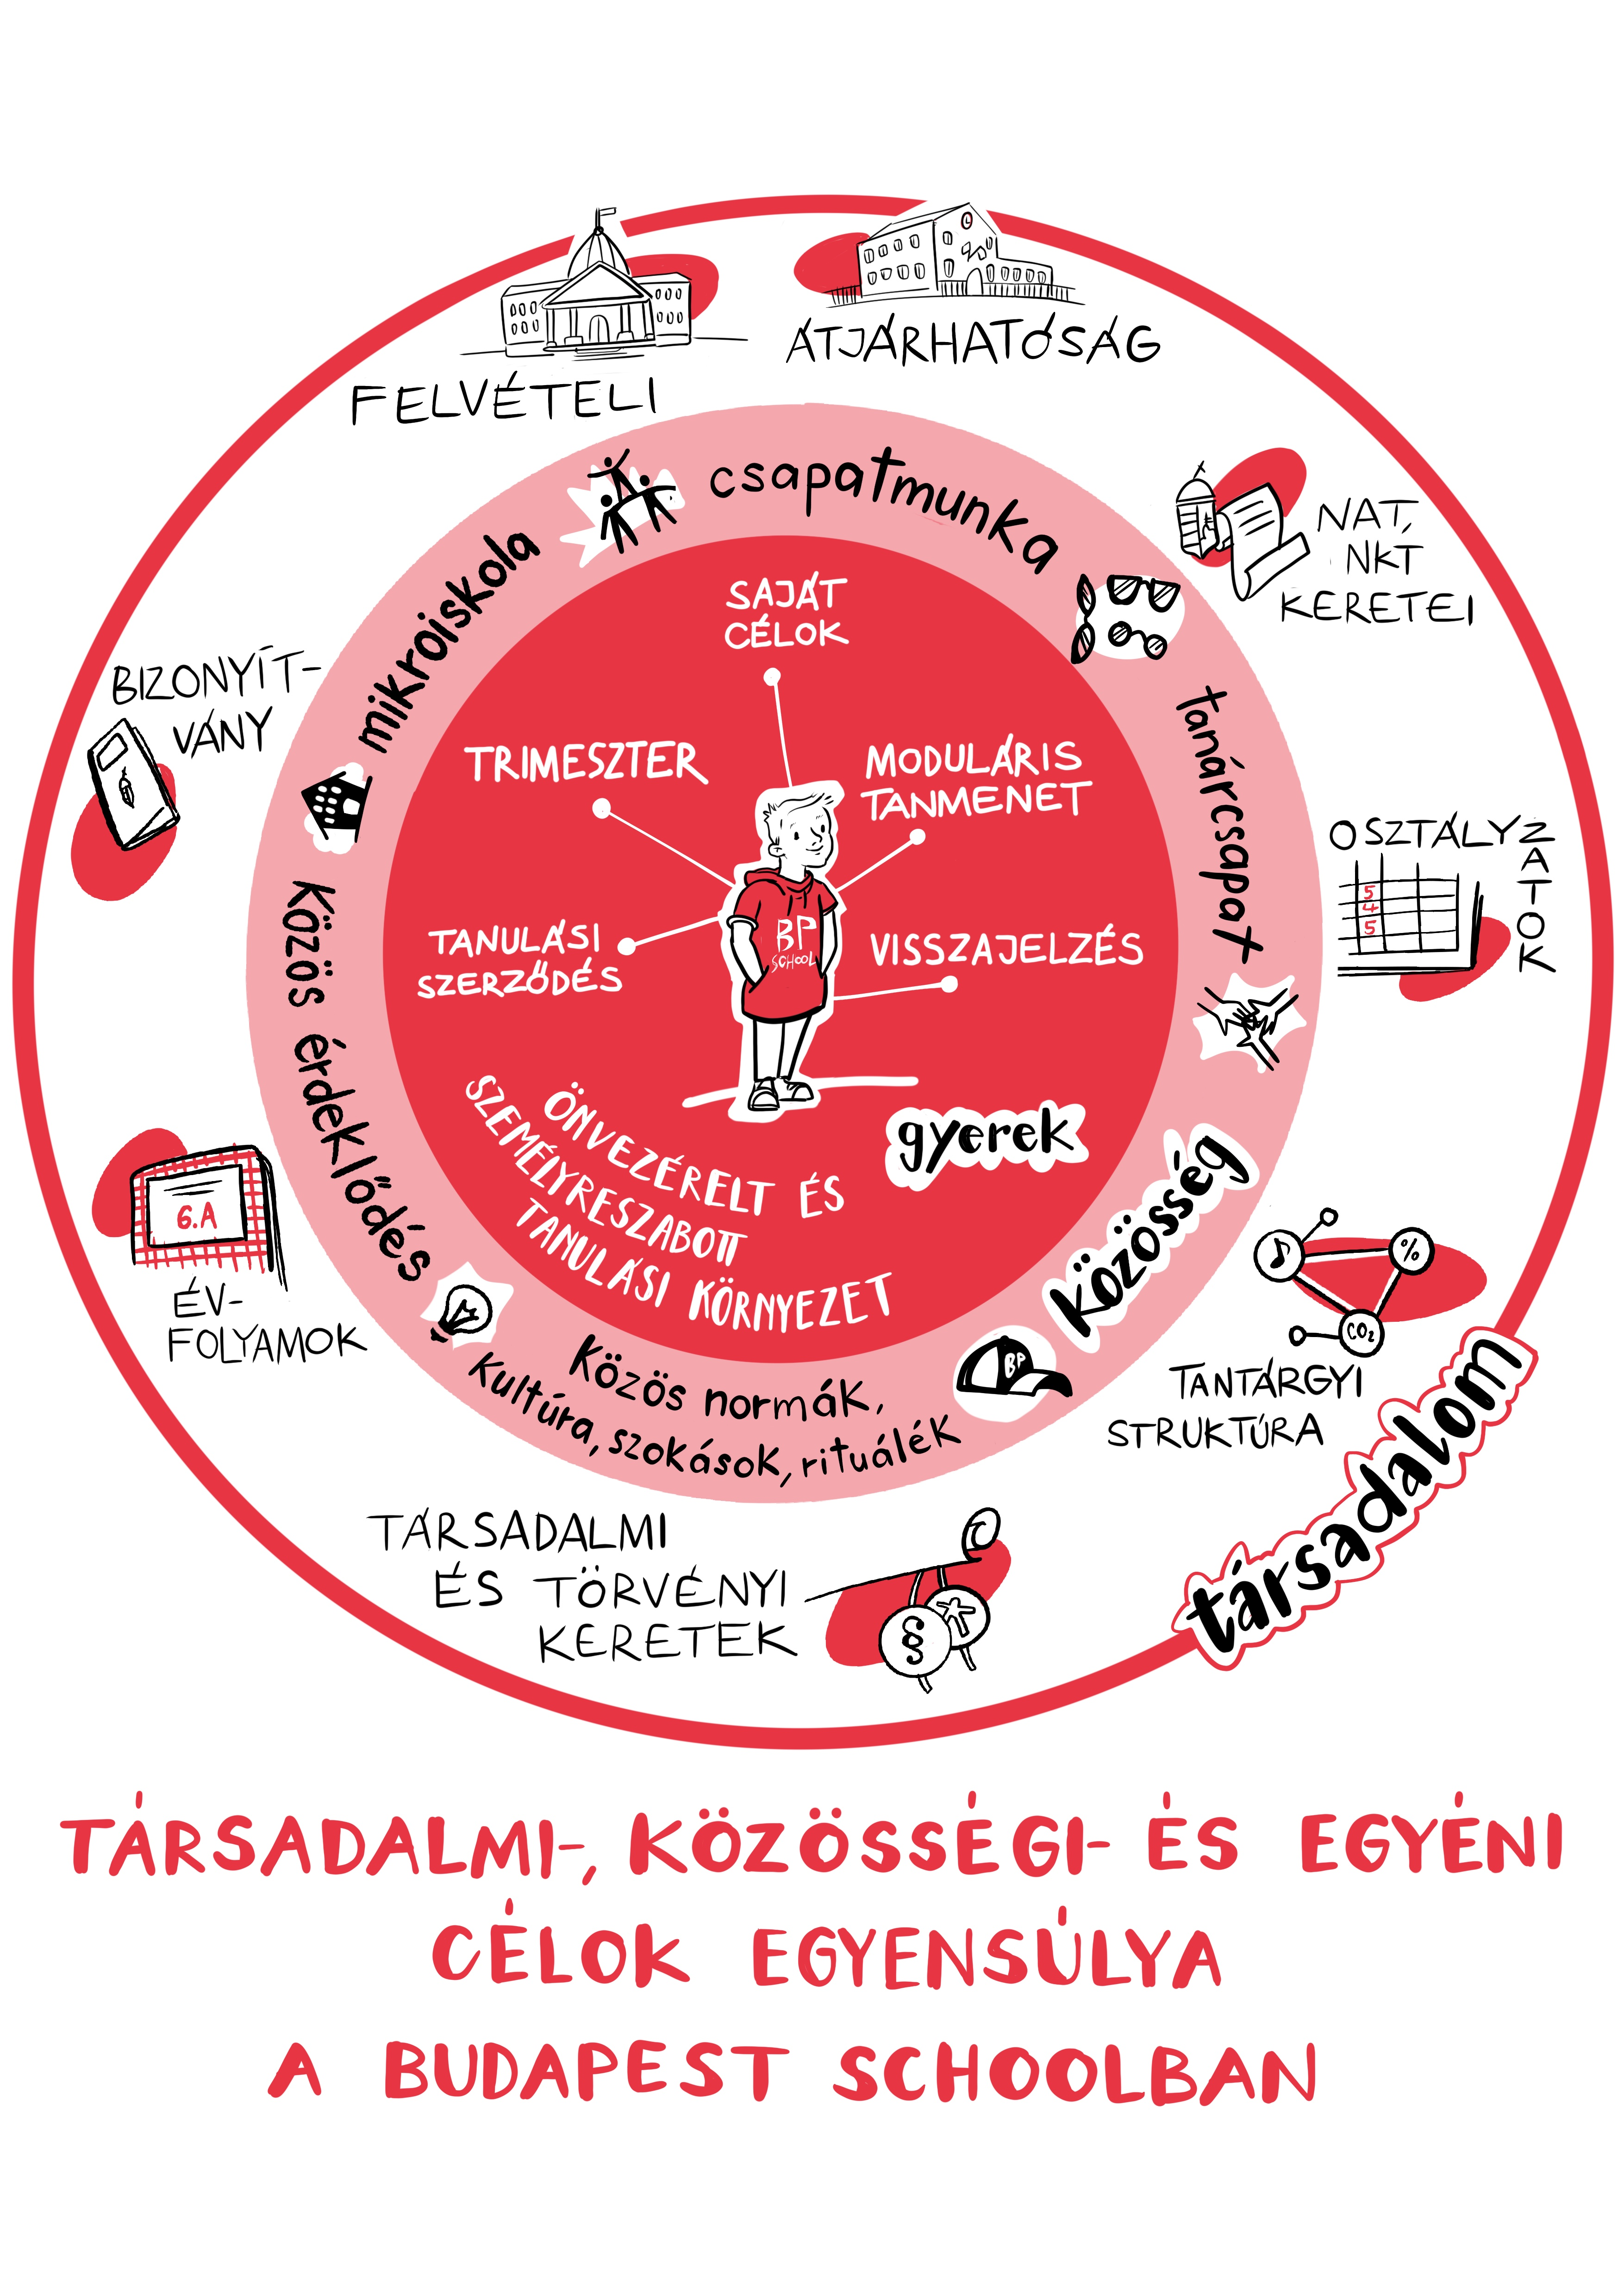
\includepdf{pics/CELOK_EGYENSULYA.JPG}

\paragraph{Egyéni és közösségi szempontok} A kerettanterv bemutatja,
hol, milyen\linebreak
módon, kitől és mit tanulhat egy Budapest Schoolba járó gyerek.
A gyerekek igényeire gyorsan reagáló mikroiskola egy buborék a gyerek körül. Ebben a körben a kerettanterv a tanulás folyamatát szabályozza, a \emph{mit tanulunk?} kérdés mellett a \emph{hogyan szervezzük meg a tanulást?} kérdésre ad választ. A tanulás során a gyerekek a kerettantervben részletezett módon az érdeklődésüknek megfelelően specifikus tanulási egységeket, vagyis modulokat végeznek el, melyek eredményeit a saját portfóliójukban gyűjtik össze. Így a gyerekek tanulási útja a portfólió fejlődésével nyomon követhető, és a portfólió tartalma alapján megállapítható a gyerek aktuális tudása, képessége. Az iskola fő funkciója emellett mindvégig az aktív tanulás, saját fejlődésük kereteinek megtalálása, a folyamatosan újragondolt saját célok állítása, és e célok irányába történő haladás marad.
 
A Budapest School kerettanterve a gyerekek, tanárok és a szülők közös döntésére bízza, hogy a gyerekek mit és hogyan tanulnak a kerettantervben meghatározott kereteken belül. A kerettanterv a specifikus célkitűzés-tervezés, a tanulás, és az arra történő reflektálás módját írja le, vagyis a tanulás folyamatát rögzíti, míg annak pontos tartalmában szabadságot enged.

\paragraph{Társadalmi szempontok}  Ezt a szabadságot keretezik a társadalmi normák és jogszabályi elvárások, hogy biztosítva legyen a mikroiskolán kívüli boldogulása is a gyerekeknek. A kerettanterv
 tantárgyi specifikációja a miniszter által kiadott kerettantervekre \citep{ofi:kerettanterv} épül, azokat strukturálja újra úgy, hogy megtartja annak tantárgyi struktúráját. A kerettanterv a tantárgyak tartalmát tanulási eredmények halmazaként adja meg. A tanulási eredmények féléves bontása, és a tantárgyi specifikációk lehetővé teszik a személyreszabott portfóliók osztályzatokra váltását egy átlátható folyamaton keresztül.

A tantárgyak lefedik a Nemzeti alaptanterv kiadásáról, bevezetéséről és alkalmazásáról szóló 110/2012. (VI. 4.) Korm. rendeletben leírt (a továbbiakban: NAT) műveltségi területeket, fejlesztési célokat és kulcskompetenciákat, 100\%-ban megfelelnek a miniszter által kiadott kerettantervek tantárgyi struktúrájának és az óraszámok is kevesebb mint 30\%-ban térnek csak el. A félévenkénti osztályzatok biztosítják az átjárhatóságot és a továbbtanuláshoz szükséges feltételeket. A kettős rendszer, a személyre szabott belső buborék és a kiszámíthatóságot adó külső kör biztosítja, hogy a 12.~évfolyam végén a gyerekeknek lehetőségük van arra, hogy érettségi vizsgát tegyenek.

\paragraph{Pedagógiai módszerek}
A kerettantervünk semleges a pedagógiai módszerekkel kapcsolatban, a tanár feladatának tekinti, hogy mindig az optimálisnak tűnő tanulási, tanítási, gyakorlási módszert válassza. Ezért ez a kerettanterv nem beszél arról, hogy a modulokat (foglalkozásokat, tanórákat) milyen pedagógiai módszer alapján szervezi a tanár.

A kerettantervünk az iskolába járókat gyerekeknek hívja, nem tanulóknak és nem diákoknak. Ennek fő oka, hogy a rendszerünkben a tanárok és a szülők is tanulók, sőt az egész iskola egy tanuló szervezet, így a kerettanterv nem akarja  kizárólag az iskola egyik szereplőjére alkalmazni ezt a szót. Másodsorban a kerettanterv hangsúlyozza, hogy a \emph{család} fontos szerepet kap a Budapest School rendszerében: az iskolában a szülők, a gyerekek és a tanárok együttműködésben dolgoznak a fejlődésért. Azok a gyerekek, akik tanulmányaik vége felé felnőtté érnek a Budapest Schoolban, tanulók is maradnak, és talán egy kicsit gyerekek is, ezért a szóhasználaton miattuk sem változtatunk. Az ő esetükben a gyerek az iskolába járó tanulót jelenti.




\section{A tanulni tanulás hét pillére}
A tanulás egyénenként változó, és ha vegyes korosztályokban is, mégis egy közösségben valósul meg. \emph{A tanulni tanulás hét pillére} minden korosztályban állandóan befolyásolja és keretezi a Budapest School pedagógiai programját.

\subsection*{Tanulni tanulunk -- fejlődésközpontúak vagyunk}
A Budapest School mikroiskoláiban mindig ott, akkor és annak kell történnie a gyerekekkel, ami őket a fejlődésükben a leginkább támogatja. Minden, ami az iskolában történik, újra és újra erre az alapkérdésre kell hogy visszatérjen. Az segíti a leginkább a gyerekek fejlődését, amit most csinálunk, vagy változtatnunk kell rajta? A Budapest School tehát rugalmas és integratív, a gyerekek fejlődéséhez igazodó.

A gyerekek tanulása \emph{fejlődésközpontú szemléletben}
\citep{growthmindset}\linebreak
(growth mindset) történik.  Erőfeszítéseik segítségével képességeik
fej-\linebreak
leszthetők, megváltoztathatóak. Számukra inspiráló a kihívás, és a hibázás kevésbé töri le lelkesedésüket. A gyerekek és a tanárok számára ezáltal nagyobb fontossággal bír a tanulásba fektetett erőfeszítés és a fejlődés, mint az aktuális képességeik.

A hibázás inkább válik a gyakorlás és az új megismerésének jelzőjévé. Ennek feszültségmentes kezelése kulcsfontosságú abban, hogy a gyerekek merjék feszegetni a saját határaikat, hogy magabiztosan dolgozzanak azon, hogy képességeiket, ismereteiket vagy gyakorlataikat folyamatosan fejlesszék. A hibázásból való tanulás fő célja, hogy mindig új hibákat ismerjenek meg, és a korábbiakra minél jobb megoldásokat találjanak a gyerekek.

\subsection{Tanulni tanulunk -- saját célokat állítanak}
A gyerekek saját erősségeiket fejlesztve saját célokat állítanak, közben céljaikat folyamatosan igazítják a világ adta lehetőségekhez és szükségletekhez.

A tanulás egésze egy olyan folyamatként írható le, amely különböző állomásokra, rövid célokra bontható. A tanulási célok állításának folyamata, annak minősége az évek alatt folyamatosan változik, egyre tudatosabbá, pontosabbá, komplexebbé válik. Azonban már az első évektől el kell kezdeni annak gyakorlását, hogy később kialakulhasson a saját tanulásicél-állítás.

A kisgyerekkor jellemzője a kíváncsiság, az igény a felfedezésre, tapasztalásra. A gyerekek számára  \emph{a tanulás  egy önvezérelt aktív folyamat}, melynek megtartása és folyamatos fejlesztése a Budapest School tanárainak legfőbb feladata. Két út van: vagy megtanítjuk a gyerekeket azokra a képességekre, amelyekre ma szükségük van, ezzel kockáztatva azt, hogy a tanulásuk a világ változásával veszít korszerűségéből, vagy abban segítjük őket, hogy megtaníthassák magukat azokra a képességekre, amelyekre épp az adott élethelyzetükben szükségük van. A tanulás így élményszerűvé válik, ismeretszerző jellege csökken, és nő az önálló felfedezés lehetősége.

\subsection{Tanulni tanulunk -- mindig és mindenhol}
A tanulás a Budapest Schoolban egész nap történik, melynek pontos alakítása a gyerekek tanulási igényeitől, fejlettségi szintjétől és korosztályától is függ. A tanulási rend meghatározásáért a Budapest School mikroiskoláinak tanulásszervezői felelnek.

A tanulás trimeszterenként újraszervezett módon tanulási modulokban történik, melynek során jut idő egyéni és csoportos, gyakorló, ismeretszerző és gyakorlatias foglalkozásokra is. Az egész napos iskola lehetőséget biztosít arra, hogy a tanulási egységek között legyen idő fellélegezni, és felkészülni az újabb modulokra, valamint arra is, hogy ha egy tanulási egység nagyon magával ragadja a gyerekeket, akkor benne maradhassanak és annak megfelelően alakítsák újra az időrendjüket.

A tanulás az iskolában nem ér véget. A tanulás szeretetének kialakulásával folyamatossá válik az ezzel való foglalkozás, így a Budapest School tanulásnak veszi az otthon, szünetekben eltöltött időt is, ahol sokszor hatékonyabb módon tud egy gyerek gyakorolni, kutatni, alkotni, mint az iskolában, amikor társaival van egy közösségben és ezáltal számos más inger is éri.

Az iskolában történő tanulással egyenrangúnak tekintjük az otthon tanulást, az iskolától független iskola utáni programokat, a (nyári) táborokat, a családi utazásokat, a vállalatoknál töltött gyakornoki időt, az egyéni tanulást és projekteket. A tanulás bárhol és bármikor történhet, és célunk, hogy mindenhol és mindig tanuljanak.

\subsection{Tanulni tanulunk -- együtt, egymástól}

A tanulás egyénileg és csoportokban is történhet. A csoportok megszervezése mindig azon múlik, hogy az adott tanulási célt mi szolgálja a legjobban. Ennek megfelelően a gyerekek nem állandó, hanem a tanulási célokhoz, az érdeklődéshez, a képességi szintekhez alkalmazkodó rugalmas csoportokban tanulnak. A tanulás ezáltal kevert korcsoportokban is történhet, akár egy nagy családban. Együtt, egymástól tanulnak a gyerekek, egymást segítik a fejlődésben. Az egymásnak adott fejlesztő visszajelzések, pozitív megerősítések révén folyamatosan alakul ki a tanulás tisztelete és a képességek fejlesztésébe vetett hit.

A közösségben tanulás módja nagyban függhet attól, hogy egy gyerek mennyire zárkózott, mennyire tud és akar önállóan tanulni. A csoportos munkák során alapelv, hogy a zárkózott gyerekek is lehetőséget kapjanak, hogy csöndesen, vagy kisebb csoportban végezhessék a munkájukat, mondhassák el ötleteiket. Az egyéni tanulásban minden gyereknek lehetőséget kell adni arra és segíteni kell abban, hogy önállóan, fókuszáltan tudjon tanulni.\vfill\eject

\subsection{Tanulni tanulunk -- alkotnak és felfedeznek}
A tanulás három rétege, az ismeretszerzés, a gondolkodás fejlesztése és a gyakorlatias, aktív alkotás egyszerre jelenik meg a Budapest School mindennapjaiban. Az alkotó munka rugalmas időkereteket, változó csoportbontásokat, és a projektmódszerek sokszínű alkalmazását igényli. A tanulás ilyenkor sokszor csinálássá válik, az ismeret pedig termékké változik.

A gyerekek önmaguk és a világ számára releváns kérdésekkel foglalkoznak, amihez külső szakértőket is bevonnak, ha szükséges. A tanulás tehát célokhoz és nem tárgyakhoz kötött. A tanulás tartalmát igazítjuk a tanulás céljához, ezáltal az egyes tudományterületek, művészetek, vagy épp mesterségek gyakran keverednek egymással egy-egy modulon belül. Szintén a célhoz igazított tanuláshoz kötődik a kutató-felfedező attitűd, ami a már ismert újramegismerése mellett az ismeretlen felfedezésére, a megválaszolhatatlan megválaszolására irányul.

\subsection{Tanulni tanulunk -- elfogadóak és egymásra figyelnek}

A gyerekek tanulását családi hátterük változása, egyéni problémák, számos mindennapi esemény befolyásolhatja. Ezek figyelembevétele a mindennapokban, a \emph{mentor tanárral} való bizalmi viszonynak köszönhetően válik lehetségessé. Ennek a kapcsolatnak az alapjait ezért a partnerség, az értő figyelem adja.

A Budapest School emellett kiemelt figyelmet fordít arra, hogy a sajátos nevelési igényű tanulók is lehetőséget kapjanak a csoportban való munkára, amennyiben az a közösség számára is hasznos. Tanulásukat, ha szükséges, külső szakember segíti. A Budapest School a hátrányos helyzetű gyerekek számára is biztosítani kívánja az elfogadó, fejlesztő környezetet. Az egyenlő bánásmód megvalósulása érdekében olyan differenciált tanulási környezetet alakít ki, ami biztosítja a minél nagyobb mértékű inkluzivitást.

\subsection{Tanulni tanulunk -- tanulva tanítunk}
A Budapest School \emph{tanulásszervezői} partnerként, a tanulás folyamán segítő társként vannak jelen a gyerekek életében. A tanulás tanórák helyett pontos tanulási célokat tartalmazó tanulási modulokból épül fel, melyek során a tanár az adott cél eléréséhez szükséges eszközöket, tanulási segédleteket biztosítja.

A tanár akkor és annyira segíti a gyerekeket a saját céljuk elérésében, amennyire azt a gyerek igényli, és folyamatosan tekintettel van arra, hogy a gyerek saját fejlődési üteme megvalósulhasson. Ehhez tudatosan kell kezelnie nemcsak a gyerekeket érintő fejlesztési lehetőségeket, hanem azt is pontosan látnia kell, hogy egy adott tanulási cél elérésének milyen készségszintű vagy gyakorlatias alapfeltételei vannak. Ezért a gyerekek tanulási célját támogatandó segítenie kell abban, hogy a gyakorló idő, a gyakorlatias alkotó idő és az új ismeret megszerzésének ideje folyamatos egyensúlyban legyen. A tanár a gyerekekkel együtt fejlődik, saját tanulása a segítői szerepben folytonos.

\label{sec:alapelvek}
\section{Emberkép}
\label{sec:gyerekkep}

A világ és benne az egyén állandóan változik, és a változás mégis számos állandóságot jelöl ki. Korábban a technológiai változás évszázadokban volt mérhető, az általunk használt eszközök száma és komplexitása jóval kevesebb volt, mára néhány év, vagy egy pár órás repülőút elegendő ahhoz, hogy olyan környezetbe, olyan emberek, eszközök közé kerüljünk, ahol másként kell alkalmazkodnunk, mint ahogy azt tanultuk. Ebben a világban a saját belső harmóniánk megtalálása, a saját közösségünkhöz, közösségeinkhez való kapcsolódás, a világ működésének megértése és a törekvés arra, hogy tegyünk a fenntartásáért, különösen fontossá vált. Ahhoz, hogy ennek megfeleljünk, a tanári, szülői és a tanulói szerepekben is folyamatos fejlődésre van szükségünk. A jövőbe nem látunk, de egy dolgot biztosan tudunk: bármilyenek is lesznek a jövő kihívásai, nekünk az a fontos, hogy ez a gyerekek számára ne félelmetes és szorongást keltő legyen, hanem lehetőséget, kihívást és örömet okozzon.

A célunk, hogy a fiatalok az iskolában és utána is könnyen megtalálják a saját útjukat. Képesek legyenek önmaguknak célokat állítani, azokat elérni. Képesek legyenek már kisgyerekkortól sajátjuknak megélni a tanulást és ahhoz kapcsolódóan célokat elérni, és fokozatosan tanulják meg azt, hogy egyénileg és csoportosan is tudjanak nagyszabású projekteket véghezvinni. A tanulás három rétege, a tudás megszerzése, az annak felhasználását segítő önálló gondolkodás és az aktív alkotás egyszerre jelenik meg a mindennapokban. Ezek egyensúlyban tartása éppoly fontos, mint az, hogy a Budapest School kerettantervének megfelelően a saját célok legalább 50\%-ban a kerettantervi tanulási eredményekből és további 50\%-ban ott nem felsorolt célokból épüljenek fel. Saját célként a sajátnak megélt célokat értjük.

Ezért \emph{legfontosabb fejlődési dimenziónak az önálló, célorientált tanulási és stratégiai gondolkodást tekintjük}, melynek ütemeit tanulási szakaszokra bontjuk. A társas kapcsolatok tanulási folyamatában a születéstől a felnőttkorig a teljes magára hagyatottság és énközpontúság csecsemőkori állapotából fejlődik az ember önállóan és kreatívan gondolkodó, önmagával és közösségével integránsan élő érett nagykorúig. Ezt az utat Erik Erikson pszichoszociális fejlődési modelljében rögzítette \citep{Erikson91}. A Budapest School ezt a modellt integrálja tanulási struktúrájába, melynek eredményeképp az iskolakezdőtől az érettségizőig négy tanulási szakaszt különít el. Ezen tanulási szakaszok határait az önállósodás során tapasztalt egyéni mérföldkövek jelölik ki, melyek fokmérője a saját cél állításának időbeli, tartalmi előrelépései, valamint az egyén belső szabadságérzete és közösséghez való kapcsolódása. Amellett, hogy az egyes tanulási szakaszok  a célállításban elkülönülnek egymástól, a szintugrás abban is mérhető, hogy mennyire képes egy gyerek az alatta lévő szinten lévő társait segíteni az előrelépésben. A folyamatos kortárs támogatás a szintekben való előrehaladás valós fokmérője a mentor és a szülő visszajelzései mellett.

\paragraph{Első szint, 5--10 év }

Ebben a korban alakul ki a gyerekek logikus gondolkodása, melynek részeként feladatokat tudnak rendszerezni, sorrendeket képesek felállítani és azokat fogalmakhoz társítani. A gondolkodásuk elkezd a befelé fordulóból a társas kapcsolatok irányába nyílni, ezáltal megnyílik a közösségi problémamegoldás lehetősége. Igényük nő a belső és a külső rendezettségre, így elkezdhetnek önmaguk szabályokat alakítani a saját tanulási igényeik kapcsán. Az első szakaszban a gyerekek pszichoszociális fejlődésükkel összhangban a saját maguknak állított cél jelentőségének fogalmát tanulják rövid, eleinte néhány órás, majd a szakasz vége felé néhány napos tervezéssel és erre adott önreflexiókkal és külső megerősítésekkel.  Megtanulják a ma, a tegnap és a holnap fogalmát. Tanulási szerződésük tartalmát eleinte főleg a mentor és a szülő segítségével állítják össze, hogy annak a szakasz végére már teljesen egyedi, önállóan kiválasztott elemei is lehessenek.

Ebben a szakaszban a szabad játéknak még nagy szerepe van, a belső világ tágassága fokozatosan nyílik meg a külvilág felé, és kezd lényegessé válni az azokkal való kommunikáció kiérlelése. Ekkor tanulnak meg a gyerekek írni, olvasni, és megismerik a matematikai alapműveleteket, valamint a mindennapjaikban használatos  geometriai és kombinatorikai alapfogalmakat, mely tudás a mindennapjaikba beépülő önálló tanulási célokhoz kapcsolódóan folyamatosan egyre szükségesebbé válik. Önmagukhoz és környezetükhöz érzékenyen, odafigyeléssel és empátiával fordulnak, megtanulják tiszteletben tartani, hogy társaik másmilyenek, akiket más dolgok is érdekelhetnek, másfajta megoldásaik is lehetnek. \emph{A szakasz végére biztonsággal meg tudnak maguknak tervezni egy néhány napos projektet.}\eject

\paragraph{Második szint, 9--14 év}

A gyerek testi és pszichoszociális fejlődése szempontjából egyaránt kiemelten fontos időszak következik. A korai serdülőkorban alakulnak ki a másodlagos nemi jellegek, melyek ütemükben mind a fiúk és lányok, mind az egyének között jelentős eltéréseket mutathatnak. Az egyéni tanulási tervek összeállításának ezért ebben az időszakban megnő a szerepe.

Az agyi struktúrák jelentős átalakulása is erre az időszakra tehető, a gondolkodás, a figyelem, az emlékezet területén is lehetnek ezen átalakulások miatt nehézségek, amit később, az átmeneti visszaesést követően az agy magasabb minőségű működése követi. Ekkor alapozhatja meg egy gyerek a tervezés, a saját tanulási célok komplexebb fogalmait. Aki ebbe a szakaszba lép, már hetekre előre ki tudja jelölni a saját feladatait. Három év alatt oda akar eljutni, hogy a szakasz végére önállóan képes legyen egy teljes trimeszternyi tanulási tervet összeállítani. Ehhez a hetek számát folyamatosan növelnie kell, miközben a problémák komplexitása is változik. A szülő még mindig megjelenik a célalkotásban, de egyre inkább átalakul a szerepe tanácsadóvá. A mentor az egyéni fejlődés mintázataira figyelve segíti a gyereket abban, hogy fejlettségi szintjének, aktuális testi, lelki változásainak megfelelő módon legyen terhelve.

\emph{A szakasz végén önállóan be tudja mutatni társainak egy pár hetes projekt eredményeit, és mind szövegértése, mind logikus gondolkodása és matematikai alapismeretei olyan szinten állnak, hogy elmélyült alkotó, kutató feladatokat vállalhat a következő szakaszban.} Biztonságos nyelvhasználata a sajátja mellett már egy másik nyelvben is elkezdődik, és értékrendjében önmaga és társai megismerésén túl a környezet és a világ fogalma is tágulni kezd.

\paragraph{Harmadik szint, 12--16 év}

A sajátként megélt tanulási célok eddigi alapozása ebben a szakaszban nyeri el mélyebb funkcióját. A tinédzserkor minden szempontból a gyerek kivirágzásának időpontja, melynek során a helyét kereső, befelé, saját változásaira fókuszáló gyerekből egy, a jövő felé nyitott kamasz válhat. A gondolkodási struktúrák mellett megnő a családon túli társas kapcsolatok szerepe, és ekkor fontos, hogy a családias jelleg, a biztonságos tanulás, a szülővel való konzultáció mint a gyerek számára egyaránt fontos érték, és nem mint kényszer jelenjen meg. Az érvelés, a hipotézis-alapú problémamegoldás, valamint a jelen fókuszált megélése ebben a korban alakul ki, ahogy annak a tudata is, hogy tetteinknek a jövőre nézve nagyobb mértékű következményei lehetnek. Kiemelten fontos ebben a szakaszban a különböző vélemények, információk, megoldási lehetőségek számba\-vétele, annak lehetősége, hogy a gyerek egyénileg ismerhesse fel az eltérő utak közötti különbségeket, és ha teheti, kérdőjelezzen meg akár tudományos hipotéziseket, vagy írjon újra művészeti, kulturális tartalmakat.
Ha a gyerek ezen határok megértésében szabadon fejlődik, akkor lehetősége lesz arra, hogy a megszerzett alapjait olyan kreatív irányokba fordíthassa, melyek saját élete és társadalmunk jövője formálásához egyaránt hasznosak lehetnek. \emph{Ebben az időszakban a saját tanulási célokat egy teljes trimeszterre vonatkozóan egyénileg határozza meg a gyerek, a szülő és a mentor ebben mint konzulens jelennek meg. Meghozza első komolyabb döntéseit arról, hogy milyen területekkel szeretne elmélyültebben foglalkozni, és ehhez kapcsolódóan választott érettségi tantárgyait is kijelöli a szakasz végére.} Előadásmódját, kutatási és alkotói munkáját felnőtt jegyek jellemzik.

\paragraph{Negyedik szint, 15--19 év} Ebben a szakaszban a gyerek fizikai
értelemben teljesen felnőtté válik. Érzelmi és szociális biztonságra azonban kiemelten szüksége van. A szerelem, a szexuális identitás erősödése, az önállósodásra való igény, az addikciók veszélye konfliktusokat szülhet, melyek kezelése különösen fontos ebben az időszakban. Az iskola elsődleges feladata ennek a biztonságos közegnek a megteremtése ebben a felnőttszerű időszakban. Ebben a mentor a szülővel együttműködve tudja segíteni a gyereket. A szakasz célja, hogy a gyerek képessé váljon a saját életét meghatározó, egy-két éves távlatokban mérhető felelős döntések meghozatalára, melyek akár sorsfordító jelentőségűek is lehetnek. Ezek a döntések  vonatkozhatnak egy emelt szintű érettségire való felkészülésre, egy nemzetközi egyetemre való felkészülésre, egy nagyobb komplexitású kutatási vagy alkotói projektre. Fontos azonban a gyerek támogatása abban is, hogy nem kell örök érvényű döntéseket hozni. Ekkorra már megtanult szakaszosan célokat állítani, és tudja, hogy bármikor lesz lehetősége az életben újratervezni. Önállóan készül az érettségire, tanárai segítik, hogy folyamatosan megtalálja a kihívást ebben. Saját céljai szűkebb környezetén túl könnyedén hatással lehetnek már a világra is.

\section{Kapcsolat a hazai és nemzetközi oktatási reformokkal}
\label{sec:kapcsolat_reformokkal}

A Budapest School programja a hazai és nemzetközi oktatási reformok kontextusában és a pszichológia, a szociálpszichológia, valamint a szervezetfejlesztés terén elvégzett kortárs kutatások tükrében válik könnyebben értelmezhetővé.

Magyarországról több iskola története, működése is nagy hatással volt ránk. A 90-es évektől induló alternatív iskolák világát mi a \emph{Rogers Személyközpontú Általános Iskola}, a \emph{Lauder Javne Iskola}, a \emph{Kincskereső Iskola} és a \emph{Gyermekek Háza} alapján ismertük meg. A megújuló középiskolák modelljének mi az \emph{Alternatív Közgazdasági Gimnáziumot} és a \emph{Közgazdasági Politechnikumot} tartjuk. Ezek az iskolák a személyközpontúság, a gyerekközpontúság hangsúlyozása mellett elkezdték a gyakorlatban alkalmazni a partnerség alapú kommunikációt, a differenciálás, a kooperatív technikák módszerét és egyes projektmódszertanokat. A \emph{Zöld Kakas} iskola programjának egyszerűsége és rendszerszintű szemlélete az egyik legnagyobb inspirációt adta számunka.

Programunk kidolgozásában nagy szerepe volt annak, hogy ezek az iskolák olyan szemléletmódbéli alapokat fektettek le, amelyek mára alapelvárásként fogalmazódnak meg a szülők oldaláról az iskolákkal szemben.

Gyakorlati tapasztalatokat a világ más részein is gyűjtöttünk. A 21. században a Budapest Schoolhoz hasonló kezdeményezések sorra indulnak a világban. Ezek egyes jegyei a Budapest School modelljével összhangban vannak:

A \emph{Wildflower School}\footnote{https://wildflowerschools.org/} mikroiskolák hálózatát működteti kisebb üzlethelyiségekben. A Budapest Schoolhoz hasonlóan célja, hogy falakat romboljon a gyerekek és a világ között: a magántanulás és az intézményes tanulás, a tanár és a tudós szerepe, valamint az iskola és környezete közötti határok elmosása az egyik fő üzenete.

Hasonlóan az otthon tanulás és az  \emph{unschooling} strukturált formáját keresi az amerikai Texasban alapított \emph{Acton Academy}\footnote{https://www.actonacademy.org/}, amely a szokratikus módszereket (azaz, hogy megbeszéljük közösen), a valós projekten keresztüli tanulást, és a gyakornokoskodáshoz hasonló munka közbeni tanulást (,,learning on the job'') teszi a megközelítésének középpontjába.

A \emph{High Tech High}\footnote{https://www.hightechhigh.org/} iskoláiban a gyerekek elsősorban projektmódszertan alapján tanulnak. A tanulási jogokban való egyenlőség mellett az egyéni célokra szabott tanulás, a világ alakulásához kapcsolódó tartalmi elemek, valamint az együttműködés-alapú tanulás is megjelenik pedagógiájukban a Budapest School által is alkalmazott jegyekből.

A \emph{School21}\footnote{https://www.school21.org.uk} brit iskola 21.~századi képességek fejlesztését tűzte ki célul. Ezért a prezentációs, előadói skillek kiemelt jelentőségűek. Az iskola egyensúlyt akar teremteni a tudásbéli (akadémiai), a szívbéli (személyiség és jóllét) és a kézzel fogható (problémamegoldó, alkotó) között. A Budapest School iskoláinak hasonló módon célja, hogy a tanulás három rétegét, a tudást, a gondolkodást és az alkotást folyamatos harmóniában tartsa.

A \emph{Khan Lab School}\footnote{https://khanlabschool.org/} a Montessori-módszert keveri az online tanulással. Kevert korosztályú csoportokban, személyre szabott módszerekkel segítik a képességfejlesztést és a projektalapú munkát. 
\newpage
\thispagestyle{empty}


\chaptercover{pics/chapter_covers/2d.JPG}
\chapter{Tanulás megközelítése}
\section{Pedagógiai és pszichológiai háttér}

Az iskolák gyakorlatias tapasztalata mellett a Budapest School számos elméletet is kiemelten fontosnak tart. 

Ezek közül is oktatási programjának központjában Carol Dweck fejlődésközpontú szemlélete \citep{growthmindset} áll. Emellett nagy hangsúlyt fektetünk az alábbi elméletek gyakorlati alkalmazására is:

Reformpedagógiai irányzatok elméletei, különös tekintettel:

\begin{itemize}

      \item
            Montessori-pedagógia (Maria Montessori),
      \item
            kritikai pedagógia (Paulo Freire)
      \item
            élménypedagógia (John Dewey)
      \item
            felfedeztető tanulás (Jerome Bruner)
      \item
            projektmódszer (William Kilpatrick)
      \item
            kooperatív tanulás (Spencer Kagan)
\end{itemize}

Pszichológia és szociálpszichológiai kutatások eredményei:

\begin{itemize}

      \item
            kognitív interakcionista tanuláselmélet (Jean Piaget)
      \item
            személyközpontú pszichológia (Carl Rogers)
      \item
            kommunikáció és konfliktuskezelés (Thomas Gordon)
      \item
            erőszakmentes kommunikáció (Marshall Rosenberg)
      \item
            pozitív pszichológia eredményei, különös tekintettel: flow-elmélet, kreativitáskutatások (Csík\-szent\-mihályi Mihály)
      \item
            érzelmi és társas intelligencia (Peter Salovey, John D. Mayer, Daniel Goleman)
      \item motivációkutatások, amiket jól összefoglal Daniel H. Pink műve \citep{pink2011drive}
      \item
            hősiesség pszichológiai alapjai (Phil Zimbardo)
      \item
            fejlődésfókuszú szemlélet (Carol Dweck)
\end{itemize}
\section{Pedagógia módszerek}
\label{sec:pedagogia_modszerek}

A Budapest School iskola tanárainak feladata, hogy mindig keressék azt a
módszert, azt a környezetet, ami az adott gyerekekkel, adott mikroiskolában a
leginkább működik. A módszer kiválaszatásakor mindig azt kell szem előtt
tartaniuk, hogy az a gyerekek egyéni céljaihoz, a közösség tanulási
lehetőségeihez a leginkább alkalmazkodjon. Nem tudjuk megmondani előre, hogy mikor milyen módszert érdemes választani, de
azt tudjuk, hogy mi alapján keressük a megfelelő technikákat. Vannak olyan módszerek, amelyek a
saját célok lehetőségeinek kitágítását és azok elérését nagyban támogatják.
Ezek alkalmazása javasolt a csoportmunkák és az egyéni gyakorlások alatt.

Azt is tudjuk,
hogy nem baj, ha nem elsőre találtuk meg a megfelelő módszert, hiszen a
próbálkozások során rengeteg új információt nyerünk, amelyek segítségével már
könnyebb megtalálni a valóban megfelelő megoldást. Az alábbiakban néhány a Budapest School számára meghatározó fontosságú módszert
emelünk ki.

\subsection{Projektmódszer}
Projektmódszert alkalmazó modulok során fő célünk, hogy a gyerekek aktívak és
kreatívak legyenek, és ezért a tevékenységek sokszínűségét helyezzük fókuszba.
Projektmódszer esetén is bátorítva van minden tanár, hogy a legváltozatosabb
módszertárral közelítse a gyerekeket, figyelve arra, hogy a tanár attitűdje, a
csoport dinamikája és az aktuális tevékenységek mit kívánnak.

\paragraph{A projektmunka folyamata}

\begin{description}
      \item[Téma, cél] Első lépés, hogy meghatározzuk a projekt témáját vagy
            célját. Ez jöhet a tanártól, a gyerekektől, vagy akár egy szülőtől
            is.
            Fontos,
            hogy a gyerekek a projekt témáját már önmagában értelmesnek,
            relevánsnak
            tartsák.

      \item [Ötletroham]  Egy-egy téma feldolgozását csoportalakítással és
            ötletrohammal kezdjük. Ennek célja, hogy a résztvevők bevonódjanak,
            illetve
            megmutassák, hogy nekik milyen elképzeléseik vannak az adott
            témáról,
            továbbá
            milyen produktummal, eredménnyel szeretnék zárni a folyamatot. A
            létrehozott
            produktumoknak csak a képzelet szabhat határt. Lehetnek videók,
            prezentációk,
            fotók, rapdalok, telefonos applikációk, rajzok, tablók, tudományos
            cikkek stb.

      \item [Kutatói kérdés] Ezek után úgynevezett kutatói kérdéseket teszünk
            fel,
            melyek meghatározzák a vizsgálat irányát. A kérdések feldolgozása a
            legváltozatosabb módon történhet. Az egyéni munkától kezdve, a
            forntális
            instruáláson vagy a kooperatív csoportmunkán keresztül egészen a
            dráma-
            és
            zenefoglalkozásokig minden hasznosítható a tanár, a csoport és a
            téma
            igényeihez mérten.
      \item [Elmélyült csoportmunka] A projekt azon szakasza, amikor a tervek,
            kutatások alapján az implementáción dolgozik a csapat.
      \item [Prezentáció] A létrehozott produktumokat bemutatására külön
            hangsúlyt
            kell fektetni. Ennek több módja is lehet: prezentációk,
            demonstrációk,
            plakátok, projektfesztiválok.
\end{description}

Az iskolai projektek célja egy fejlődésfókuszú tanár és gyerek számára mindig
kettős: egyrészt cél a téma feldolgozása, a produktum létrehozása, másrészt az
iskola fő célja, hogy a gyerekek, a csapatok mindig fejlesszék alkotó,
együttműködő, problémamegoldó képességüket. Ezért a projekt folyamatára való
reflektálás, visszajelzés ugyanolyan fontos, mint maga a cél elérése.

A munka során külön figyelmet kell fordítani arra, hogy mindent dokumentáljanak
a résztvevők. Lehetőleg online felületen.

\paragraph{Értékelés} A projekt során több értékelési pontot érdemes beépíteni.
A foglalkozások végén a résztvevők visszajeleznek a folyamatra, értékelik a
saját, a csoport és tanár munkáját. A folyamat végén az egész projektfolyamatot
értékelik, szintén kitérve a saját, a csoport és a tanár munkájára. A
produktumok, az eredmény értékelése csoport és egyéni szinten is megtörténik.

Értékelés fókuszáljon a folyamatra, és ne (csak) 
az eredményre, hogy fejlessze a fejlődésfókuszú gondolkodásmódot.\citep{growthmindset}


\subsection{Önszerveződő tanulási környezet}
A Sugata Mitra által kialakított módszertan (angolul Self Organizing Learning
Environment) lényege, hogy a tanárok arra
bátorítják a gyerekeket, hogy csoportban, az internet segítségével \emph{Nagy
Kérdéseket} válaszoljanak meg. A jó kérdés az, amire nem egyszerű a válasz, sőt
lehet, hogy nincs is rá egyfajta válasz. Cél, hogy a gyerekek maguk alakítsák
a folyamatot, formálják a kérdést, és találjanak válaszokat.

\begin{itemize}
      \item Tanár kialakítja a teret: körülbelül négy gyerekenként egy
            számítógép,
            amit körbe lehet ülni.
      \item Gyerekek maguk formálják a csoportjukat, sőt, még csoportot is
            válthatnak a munka során. Mozoghatnak, kérdezhetnek, ,,leshetnek''
            
            más
            csoportoktól.
      \item Körülbelül 30-45 perc után a csoportok prezentálják a kutatásuk
            eredményét.
\end{itemize}

\paragraph{A jó kérdések}
A Nagy Kérdésekekre nincs könnyű válasz. Ezek nyílt és nehéz kérdések, és
előfordulhat, hogy senki sem tudja még rájuk a választ. A cél, hogy mély és hosszú
beszélgetéseket generáljanak. Ezek azok a kérdések, amikre érdemes
nagyobb elméleteket állítani, amiket jobb csoportban megvitatni, amikről
érvelni lehet és kritikusan gondolkodni.

A jó kérdések több témát, területet (tantárgyat) kapcsolnak össze: \emph{,,Mi a
hangya''} kérdés például nem érint annyi különböző területet, mint a ,\emph{,Mi
történne a Földdel, ha minden hangya eltűnne''}.

\paragraph{Fegyelmezés nélkül}
A tanár feladata a folyamat során meghatározni a Nagy Kérdést, és tartani a
kereteket. A cél, hogy a gyerekek maguk szervezzék saját munkájukat, így
minimális beavatkozás javasolt a tanár részéről. Kezdetben, gyakorló csoportoknál, a tanárnak
sokszor kell emlékeztetnie magát, hogy idővel kialakul a rend. \emph{,,Bízz a
folyamatban!''
}
Amikor a tanár úgy látja, hogy nem megy a munka, akkor csak finoman emlékezteti
a csoportokat, hogy lassan jön a prezentáció ideje. Amikor valaki a
csoportjáról panaszkodik, akkor elmondhatja, hogy szabad csoportot váltani. Ha
valaki zavarja a többieket, akkor megfigyelheti, hogy a gyerekek tudnak-e már
konfliktust feloldani. Ha valaki nem vesz részt a munkában, akkor gondolkozhat
olyan kérdésen, ami az éppen demotivált gyerekeket is bevonzza.

\subsection{Megfontolt gyakorlás}
Ahogy \citep{ericsson2016peak} is kimutatja, bárki tudja valamennyi készségét,
képességét fejleszteni, ha megtervezetten, megfontoltan gyakorolja. A Budapest
School a hagyományosan készségtárgyként számon tartott ének, rajz, testnevelés
és technika témákon kívül nagyon sok mindent kezel készségként: írásbeli
érettségi vizsgát tenni magyarból, geopolitikai elemzéseket végezni,
hiperbolikus függvényekkel egyenletet megoldani épp annyira értelmezhetőek
készségként, mint a domináns csoporttagokkal való együttműködés, vagy az, hogy
egy stresszhelyzetben lenyugtassuk önmagunkat.

A készség-, és képességfejlesztés legjobb eszköze a megtervezett gyakorlás:
a fejlődés érdekében okosan gyakorlunk. A megfontolt gyakorlás jellemzője, hogy

\begin{description}
      \item[Világos és specifikus cél] Fontos, hogy tudjuk, mit gyakorlunk, mit
            akarunk elérni.  Lehetőleg a cél legyen mérhető és mindenképp
            realisztikus,
            elérhető.
      \item[Fókusz] Gyakorlás során egy dologra érdemes figyelni
      \item[Konfortzónán kivül kell lenni] Az edzőnek, tanárnak, trénernek
            néha
            érdemes a tanulót kicsit ,,nyomni''. Emlékeztetni, hogy mindig
            lehet
            kicsit
            többet elérni.
      \item[Folyamatos visszajelzés] Nagyon gyakran kap a tanuló visszajelzést,
            mindig tudja, hogy mikor és miben fejlődött.
\end{description}

\section{Kiemelt fejlesztési irányelvek}
\label{sec:kiemelt_fejlesztesi_iranyelvek}
A Budapest School interdiszciplináris tanulási modulok formájában szervezi az iskolai tanórákat. Ezen modulok tartalmi alapjai egy az egyben megfelelnek a miniszter által kiadott tantárgyi struktúrának. Minden modul a miniszter által kiadott kerettantervek egyes, vagy adott esetben több eredményének elérését tűzi ki célul. A tantárgyak tehát a tanulás tartalmi vázát jelölik ki, a tantárgyi struktúra pedig a hozzátartozó óraszámokkal a tanulási eredmények közötti egyensúlyt adja. 

A modulok eredményei a tantárgyakhoz a portfólión keresztül kapcsolódnak, a céljuk pedig, hogy a gyerekek folyamatosan fejlődjenek a világ tudományos megismerésében (STEM), a saját és mások kulturális közegéhez való kapcsolódásban (KULT), valamint a testi-lelki egyensúlyuk fenntartásában (Harmónia), vagyis a \emph{kiemelt tantárgyközi fejlesztési irányelvekben}. A modulok fejlesztési irányelvei útmutatóul szolgálnak a tanároknak arra, hogy az elérendő eredményekhez milyen elvek mentén szervezzenek modulokat. 

Olyan diszciplinák kerültek a fejlesztési irányelvekben összevonásra, melyek a tantárgyi struktúrára lebontva is értelmezhetőek, és melyek segítik a moduloknak a mai igényekhez való megfeleltetését. Egy modul egyszerre több fejlesztési irányelvnek is megfelelhet. Gépesíthetünk úgy egy modul során egy ökológiai tangazdaságot (STEM), hogy közben megismerjük a gazdálkodás történelmi és szocio-kulturális hátterét (KULT) és a szabad levegőn végzett munkával a testünket és a lelkünket egyaránt ápoljuk.   


\subsection[STEM]{Természet- és mérnöki	tudomány, technológia és matematika	(STEM)}\sectionmark{STEM}
\emph{A fejlesztési irányelv a miniszter által kiadott kerettanterv következő tantárgyainak fejlesztési területeire, elvárásaira épül, és azt egészíti ki a saját célokkal: biológia, egészségtan, fizika, kémia, matematika, informatika, földrajz, környezetismeret, természetismeret.}

A STEM ma már nem csak néhány tantárgy összevonása és  mozaikszóban való emlegetése miatt releváns. Az interdiszciplináris tudós-mérnöki szemlélet, a fejlesztő-kutató munka, az innováció az élet minden területén megjelenik, és nem csak eldugott laborok mérnökeinek a feladata új dolgokat felfedezni, kipróbálni, alkotni. Ezt az is mutatja, hogy a világ legnagyobb mértékben bővülő munkáinak több mint fele STEM-alapú, és ezek száma a következő évtizedekben a kutatások szerint nőni fog. A STEM a jövő nagy kérdéseit hivatott megválaszolni. Épp ezért a STEM a felfedezés és a megismerés iránti vágyat kell hogy ébren tartsa és tovább mélyítse a gyerekekben, miközben gyakorlatias alkotó módszerével fejleszti a csapatmunkát és a kitartást, valamint azt, hogy a megszerzett ismereteket új, korábban nem tapasztalt helyzetekben is alkalmazni tudják. Ez az a szemléletmód, ami egyaránt segítheti az egyén akadémiai tudásának fejlődését és a tanulás iránti hosszú távú elköteleződését.

\paragraph{STEM fejlesztési célok}
\begin{itemize}
  \item Problémamegoldási képesség fejlesztése
  \item  Matematikai gondolkodás fejlesztése
  \item  Logikus gondolkodás fejlesztése
  \item  A világ működésének mélyebb megértése a természettudományos szemléleten keresztül
  \item  Innovatív fejlesztésekhez szükséges technológiai (kódolás) és gyakorlati (maker) eszköztár megismerése és alkalmazása
\end{itemize}

A STEM komplex, tudományterületeken és a technológiai lehetőségeken átívelő megközelítése sokfelé ágazik, mégis vannak olyan alapszabályai, amelyek a tanulás során mindig jellemzik. Ahhoz, hogy folyamatos fejlődés legyen, fontos, hogy az aktuális képességekhez igazodó, nyitott, tényeken alapuló, kutatásalapú, diverz módszertanú, skálázható és releváns módon történjen a STEM területen a tanulás.

A STEM irányelv a fenti célok eléréséhez a következő egymást segítő komponensek alkalmazása javasolt:

\paragraph{Gyakorlatias tanulás elkötelezett és együttműködő közösségek hálózatához kapcsolódva}
A STEM tanulás során különösen fontos, hogy az adott területet jól ismerő modulvezetőn és a mentoron túl további innovatív és segítő közegek is támogassák a gyerekek fejlődését. Sokat hozzátehet a mindennapi élethez való kapcsolódás kialakításában, ha intézményi (pl múzeum, kutatóintézet) vagy technológiai, ipari és más STEM-hez kapcsolódó területen működő cégeknél dolgozó emberek mintákat mutatnak, vagy akár bekapcsolódnak a gyerekek mindennapos munkájába.

\paragraph{Hozzáférhető tanulási gyakorlatok, amelyek a játék és a kockáztatás eszközeit is felhasználják} A STEM tematikájú játékok segítik a gyerekeket
abban, hogy egymástól és együtt is tanuljanak, ezzel fejlesztik a kreativitásukat és a felfedezés iránti vágyukat. Ezek a felfedeztető játékok ráirányítják a fókuszt a csapatmunka fontosságára és arra, hogy miként lehet mai problémákra és kihívásokra válaszokat találni.

\paragraph{Multidiszciplináris tanulási élmények, amelyek a világ nagy kihívásaira keresnek válaszokat} A STEM legfőbb kihívása, hogy a mai kor olyan
kérdésfelvetéseit vizsgálja, amelyekre közösségi, nemzeti vagy globális szinten még nincsenek meg a válaszok. Ezek lehetnek a vízgazdálkodással, az agykutatással és annak a prevencióra, vagy épp a gyógyulásra gyakorolt hatásaival, a megújulóenergia-gazdálkodással, vagy épp az önvezető autók új generációjának technológiai irányaival kapcsolatosak. Ezek a kihívások egyúttal azt is megmutatják, hogy mely kérdések lehetnek a kultúránk szempontjából relevánsak.

\paragraph{Rugalmas és befogadó tanulási környezet} Nagyban hozzájárulhatnak a
STEM élményszerű tanulásához a nyitottan értelmezett tanulási környezetek. Az iskolai terek alkotótérré változtatásával, a természeti közegekben tett terepmunkák, vagy a korszerű technológiai platformok, mint például a VR (virtuális valóság – virtual reality) vagy AR (kiterjesztett virtuális valóság – augmented virtual reality) bevonásával a területek könnyebben megismerhetővé válnak, és újabb kérdések feltevésére sarkallhatják a gyerekeket, miközben az irányító tanárszerep helyett a kísérletező, segítő és facilitátor feladatok erősödnek.

\paragraph{A tanulási eredmények mérésének új eszköztára} A teljesítmény, a
kutatás, a kísérletezés és az alkotás kiemelt fókuszú a gyerekek STEM tanulási útja során. Kiemelt szerepet kapnak ezért a saját kutatásokra épülő prezentációk, megfigyelések, és az azokra adott értékes visszajelzések.

\subsection[KULT]{Kultúra, társadalom, kommunikáció és művészetek} (KULT)
\emph{A fejlesztési irányelv a miniszter által kiadott kerettanterv következő tantárgyainak fejlesztési területeire, elvárásaira épül, és azt egészíti ki a saját célokkal: magyar nyelv és irodalom, idegen nyelv, vizuális kultúra, dráma és tánc, hon- és népismeret, történelem, társadalmi és állampolgársági ismeretek, ének-zene.}

A művészetek és önmagunk kifejezése az őskortól segítik az embereket a túlélésben. A képzelet absztrakciós szintjének alkalmazása az egyik legfontosabb faji tulajdonsága az embernek. Ennek fejlesztése pedig globális világunk egyik legnagyobb kihívása. Ahhoz, hogy a társadalmi viták és szabályozások aktív alakítójává válhassunk, hogy megismerjük a globális világunk legnagyobb kihívásait, értenünk kell a múltunkat, a saját kultúránkat és a kultúrák szerepét általában, és ki kell tudnunk fejezni magunkat olykor szavakkal, máskor a művészet eszközeivel.

Még soha nem élt az emberiség ennyire behálózott világban, és még soha nem kellett ennyire tudatosan készülnünk arra, hogy gyerekeinknek többféle kultúrát, társadalmi hálózatot kell megérteniük, és abban eligazodniuk. Családok, munkahelyi és lakókörnyezeteink, sőt még a nemzeti és az azokat átívelő társadalmi környezetek is gyorsabban változnak ma, mint szüleink életében. Ezért szeretnénk, hogy gyerekeink stabil identitásukra építkezve képesek legyenek emberként emberekhez kapcsolódni, embertársaikat megérteni, velük együtt élni, dolgozni.

A tanulás egyik legfőbb funkciója, hogy képessé váljunk egy fenntartható élet kialakítására. Ehhez pedig önmagunk, környezetünk (Harmónia) és a világ működésének megismerésén (STEM) és fejlesztésén túl a szűk és tágabb értelemben vett kulturális tereinkhez is kapcsolódnunk kell (KULT). Meg kell ismernünk a lokális és a globális kihívásokat ahhoz, hogy értő, empatikus módon kapcsolódhassunk a saját és más kultúrákhoz, és a fenntartható fejlődés alakítójává válhassunk. A Budapest School KULT tantárgy fő célja ezért az olyan globális kompetenciák fejlesztése, amelyek a fenti cél elérését támogatják.

A KULT irányelv a következő fejlesztési területeket foglalja magába:
\begin{itemize}
  \item írott és beszélt anyanyelvi kommunikáció

  \item írott és beszélt idegen nyelvi kommunikáció

  \item mai lokális és globális kihívások megismerése a múlt kontextusában

  \item kulturális diverzitás és a kultúra mint az emberi viselkedést leíró eszköztár megismerése

  \item művészetek stílus- és formavilága

  \item művészetek mint önkifejezési eszköz a vizuális (hagyományos képzőművészetektől a digitális művészetekig) és előadó-művészetekben (dráma, tánc, zene)
\end{itemize}

Miközben világunkban egyre nő a technológia szerepe, folyamatosan nő az igény arra is, hogy képesek legyünk értelmezni és megfelelően használni az elénk táruló információt. Ennek alapja a megfelelő szövegértés, a nyelv mint írott és verbális kommunikációs stratégiának az egyéni és korosztályi képességekhez mért alkalmazása, valamint a művészeteken keresztül a kifejezés egyéb módjainak elsajátítása. Ahhoz, hogy képessé váljunk erre, megfelelő történelmi és kulturális kontextusba kell helyeznünk az elénk táruló információt, és nyitottnak kell lennünk arra, hogy ezeket befogadjuk, és a mai kor globális kihívásaihoz képest értelmezhessük.

A KULT komplex tanulási struktúrája adja meg az új információk elmélyülésének alapjait, és segít abban, hogy a mindennapos döntési stratégiáink részévé váljanak.

A KULT az alábbi képességeket fejleszti:
\begin{itemize}
  \item Empátia és együttérzés

  \item Egyéni és közösségi hiedelmek megismerése

  \item Kritikai gondolkodás

  \item A művészetek és az irodalom funkciójának megértése és a mindennapi életbe való beépítése

  \item Az etika és a morál alapkérdéseinek felfedezése és megkérdőjelezése

  \item Ismeretlen vagy komfortzónán túli ötletek befogadása

  \item Az emberiség kulturális örökségének és aktuális diverzitásának megismerése

  \item Többsíkú gondolkodás, multidiszciplináris szövegértés
\end{itemize}

A KULT irányelv a fenti célok eléréséhez a következő egymást segítő komponensek alkalmazását javasolja:

\paragraph{Helyi közösségekhez való kapcsolódás}

Tanulás során a lokális közösségek szerepe megnő, hiszen mind a saját kultúra és művészeti értékek megismerése, mind a nyelvhasználat tekintetében döntő szerepe van annak, hogy saját környezetünkben  tudjuk ezeket érteni és alkalmazni.

\paragraph{Kortárs kihívások}

A KULT alapját a kortárs művészeti értékek, a kortárs problémák és kihívások adják. Ezek ugyan mindig a múlt és a környezet kontextusában értelmezhetők, de elsődleges módszer a kapcsolat kialakítása a mai világ alkotásaival, szövegeivel, kulturális értékeivel.

\paragraph{Multidiszciplináris tanulási élmények, amelyek a világ nagy kihívásaira keresnek válaszokat}

A KULT abban segít a gyerekeknek, hogy jobban eligazodjanak a mai és holnapi világban, és olyan kérdéseket tegyenek fel, amelyek ma még megválaszolatlanok, és a jövőt formálhatják. Ehhez a művészetek, nyelvek és kultúrák találkozási pontjait, az átmeneteket is célszerű szemlélni.

\paragraph{Rugalmas és befogadó tanulási környezet}

A mai szövegek értelmezése, az online elérhető tartalmakban való tájékozódás képessége éppoly fontos, mint az idegen nyelveken történő kommunikáció elősegítése a világhoz történő kapcsolódással. Az aktuális globális kihívásokat a múltunkon keresztül érthetjük meg, amihez tanulási környezetünket folyamatosan a megismerés igényeihez képest kell formálnunk, és olyan eszközöket kell használnunk, amelyek az értelmezést segíthetik.

\paragraph{Alkotói szabadság és az alkotó szabad értelmezése}

Az önálló alkotói munka és az alkotások szabad értelmezése és befogadása az innováció és a kreativitás alapja. Ennek biztosításához a hagyományos keretek újraértelmezésére van szükség és arra, hogy egy alkotói folyamatban a saját cél kibontakozásának támogatása megtörténjen.

\paragraph{A tanulási eredmények mérésének új eszköztára}

A kommunikáció lehetőségei iránti elköteleződés, az önkifejezés és a környezetünkhöz való kapcsolódás különféle módjainak alkalmazása különösen fontos módszer. Az alkotói munka eredményei mérhetők a saját fejlődési ütemhez képest. Hasonlóképp az írott és szóbeli kifejezés, valamint a prezentáció egyéni és csoportos módjai is megfelelő mérési eszközök.

\subsection[Harmónia]{Harmónia (fizikai, lelki jóllét és kapcsolódás a környezethez)}
\emph{A fejlesztési irányelv a miniszter által kiadott kerettanterv következő tantárgyainak fejlesztési területeire, elvárásaira épül, és azt egészíti ki a saját célokkal: erkölcstan, testnevelés, technika, életvitel és gyakorlat, informatika.}

Testi és lelki egészségünk az alapja annak, hogy tanulhassunk, fejlődhessünk, és a saját életünk alakítóivá váljunk. Életünk fizikai, lelki, érzelmi és társas aspektusai határozzák meg a kapcsolódásunkat önmagunkhoz, társainkhoz és az őket körülvevő emberekhez, vagyis a tágabb értelemben vett társadalomhoz. Ez segít abban, hogy önálló döntéseket hozzunk, és jól tudjunk együtt tanulni, dolgozni csoportokban. Ahhoz, hogy a közösségünk részeként harmóniában élhessünk önmagunkkal, az épített és természeti környezetünkhöz is kapcsolódnunk kell.

A Budapest School tanulási koncepciójának középpontjában az egyén, mint a közösség jól funkcionáló, saját célokkal rendelkező tagja áll. Az iskolában való fejlődése során elsősorban azt tanulja, hogy miként tud specifikált saját célokat megfogalmazni, és hogyan tudja ezeket elérni. Ebben a folyamatban egy mentor segíti a munkáját az iskola kezdetétől a végéig. Ő figyel arra, hogy a gyerek fizikai és lelki biztonsága és fejlődése folyamatos legyen, és segíti azokban a helyzetekben, amikor biztonságérzete vagy stabilitása csökken.

A közösségben jól funkcionáló egyén belső harmóniájához ez a tantárgy a következő fejlesztési területeket határozza meg:
\begin{itemize}
  \item Érzelmi és társas intelligencia

  \item Önismeret és önbizalom

  \item Konfliktuskezelés

  \item Rugalmasság (reziliencia)

  \item Kritikai gondolkodás

  \item Közösségi szabályok alkotásában való részvétel és azok alkalmazása

  \item Csapatmunka gyakorlati fejlesztése

  \item Oldott játék

  \item Egészséges testi fejlődés

  \item Saját igényekhez képest megfelelő táplálkozás

  \item A természettel való kapcsolódás

  \item Épített falusi és városi környezetben való eligazodás

  \item A technológia világában felhasználói szintű eligazodás és annak harmonikus alkalmazása
\end{itemize}

A Harmónia irányelv a fenti célok eléréséhez a következő egymást segítő komponensek alkalmazását javasolja:

\paragraph{Közösségben, csapatban}

A Budapest School egy közösségi iskola, ahol a közösség tagjai egymással és egymástól tanulnak. A közösségekhez való tartozáshoz, a csapatban való gondolkodáshoz, és a családban való működéshez szükséges képességeket leginkább úgy tudjuk fejleszteni, ha azt kezdetektől megéljük. A közösség belső szabályainak megalkotása és az azokhoz való kapcsolódás a tanulás folyamatosságának alapfeltétele.

\paragraph{Életképességek (life skills)}

Szeretnénk, ha gyerekeink általában alkalmazkodóan (adaptívan) és pozitívan tudnának hozzáállni az élet kihívásaihoz, ha lelki és fizikai erősségük és rugalmasságuk (rezilienciájuk) megmaradna és fejlődne.	 A Egészségügyi Világszervezet \citep{oecd99lifeskills} a következőképpen definiálta  az életképességeket
\begin{itemize}
  \item Döntéshozás, problémamegoldás

  \item Kreatív gondolkodás

  \item Kommunikáció és interperszonális képességek

  \item Önismeret, empátia

  \item Magabiztosság (asszertivitás) és higgadtság

  \item Terhelhetőség és érzelmek kezelése, stressztűrés
\end{itemize}
\paragraph{Érzelmi intelligencia}

Sokszor kiemeljük az érzelmi intelligenciát, kihangsúlyozva, hogy gyerekeinknek többet kell foglalkozniuk az érzelmek felismerésével, kontrollálásával és kifejezésével, mint szüleinknek kellett.

\paragraph{Szabad mozgás és séta}

A különböző mozgásformák, sportok és a séta mindennapivá tétele természetes módon, a gyerekek saját igényei szerint kell hogy történjen.

\paragraph{Gyakorlatias, mindennapi képességek}

Ahhoz, hogy gyerekeink önállóan és hatékonyan tudják élni életüket, hogy a társakhoz való kapcsolódás ne függőség legyen, egy csomó praktikus mindennapi tudást el kell sajátítaniuk. A gyerekeknek folyamatosan fejleszteniük kell az élethez szükséges mindennapi tudást a levélszemét-kezeléstől, az internet és a szociális média tudatos használatán át, egészen a személyi költségvetés elkészítéséig.

\paragraph{Egészséges táplálkozás}

Az egészséges táplálkozás tanulható viselkedésforma, melynek alapja nemcsak a megfelelő élelmiszerek kiválasztása, hanem azok élettani hatásainak megismerése, és az étkezési szokások alakítása is.


\section{Jutalmazás és értékelés}
\label{jutalmazas}

Fontos alapelv, hogy minél inkább a folyamatot, cselekvést jutalmazzuk, értékeljünk. Tehát arra fókuszáljunk, hogy \emph{mit csinált} a gyerek, és ne arra, hogy \emph{milyen} a gyerek. Azokra a viselkedésmintákra adjunk megerősítő visszajelzést, amit látni szeretnénk a gyerekben később.  Lehetőleg kerüljük a statikus jellemzőkre, személyiségjegyekre vonatkozó értékelést. Így nem azt mondjuk, hogy \emph{,,mindig jó vagy matekból''}, hanem, hogy \emph{,,kitartóan és odafigyelve oldottad meg a feladatot''}. A Budapest School tanárai ezért nem szeretik, ha bármikor elhangzik, hogy \emph{,,tehetséges gyerek vagy''} vagy \emph{,,jaj, de cuki!''}.

Álljon itt néhány példa cselekvésre vontakozó visszajelzésre.

\begin{itemize}

      \item
            Fantasztikus, ma egy nagy kihívást választottál!
      \item
            Bátran vállaltad a rizikót!
      \item
            Nagyon jó! Tényleg sokat próbálgattad.
      \item
            Kitartóan csináltad, erre nagyon büszke vagyok!
      \item
            De jó, valami újat próbáltál ki ma!
      \item
            Köszönöm, hogy ma valakinek segítettél.
      \item
            Nagyon nagy öröm látni a haladásodat!
      \item
            Ne feledd, mindannyian tudunk a hibáinkból tanulni. Örüljünk annak, hogy ma valamit jobban tudunk, mint előtte.
      \item
            Wow, egy nehéz feladatot oldottál meg!
      \item
            Szép munka! Kipróbáltál egy másik módszert.
\end{itemize}

Az iskolában történő folyamatos visszajelzés a mindennapok része. Ezt írja le \aref{sec:ertekeles}. fejezet.

\section{A kiemelt figyelmet igénylő gyerekek}
\label{sec:kiemelt_figyelem}

A kiemelt figyelmet igénylő tanulók támogatásához  elsődlegesen a tanulásszervezőknek, mentoroknak és a modulvezetőknek kell differenciáltan, sokszínűen, türelemme és személyreszabottan megközelíteni a gyerekeket.

\begin{itemize}
      \item Mentoroknak ismerniük kell a gyerek sajátosságait. A szülőnek és a mentornak őszintén, egymást támogatva kell a gyerek egyéni támogatására felkészülni. Ehhez sokszor külső diagnózisra, szakember bevonására és a felnőttek közötti nehéz beszélgetésekre van szükség.
      \item Mentoroknak meg kell osztani a gyerekek sajátos igényeit a többi tanárral, a modulvezetőkkel, hogy ők is fel tudjanak készülni a gyerekek személyreszabott támogatására.
      \item A tanulásszervezés, a modulok, a foglalkozások, szóval minden, ami az iskolában történik  differenciálnak, egyéniesítettnek kell lennie, hogy az eltérő képességekkel bíró gyerekek is tudjanak együtt tanulni. Ahogy egy nagycsaládban is is figyelünk a különböző gyerekek eltérő igényeire, képességszintjeire.
      \item A szemléltetésnek, tevékenységeknek sokoldalúnak kell lennie, sokféle feladatot, speciális eszközöket kell használni. A gyerekek élménye változatos kell hogy legyen.
      \item El kell kérni a szülőktől a diagnózist, beszélni kell róla. Külső szakemberekkel konzultálni kell és a diagnózísban szereplő javaslatokat be kell építeni a mindennapok tervezésébe.
      \item Az egyéni haladási ütem biztosítására egyéni fejlesztési és tanulási tervet kell készíteni.
      \item A tanároknak együtt kell működni a gyermek/tanuló fejlesztésében résztvevő szakemberekkel.
\end{itemize}

Ez sok feladat, ami a tanárokra, a csoportra nagy terhet tud róni. Ezért a mikroiskolákban a kiemelt figyelmet igénylő gyerekek arányát körülbelül 20\% alatt kell tartani, hogy a támogatásukra legyen egyéni figyelem.

A fenti listából a legfontosabb elem: a tanár, gyerek, szülő hármas mellé be kell általában hívni külső, a gyerek igényeit jól értő szakembert támogatónak. A Budapest School iskola csak akkor tud segíteni, ha minden fél tudatosan áll hozzá a kiemelt figyelem szükségeléhez.
\chaptercover{pics/chapter_covers/3d.JPG}

\chapter{Tanulás szervezése}
\section{A tanulás rendszere és folyamata}

A Budapest School Általános Iskola és Gimnázium egy több helyszínen működő tanulási hálózat, amelynek célja, hogy otthonos környezetben, rugalmas, mégis jól szabályozott keretek között integrálja a NAT műveltségi területeit, fejlesztési céljait és kulcskompetenciáit a gyerekek saját tanulási céljaival. A különböző helyszínek, a Budapest School \emph{mikroiskolái}, legfeljebb hat évfolyamot átölelő összevont osztályokként, 6--60 fős tanulási közösségekként működnek (ld.~\ref{sec:mikroiskola}.~fejezet), ahol a gyerekek többfajta csoportbontásban tanulnak attól függően, hogy a Budapest School kerettantervében megfogalmazottaknak megfelelően milyen területeken kell, és milyen területeken akarnak fejlődni.

Az egyes mikroiskolákat \emph{tanulásszervező} tanárok (tanulásszervezők) csapata vezeti. Minden gyereknek van egy kitüntetett tanára, a \emph{mentora}, aki egyéni figyelmével a fejlődésben segíti (ld.~\ref{sec:tanarok}.~fejezet). Minden gyerek a mentortanára segítségével és a szülők aktív részvételével trimeszterenként meghatározza a \emph{saját tanulási céljait}
(ld.~\ref{sec:tanulasi_celok}).

A tanulásszervezők \emph{modulokat} hirdetnek ezen célokból és a kerettanterv tantárgyainak tartalmából. A modulok reflektálnak a mai világ alapvető kérdéseire, integrálják	a tudományterületeket és művészeti ágakat (tantárgyakat), és egyenlő lehetőséget adnak a tudásszerzésre, az önálló gondolkodásra és az alkotásra a gyerekek mindennapjaiban 
(ld.~\ref{sec:modulok}.~fejezet).

A kerettanterv három tantárgyat határoz meg, azok témaköreit, tartalmát és követelményeit \emph{tanulási eredmények} listájaként adja meg (ld.~\ref{sec:tanulasi_eredmenyek}). A gyerekek feladata az iskolában, hogy tanulási eredményeket érjenek el. Modulok elvégzésével tanulási eredményeket lehet elérni.

A modulok végeztével a gyerekek eredményei bekerülnek saját portfóliójukba (ld.~\ref{sec:portfolio}.~fejezet), melyek tartalmazhatnak önálló vagy csoportos alkotásokat, tudáspróbákat, vizsgafeladatokat, egymás felé történő visszajelzéseket, a fejlődést jól mérő dokumentációkat vagy bármit, amire a gyerek és tanárai büszkék vagy fontosnak tartanak. Erre a portfólióra épül a Budapest School visszajelző és értékelő rendszere (ld.~\ref{sec:ertekeles}). A portfólió alapján ismeri el az iskola az évfolyamok teljesítését (ld.~\ref{sec:evfolyamszintlepes}.~fejezet). Szükség esetén a portfólió alapján kaphatnak a gyerekek osztályzatokat is (ld.~\ref{sec:osztalyzatok}.~fejezet).

Az egyes tanulási modulok során elért eredmények a Budapest School három tantárgyában való fejlődést segítik úgy, hogy egyszerre jelennek meg benne a miniszter által kiadott kerettantervek tantárgyi elvárásai, a gyerekek saját céljai és a mai világra való integrált reflexió. Sajátként megélt tanulási útjuk során a gyerekek így egyaránt fejlődnek a világ tudományos megértésében, leírásában és újraírásában (STEM tantárgy), az emberiség művészeti, történeti és szociokulturális megismerésében, és az azt segítő kommunikáció\-ban (KULT tantárgy), valamint az önmagukhoz és környezetükhöz való kapcsolódásban (Harmónia tantárgy).
\paragraph{A tanulás rendszerszemléletű megközelítése}
Az oktatás tartalmának előzetes szabályozása helyett a Budapest School a tanulás módjára helyezi a hangsúlyt. Az iskola alapelve, hogy integratív módon folyamatosan keresse és fejlessze a pedagógiai, pszichológiai és szervezetfejlesztési módszereket, amelyek korszerű módon tudják segíteni a tanulás tanulását, az egyéni és csoportos fejlődést, a konfliktusok feloldását.

A tanulás tartalmát tekintve a Budapest School saját alternatív kerettantervére támaszkodik, amely a tanulás rendszerét, annak folyamatát szabályozza. E dokumentum alapján az állami kerettanterv tanulási eredményein történő végighaladás mellett a Budapest School nagy hangsúlyt fektet a gyerekek saját tanulási céljaira és a célállítás módjára.


\ketoldaltkep{pics/0A_SOMA.JPG}{pics/0B_FLORA.JPG}
\section{A mikroiskolák, a Budapest School összevont osztályai}
\label{sec:mikroiskola}

A Budapest School iskolában összevont osztályokban, azaz kevert korosztályú és
maximum 6 évfolyamszintű közösségben tanulnak a gyerekek. Az összevont
osztályokat a Budapest School kerettanterv \emph{mikroiskolának} hívja, ezzel
is
hangsúlyossá téve ezek egyedi jellemzőit:
\begin{itemize}
      \item A mikroiskolákban  tanulásszervező  \emph{tanárcsapatok} vezetik a
            közösségeket. 
      \item A mikroiskolák saját szabályaik, normarendszerük, szokásaik,
            kultúrájuk alakul ki.
      \item A mikroiskolák maguk alakítják saját órarendjüket, modulkínálatukat
            és ebben nem kell más mikroiskolákhoz igazodniuk.
\end{itemize}


\paragraph{A mikroiskolákat tanulásszervezők vezetik.}

A tanulóközösség fontos célja, hogy biztonságot, támogatást nyújtson, és
\emph{így} segítse a közösség tagjainak a minőségi tanulását.

A mikroiskolát az igazgató által kinevezett tanulásszervezők irányítják.
Ők felelnek a tanulás tartalmáért, a modulok meghirdetéséért és a
tanulási eredmények nyomonkövetéséért. Ők döntenek a jelentkező gyerekek
kiválasztásáról és a mikroiskola mint közösség összetételéről.

A különböző tanárszerepeket, a tanulásszervezők, mentorok és modulvezetők kapcsolódását \aref{sec:tanarok}. fejezet mutatja be.

\paragraph{Mikroiskola egy nagy csoport.}

Egy mikroiskola minimális létszáma 6 maximális létszáma 60 fő. Minden
mikroiskolának megfelelő számú olyan tanulásszervezővel kell
rendelkeznie, aki mentortanárként is végzi munkáját.

\paragraph{A mikroiskolák korkülönbségei állandók, a gyerekek együtt nőnek.}
Egy mikroiskolában fő szabály szerint legfeljebb 6 (egymást követő)
évfolyamszintnek megfelelő korosztály tanul együtt. A mikroiskola
korosztályait, és az induláskor meglévő évfolyamokszinteket a jelentkező ill. a
felvett gyerekek életkora alapján határozza meg az alapító.

A mikroiskolák korhatára, mint az összevont osztályok korhatárai, a gyerekekkel
változnak. Ettől eltérően a korhatárokat tágítani és szűkíteni évente egyszer
lehet, és
erről az iskola értesíti a szülőket minden tanévkezdést megelőző február 15-ig.
(pl. Amennyiben ezzel nem sérül a maximum 6 évfolyam elve, a korhatárok
tágíthatóak, vagy ha a legalsó vagy legfelső korosztályba tartozó gyerekek
elmentek, a mikroiskola dönthet a korhatárok szűkítéséről.)
A Budapest School mikroiskolái a 12. évfolyamig tartanak, kivéve ha a
mikroiskola valamilyen okból megszűnik.

\paragraph{A mikroiskola állandó, a gyerekek és tanárok jöhetnek és mehetnek.}
A Budapest School mikroiskolái úgy működnek, mint egy összevont osztály. A
tanulásszervező tanárok vagy gyerekek kilépése a mikroiskola fennállását nem
érinti, helyettük a mikroiskola új tanulásszervező tanárt és
gyereket vehet fel.  A mikroiskola létrehozásakor arra kell törekedni, hogy
olyan
gyerekek tanuljanak együtt, akik támogatni tudják egymást a tanulásban. A
gyerekek a mikroiskola tagjai addig, amíg ott jól tudnak tanulni, és a közösség
és a gyerek kapcsolat gyümölcsöző.

\paragraph{A mikroiskoláknak saját fókuszuk, helyszínük, stílusuk alakulhat
      ki.}
A mikroiskolák nemcsak abban térnek el egymástól, hogy kevert korcsoportban,
más korosztályú gyerekek, más érdeklődések mentén, és ily módon más célokat
követve tanulnak, hanem területileg, regionálisan is eltérőek lehetnek.

A mikroiskola-rendszerben lehetőség van arra, hogy adott tanulási környezetben
úgy váltakozhassanak a hangsúlyok a csoport és az egyén érdeklődését követve,
hogy közben
fennmaradjon a tanulási egyensúly a tantárgyak között.

Van olyan mikroiskola, amely a fejlesztési célok eléréséhez és az egyéni célok
mentén már 6 éves gyerekek tanulásánál a robotika eszközeit használja, másutt
drámafoglalkozásokkal fejlesztik 12 éves gyerekek a szövegértésüket és
éntudatukat.

\paragraph{A mikroiskolákban a tanulók nagymértékben befolyásolják, hogy mit és
      hogyan
      tanulnak és alkotnak.}
A mikroiskolákban (a tanulásszervezők által meghatározott kereteken belül)
megfér egymással több, különböző egyéni céllal rendelkező gyerek addig amíg a
tanulásszervezők minden gyerek számára biztosítani tudják a kerettantervben
megfogalmazott tanulási eredmények eléréset.

A tanulásszervezők feladata és felelőssége, hogy olyan közösségeket
válogassannak össze és építsenek, amelyek kellően diverzek, és mégis jól
működnek. A közösségnek a gyerekek igényeit és a kerettanterv céljait egyaránt
ki kell elégíteni.

A tanulásszervezők választási lehetőségeket kínálnak, (azaz modulokat dolgoznak
ki), amikből a gyerekek (a mentoruk és szüleik segítségével) a saját céljaikat,
érdeklődésüket leginkább támogató egyéni tanulási tervet és utat alkotnak.

Eltérhet, hogy egy-egy gyerek mit tanul, ezért az is, hogy mikor és hogyan
sajátítja el a szükséges ismereteket: egy közösségben megfér a központi
felvételire fókuszáló 11 éves gyerek, és az is, aki ekkor inkább a Minecraft
programozásában akar elmélyedni, ezért más képességek fejlesztésével lassabban
halad.

\paragraph{Kisebb csoportokban tanulhatnak a gyerekek.}
\label{sec:csoportbontasok}

A mikroiskolákban a közösséget kisebb csoportokra bonthatjuk, ha a
tanulásszervezés ezáltal hatékonyabb. Egyes moduloknál a gyerekek egy-egy
projektre szerveződnek, ilyenkor általában az eltérő képességű és életkorú
gyerekek is kitűnően tudnak együtt dolgozni. Más modulok esetén a csoportokat a
tanár képességszint alapján hozza létre. Ilyen csoportok lehetnek a másodfokú
egyenletek megoldóképletét megismerő csoport, az írni tanulók csoportja, vagy
egy angol nyelvű újság szerkesztésére és megírására alakult modul, ahol a
nyelvismeretnek és a szövegalkotási képességnek már egy olyan szintjén kell
állni, hogy a projektnek jól mérhető kimenete lehessen.

\paragraph{A mikroiskolák diverz, integratív közösségek.}
A Budapest School mikroiskolák társadalmi, kulturális és gazdasági értelemben
is diverzek és egyik fő céljuknak tekintik az integrációt addig, mindaddig amíg
az a közösség céljait szolgálja.

\paragraph{A mikroiskolák tanuló közösségek.}
A Budapest School célja, hogy a mikroiskolákban történő tanulás mind a gyerek,
mind a tanár, mind a szülő számára jól átlátható, követhető legyen, és gyerek
és a közösség folyamatosan fejlődjön.
A Budapest School kiemelt elve, hogy ,mindig, minden módszer, folyamat
fejleszthető, ezért a tanárok feladata, lehetősége, hogy az aktuális helyzethez
illő legmegfelelőbb módszert válasszák meg a gyerekek tanulásának segítéséhez.

\paragraph{Mikroiskolát a fenntartó indít és addig él, amíg szolgálja a
      gyerekek tanulását.}
A mikroiskolát a fenntartó indítja. Meghatározza, hogy milyen telephelyen,
tagintézményben, milyen korhatárokkal és létszámokkal
induljon a mikroiskola,. A fenntartó feladata a szükséges épületet, eszközöket
biztosítania. A
mikroiskola alapításához legalább 6 gyerek és egy tanulásszervező (aki
értelemszerűen mentortanár)
szükséges.

A mikroiskola a tanárokon és a gyerekeken is túlmutató közösség, amely akkor is
tovább működik, ha egy tanár vagy gyerek távozik. Tanulásszervező illetve
gyerek távozása esetén a mikroiskola  új tanulásszervező tanárt és gyereket
vesz fel, mindaddig, amíg a mikroiskola számára meghatározott maximális
létszámot el nem érik.

A mikroiskola abban az esetekben megszűnik meg, ha összeolvad egy másik
mikroiskolával vagy
ha a mikroiskola létszáma 6 gyerek és egy mentortanár alá csökken.

\paragraph{Gyerek csatlakozása a mikroiskolához.}
Arról, hogy egy gyerek csatlakozhat-e egy mikroiskolá közösségéhez, a
tanulásszervező
tanárok döntenek, figyelembe véve a gyerek életkorát, a közösségben való
eligazodását, érdeklődését, egyéni fejlődési igényét. Elv egyszerű: minden
gyereket fogadjon be a közösség, amitől a közösség jobban tudja támogatni az
egyének tanulási céljait.\footnote{A mikroiskolához gyerek akkor csatlakozhat,
      ha ő már másik mikroiskola, így az iskola tanulója, vagy az iskola
      igazgatója a
      gyerek felvétele mellett döntött.}

\footnote{Átjárás mikroiskolák között.}
Egy gyerek akkor válthat a Budapest School egyes mikroiskolái között,
amennyiben a fogadó mikroiskola őt elfogadja. Ilyenkor új mentortanárt kell
számára kijelölni.

\ketoldaltkep{pics/1A_MIKROISK_SOMA.JPG}{pics/1B_MIKROISK_FLORA.JPG}
\section{A tanév ritmusa}
\label{sec:tanev_ritmusa}
A tanév három trimeszter ismétlődésével írható le: a tanulási célok tervezése után következik a tanulás, és a ciklust a visszajelzés és értékelés zárja.	Amint egy ciklus véget ér, elkezdődik egy új.


Az egyes trimeszterek átlagosan 12 hétig tartanak úgy, hogy a tanítással eltöltött napok  és a tanítási szünetek mindig az EMMI által kiadott tanév rendjéhez igazodva kerülnek meghatározásra. A trimeszterek első hete mindig a tervezéssel, utolsó hete mindig az értékeléssel telik. Trimeszterenként átlagosan további egy hét a közösség építésével, önálló tanulással  zajlik.

A ciklusok állandósága adja a tanulás irányításához szükséges kereteket. Ezek megtartásáért az egyes mikroiskolák tanulásszervezői felelnek, melynek működését a fenntartó monitorozza. A tanév ritmusát \aref{tbl:tanevritmus}. táblázat mutatja.


\begin{table}
  \centering
  \begin{tabular}{ l|l }
    \textbf{időszak} & \textbf{tevékenység}                \\
    \hline
    Szeptember       &
    közösségépítés                                         \\
                     & saját célok meghatározása           \\
                     & modulok kialakítása és meghirdetése
    \\ \hline

    Október          &
    tanulás, alkotás
    \\ \hline

    November         &
    tanulás, alkotás
    \\ \hline

    December         &
    portfólió frissítése                                   \\
                     & reflexiók                           \\
                     & visszajelzések                      \\
                     & célok felülvizsgálata               \\
                     & modulok változtatása igény esetén
    \\ \hline

    Január           &
    tanulás, alkotás                                       \\
    féléves értékelés kiadása
    \\ \hline

    Február          &
    tanulás, alkotás
    \\ \hline

    Március          &
    portfólió frissítése                                   \\
                     & reflexiók                           \\
                     & visszajelzések                      \\
                     & célok felülvizsgálata               \\
                     & modulok változtatása igény esetén
    \\ \hline

    Április          &
    tanulás, alkotás
    \\ \hline

    Május            &
    tanulás, alkotás
    \\ \hline

    Fél június       &
    évzárás, értékelés, bizonyítványok
  \end{tabular}
  \caption{Egy tanévben háromszor ismételjük a célállítás, tanulás, reflektálás ciklust.}
  \label{tbl:tanevritmus}
\end{table}

A tanév három periódusból áll: ez a felosztás követi az üzleti világ negyedéves tervezését, néhány egyetem trimeszterekre bontását, de leginkább az évszakokat. Minden periódus után értékeljük az elmúlt három hónapot, ünnepeljük az eredményeket, és megtervezzük a következő időszakot.  A trimesztereken belül az egyes mikroiskolák között lehetnek néhány hetes eltérések, melyek a közösség sajátosságait követik.

\paragraph{Féléves és évvégi elszámolás}
\label{sec:feleves_bontas}
A külső rendszerekkel és a törvényeknek való megfelelés miatt a kerettanterv két félévre bontva jeleníti meg a tananyag tartalmakat, és ezzel összhangban az iskola félévenkénti értékelést állít ki automatikusan a portfólió alapján, ami nem más, mint a portfólióba bekerült értékelések összegyűjtése.

A félév vége január vége\footnote{A félév végét miniszteri rendelet évente szabályozza.}, ami a második trimeszterbe esik, ezért a féléves értékelést az első trimeszter végén rögzített állapot szerint adja ki az iskola.  Az 5--12. évfolyamszinteken lévő gyereknek januárban módjuk és lehetőségük van a portfóliójuk frissítésére, ha a féléves értékelés és az osztályzatokra váltás eredménye számukra iskolaváltás, továbbtanulás vagy egyéb okból fontos. Ilyenkor januárban alkalmuk van felkészülni \aref{sec:evfolyamok_osztalyzatok}.~fejezetben részletezett osztályzatokra váltás folyamatra.

Év végén, június hónap fele marad az évvégi zárások és igény szerint az osztályzatokra váltásra való felkészülésre, ami a portfólió frissítését, bővítését, kiegészítését jelenti.
\section{Saját tanulási célok}
\label{sec:tanulasi_celok}

Minden gyerek megfogalmazza és háromhavonta újrafogalmazza a \emph{saját tanulási céljait}: eredményeket, amelyeket el akar érni, képességeket, amelyeket fejleszteni akar, szokásokat, amelyeket ki akar alakítani. A saját célok elfogadásakor a gyerek és a mentora a szülőkkel együtt \emph{tanulási szerződést} köt.

Csak olyan célok kerülhetnek a saját célok közé, amelyek minden érintettnek biztonságosak, és amelyek összhangban vannak a tantárgyi fejlesztési célokkal és tanulási eredményekkel. A szerződésben rögzíthetőek tanulási eredményekre vonatkozó megállapodások, tantárgyi évfolyamszintekre vonatkozó elvárások (pl. ,,\emph{haladjon egy évfolyamszintet egy év alatt}'' vagy ,,\emph{készüljön fel emelt szintű érettségire}''), és a tantárgyi rendszeren kívüli célok és feladatok.

%Fontos megkötés, hogy a saját tanulási célok legalább a felének \ifkerettanterv
%      \aref{sec:tantargyi_tanulasi_eredmenyek}. fejezetben
%\else
%      a kerettanterv Tantárgyi tanulási eredmények fejezetében
%\fi felsorolt tanulási eredmények elérésére kell vonatkoznia. A másik fele szabadon alakítható.

Háromhavonta a tanulásszervezők és a gyerekek megállnak, reflektálnak az elmúlt időszakra, és a tapasztalatok, valamint az elért célok ismeretében és az új célok figyelembevételével újratervezik, újraszervezik a foglalkozások rendjét, tehát azt, hogy mikor és mit csinálnak majd a gyerekek az iskolában. A mindennapi tevékenység során tapasztalt élmények, alkotások, elvégzett feladatok, kitöltött vizsgák, tehát mindaz, ami a gyerekekkel történik, bekerül a portfóliójukba. Még az is, amit nem terveztek meg előre.

A gyerekeket a mentoruk segíti a saját célok kitűzésében, a különböző választásoknál, a portfólióépítésben, a reflektálásban. A tanulási célok kitűzése az önirányított tanulás fokozatos fejlődésével és az életkor előrehaladtával folyamatosan egyre önállóbb tevékenységgé válik. Tanulási útján, céljai kitűzésében a mentor kíséri végig a gyerekeket.

A Budapest School személyre szabott tanulásszervezésének jellegzetessége, hogy a gyerekek a saját céljuk irányába haladnak, az adott célhoz az adott kontextusban leghatékonyabb úton. Tehát mindenki rendelkezik saját célokkal, még akkor is, ha egy közösség tagjainak céljai a tantárgyi tanulási eredmények azonossága, vagy a hasonló érdeklődés miatt akár  80\% átfedést mutatnak.

A NAT műveltségi területeiben és a tantárgyakban megfogalmazott követelmények teljesítése is célja a tanulásnak, a tanulás fő irányítója azonban más. Mi azt kérdezzük a gyerekektől, hogy \emph{ezen felül} mi az ő személyes céljuk.
\section{A tanulási szerződés}

A tanulási szerződés az előbbiekben említett gyerek-mentor-szülő közötti megállapodás, ami rögzíti
\begin{enumerate}
      \item a gyerek, a mentor (iskola) és a szülő igényeit, elvárásait;\hfill\break
 ezek lehetnek: \emph{,,szeretném, ha a gyerekem naponta olvasna''} típusú folyamatra vonatkozó kérések, vagy erősebb \emph{,,változtatnod       kell a viselkedéseden, ha a közösségben akarsz maradni''} igények, határok megfogalmazása;

      \item a gyerek céljait a következő trimeszterre, vagy a tanév végéig;

      \item a gyerek, mentorok (iskola) és szülő vállalásait, amivel támogatják a cél elérését és a felek igényének teljesülését.

\end{enumerate}

A tanulási szerződésre jellemző:
\begin{itemize}
      \item A kitűzött célokat minél specifikusabban és mérhetőbben kell megfogalmazni. Javasolt az OKR  (Objectives and Key Results, azaz	Cél és Kulcs Eredmények) \citep{okr} vagy a SMART (Specific, Measurable, Achievable, Relevant, Time-bound, azaz Specifikus,  Mérhető, Elérhető, Releváns és Időhöz kötött) \citep{wiki:smart} technika alkalmazása, hogy minél specifikusabb, teljesíthetőbb, tervezhetőbb és könnyen mérhető célokat tűzzenek ki.

      \item A kitűzött célokban való megállapodást követően, megállapodást kell kötni arról is, hogy ki és mit tesz azért, hogy a gyerek a célokat elérje.

      \item A mentor a teljes mikroiskolát (a többi tanárt, a közösséget) képviseli a megállapodás során.
\end{itemize}

A tanulási szerződést néha hívjuk \emph{megállapodásnak} is. A megállapodás és szerződés szavakat ez a kerettanterv szinonimának tekinti. A \emph{learn\-ing con\-tract} az önirányított tanulást hangsúlyozó felnőttképzéssel foglalkozó irodalomban bevett szakkifejezés már a 80-as évektől \citep{Malcolm77}. Ennek a magyar nyelvben inkább a szerződés felel meg. Egy másik szakterületen, a pszichoterápiás munkában a terápiás szerződések megkötésekor a közös munka kereteinek kialakítását és fenntarthatóságát hangsúlyozzák \citep{pszichoterapia}. Erre is utalunk a tanulási szerződés elnevezéssel. Van, amikor a \emph{hármas szerződés} kifejezést használjuk, hangsúlyozva, hogy mind a három szereplőnek elfogadhatónak kell tartania a szerződés tartalmát.

\section{Különböző tanári szerepek}
\label{sec:tanarok}

A Budapest Schoolban a gyerekek azokat a felnőtteket tekintik tanáruknak, akik
minőségi időt töltenek velük, és segítik, támogatják vagy vezetik őket a
tanulásukban. Több szerepre bontjuk a tanár fogalmát: a gyerek egy (és csak
egy) felnőtthöz különösen kapcsolódik, a \emph{mentortanárához}, aki rá
különösen figyel. Ezenkívül a gyerek tudja, hogy a mikroiskola mindennapjait
egy tanárcsapat, a \emph{tanulásszervezők} határozzák meg, ők vezetik az
iskolát.  A foglalkozásokon megjelenhetnek további tanárok, a \emph{modulvezetők},
akik egy adott foglalkozást, szakkört, órát tartanak.

Szervezetileg minden mikroiskolának van egy állandó \emph{tanárcsapata}, a
tanulásszervezők. A tanulásszervezők legalább egy tanévre elköteleződnek, szemben a
modulvezetőkkel, akik lehet, hogy csak egy pár hetes projekt keretében vesznek részt a
munkában.
A tanulásszervezők általában mentorok is, de nem minden esetben. Nem lehet
mentor az, aki a gyerek mikroiskolájában nem tanulásszervező, mert nem lenne
rálátása a mikroiskola történéseire. Egy tanulásszervező lehet több
mikroiskolában is ebben a szerepben, és így mentor is lehet több mikroiskolában.

\paragraph{Mentor}
Minden gyereknek van egy \emph{mentora}, aki a saját céljainak
megfogalmazásában és
a fejlődése követésében segíti. Minden mentorhoz több gyerek tartozik, de nem
több, mint 12. A mentor együtt dolgozik a mikroiskola többi tanulásszervezőjével, a
szülőkkel és az általa mentorált gyerekekkel. A mentor segít az általa
mentorált gyereknek, hogy a tantárgyi fejlesztési célok és
a
saját magának megfogalmazott saját célok között megtalálja  az egyensúlyt, és segít megalkotni a
gyerek \emph{saját
  tanulási tervét}.

A mentor a kapocs a Budapest School, a szülő és a gyerek között.

\begin{itemize}
  \item Képviseli a Budapest Schoolt, a mikroiskola közösségét.
        \begin{itemize}
          \item Ismeri a Budapest Schoolt, a lehetőségeket, a tanulásszervezés
                folyamatait.
          \item Együtt tanul más Budapest School-mentorokkal, együtt dolgozik a
                tanártársaival.
        \end{itemize}

  \item Ismeri, segíti, képviseli a gyereket.
        \begin{itemize}
          \item  Tudja, hol és merre tart a mentoráltja, ismeri a képességeit,
                körülményeit, szándékait, vágyait.
          \item    Segít a saját célok elérésében, felügyeli a haladást.
          \item    Megerősíti a mentoráltjai pszichológiai biztonságérzetét.
          \item   Visszajelzéseket ad a mentoráltjainak.
          \item    Segít abban, hogy az elért célok a portfólióba kerüljenek.
          \item    Összeveti a portfólió tartalmát a tantárgyak fejlesztési
                céljaival.
        \end{itemize}

  \item Együtt dolgozik, gondolkozik a szülőkkel, képviseli igényüket a
        közösség felé.
        \begin{itemize}
          \item Erős partneri kapcsolatot épít ki a szülőkkel, információt oszt meg
                velük.
          \item Segít a gyerekekkel közös célokat állítani.
          \item A szülő számára a mentor az elsődleges kapcsolattartó a különféle
                iskolai ügyekkel kapcsolatban.
        \end{itemize}

\end{itemize}

A mentor egyszerre felelős a mentorált gyerek előrehaladásának segítéséért,
és
közös felelőssége van a mentortársakkal, hogy az iskolában a lehető legtöbbet
tanuljanak a gyerekek. A mentor folyamatosan figyelemmel követi az egyéni
tanulási tervben megfogalmazottakat, és ezzel kapcsolatos visszajelzést ad a
mentoráltnak és a szülőnek.

\paragraph{Tanulásszervező}
Csoportban dolgozó, iskolaszervező, strukturáló tanár. Egy mikroiskola
állandó tanári
csapatát 2--7 tanulásszervező alkotja, akik egyedileg meghatározott szerepek
mentén a mikroiskola mindennapjainak működtetéséért felelnek. Minden mentor
tanulásszervező is. A tanulásszervezők tarthatnak
modulokat, sőt kívánatos is, hogy dolgozzanak a gyerekekkel, ne csak
szervezzék az életüket.
Ők rendelik meg a külső modulvezetőktől a munkát, ilyen értelemben a
tanulási utak projektmenedzserei.

\paragraph{Modulvezetők}

Bárki lehet modulvezető, aki képes akár egy egyetlen alkalommal történő, vagy
éppen
egy egész trimeszteren át tartó tanulási, alkotási folyamatot vezetni. Ők
általában
az adott tudományos, művészeti, nyelvi vagy bármilyen más terület szakértői.

A modulokat a tanulásszervezők is vezethetik, de külsős, egyedi megbízással
dolgozó szakemberek is megjelennek modulvezetőként. Modulvezető lehet bárki,
akiről az őt megbízó tanárcsapat tudja, hogy képes gyerekek folyamatos
fejlődését és egy tanulási cél felé való haladását segíteni. A moduláris
tanmenettel \aref{sec:modulok}. fejezet foglalkozik.

\section{A tanárok feladatai}\label{sec:tanarfeladatok}

A Budapest School szervezetben a felelősségek és feladatok körét egy-egy \emph{szerep} formájában határozza meg a csapat. A szerep által kijelölt területen (domain) belül önállósága van a szerepet betöltő (role keeper) csapattagnak. Egy-egy munkatárs több szerepben is lehet, és a szerepeket és a szerepkiosztást úgy kell változtatni, hogy azok a szervezet céljait, jelen esetben a gyerekek tanulását jobban szolgálják.

Például a mikroiskola teendőinek koordinálása, az iskolai adminisztráció is egy szerep, nem egy önálló munkakör.  Mentortanárnak lenni, az egy másik szerep, és az is keverhető más szereppel, így egy iskolai adminisztrátor is lehet men\-tor, vagy másképp fogalmazva, egy mentortanár kaphat adminisztrációs szerepet is.



\subsection{Tanulásszervező}\label{sec:tanulasszervezo}
\begin{itemize}
    \item Kiszámítható, átlátható rendszert épít, ahol a szülők és a gyerekek is biztonságban, informálva, bevonva érzik magukat.
    \item A tanulási célokkal rezonáló modulokat hirdet meg, szervez le.
    \item A szülők és a gyerekek is érzik, értik, hogy ,,történik'' a tanulás.
    \item A modulvezetőknek megad minden szükséges információt, kontextust, így ők hatékonyan tudják végezni a munkájukat.
    \item Megadja a résztvevőknek az informált választás lehetőségét.
\end{itemize}

\subsection{Mentor}\label{mentor}

\begin{itemize}
    \item
          Az első trimeszter alatt a mentor megismeri mentoráltját, személyiségjegyeit, képességeit, érdeklődését, motivációit. Megismeri a családot.
    \item
          Megállapodik a családdal a kapcsolattartás szabályaiban.
    \item
          Bevezeti a családot a Budapest School rendszerébe.
    \item
          Trimeszterenként a mentorált gyerekkel és szülőkkel egyetértésben kialakítja, majd folyamatosan monitorozza a mentorált gyerek tanulási céljait.
    \item
          Képviseli mentoráltját a többi tanár felé.
    \item
          A szülőkkel rendszeresen információt oszt meg, elérhető, asszertíven kommunikál, tiszta, mérhető megállapodásokat köt.
    \item
          A szülőkkel erős partneri kapcsolatot épít.
    \item
          Amikor a gyereknek külső fejlesztésre, mentorra, tanárra, trénerre van szüksége, akkor a családot segíti a megfelelő segítő felkeresésében, a külsőssel kapcsolatot tart, és konzultál a mentoráltja haladásáról.
    \item
          Minimum kéthetente találkozik mentoráltjával. Követi, tudja, hogy a gyerek hogy van az iskolában, a családban, az életben.
    \item
          Mentorként nyomon követi, monitorozza a mentoráltjai fejlődését, és szükség esetén továbblendíti, inspirálja őket.
    \item
          A mentor biztosítja, hogy a mentorált gyerek portfóliója friss legyen.
    \item
          Rendszeresen reflektál a mentorált gyerekkel együtt annak tanulási céljaira és haladására.
    \item
          Segíti a mentorált modulválasztását.
    \item
          Visszajelzést gyűjt és ad a mentorált gyerek fejlődésére.
\end{itemize}

\subsection{Modulvezetők}\label{modulvezetux151k}

\begin{itemize}

    \item
          Izgalmas, érdekes foglalkozásokat tart, amire felkészül, és amiben a gyerekeket flow-ban tudja tartani.
    \item
          Amikor a gyerekek vele vannak, akkor figyelnek, fókuszálnak, koncentrálnak, dolgoznak, tanulnak.
    \item
          Kedvesen és határozottan vezeti a csoportot, figyel arra, hogy mindenkit bevonjon.
    \item Változatos, gazdag módszertani eszköztárából mindig a foglalkozáshoz megfelelő módszert tudja elővenni.
    \item  A gyerekek kritikai gondolkozását foglalkozásai fejlesztik.
    \item A gyerekek sokat dolgoznak csoportban foglalkozásain.
    
\end{itemize}

\subsection{A közös szerepek}

Minden BPS-tanulásszervező, -modulvezető és -mentor egyszerre  \emph{Csapattag}, \emph{EQ ninja}, \emph{Change Agent} és \emph{SNI-szakértő}. 

\paragraph{Csapattag}

\begin{itemize}

    \item
          Rendszeresen jelen van a tanári csapat megbeszélésein.
    \item
          El lehet érni telefonon vagy online, a csapattal megállapodott kereteken belül.
    \item
          Feladatokat vállal magára, és azokat megbízhatóan, határidőre végrehajtja.
    \item
          Kooperatív és támogató a közös munkák, ötletelések, megbeszélések alatt, képviseli a saját nézőpontját, gondolatait, érzéseit, miközben a csapat és a többiek igényeire is figyel.
    \item
          Kifejezi támogatását, ellenérveit és javaslatait a jobb megoldás érde\-kében.
    \item
          A visszajelzést keresi, a kritikát jól fogadja, és megfontolja, átgondolja a lehetséges változtatásokat.
    \item
          A kollégák fejlődését segíti rendszeres visszajelzésekkel.
\end{itemize}

\paragraph{BPS-tag}

\begin{itemize}

    \item
          Rendszeresen jelen van heti hétfőkön, havi szombatokon.
    \item
          Részt vesz a mikroiskolájának és a Budapest Schoolnak az építésében.
    \item
          Proaktívan alakít ki rendszereket, folyamatokat, és a legjobb gyakorlatokat megosztja BPS-szinten.
    \item
          Közös témákban aktív, hozzászól, alakítja a véleményével és tudásával a BPS rendszerét.
\end{itemize}

\paragraph{Érzelmi intelligencia (EQ) ninja}

\begin{itemize}

    \item
          Gyerekek pszichológiai biztonságérzetét megerősíti.
    \item
          Olyan visszajelzéseket ad, amelyek az erőfeszítésekre, a belefektetett energiára, munkára és a jövőbeni fejlődésre fókuszálnak (growth mindset), pozitív megerősítést alkalmaz, épít a gyerek erősségeire, és egyértelműen megfogalmazza, mit tehetne másként.
    \item
          Értő figyelemmel van jelen, kedves, nyitott, és figyel a gyerekekre.
    \item Munkája során gondoskodik a gyermek személyiségének, képességeinek, kompetenciájának fejlődéséről.
    \item Figyelembe veszi a gyerekek egyéni képességeit, adottságait, fejlődésének ütemét, szociokulturális helyzetét.
    \item Előmozdítja a gyerek erkölcsi fejlődését.
    \item Segíti a gyerekeket jobban működni a csoportban.

\end{itemize}

\paragraph{SNI-szakértő}

\begin{itemize}

    \item
          Jól tudja kezelni az egyéni, különleges bánásmódot, speciális nevelést igénylő gyerekeket a csoportban.
    \item A különleges bánásmódot igénylő gyermekek családjával, a nevelést, oktatást segítő más szakemberekkel együttműködik, hogy a gyerek támogatása minden esetben megtörténjen.
    \item
          Akinek külső segítségre van szüksége, azoknak a szüleivel ezt proaktívan egyezteti, és menedzseli a folyamatot.
\end{itemize}

\paragraph{Change agent}\label{change-agent}

\begin{itemize}

    \item
          Nehéz helyzeteken is könnyen továbblendül, vannak módszerei arra, hogyan töltse magát, és ezeket használja is.
    \item
          Azt keresi, mire lehet hatása, mit lehet eggyel jobban csinálni, és ebben akciókat tesz.
    \item
          Megünnepli az előrelépéseket, közös sikereket.
\end{itemize}




\section{Moduláris tanmenet és a tanulási eredmények}

\subsection{Modulok -- a tanulásszervezés alapegységei}
\label{sec:modulok}

A \emph{modulok} a tanulásszervezés \emph{alapegységei}: olyan foglalkozások megtervezett sorozata, amelyek során egy meghatározott időn belül a gyerekek valamely képességüket fejlesztik, valamilyen ismeretet elsajátítanak, vagy valamilyen produktumot létrehoznak. A modulok célja sokféle lehet, de kötelező elvárás, hogy a résztvevők a portfóliójukba bejegyzésre érdemes eredményt hozzanak létre, vagyis hogy legyen egyértelmű célja.

A mindennapi tanulás a modulok elvégzésén keresztül történik, ezzel biztosítva, hogy rugalmas keretek között, pontosan megfogalmazott célok mentén, a gyerekek számára érthető, átlátható és sajátnak megélt tartalommal történjen a tanulás.

A tanulási modulokat, vagyis a tanulás tartalmának és formájának alapegységét a tanulásszervezők három kötelező összetevőből állítják össze:

\begin{enumerate}
      \item
            a kerettanterv tantárgyainak tartalmából,
      \item
            a gyerekek, tanárok érdeklődéséből, aktuális tudásából,
      \item
            és a környezetük és a világ aktuális kihívásaiból.
\end{enumerate}

A három komponensből a legelső a legstatikusabb, hiszen a kerettanterv -- összhangban a NAT-al -- meghatározza a tantárgyakat és azok tartalmát, valamint azt, hogy milyen lehetséges eredmények elérését várjuk az ezekben való fejlődéstől. Az egyes modulokban ezek személyre, illetve a csoport igényeire szabhatóak, hiszen az elérhető eredményeket különféle gyakorlati és elméleti tanulási módszerekkel el lehet érni.

A gyerekek és tanárok érdeklődése -- ami a sajátként megélt cél és a minél nagyobb fokú bevonódás alapfeltétele -- alakítja ki a modulok témáját, a projekteket, és a gyerekek egyéni tanulási idejét is meghatározhatja.

Mindemellett a kerettanterv szándéka, hogy a tanárok, gyerekek reagáljanak a környezetükre, a világ aktuális kihívásaira, kérdéseire. A kerettanterv meghatározza például, hogy a gyerek ,,\emph{táblázatkezelővel feladatot old meg}''. Az azonban, hogy a gyerekek milyen táblázatokat szerkesztenek szívesen, csak a modulok összeállításakor és a modulok elvégzése során derül ki. Nagyon hasonló táblázatkezelési képességeket lehet fejleszteni, ha valaki az önvezető autóktól várt csökkenő baleseti halálozási arányról, vagy ha a vegánok számának és a GDP-növekedés alakulásának arányáról készít táblázatot.

A moduláris rendszer fő célja, hogy egyszerre képes legyen alkalmazkodni a menet közben felmerülő tanulási igényekhez, adjon átlátható struktúrát a tanulásnak, és hogy a mikroiskola minél rugalmasabban tudja támogatni\break a tanulást, úgy, hogy a saját, a közösségi és a társadalmi célok harmóniába kerülhessenek.

Ez is mutatja, hogy bár közösek a kereteink, végtelen az elképzelhető modulok (a tanulási utak építőkövei, és így a különböző tanulási utak) száma. Ezért tartja fontosabbnak a kerettanterv annak meghatározását, hogy hogyan kell a modulokat létrehozni, mint azt, hogy a modulokat tételesen felsorolja.

Modulok során a gyerekek tudnak

\begin{itemize}
      \item produktum létrehozására szerveződő projektben részt venni;

      \item felfedezni, feltalálni, kutatni, vizsgálni, azaz kérdésekre választ keresni;

      \item egy jelenséget több nézőpontból megismerni;

      \item valamely képességüket, készségüket fejleszteni;

      \item adott vizsgára gyakorló feladatokkal felkészülni;

      \item közösségi programokban részt venni;

      \item az önismeretükkel, a tudatosságukkal, a testi-lelki jóllétükkel foglalkozni.
\end{itemize}

\subsubsection{A modulok meghirdetése}
\label{sec:modulok_meghirdetese}
A modulok kiválasztása, felkínálása a tanulásszervezők feladata, hiszen ők figyelnek és reagálnak a gyerekek, szülők céljaira és igényeire. A meghirdetett modulokból áll össze a tanulás trimeszterenkénti tanulási rendje.

A tanulásszervezők az egyes modulok tematikáját, azok hosszát és feladatát a gyerekek tanulási céljainak megismerését követően és a kerettantervben meghatározott tantárgyi tanulási eredményeket figyelembe véve határozzák meg.

A nem kötelező modulokba való csatlakozásról a mentor, a szülő és a gyerek közösen dönt, mindig szem előtt tartva, hogy folyamatos előrelépés legyen a már elért egyéni és tantárgyi eredményekben is. Egy modul megkezdésének lehet feltétele egy korábbi modul elvégzése, a gyerek képességszintje, a jelentkezők száma, és lehet egyedüli feltétele a gyerekek érdeklődése.

Egy modulvezető különféle tematikájú modulokat tarthat függően attól, hogy a saját célok, a tantárgyi eredmények mit kívánnak, és a tanulásszervezők, valamint a modulvezetők kapacitása mit enged.

Amikor egy gyerek moduljai befejeződnek, és újat vesz fel, a tanulásszervező feladata a gyereket segíteni abban, hogy az érdeklődési körének, tanulási céljainak, és a soron következő, még el nem ért tantárgyi eredményekben való fejlődéshez megfelelő modulok közül választhasson.

A tanulásszervezők feladata a tantárgyi eredményelvárások nyomon követése is. A modulok kidolgozáshoz és azok megtartásához külsős szakembereket is meghívhatnak, azonban ilyenkor is ők felelnek azért, hogy a modulokkal elérni kívánt tanulási célok teljesüljenek.

\subsubsection{A modulok formátuma}

Egy-egy modul hossza és a modulhoz kapcsolódó foglalkozások száma és gyakorisága változó: egy alkalomtól legfeljebb egy teljesen trimeszteren keresztül tarthat. A modul végén azt a tanulásszervező és a gyerek(ek) lezárják, értékelik és az elért eredményeket rögzítik a (tanulási) portfólióban. Egy modul folytatásaként a következő trimeszterben új modult lehet meghirdetni.

A modulok nemcsak témájukban, céljaikban, időtartamukban, hanem módszertanukban, folyamataikban is különbözhetnek: bizonyos modulokban a felfedeztető (inquiry based) módszer, másokban az ismétlő (repetitív) gyakorlás a célravezető. Így mindig a modul céljához, a tanárok és a gyerekek képességeihez és igényeihez választható a legjobb módszer. Modulonként változhat, hogy a folyamatot a gyerekek vagy a tanárok befolyásolják-e, és milyen mértékben. Két példa az eltérésre:

\begin{enumerate}
      \item Egy digitális kézműves modul célja, hogy építsünk valamit, ami programozható. Annak kitalálása, hogy mit és hogyan építünk, a gyerekek feladata. Itt a modul vezetője csak támogatja a tanulás folyamatát, azaz \emph{facilitál}.

      \item Egy „\emph{A vizuális kommunikáció fejlődése a XX. század második felében}'' modul esetén a tanár előre felépíti a tanmenetet, pl. hogy mely alkotók munkásságát, alkotásokat fogja bemutni, és ezeket a gyerekekkel sorban végigveszi. Ilyenkor is bővülhet azonban a tematika a gyerekek érdeklődése, felvetései mentén.

\end{enumerate}

\subsubsection{A modulok helyszíne}

A tanulás az egyes mikroiskolák helyszínén, egy másik Budapest School mikroiskolában, a tanár által kiválasztott külső helyszínen, vagy akár online, virtuális térben történik. A tanulásra úgy tekintünk, mint az élethez szorosan kapcsolódó holisztikus fejlődési igényre, melynek jegyében az elsődleges szocializációs tértől és formától, a szülői, családi környezettől sem akarjuk a tanulást leválasztani. Az élethosszig tartó tanulás jegyében a tanulás tere az iskolai időszak után és az iskola terein kívül is folytatódik.

A gyerekek több ok miatt is tanulnak az iskolán kívül:

\begin{enumerate}
      \item Modulok vagy modulok foglalkozásai szervezhetők külső helyszínekre, úgymint múzeumokba, erdei iskolákba, parkokba, vállalatokhoz, vagy tölthetik az idejüket „kint a társadalomban''.

      \item Amennyiben ez saját céljuk elérését nem veszélyezteti, és a folyamatos fejlődés biztosított, a mentoruk tudomásával a gyerekek az önirányított tanulás elvére figyelemmel a mikroiskolán kívüli egyéb helyszínen is elvégezhetnek egy modult.
\end{enumerate}

A modul lezárásaként a gyerekek és modulvezetők visszajelzést adnak egymásnak, aminek része, hogy megosztják saját élményeiket, reflektálnak a közös időre, összegyűjtik és értékelik az elért eredményt, és kitérnek az esetleges fejlődési lehetőségekre.

\subsection{Tanulási eredmények -- a formális tanulás alapegységei}
\label{sec:tanulasi_eredmenyek}
A kerettanterv három interdiszciplináris tantárgyat jelöl meg, azok témaköreit, tartalmát és követelményeit \emph{tanulási eredmények} listájaként adja meg, ezzel igazodva az Nkt.~5.~§ (5) pontjához. Tanulási eredmény (learning outcome) lehet a kerettanterv szellemében minden olyan tudás, képesség, kompetencia, attitűd, amit a gyerek egy tanulási folyamat során elsajátított és/vagy ezt demonstrálni tudja. Az eredmény eléréséhez vezető út a modulokon keresztül történik, és a tanulás folyamata történhet az iskolában vagy azon kívül, lehet formális, non-formális vagy informális.

A tanulási eredmények több funkciót látnak el a kerettantervben.

\begin{itemize}

      \item A kerettanterv évfolyamonként meghatározza az adott tantárgy teljesítéséhez elérendő tanulási eredményeket. Egy gyerek akkor  léphet egy tantárgyból évfolyamszintet, ha a tantárgyhoz tartozó követelményeket teljesítette.

      \item A tanulási eredmények a modulok (és így a mindennapokban szervezett foglalkozások, órák stb.) építőelemei. Egy-egy modul célját a  tanulásszervezők az elérendő tanulási eredmények	összeválogatásával és saját célokkal, érdeklődéssel való	kiegészítésével adják meg, figyelembe véve az életkori  sajátosságok, az egymásra épülés és az átjárhatóság  követelményeit.
      \item A tanulási eredmények megfeleltethetőek a miniszter által kiadott kerettantervek tantárgyai (és így a kötelező érettségi tárgyai )  és a NAT műveltségi területeivel, ami biztosítja, hogy a Budapest  School tanulója más rendszerben működő iskolába is illeszkedik.  Vagyis a tanulási eredmények a Budapest School saját interdiszciplináris tantárgyi elvárásain túl, az azokon belüli halmazt képző diszciplináris bontásban is követhetőek, így az	elért eredmények alapján mind a Budapest School tantárgyi  struktúrájával, mind (pl. egy esetleges iskolaváltás esetén) a	miniszter által kiadott kerettantervek tantárgystruktúrájával megfeleltethetőek.
\end{itemize}

\subsection{Modulok és tanulási eredmények}
\label{sec:modulok_es_tanulasi_eredmenyek}
A gyerekek egyik feladata az iskolában, hogy tanulási eredményeket érjenek el. Ezt megtehetik a modulok elvégzésével, vagy más tanulási helyzetekben. A tanulási eredményeket a portfólióban rögzítik. A mentor feladata, hogy folyamatosan kövesse, hogy megfelelő haladás történik-e a portfólióban a tanulási eredmények és a saját célok tekintetében. Az évfolyamszintlépés a portfólióban összegyűlt tanulási eredmények alapján történhet meg.

A modul kecsegtet a gyerekek haladásához releváns tanulási eredményekkel, a gyerekek által meghatározott saját célokkal és olyan kimenettel, amely a portfólióban rögzíthető, legyen az egy alkotás, az elért fizikai vagy szellemi eredmény dokumentációja, vagy egy értékelő visszajelzés. A modulok tehát tartalmaznak tanulási eredményeket, az önálló gondolkodás, szabad alkotás lehetőségét és teret engednek az alkotásra, létrehozásra.

\paragraph{A modulok különféle tanulási eredmények elérését teszik elérhetővé}

Modulok tervezésekor és összeállításakor a tanulásszervezők a modulvezetővel közösen határozzák meg a modul céljait, de azok meghirdetéséért mindig a tanulásszervezők felelnek. A célok között fel kell sorolni, hogy milyen tanulási eredmények elérését várhatják el a gyerekek a modulon való részvételtől.

Például a 6-8 éves gyerekek számára megtervezett ,,\emph{3d nyomtató használata}'' modul során azon kívül, hogy megismerik a 3d nyomtatás folyamatát, a modul célja, hogy a gyerekek számára elérhetővé tegye a ,,\emph{A kockát, téglatestet, gömböt felismeri, és képes létrehozni egyszerű módszerekkel. Ismeri ezeknek a testeknek a jellemzőit.}'' (STEM tantárgy, Matematika tématerület, 3--4 évfolyam) tanulási eredményt is.

Lehetőség van egy modul esetében több tantárgyból való tanulási eredmény kiválasztására, ezzel biztosítva az interdiszciplinaritást, valamint a Budapest School tantárgyi fejlesztési céljaihoz való integrált kapcsolódást.

A tanulási eredmények egy időbeni egymásra épülést feltételeznek, melyben azonban van lehetőség előre- és hátrafele is lépni. Előre, amennyiben a modul meghirdetésekor az arra jelentkező gyerekcsoportnál a megfelelő előkészítés megtörtént, hátra, amennyiben ezt ismétlés/felzárkóztatás jelleggel szükségesnek ítéli a mentor vagy a modult szervező, vezető. Vagyis akkor foglalkozzon egy gyerek a 10~000-es számkörrel, ha a 100-as számkört már begyakorolta. Az egymásra épülésért a modult meghirdető tanulásszervező felel. A példát folytatva a 3d nyomtató használata modul lehetővé teszi, hogy a gyerek elérje a következő eredményeket is: \emph{,,Ismeri a számítógép
      részeinek és perifériáinak funkcióit, azokat önállóan használja.''}
(Harmónia, Informatika, 5--6 évfolyam), és  \emph{,,Használati utasításokat
      értő módon olvas és tart be.''} (Harmónia, Életvitel, 3--4)

\paragraph{Új tanulási eredmények}

A gyerekek olyan tanulási eredményt is elérhetnek, ami a modulok céljai között eredetileg nem volt megadva, mert

\begin{itemize}
      \item lehetőségük van egyénileg is tanulni;

      \item tanulási eredményekkel járnak a projektek, az iskolai lét, a közösségi élet és még számos informális és non-formális tanulási helyzet;

      \item egy modul során is alakulhatnak előre nem tervezett helyzetek, amik hozzásegíthetik a gyerekeket tanulási eredmények eléréséhez.
\end{itemize}

Az újonnan létrejövő tanulási eredmények is bekerülnek a portfólióba.

\paragraph{Tanulási eredmények dokumentációja}

Minden modul dokumentálásra kerül, hogy annak célja, elért eredményei nyilvánosak legyenek a Budapest School valamennyi mikroiskolája számára, és ha szükséges, újra meg lehessen hirdetni. A tanulási eredmények egy, a modulhoz kapcsolódó terv-tény összehasonlítás alapján kerülnek meghatározásra. Az elért eredmények újra elérhetőek, amennyiben a folyamatos fejlődés biztosítva van.

\paragraph{Egységes modulok egyedi alkalmazása}

Egy modul elvégzésével egy-egy gyerek más tanulási eredményt is elérhet.

\begin{itemize}
      \item
            Működhet a differenciálás, tehát nem minden gyerek ugyanazt és ugyanúgy csinálja a foglalkozásokon. Egy modulban tud együtt	tanulni az a gyerek, aki még ,,\emph{Ismeri az írott és nyomtatott  betűket''} eredményért dolgozik, és az, aki ,,\emph{Jelöli helyesen a j	hangot 30--40 begyakorolt szóban''.}
      \item
            A modulnak része lehet testreszabható sáv. Például egy tudományos kísérletező modulban néhány gyerek a rövid távú memória és a	fáradtság kapcsolatáról kutat, a másik csoport az esőzés és a	közlekedési dugók kialakulása közti kapcsolatot vizsgálja. Minden  gyerek elérheti a ,,\emph{Valós folyamatokat képes elemezni a folyamathoz tartozó függvény grafikonja alapján.}'' (forrás, STEM), de a ,,\emph{Környezettudatos közlekedésszemlélet.}'' (forrás, Harmónia)	eredményt is elérheti.
      \item
            Egy-egy gyerek saját tanulási célja érdekében extra lépéseket tehet, és olyan eredményeket is el tud érni, amit mások nem.	Például egy modul végén önálló prezentációt, saját kutatási  tervet, vagy egy kész működő modellt alkothat.
\end{itemize}

\subsubsection{Kötelező tanulási eredmények}
\label{sec:kotelezo_tanulasi_eredmenyek}
A kerettanterv kötelező tanulási eredményként definiálja mindazokat az eredményeket, melyek a kötelező érettségi tárgyak teljesítéséhez szükségesek. Ezeket minden mikroiskola elérhetővé kell, hogy tegye a gyerekek számára a modulok választékában.

Ezek az 1--4 évfolyamszinteken a miniszter által kiadott kerettantervek \emph{Magyar nyelv és irodalom}, \emph{Matematika}, \emph{Idegen nyelv} tantárgyakból származó tanulási eredmények, és 5.~évfolyamszinttől kiegészülnek a \emph{történelem, társadalmi és állampolgári ismeretek} tantárgyak alapján létrehozott tanulási eredményekkel. További kötelező tanulási eredményként jelennek meg 9.~évfolyamtól a választott érettségi tantárgyhoz kapcsolódó eredmények. Ezek a tanulási eredmények megtalálhatók a kerettanterv három tantárgyának elérhető eredményei között.

A mikroiskolában meghirdetett moduloknak a kötelező tanulási eredmények 80\%-át le kell fednie.

\paragraph{Tanulási eredmények kiegyenlítettsége}

Szintén fontos kötöttség, hogy a modulok meghirdetésénél a kerettanterv három tantárgyából egyenlő súllyal (plusz/minusz 20\%) legyenek elérhetőek tanulási eredmények. Emellett a kerettanterv minden tématerületéről (vagyis a tantárgyak eredményeit alkotó diszciplinákból) legalább 20\% tanulási eredményt kell választani, így biztosítva, hogy a NAT minden műveltségterülete megjelenjen a tanárok által lefedett témák között.

\paragraph{Kötelező modulok}
A kerettanterv és a pedagógia program is előírhat kötelező modulokat a mikroiskolák számára. Ilyen például a 11. évfolyamszinten belépő érettségire felkészítő modulok (ld. \ref{sec:erettsegi}. fejezet), a minden mikroiskolára egységes pedagógia program tetszőleges kötelező modult írhat elő. Így lehet biztosítani kötelező tartalmi elemek és foglalkozás -- úgymint testnevelés, elsősegélynyújtás -- elérhetőségét.

\subsubsection{Monitorozás}

Kötelező elérni az eredményeket? Nem tudunk hatalmi szóval tanulásra bírni gyereket, mert lehet, hogy annyira nem akarja, vagy nincs meg hozzá a képessége. A kerettanterv a tanároknak ad keretet. Azonban a fenntartó által üzemeltetett rendszerrel az iskola  monitorozza a haladást, és ha valaki a kötelező tanulási elemekkel nem halad, akkor az iskola erre felhívja a figyelmét. Mivel a többség haladni fog, ezért előre tudja az iskola jelezni, hogy le fog szakadni a többiektől, és túl nagy lesz az évfolyamszint-különbség közöttük. Ezekben az esetekben a mentortanárnak, a gyereknek és a szülőnek reagálnia kell a helyzetre. A fenntartó által működtetett monitorozó és minőségfejlesztő rendszerről \aref{sec:minosegbiztositas} fejezet ír részletesen.
\section{Külső modulvezetők aránya}
A pedagógiai program egy fontos megkötést ad a modulok vezetésére: a mikroiskola tanulásszervezőinek kell vezetnie a gyerekek moduljainak nagy részét, másképp fogalmazva korlátozva van a külsős, nem tanulásszervezők által tartott modulok óraszáma, ahogy ezt \aref{tbl:belso_modulok}.~táblázat mutatja.  Ennek a megkötésnek az az oka, hogy
\begin{itemize}
    \item Kisebb korban szeretnénk, ha kevesebb, állandóbb felnőttekkel találkoznának a gyerekek (két tanítós rendszer mintájára).
    \item Biztosan találkozzanak elég időt a gyerekekkel az iskolát vezető, irányító tanulásszervezők.
    \item Mindenképp legyen szoros kapcsolatuk a gyerekeknek pedagógus végzettséggel bíró tanárokkal.
    \item Érettségihez közeledve legyen lehetőség minél több külsős,
      akár\linebreak
      speciális szaktudással bíró embertől tanulni.
\end{itemize}

\begin{table}[ht]
    \begin{center}
        \begin{tabular}{l|c|c|c|c|c}
            évfolyamszint                  & 1--2 & 3-4 & 5--8 & 9--11 & 12   \\ \hline
            ,,belsős'' modulok min. aránya & 70\% & 60  & 55\% & 50\%  & 40\%
        \end{tabular}
    \end{center}
    \caption{A mikroiskola tanulásszervezői által vezetett modulok aránya évfolyamszintenként.}
    \label{tbl:belso_modulok}
\end{table}

\section{Modulok nyomonkövetése}
Minden trimeszter megkezdésekor a tanulásszervező tanárok meghirdetik a kötelező, a kötelezően válaszható és a választható modulokat, azaz rögzítik, hogy
\begin{itemize}
    \item ki a modul vezetője, és melyik pedagógus munkakörben
      alkalmazott tanulásszervező felelős (elszámoltatható a
      RACI\footnote{https://www.pmsz.hu/hirek-aktualitasok/havi-mustra/havi-mustra-a-felelosseg-hozzarendelesi-matrixrol}
      me\-nedzs-\linebreak
      ment
      rendszer értelmezésében) a modulért;
    \item mi a modul célja, keretei és várható eredményei;
    \item hol, mikor és milyen rendszerességű foglalkozások lesznek;
    \item és mi a részvétel feltétele (előzetes tudás, nivó szint,
      kor, maximum létszám), azon belül, hogy teljes folyamatra kell-e
      elköteleződni,\linebreak vagy esetileg is lehet a modult látogatni.
\end{itemize}
Ezután eldöl, hogy ki mikor  melyik modulon vesz részt. Ennek rendszerét a tanárok alakítják ki: beoszthatják a gyerekeket, ahogy ők ezt jónak látják, vagy épp hagyatkozhatnak a gyerekek választására. A lényeg, hogy alakuljon ki a rendszer a trimeszter megkezdése előtt.

\paragraph{Nyomonkövethetőség}
Az őszi első trimeszterben  -- a kerettanterv szerint -- a mikroiskola ismerkedéssel kezd. Ebben a trimeszterben október 1.~a modulrendszer felállításának határideje. A második trimeszter esetén január 1., és tavasszal április 1. a határidő. Ezektől a határidőktől kezdve kialakuló rendszerben mindennap lehet tudni, hogy ki, hol, kivel, melyik modulok keretében tanul. Azaz kialakul a gyerekek órarendje, ami nagyon hasonló a megszokott órarendekhez: \emph{mikor melyik foglalkozáson és hol vagyok}.

A Budapest School iskolában annyi a különbség, hogy a személyreszabhatóság miatt az egy mikroiskolába járó gyerekek órarendje akár nagy mértékben is eltérhet egymástól. Tehát itt nem egy osztálynak és mikroiskolának van órarendje, hanem a gyerekeknek van saját órarendje. A fenntartó felelőssége kialakítani azt a számítógépes rendszert, ami a gyerekek órarendjét a gyerekek, szülők, tanárok, mikroiskolák és a teljes Budapest School iskola szintjén átláthatóvá és nyomonkövethető teszi.

\subsection{Inkrementális fejlesztés}
A moduláris rendszer nagy szabadságot enged a tanároknak abban, hogy a mindennapokat olyan tevékenység köré szervezzék, ami szerintük a gyerekek tanulását a legjobban szolgálja. Ez a szabadság bizonytalanságot is adhat: ha bármilyen modult szervezhetünk, akkor milyen modult szervezzünk? A pedagógiai program a tanároknak azt javasolja, hogy induljanak ki egy számukra ismert, stabil rendszerből, és azt fejlesszék lépésről lépésre.

Sokaknak a legbiztosabb alap a jól ismert rendszer: a miniszter által kiadott kerettantervek tantárgyaiból létrehozott modulok, amik követik a kiadott kerettanterv tematikus egységeit. A moduláris rendszer megengedi, hogy ugyanolyan tanórákat szervezzünk, mint a miniszter által kiadott kerettantervek alapján működő iskolák. Van, amikor innen indulva, lassan, trimeszterenként változtatva érhetjük el a legjobb eredményt: ezután össze lehet vonni tantárgyakat és egy modulba szervezni például a magyar nyelv és irodalmat és a történelmet egy trimeszterre, vagy az összes természettudományi tantárgyat egy kísérletezős modulba. Lehet tömbösítve vagy epochálisan szervezni a mindennapi tanulást.

A modulrendszer le tudja fedni a szakkörök, iskola utáni foglalkozások, nyári táborok rendszerét is. Egy mikroiskola a szokásos tantárgyi modulok mellé meghirdethet más iskolákban szakkörnek nevezett modulokat: robotika, néptánc, fociedzés. A modul rendszer sajátja, hogy ezeket a szakköröket ugyanúgy tudja kezelni, mint a történelem érettségi felkészítő fakultációt.

A modulrendszer lehetővé teszi a projektpedagógiával való szabad kísérletezést is. Lehet olyan modulrendszert alkotni, ahol minden páros héten projekteken dolgoznak a gyerekek, a páratlan héten pedig klasszikus tantárgyi struktúrák mentén szervezett modulokban haladnak az akadémiai tudás elsajátításával.

\paragraph{Biztonságos felfedezés}
A tanárok bátorítva vannak egy olyan saját, rugalmas struktúra kialakításában, amely jól működik és biztonságot nyújt mind számukra, mind pedig a gyerekek és a szülők számára. A Budapest School tanulásmonitoring rendszer miatt mindig tudjuk, hogy egy gyerek egy-egy tantárgy tanulási eredményeivel hogyan haladt. És ez biztonsági hálót ad a tanároknak: mindig tudjuk, hogy a gyerekek milyen irányban haladnak, lemaradtak-e valamiből, előre szaladtak-e valami másból. Egyben folyamatos visszajelzést ad a modulstruktúráról. Ezért mondhatjuk, hogy nyugodtan kereshetjük a jobb struktúrát, a tökéleteset sose tudjuk elérni (,,better, never the best'').


\section{Visszajelzés, értékelés}
\label{sec:ertekeles}
Ahhoz, hogy hatékony legyen a tanulás, fejlődés, fontos, hogy a gyerekek, tanárok és szülők is tudják, hogy
\begin{enumerate}
      \item hol tart most egy gyerek, mit tud most,
      \item hova akar vagy kell eljutni, azaz, mi a célja,
      \item mi kell ahhoz, hogy elérje a célját.
\end{enumerate}
Ezek mellett mindenkinek hinnie kell abban, hogy odafigyeléssel, gyakorlással a gyerek meg tud tanulni egy konkrét dolgot. Fontos, hogy magas legyen a gyerekek énhatékonysága,  erős legyen az önbizalmuk, és nem szabad félniük a hibázástól, a nem-tudástól, mert a tanulás első lépése, hogy elfogadjuk, hogy valamit nem tudunk. Azaz fontos, hogy fejlődésfókuszú gondolkodásuk (growth mindset) \citep{growthmindset} legyen, azaz
\begin{enumerate}
      \setcounter{enumi}{3}
      \item hinniük kell, hogy el tudják érni a céljukat.
\end{enumerate}

Egy visszajelzés, értékelés akkor jó és hasznos, azaz hatékony, ha ebben a négy dologban segít. Mai tudásunk szerint ehhez:
\begin{itemize}
      \item Rendszeresen visszajelzést kell kapniuk és adniuk.
      \item A tanulási céloknak és visszajelzéseknek minél specifikusabbaknak kell lenniük (azaz például ne a 8. oszályos \emph{matematikatudást} értékeljük, hanem hogy mennyire képes valaki \emph{fagráfokat használni feladatmegoldások során}\footnote{Ez a konkrét példa a matematika tantárgy egyik tanulási eredménye.}).
      \item A \emph{,,hol tartok most''} diagnózisnak mindig cselekvésre, viselkedésre, aktív tevékenységre kell vonatkoznia. Ne az legyen a visszajelzés, hogy \emph{,,ügyes vagy egyenletekből''}, hanem \emph{,,gyorsan és       pontosan oldottad meg a 4 egyenletet''}. A legjobb, amikor a visszajelzés konkrét megfigyelésen alapul, és tudni, hogy mikor, hol történt az eset: \emph{,,amikor társaiddal Minecraftban házat építettél, akkor       pontosan kiszámoltad a ház területét''.}
      \item Ha a cél nem a mások legyőzése, akkor a visszajelzés se tartalmazzon olyan állítást, ami másokhoz hasonlít (így kerüljük a \emph{tehetség} szót is, aminek bevett definíciója szerint az átlagnál jobb képesség). A másokhoz való szint felmérése akkor (és csak akkor) fontos, amikor a cél egy versenyszituációban jó eredményt elérni.

      \item A gyerek legyen részese a visszajelzésnek. Értse, tudja, hogy miért kapta azt a visszajelzést, a legjobb, ha -- amikor ezt a képességei engedik -- önmaga képes elvégezni a visszajelzést, vagy annak egy részét.
      \item A visszajelzésnek transzparensen hatással kell lennie a tanulásszervezésre. Legyen része a folyamatnak, és a gyerek, tanár és a szülő is értse, hogy a visszajelzés alapján mit és hogyan csinálunk másképp.
\end{itemize}

\paragraph{Többszintű visszajelzés} A Budapest School iskolákban a gyerekek
többféle visszajelzést kapnak. \begin{enumerate}
      \item Minden modul elvégzése után a modul céljai, témája, fókusza alapján a gyerekek visszajelzést kapnak a tanulásukról, alkotásaikról, eredményeikről, fejlődésükről és viselkedésükről.
      \item Trimeszterenként a gyerekek visszajelzést kapnak arról, hogy a gyerek általában hogyan haladt a tanulási célok felé.
      \item Szintén legalább trimeszterenként a gyerekek arról is kapnak visszajelzést, hogyan működnek a közösségben.
\end{enumerate}

\paragraph{Érdemjegyek, osztályzatok helyett értékelő táblázatok} A Budapest
School visszajelzéseinek sokkal részletesebbeknek kell lenniük, mint azt a tantárgyi érdemjegyek és osztályzatok lehetővé teszik, ezért azok helyett a kerettanterv értékelő táblázatokat (angolul rubric) alkalmaz. Az értékelő táblázatban szerepelnek az értékelés szempontjai és szempontonkénti szintek, rövid leírásokkal. Ezek alapján a gyerekek maguk is láthatják, hogy hol tartanak, hogyan javíthatnak még a munkájukon. A táblázatok formája minden visszajelzés esetén (értsd modulonként, célonként) változtatható.



\section{Portfólió}
\label{sec:portfolio}
A modulok eredményeiből, a produktumokból és visszajelzésekből a gyerek és a mentor portfóliót állít össze, hogy a tanulás mintázatait észlelhesse, és a tanárok tudatosabban tudják a gyereket segíteni a céljai kitalálásában és elérésében. A portfólió a gyerek eredményeinek nyomon követését is szolgálja, és egyúttal a szülők felé történő visszajelzés eszköze is. Minden gyerek portfóliója folyamatosan épül: az tartalmazza az általa elvégzett feladatokat, projekteket vagy azok dokumentációját, alkotásait, eredményeit, az esetleges vizsgák eredményeit és a társaitól, tanáraitól kapott visszajelzéseket. A \emph{portfólió célja}, hogy minden információ meglegyen ahhoz, hogy

\begin{itemize}
      \item a gyerek és mentora fel tudja mérni, hogy sikerült-e a kitűzött célokat elérni, illetve mire van szüksége még a gyereknek új célok eléréséhez;

      \item a szülő folyamatosan rálásson a gyereke tanulási útjára;

      \item megítélhető legyen, hogy a tantárgyi követelményekhez képest hol tart a gyerek;

      \item a gyerek a portfólió megtekintésével visszaemlékezhessen a tanultakra, ismételhessen, tudása elmélyülhessen;

      \item eredményei alapján bizonyítványt lehessen kiállítani.

\end{itemize}

A portfólió folyamatosan frissül, a mindennapi, formális, non-formális és informális tanulási helyzetek bármikor adhatnak okot a portfólió frissítésére. Az iskola életében kiemelt szerepe van a következő eseményeknek.

\begin{enumerate}
      \item Minden \emph{modul végeztével} a portfólióba kerül:

            \begin{enumerate}

                  \item  A képesség elsajátításának, tanulási eredmény elérésének a ténye. Nincs félig elsajátított képesség, tehát már értékelni nem kell. Ha a modul során a gyerek megtanult százas számkörben alapműveleteket végezni,  akkor annyi kerül be a portfólióba, hogy ,,\emph{Szóban és írásban összead, kivon, szoroz és oszt a százas számkörben}''. Amennyiben a készséget a gyerek és a tanár megítélése alapján nem sikerült megfelelően elsajátítani, úgy a gyakorlás ténye kerül be a portfólióba.
                  \item Az alkotás vagy a projektmunka eredménye, ha a modul célja egy alkotás létrehozása volt.
                  \item A részvétel ténye, ha a jelenlét volt a modul célja (például kirándulás az Országos Kéktúra útvonalán).

            \end{enumerate}
      \item Az elvégzett vizsgák, tudáspróbák, képességfelmérők, diagnózisok eredményeit érdemes rögzíteni.

      \item A \emph{kipakolás} célja, hogy a gyerekek a tanároknak, szülőknek és más érintetteknek bemutassák elvégzett munkájukat, azaz a portfólióváltozásukat. A kipakolásra való felkészülés tulajdonképpen a portfólió összeállítása, prezentálásra való felkészítése, a \emph{portfólió frissítése}.

      \item Társas visszajelzés eredményeként minden gyerek kap visszajelzést a társaitól. Ilyenkor összegyűjtik, mit tett a gyerek, ami a többiek elismerését és háláját kivívta. Ez is releváns adatokkal szolgálhat a portfólióhoz.

      \item A gyerek saját értékelése, reflexiója arról, hogyan értékeli, amit elért, fontos eleme a portfóliónak.

      \item A tanárok adhatnak kompetenciatanúsítványokat. Ezek rövid, specifikus visszajelzések, amelyek mutatják, ha valamit a gyerek megcsinált, valamiben fejlődött.
\end{enumerate}

A mentorok segítenek a gyerekeknek a tanulás módját, folyamatát és eredményeit bemutatni portfólióban.

\paragraph{Formai követelmények}
A portfóliónak rendezettnek, hozzáférhetőnek, elérhetőnek, visszakereshetőnek és könnyen bővíthetőnek kell lennie. Olyan (technológiai) megoldást kell a mikroiskoláknak választaniuk, ami alapján a gyerek, tanár és a szülő \emph{naponta} tudja a portfóliót bővíteni, és akár \emph{heti rendszerességgel} át tudják tekinteni időrendben, modulonként vagy tantárgyanként a portfólió bővülését.

A portfólió formátumára nincs egységes megkötés. Minden mikroiskola maga alakítja ki a gyerekek, tanárok és szülők számára legjobban működő rendszert. Évfolyamszintlépéshez és osztályzatokra váltáshoz az iskola csak digitális formában tárolt és a kijelölt tanárok számára online elérhetővé tett portfóliót fogad el.


\section{A csoportbontások}
\label{sec:csoportbontasok}

A Budapest School iskoláit mikroiskolák közösségeiből hozzuk létre. Így
egy gyerek elsődleges csoportja a mikroiskolájának közzössége, ami lehet
12 - 50 gyerek. Ezen belül modulonként eltér, hogy milyen
csoportbontásban dolgoznak. Több szinje van a csoportmunkának.
\begin{enumerate}

      \item A mikroiskola közössége heti rendszerességgel tarthat
            iskolagyűlést,
            fórumot, plenárist, iskolakonferenciát. Ilyenkor a mikroiskola
            közössége
            dolgozik együtt.
      \item  Modulokra kisebb csoportok jelentkezhetnek. Egy modul
            csoportjának rendezőelve lehet, hogy
            \begin{enumerate}
                  \item egy képességszinten lévő gyerekek tanuljanak együtt;
                  \item a közös érdeklődés hozza össze a
                        csoporttagokat;
                  \item an, hogy direkt a véletlenszerűségben van az
                        érdekesség, mert keveredni akarunk;
                  \item kölcsönös szimpátia és vonzalom
                        lehet a modultagok között: most azért vannak egy
                        csoportban,
                        mert egy
                        csoportban akartak lenni.
            \end{enumerate}
      \item  Egy-egy foglalkozáson belül is sokszor
            csoportot alkotunk, az előző elvek alapján.

\end{enumerate}

Arra is lehetőség van, hogy egy csoport tagjai több mikroiskolából álljanak
össze, ha az támogatja a tanulást és az utazás biztonságosan megoldható.


\section{A felvétel és az átvétel}
\label{sec:felvetel-atvetel}
Egy mikroiskola közösségéhez bármikor lehet csatlakozni, ha és amikor a
csatlakozó
család ezt szeretné, és ha ettől a közösség minden tagjának valamiért  jobb
lesz vagy nem változik (de rosszabb nem lehet).
Az iskola nem azért fogad be valakit, mert
ezt kell, hanem mert a mikroiskola közössége ezt szeretné.
A családok nem azért csatlakoznak, mert valamit kell találni a gyereknek, hanem
mert
szeretnének a Budapest School egyik mikroiskola közösségéhez tartozni.

A 12 évfolyamos egységes iskolába bármikor lehet csatlakozni, az iskola
normálisnak tartja, hogy a közösség tagjai változnak.
Ezért az iskolában egy iskolát most kezdő 6 éves felvétele, egy 8 éves, az előző
iskoláját nem kedvelő felvételi kérelme, egy 9 éves
külföldről hazaköltöző év közbeni csatlakozása, egy 12 éves ,,gimnáziumba''
jelentkezése és egy 16 éves más városból érkező  között az iskola
számára
a \emph{felvételi és átvételi folyamatot} tekintve nincs különbség.

Kizárólag egy mikroiskola tanulásszervezőinek és a fenntartónak
a\linebreak
hozzájárulása
szükséges ahhoz, hogy
egy család csatlakozzon egy mikroiskolához.

Egy család jelentkezése után legalább három dolognak kell történnie.
\begin{itemize}
      \item A családnak meg kell ismernie a Budapest School alapelveit,
            működését, jellegzetességeit. Az iskolának meg kell mutatnia
            önmagát. A
            családnak meg kell értenie,  és meg kell fogalmaznia, hogy miért
            akarnak
            csatlakozni a közösséghez.
      \item A tanulásszervezőknek meg kell ismerniük a családot, megnézni, hogy
            ,,működik-e a kémia'', tudják-e vállalni a gyerek tanulásának
            támogatását.
      \item A gyereknek időt kell eltöltenie a mikroiskolában, a mindennapokhoz
            minél inkább hasonló körülmények között, hogy mindenki meg tudja
            tapasztalni,
            érezni, hogy milyen lenne együtt és egymástól tanulni.
\end{itemize}

\paragraph{Szempontok a döntéshez}
A mikroiskolák közössége legyen minél inkább diverz és kiegyensúlyozott: kevert
korosztályú, kevert nemi, kevert szociális státuszú, kevert
érdeklődésű, kevert személyiségjegyű csoportok úgy, hogy legyen egy erős,
mindenkit megtartó szociális
hálózat. A mikroiskolák közösségét egyenként kell kiegyensúlyozni.%\eject

Így az is előfordulhat, hogy egy gyerek egy mikroiskola közösségében nem talál
helyet magának, de az iskola egy másik mikroiskolájában igen. Mert a
közösségek különbözőek.\footnote{Legegyszerűbb példa: van, ahol több lányt
      szeretnénk, mint ma, és van, ahol több fiút, és van, ahol ez most nem
      szempont.}

\paragraph{Nincs felvételi vizsga.}
Az iskola nem követel meg se írásbeli (központi), se szóbeli
felvételit, és nem is az előző iskolák osztályzatai alapján dönt. Egyetlen
szempont, hogy jobban tud-e egy mikroközösség működni egy gyerek/család
csatlakozásával. A döntést a mikroiskola tanárai, a fenntartó (vagy
delegáltja) és a család hozzák meg.

%A mikroiskolák folyamatosan veszik fel a gyerekeket. Az iskolában nincs egy nap, amikor a felvéte

\paragraph{Szakítás, távozás, elengedés}
Működésünk része, hogy konfliktusok, kényelmetlenségek, változó körülmények
között, aki egyszer csatlakozott, az egyszer távozhat is a közösségből.
\begin{itemize}
      \item Az iskola, a tanárok és a család alapelvei, értékei közötti
            különbségek okozhatnak annyi és olyan konfliktust, amit már nem
            tudnak a felek
            feloldani.
      \item Van, hogy egy gyerek nem találja meg a helyét, vagy épp valamiért
            elkezd a közösségben ,,nem boldog'' pozícióba kerülni. Vagy épp a
            közösség
            többi tagjának lesz kényelmetlen az együttlét.
      \item Családok élete, vágyai, motivációjuk, körülményei
        változhatnak\linebreak
        úgy,
            hogy épp más közösségben jobb helyet találnának.
\end{itemize}

Bármi legyen is az ok, a távozás, szakítás feszültséggel teli szituáció. Ezért
is fontos, hogy minden fél betartsa  \aref{sec:konfliktusok_kezelese}.
fejezetben leírt konfliktuskezelési szokásokat.

\section{Hiányzások, mulasztások, igazolások}
A Budapest School feladata, hogy olyan környezetet biztosítson a gyerekeknek, amiben boldogak, felszabadultak, magabiztosak és hatékonyak tudnak lenni. Budapest School családok ezért választják ezt az iskolát, áldoznak sok pénzt és időt arra, hogy az iskolában tudjanak tanulni. Ezért az iskola feltételezi, hogy a gyerekek az iskolában akarnak lenni önszántukból.

Sok oka lehet annak, hogy egy gyerek még sincs az iskolában . Például
\begin{itemize}
    \item betegnek, fáradtnak érezheti magát, fizikailag vagy lekileg kimerült, vagy lehet valamilyen fertőző betegsége;
    \item családjával tölt értékes, minőségi időt, mert fejlődését ez szolgálja a leginkább;
    \item utazik, felfedez, külső helszínre szervezett tanulási programokon vesz részt;
    \item egy projektjébe úgy belemerül, hogy érdemesnek találja otthon, fókuszáltan végezni a munkát (home office)
    \item előre nem tervezett esemény miatt nem tud az iskolába menni.
\end{itemize}

A nem iskolában töltött időt a ,,home office'' mintájára ,,otthon tanulásnak'' hívja az iskola, mert feltételezi, hogy a nem iskolában töltött idő is tanulással jár.

Alapelv, hogy \emph{a mentornak, gyereknek és szülőnek meg kell állapodni az otthon tanulásról}. Minden félnek tudnia kell róla, és meg kell különböztetni a tervezett otthontanulást a nem tervezett hiányzástól.

\paragraph{Tervezett otthontanulás} Előre eltervezett módon, valamilyen program miatt nincs a gyerek az iskolában. Ilyenkor a mentor és a gyerek megtervezi az otthontanulás célját, várható eredményeit. A terv létrejöttéért a gyerek és a szülő felelős és minden félnek el kell fogadnia a tervet.

\paragraph{Nem tervezett hiányzás} A gyerek és a mentortanár nem tud előre felkészülni az iskolán kívüli tanulásra, mert a hiányzás előző nap vagy aznap derül ki vagy más okból a megállapodás nem jön létre. A szülő feladata, hogy még ebben az esetben is erről reggel 9 óra előtt értesítse a mentortanárt. Mikroiskolánként eltérhet a preferált kommunikációs eszköz, ezért a tanulásszervezők feladata meghatározni, hogyan kérik az értesítés formáját.

Ha a tervezett otthontanulás elérte a 20 napot, vagy 160 órát, akkor a mentortanár mellett egy másik mentortanár szerepben dolgozó tanulásszervezőnek is meg kell ismernie és el kell fogadnia a tervet. 40 nap felett három mentortanárnak kell együtt elfogadnia a tervet melyek egyike egy másik mikroiskola mentortanára.

Egy tanévben 15 nap, vagy 120 óra, nem megtervezett hiányzást igazolhat a szülő (rögzített és dokumentált módon). Orvos által igazolt betegség, hatósági intézkedés és egyéb alapos indok esetén 20/2012. (VIII.~31.) EMMI rendelet 51.~§~(2) értelmében igazoltnak kell tekinteni a hiányzást.

Igazolatlan hiányzásnak azt az esetet kell tekinteni, amikor a szülő vagy a mentor tanár nem tudott a hiányzásról, nem volt előre megtervezve vagy a 15 napos, 120 órás keret kimerült. Ilyenkor a 20/2012. (VIII.~31.) EMMI rendelet 51.~§~(3) pontja értelmében minden esetben az iskola értesíti a szülőt, és 10 igazolatlan óra után figyelmezteti, hogy a következő igazolatlan után ,,az iskola a gyermekjóléti szolgálat közreműködését igénybe véve megkeresi a tanuló szülőjét" (idézés az EMMI rendeletből). Az iskola megközelítése egyszerű: mivel partneri viszonyban van a tanár, gyerek, szülő ezért meg tudják beszélni a hiányzásokat. Elég tág keretet enged az iskola. Abban az esetben azonban, amikor a gyerek vagy a szülő nem tartja be a kereteket, nem él a partneri viszonnyal, akkor ott valami baj van. Gyorsan kell reagálni.

\subsection{Késések kezelése}
A Budapest School mikroiskolák maguk állítják fel a napirenddel kapcsolatos kereteket: mikor kezdenek, meddig tartanak a struktúrált foglalkozások, mikor vannak a szünetek és hogyan kezdődik újra a nap folyamán a fókuszált munka. A kereteket a tanulásszervező tanárok feladata kialakítani és trimeszterenként kihirdetni.

Fontos, megbeszélendő részlet, hogy hogyan kezeli a közösség a késéseket: mikortól lehet érkezni, mikor kezd a közösség annyira dolgozni, hogy zavaró, amikor valaki belép és megzavarja a folyamatot. Megállapodást köt a közösség, hogy hogyan kívánja kezelni a késéseket, mi segíti a csapatot leginkább a céljai elérésében.

Az iskola nem regisztrálja a késéseket, mert az iskola nem tudhatja, hogy egy-egy késés elfogadható-e a közösségnek vagy nem. Egy színdarab főpróbájáról 5 percet késni mást jelent a közösség számára, mint arról az óráról, ahol mindenki egyedül füllhallgatóval böngészi egy online tananyag számára legrelevánsabb fejezetét.

Ha egy csoportot megzavar valakinek az ismételt késése, akkor konfliktus alakul ki a csoport és a késő vagy a tanár és a késő között. Ezt a típusú konfliktust (is) \aref{sec:konfliktusok_kezelese}.~fejezet szerint kell feloldani.
\section{Ki viheti el a gyereket?}

Gyereket bárki behozhat az iskolába, de elvinni csak az viheti el, akit a gyerek szülei -- a fenntartó által üzemeltetett számítógépes rendszeren keresztül -- felhatalmaztak. Egyedül gyerek csak akkor mehet el az iskolából, ha erre a szülei engedélyt adtak. Ezek a felhatalmazások lehetnek egyszeriek, határidőhöz kötöttek vagy visszavonásig érvényesek.


% innentol vagyunk koldoknezegetosek
\section{Tanulási helyek a Budapest\hfill\break Schoolban}

A Budapest School tanulási formájának esszenciája, hogy a gyerekek a tantárgyi eredményeket és az általuk megfogalmazott saját célokat változó hosz\-szúságú, de legfeljebb egy trimeszterig tartó modulokon keresztül érik el. A modulokat a tanulásszervezők hirdetik meg a trimesztereket megelőzően, és minden gyereknek a saját mentora segít abban, hogy a fejlődéséhez és az eredményekben való továbblépéshez szükséges modulok meghirdetésre kerüljenek, és mentoráltjuk válasszon belőlük. A moduláris tanmenet egyik jellemzője, hogy a tanulás alkotó, projektjelleggel, külön e célra alkalmas környezetben valósul meg. A tanulás ezáltal számos alkalommal nem csupán az iskola székhelyén vagy telephelyein, hanem az iskolával állandó szerződésben lévő partnereknél, úgynevezett tanulási pontokon, vagy alkalmi jelleggel, egyedi megállapodások alapján más intézményekben, így például kulturális-, sport-, tudományos központokban, vagy céges környezetben valósul meg. A tanulás helyét tehát a tanulás célja határozza meg, ahhoz igazítja a tanulásszervező és nem fordítva.  A Budapest School kiemelten fontosnak tartja, hogy a Nemzeti Alaptanterv szabályozásának \footnote{Nemzeti alaptantervről szóló 100/2012.~Kormányrendelet (Nat) 7.~§  (1)} megfelelően tanórai foglalkozásait a hagyományos, tantermi szervezési formáktól eltérő módon is megszervezze, így különös hangsúlyt fektet a projekt oktatásra, az erdei iskolára, vagy másként nevezve a természetjárásra, a múzeumi foglalkozásra és tágabb értelemben az élő művészet megismerésére, a könyvtári foglalkozásra, vagyis az olvasás, kutatás megszerettetésére olyan környezetben, ahol olvasni és kutatni jó.

\subsection{Élménynapok}
Minden mikroiskola választ egy napot, amikor a gyerekek előre tervezetten és rendszeresen a tanárokkal együtt \emph{kimennek az iskolából}. Ezt a napot nevezzük \emph{élménynapnak}. Az, hogy a hét melyik napján és hogy hány hetente szerveznek a tanulásszervezők élménynapot, az az ő döntésük.\footnote{Javasolt a pénteket választani, de telephelyenként eltérhet, hogy mikor szervezik az élménynapot.}  Ezeken a napokon nagyon változatos programok szervezhetők, a külső moduloktól, a nem formális (tanórán és iskolán kívül szervezett) és az informális (nem szervezett, spontán tevékenység során megvalósuló) tanulási formákig minden. Egyetlen egy megkötés, hogy legalább egy héttel előtte értesíteni kell a szülőket és a fenntartót a tervezett programról.\footnote{A terv lehet az, hogy nincs több terv, csak kint vagyunk a Duna parton és ott játszunk együtt.} Hiszen azt tudnunk és dokumentálnunk kell, hogy hol vannak a gyerekek.

Átszervezhető-e egy élménynap másik napra? (Mert például egy múzeum csak egy másik nap van nyitva?) Igen, ha erről legalább egy héttel előtte minden érintett tudomást szerez. Lehet-e két nap egy héten a külső tanulás? Igen, ha ez a gyerekek tanulását és fejlődését segíti, és a tanulásszervezők biztonságban meg tudják szervezni ezeket a napokat úgy, hogy a meghirdetett és folyamatban lévő modulok vezetői hozzájárulásukat adják.

\subsection{Állandó külső tanulási pontok}

A Budapest School iskola több telephellyel rendelkezik, amelyek otthont adhatnak egy vagy több mikroiskolának (összevont osztálynak). Mikroiskolák kicsi közösségként jönnek létre. Kezdetben akár csak 10 gyerek ,,köré'' szerveződik egy mikroiskola, és onnan nő fel 30, 40, és végül 50 főre. Kezdetben érdemes lehet olyan helyszínen megszervezni a mindennapokat, amik az engedélyezési eljárás során még nem tudtak telephellyé változni. Ezeket a helyszíneket hívjuk \emph{tanulási pontoknak}.  Másképp fogalmazva, ha egy mikroiskola egy trimeszternél hosszabb ideig egy külső helyen tartja a moduljait, akkor ott tanulási pontot kell kialakítani.

A tanulási pontok a fenntartó által kialakított, és ellenőrzött biztonságos terek, amit egy mikroiskola sajátjaként tud megélni. A tanulási pontok, bár hivatalosan nem telephelyek, felszerelését és működtetését a fenntartó és az iskola a telephelyekkel megegyező módon végzi. A tanulási pontokban található helyiségeket a Budapest School Általános Iskola és Gimnázium a 20/201. (VIII. 31.) EMMI rendelet 2.~számú mellékletében meghatározott felhatalmazás alapján alakítja ki: \emph{Az eltérő pedagógiai elveket tartalmazó nevelési program az eszköz- és felszerelési jegyzéktől eltérően határozhatja meg a nevelőmunka eszköz és felszerelési feltételeit.}

\paragraph{A tanulási pontok fizikailag biztonságosak}
A tanulási pontok kialakításakor ugyanazokat az előírásokat kell betartani, mint amit a 40/2018. (XII. 4.) 16. EMMI rendelet a Tanodáknak előír, azaz:

A tanulási pontnak vagy a tanulási pontnak helyet biztosító, más szolgáltatást is befogadó integrált térnek meg kell felelnie a létesítési, használati és üzemeltetési tűzvédelmi előírásoknak, amelyet -- a fenntartó kérésére -- egy független ellenőr állapít meg és évente ellenőriz. A tanulási pontban biztosítani kell
\begin{enumerate}
    \item legalább egy, a következő bekezdésben foglaltak szerint kialakított közösségi teret, amely
    \begin{enumerate}
        \item legfeljebb két helyiség egybenyitásával alakítható ki, legalább 30 négyzetméter alapterületen,
        \item jól szellőztethető, fűthető és természetes fénnyel megvilágított helyiségben, helyiségekben alakítható ki,
        \item a tanoda szolgáltatás nyújtásával azonos időben más célra nem használható, és
        \item nem alakítható ki iskola működő feladatellátási helyén.
    \end{enumerate}
    \item legalább egy WC-t és folyóvíz vételére is alkalmas kézmosót és
    \item  legalább egy teakonyhát.
\end{enumerate}


A WC, kézmosó és teakonyha más szolgáltatással közösen használt helyiségek is lehetnek.

\paragraph{A tanulási pontok egy telephely alá tartoznak.}

A tanulási pontok nem alkalmasak minden iskolai feladat és szolgáltatás biztosítására, ezért a telephely és a fenntartó biztosítja, hogy a kerettanterv által a gyerekek érdekében előírt feltételek a tanulási pontokon lévő gyerekek számára is elérhető legyen vagy a telephelyen, vagy más szerződött partnernél. A tanulási pontokon akár állandó jelleggel tartózkodó gyerekek is iskolába járással teljesítik a tankötelezettségüket Budapest School Általános Iskola és Gimnáziumban (Nkt. 45. § (4) első fordulata).

Az élménynapokon a tanulási pontokon lévő gyerekek rendszeresen meglátogatják a telephelyeket. Ott el fognak férni, mert a telephelyen állandó jelleggel tanuló gyerekek épp az iskolán kívül vannak. 

\paragraph{A tanulási pontok ellenőrzött helyszínek.}

A tanulási pontokat a fenntartó évente ellenőrzi -- megfelelő végzettséggel és jogosítvánnyal bíró hatósági vagyy nem hatósági ellenőrök bevonásával --, hogy azok megfeleljenek a gyerekek rendszeres ott tartózkodása miatt elvárható legszükségesebb közegészségügyi előírásoknak, valamint a tűzvédelmi, egészségvédelmi  munkavédelmi követelményeknek.

A fenntartó minden mikroiskolát, és így a tanulási pontokon működő mikroiskolákat is trimeszterenként legalább egy tanítási napon megfigyeli, és ez alapján értékelő visszajelzést ad mind a pedagógiai munkával, mind a fenti elvárásokkal kapcsolatban.

\paragraph{A tanulási pontokon megfelelő tanárok vannak.}

Egy tanulási pont egy telephely teljes mikroiskájának ad helyet, így a tanulási pontokon a mikroiskola tanulásszervezői és modulvezetői elérhetőek, rendszeresen jelen vannak. A tanulási pontokon dolgozó tanárok a telephely szervezet alá tartoznak a munkaszerződésük alapján, munkavégzésük helye módosul, kiegészül a tanulási ponttal.

\paragraph{Gyerekek nyomonkövethetőek.}

Az iskola napra pontosan nyilvántartja, hogy egy gyerek melyik helyszínen tanul: telephelyen, tanulási ponton, külső szerződött partnernél vagy eseti külső helyszínen tanul-e aznap, vagy éppen tervezett otthon tanulás vagy nem tervezett hiányzás van.

\subsection{A Budapest School tanulási helyeinek meghatározására vonatkozó szabályok}

\begin{table}[h]
    \begin{center}
        \scalebox{0.7}{%
            \begin{tabular}{p{3.5cm}|l|p{5cm}|p{5cm}}
                \textbf{helyszín}     & \textbf{felelős} & \textbf{feladat}                      & \textbf{hozzájárulás}                                      \\ \hline
                eseti külső           & modulvezető      & egy-egy foglalkozás megtartása        & a tanulásszervező hozzájárul és a szülők    nem ellenzik \\
                \hline
                szerződött partner    & mikroiskola      & egy-egy modul megtartása              & a tanulásszervező hozzájárul és a szülők    nem ellenzik  \\
                \hline
                tanulási pont         & iskola           & több modul megtartása, közösségi élet & fenntartó, tanulásszervező és a szülők                                                   \\
                \hline

                telephely v. székhely & iskola           & az iskola minden feladata             & fenntartó
            \end{tabular}}
    \end{center}
    \label{tbl:tanulasi-helyek}
    \caption{Az iskolai tanulás különböző helyszínei.}
\end{table}

A gyerekek állandó bázisa egy telephelyen (székhelyen) van. Ha egy mikroiskolának tanulásszervezői javasolják, és ez a gyerekek tanulását támogatja, akkor a mikroiskola kiteheti működését egy tanulási pontra a fenntartó hozzájárulása esetén.

Egy mikroiskola dönthet úgy, hogy egy szerződött partner helyszínén, például egy múzeumban tart egy modult. Egy modulvezető -- ha ez a gyerekek tanulását támogatja --  külső helyszíneken tarthat foglalkozásokat eseti jelleggel, amennyiben a mikroiskola tanulásszervezői és a szülők ezt támogatják.

Bármely telephelyen meghirdetett modul megnyitható más telephelyen  vagy tanulási ponton tanuló gyereknek, de a tanulási pontok moduljai más gyereket nem fogadhatnak. Azaz csak a telephelyeken lehet a különböző mikroiskolák gyerekeinek keveredésével modult szervezni.

\paragraph{Utazás biztosítása} Az iskola és nem a szülő feladata, hogy megoldja a gyerekek utazását a külöböző helyszínek között. A tanulási pontok kivételek: ott a gyerek kezdi és befejezi a napját, és amíg önállóan nem közlekedik, addig a szülőnek kell arról gondoskodnia, hogy odajusson. Éppen ezért szükséges a tanulási pontok kialakításához minden fél hozzájárulása.


\subsubsection{Kizárólag a székhelyen és telephelyeken végezhető feladatok}
A székhely és telephelyek az iskola törvényileg elismert feladatellátási helyei. Csak itt történhet
\begin{enumerate}
    \item az iskolába való be- és kiiratkozás, a bizonyítvány kiállítása;
    \item a trimeszterenkénti egy \emph{nagy tudáspróba és portfólióbemutatás}, amikor a gyerekek más gyerekeknek és más tanároknak mutatják be, hogy mit tanultak, alkottak az elmúlt időszakban;
    \item  más mikroiskolák számára elérhető \emph{közös modulok} foglalkozásai.
\end{enumerate}

\subsubsection{Kizárólag szerződött partnernél, tanulási pontokon végezhető feladatok}
\begin{itemize}
    \item A trimeszterek teljes hosszán végigfutó modulokat olyan szerződött partnereknél lehet végezni, melyeknek legalább a trimeszter teljes hosszára van az iskolával vagy a fenntartóval bérleti vagy szolgáltatói szerződése.
    \item A speciális feltételeket, eszközöket, vagy termeket megkívánó, de nem egy teljes trimeszterig, hanem akár eseti jelleggel meghirdetett modulokat (például úszás, digitális alkotó labor, falmászás, csillagvizsgálat) kizárólag akkor lehet meghirdetni, ha erre van legalább a modul megtartását megelőző egy héttel előbb megállapodása az adott gyerekek tanulásáért felelő tanulásszervezőknek egy a feladat elvégzését hitelesen bizonyító partnerrel, és erről ugyaneddig a határidőig a szülőket is tájékoztatja.
\end{itemize}

\subsubsection{Bárhol végezhető feladatok}

Eseti jelleggel a tanulásszervezők koordinátorának beleegyezésével minden modulvezető dönthet úgy, hogy valamely modulját külső helyszínen, például parkban, erdőben, egy cégnél vagy civil szervezetnél vendégeskedve tölti el.

Abban az esetben, ha egy modul lényeges tartalmi eleme, hogy külső helyszíneken történik a tanulás, akkor erről előre kell a szülőket tájékoztatni. Például egy \emph{gyárlátogatás} modul esetén egyben a modul elején megadják a szülők a hozzájárulásukat a külső helyszínekhez, nem kell minden héten erről újra megállapodni.

\subsubsection{Otthon végezhető feladatok}

A Budapest School egész napos iskolát biztosít, mégis lehetnek olyan esetek, amikor egy modul elvégzésének épp az a feltétele, hogy a gyerek otthon maradhasson. Vagy azért, mert egyéni munkában akar egy projektje végére jutni, vagy azért, mert szülői támogatásra van szüksége ahhoz, hogy tanulmányi eredményeiben előreléphessen. Erre akkor kerülhet sor, ha az adott modulban történő előrehaladás a gyerek mentorának beleegyezésével történik, és nem veszélyezteti a trimeszterben felvett további modulok elvégzését.


\section{Az iskola kormányzása}
\label{sec:az_iskola_kormanyzasa}
Az iskola szervezetét a tagjai együtt alakítják. A szervezet élő, folyamatosan változik, a következő alapelvek mentén:

\begin{itemize}

  \item
        Gyorsan és folyamatosan tanuló, agilis szervezetként az iskola min\-den\-nap jobban támogatja a gyerekek tanulását, mint tegnap.
  \item
        Minden résztvevő stabilitás, biztonság, kiszámíthatóság iránti igénye pont annyira fontos, mint a változás, a javulás, a fejlődés igénye.
  \item
        A gyerekeket leginkább ismerő, hozzájuk legközelebb álló tanárok (gyerekekkel és szülőkkel erős kapcsolatban) minél több helyzetben hoznak döntéseket.
  \item
        Az együttműködés, a partneri kapcsolat, a kölcsönös felhatalmazás a tanárok, adminisztrátorok között is folytonos, nem csak a tanár-gyerek kapcsolatban.
\end{itemize}

Azt szeretnénk, hogy gyerekeink kreatív, környezetüket aktívan alakító, mély partneri kapcsolatokban élő, problémamegoldó, csapatjátékos, folyamatosan tanuló, a világot változtatni tudó felnőttekké váljanak. Ehhez olyan iskolát építünk, ahol a tanárok kreatívak, környezetüket aktívan alakítják, mély partneri kapcsolatban élnek, problémákat oldanak meg, csapatban dolgoznak és folyamatosan tanulnak.

Az iskolát mint szervezetet a \emph{szociokrácia} (sociocracy) szervezeti modell alapján működtetjük, mert így tudjuk leginkább elérni, hogy egyszerre legyen örömteli és hatékony az együttműködésünk. Ez egy olyan, az üzleti világban is kipróbált dinamikus döntéshozatali rendszer, amely egyszerre segíti a harmonikus és örömteli közösségi együttműködést, és jelent garanciát arra, hogy az együttműködés hatékony lesz az egyes csapatokon belül.

\subsection{Döntéshozás}
\label{sec:consent_based}

Az iskola minden csapata (egy mikroiskolát működtető tanulásszervezők, gyerekek egy csapata stb.) a \emph{hozzájáruláson alapuló döntési mechanizmust} (consent based decision making) használja ahhoz, hogy a szervezet gyorsan tudjon döntést hozni, \emph{és} minden tagja hallathassa a hangját.

A csapat valamennyi tagja hozhat javaslatokat, ha működési
hatékonytalanságot, feszültséget, problémát talál, és van rá
megoldása. A javaslat értelmezése után az érintettek mindegyikét meg
kell hallgatni, hogy \emph{elfogadhatónak} tartja-e a javaslatot, azaz
hozzájárul-e a változáshoz, mert \emph{,,elég jónak és biztonságosnak
  találja, hogy kipróbáljuk az új működést''} (\emph{``is this
  good enough for now and safe enough to try?''}). Fontos, hogy
mindenki egyenként hallassa hangját. A javaslat elfogadásra kerül, ha
és amikor minden érintett hozzájárult.

Mindenki kifejezheti a \emph{fenntartásait} (concern), és a csapat feladata ezeket meghallani, és reagálni rájuk. A fenntartás azonban még nem jelenti a javaslat elutasítását, csak fontos információt ad a döntés végrehajtásához.

A javaslatot a csapat nem fogadja el, ha valamelyik csapattag \emph{ellenzi} (objection) azt. Az ellenzés egy én-üzenet, valami olyasmi: ,,ha a csapat ezt a döntést meghozná, akkor mélyen sérülne a csapathoz való elköteleződésem, mert az én igényemet, ami \ldots{}, nem elégíti ki a javaslat. Nekem szükségem van \ldots{}, ezért inkább javaslom, hogy \ldots{}''. Fontos, hogy az ellenvetést megfogalmazó mondja el a saját igényeit, szükségleteit és tegyen új javaslatot, vagy kérjen segítséget, hogy milyen új javaslatot tehetne. Ellenvetés esetén a csapat együtt dolgozik azon, hogy új javaslatot találjon, ami az ellenvetést feloldja, és az eredeti javaslat célja felé viszi a szervezetet.

\paragraph{A hozzájárulás nem konszenzus}

A konszenzus alapú döntések esetén mindenkinek egyet kell értenie abban, hogy a döntés a legjobb, leghelyesebb, leghelyénvalóbb. A Budapest School iskolában azt a kérdést tesszük fel inkább, hogy van-e valakinek ellenvetése és a javaslat kellően biz\-ton\-sá\-gos-e ahhoz, hogy kipróbáljuk. Nem azt a kérdést tesszük fel, hogy mindenki ezt a döntést hozta volna-e és mindenki egyetért-e a döntéssel hanem azt, hogy mindenki tudja-e támogatni a csapat egy másik tagját, és nincs-e olyan ismert kockázat, ami az egyén vagy a szervezet szempontjából nem vállalható fel.

\paragraph{A hozzájárulás nem szavazás}

A Budapest School iskolában nem a többség dönt, és nem az számít, hogy hányan akarnak egy döntés mellé állni. Mindenki hozhat döntést, amit elfogad a csapat minden tagja, azaz egyetlenegy ellenvetés sincs.

\paragraph{Az ellenvetés nem vétó}

A vetójog gyakorlatban a döntés megakadályozását jelenti. Amikor valaki megvétóz egy döntést, akkor azzal a folyamat általában megakad. Az iskola működésében használt ellenvetés egy beszélgetés megindítását jelenti: ,,ezt én így nem tudom támogatni, helyette ezt javaslom inkább''.

\paragraph{A ,,van egy jobb ötletem'', nem ellenvetés}

A szervezetnek nem az a feladata, hogy a legjobb döntéseket hozza, hanem hogy amikor szükséges, akkor javítson a működésén. Ezért minden döntéskor mindenkinek azt kell mérlegelnie először, hogy elfogadható-e neki, hogy azt a bizonyos javaslatot kipróbálja a csapat. Attól, hogy valaki jobb, más javaslatot is tud, attól még először az eredeti javaslatot érdemes kipróbálni és tesztelni.

\paragraph{Minden javaslat csak egy hipotézis}

Amikor valamit változtatunk a szervezet működésén, akkor egy kísérletbe vágunk bele: kipróbáljuk, hogy az új működés tényleg jobb-e, megoldja-e a problémát, feszültséget, kielégí\-ti-e az igényeket. A döntés támogatásakor ezt a próbálkozást támogatjuk.

\paragraph{Nem döntünk mindenről együtt}

A Budapest School iskolá\-ban csak az iskola és a mikroiskola működését megváltoztató kormányzási kérdésekről döntünk együtt.~A Budapest School minden tagja szerepeiből kifolyólag fel van hatalmazva arra, hogy a mindennapi döntéseit maga meghozhassa, ezért nem kell mindent megbeszélnünk. A cél, hogy olyan szerepeket és rendszereket alakítsunk ki, hogy a mindennapi döntéseket mindenki maga meg tudja hozni.

\subsection{Csapatok -- az iskola szervezeti egységei}

A Budapest School csapatai (a szociokrácia terminológiájában a \emph{körök}) önálló csoportok egy jól meghatározott céllal, felruházott felelősséggel, döntési körrel. A csapatok maguk határozzák meg a saját működésüket (policy making), és végzik el a saját feladatukat. Az iskolában azok döntenek együtt, akik együtt dolgoznak, egy csapatban (``those who associate together govern together''). És fontos, hogy akik együtt dolgoznak, jól legyenek egy\-mással.

Azt is tudjuk, hogy akik egy munkát elvégeznek, azok a munka szak\-ér\-tői, ezért ők tudnak arról a legjobban dönteni, hogy hogyan érdemes a munká\-ju\-kat szervezni, alakítani. Nincs főnök, külső szakértő, aki megmondja egy csapatnak, mit és hogyan csináljanak addig, amíg a rájuk felhatalmazott kereteken belül maradnak. Az természetes, hogy minden segítséget, támogatást, információt megkapnak, amire szükségük van. De a kormányzás az ő kezükben van.

\paragraph{Mikroiskola tanulásszervező csapata.}

A Budapest School szervezet állandó csapatai az egy-egy mikroiskolát vezető tanulásszervezők csapata, ami egy \emph{szociokratikus kör}. A mikroiskola gyerekeinek (családjainak) és tanárainak életét meghatározó döntéseket maguk hozzák meg. Így például a napirend, a csoportbontások, a szülői értekezletek tematikája a saját döntéseik alapján alakul ki. Fontos, hogy a csapattagok maguk tudják meghatározni, kivel tudnak és akarnak együtt dolgozni, mikor és mit akarnak csinálni.

\paragraph{Csapatok kapcsolódása}

Egy-egy ember több csapatnak is tagja lehet. Egyrészt munkacsoportok alakulhatnak egy-egy feladat elvégzésére, és a Budapest Schoolban egy ember több részfeladatot is ellát. Másrészt a csapatokat kifejezetten úgy alakítja a közösség, hogy legyenek köztük kapcsolódások, olyan tagok, akik összekötik a csapatokat.

Vannak olyan csapatok, melyek elsődleges célja összekötni a kisebb csapatokat. Például minden mikroiskolai csapat delegál egy képviselőt az iskola közös naptárát létrehozó munka\-csoportba.

\paragraph{Csapatok vezetői}

Minden csapatnak van egy \emph{vezetője} (szociokrácia terminológiában a
\emph{circle leader}). A vezető feladata, hogy mindenki ismerje a csapat célját, a \emph{,,miért létezünk?''} kérdésre a választ, és hogy a csapat működjön: tiszták legyenek a szerepek és megtörténjen az, amiben megállapodott a csapat, és működjenek és fejlődjenek a folyamatok.

A csapatvezető a Budapest School rendszerében nem az, aki
meg-\linebreak
mondja, ki mit csináljon, nem osztja, ellenőrzi vagy felügyeli a feladatokat, nem rúg ki, és nem vesz fel embereket, hanem szolgálja a csapatot (servant leadership) azzal, hogy segíti a megállapodásokat betartani: facilitál, moderál, szintetizál, kísér, kérdez. A csapatvezető megválasztásához, mint minden szerep megválasztásához, a csapat minden tagjának hozzájárulása szükséges.

% Strukturál, összeszervez, koordinál, levezet, emlékeztet.

%Learning architect
%ne legyen bystander
%Ő sem autoritas,  hanem javasol, tematizál, szempontot hoz.

%az, aki arról beszél, hogy a gyerekek igyényeinek milyen struktúrák, keretek, %csoportbontások, modulok, tevékenyslg felelnek meg leginkább 

\subsection{Mi van, amikor egy csapat nem tud döntést hozni,\\ együttműködni?}

Amikor a csapattagok úgy érzik, hogy nem tudnak mindenki számára elfogadható döntéseket hozni, nem haladnak, vagy megjelentek a játszmák, és ezért már nem tudják a csapat célját szolgálni, akkor konfliktus, feszültség alakul ki, aminek feloldásához segítséget hívhatnak be a szervezet töb\-bi részétől. %(lásd .~fejezet).

A csapat folyamatos harmóniájáért folyamatosan dolgozni kell, ahogy az egészségünk megőrzése és a problémák megelőzése is napi rutinná kell hogy váljon. Ezért a Budapest School csapatainak erősen ajánlott a rendszeres visszajelzés, visszatekintés (retrospektív) és a team coaching.

\section{A közösségi lét szabályai}
\label{sec:kozossegi_elet}
A Budapest School egy közösségi iskola: a gyerekek együtt tanulnak és alkotnak, a tanárok csapatokban dolgoznak és a szülők is egy elfogadó közösség részének érezhetiek magukat. A tagok -- a tanárok, a gyerekek, a szülők, és az adminisztrátorok -- azért csatlakoznak a közösséghez, mert itt szeretnének lenni és itt érzik magukat boldognak, egészségesnek és hasznosnak. A közösség azért fogad be új tagokat, hogy nagyobb, erősebb közösség tudjunk lenni.

\paragraph{Alap csoportok} A Budapest School iskola kisebb mikroiskolák
hálózataként működik (lásd \aref{sec:mikroiskola} fejezetet). Ez a gyerekek és tanárok elsődleges közössége: gyerekként ez az a közösség, akikkel együtt járok iskolába, együtt alakítom az iskolámat, tanárként ez az a csapat, akikkel együtt dolgozom, hogy létrehozzuk, tarsuk és fejlesszük a mikroiskola gyerekeinek tanulási környezetét.

A tanulás egysége a modul, amiről \aref{sec:modulok} fejezet részletesen ír. Egy modul csoportjában a közös érdeklődésű és célú gyerekek tanulnak együtt, mert együtt boldogabban, hatékonyabban el tudják érni a céljukat.

\paragraph{Saját szabályok}
\label{sec:sajat_szabalyok}
A mikroiskola és akár egy-egy modul kereteit, szabályait a résztvevők alakítják ki. Pontosabban a tanárok \footnote{Mikroiskola esetén a tanulásszervező tanárok, modulok esetén a modulvezető tanárok és a tanulásszervező tanárok közösen.} felelőssége és feladata, hogy mindenk tanár és gyerek számára elofgadható, betartható, releváns és értelmes szabályok legyenek. Mind a gyerekek, mind a tanárok javasolhatnak új szabályokat, vagy szabályváltoztatást. Minden egyes gyereknek és tanárnak hozzájárulását kell adnia minden javaslathoz, mondván: ,,it's good enough for now and safe enough to try", azaz, ,,elég jónak és biztonságosnak tartom, hogy kiprobáljuk'' a szabályokat.

Ebből következik, hogy minden mikroiskolának saját házirendje, szabályai lehetnek, és modulonként alakulhat, hogy mit, mikor, hogyan és kivel csinálnak a résztvevők.

Szabályok alakításának elsődleges szándéka mindig az legyen, hogy hogy a gyerekek fejlődése, tanulása, alkotása és a közösség működése egyre jobb legyen.

\subsection{Konfliktusok, feszültségek kezelése}
\label{sec:konfliktusok_kezelese}
Tudjuk, hogy a Budapest School szereplői, a gyerekek, a tanárok, a szülők, a pedagógia program, a kerettanterv, a fenntartó, a szomszédok, az állami hivatalok  között feszültségek és konfliktusok alakulhatnak ki, mert különbözőek vagyunk, különbözőek az igényeink. A feszültségekre és a konfliktusokra a Budapest School olyan lehetőségként tekint, amelyek együttműködésen alapuló megoldása építi a kapcsolatot, és segíti a fejlődést.

Minden vágy, ötlet, szándék, cél, viselkedés közötti különbség, ha az valamelyik félben negatív érzéseket kelt, feszültséget és konfliktus okozhat. Ebbe beletartozik az is, ha valaki nem azt és úgy csinálja, ahogy nekünk erre szükségünk van, vagy ha bármilyen okból nem érezzük magunkat biztonságban, vagy más univerzális emberei szükségletünk \citep{rosenberg2003nonviolent} nem elégül ki.

Konfliktus alakulhat ki a gyerekek, szülők és tanárok között bármilyen relációban és adódhatnak egyéb, belső konfliktusok, nehézségek is akár a család, akár a Budapest School életében, amelyek kihathatnak a közösségi kapcsolatainkra.

\subsubsection{A BPS konfliktusok feloldása}

Az iskola a partnerségen alapuló szervezetében nem autoritások, főnökök, hivatalok, bírók oldják meg a konfliktusokat, hanem egyenrangú társak. Az iskola feltételezi, hogy a felek tudnak gondolkodni, következtetni, felelősséget vállalni a döntéseikért és cselekedetikért.\footnote{Kisgyerekeket mentoraik és szüleik reprezentálnak.}

\paragraph{Alapértékek}
Ahhoz, hogy tényleg partneri kapcsolatban, egyenrangú felekként tudjunk konfliktusokat, problémákat megoldani, érdemes közös értékeket elfogadni.
\begin{itemize}
      \item Először a saját változásunkon dolgozunk, mert nem nagyon tudunk mást embert megváltoztatni, csak magunk változásáért lehetünk felelősek.
      \item Felelősséget vállalunk gondolatainkért, hiedelmeinkért, szavainkért és viselkedésünkért.
      \item Nem pletykálunk, szóbeszédet nem terjesztjük.
      \item Nem beszélünk ki embereket a hátuk mögött.
      \item Félreértéseket tisztázunk, konfliktusokat felszínre hozunk.
      \item Személyesen, 1-on-1 beszélünk meg problémákat, másokat nem húzunk be a problémába.
      \item Nem hibáztatunk másokat a problémákért. Amikor mégis, akkor az egy jó alkalom arról gondolkozni, hogy miként vagyunk mi is része a problémának, és kell a megoldás részévé vállnunk.
      \item Erősségekre több figyelmet fordítunk, mint a gyengeségekre, és a lehetőségekről, megoldásokról többet beszélünk, mint a problémákról.
\end{itemize}

\paragraph{Feszültségre felszínre hozása}
Olyan módszereket, folyamatokat, szabályokat, szokásokat kell kialakítani minden közösségben, hogy legyen tere és ideje a feszültségeket előhozni.
\begin{itemize}
      \item Iskolai csoportok rendszeresen kezdik a napjukat egy bejelentkező körrel, ahol van lehetőség a feszültségeket is felhozni.
      \item A csoportok rendszeresen tartanak retrospektív gyűlést, ahol értékelik, mi volt jó és nem annyira jó egy vizsgált időszakban.
      \item Évente legalább kétszer a tanárok egymásnak, a szülők a tanároknak, a gyerekek a tanároknak, a tanárok a gyerekeknek visszajelzést adnak szervezett formában.
      \item A gyerekek a mentorukkal rendszeresen találkoznak, ahol teret kapnak a felmerülő feszültségek.
\end{itemize}

\paragraph{Megbeszélés}

A Budapest School közösségének valamennyi tagja (a tanárok, gyerekek, szülők, adminisztrátorok, iskolát képviselő fenntartó) vállalja:

\begin{itemize}

      \item A közösség mindennapjaival kapcsolatos konfliktusok esetén elsőként az abban érintett személynek jelez közvetlenül.
      \item Személyes kritikát mindig privát csatornán fogalmazza meg először, ha kell, akkor segítő bevonásával.
      \item   Bármelyik fél jelzése esetén lehetőséget biztosít arra, hogy a vitás kérdést megbeszéljék közvetlenül, a folyamatban részt vesz.
      \item
            Szakítás, kilépés, lezárás előtt legalább három alkalommal megpróbál egyeztetni.
      \item
            Az egyeztetésre elegendő időt hagy, amely legalább 30 nap vagy -- amennyiben több időre van szükség -- a másik féllel megállapodott idő.
      \item
            Teljes figyelemmel, nyitottsággal, a probléma megoldására fókuszálva igyekszik feloldani a konfliktust, és közösen megoldást találni a problémára.
\end{itemize}

Összefoglalva: ha problémánk van egymással, akkor azt megbeszéljük. Nem okozunk egymásnak meglepetést, mert vállaljuk, hogy rögtön elmondjuk egymásnak konfliktusainkat.

\paragraph{Közvetítő bevonása}

Ha úgy érezzük, hogy a személyes egyeztetés nem vezetett megoldásra, a tárgyalást külső segítség bevonásával folytatjuk. Ez lehet egy másik csoporttag, egy tanár, vagy egy teljesen külsős meditátor.

Amikor bármely fél közvetítőt kér, akkor a másik ezt elfogadja. Nem mondhatjuk azt, hogy  \emph{,,de hát mi magunk is meg tudjuk oldani a konfliktust''}.

\paragraph{Eszkalálás}

Ha két fél nem tudja megoldani a konfliktust, akkor kérhetnek segítséget a \texttt{segitseg@budapestschool.org} címen, amire 48 órán belül kell válaszolnia. Az email kezeléséért az iskola igazgató felel.

\paragraph{Megállapodások}

Ha az egyeztetés, tárgyalás és közvetítő bevonása során sikerül valamilyen megoldást vagy a megoldáshoz vezető folyamatot egyeztetni, a felek \emph{megállapodnak} abban, hogy ki mit tesz, vagy milyen szabályokat alakítanak ki, illetve, hogy mennyi időt adnak egymásnak, hogy kipróbálják, sikerült-e feloldani a konfliktust. Segíteni szokott a kérdés, hogy \emph{most megállapodtunk vagy csak beszéltünk róla?}, hogy minden fél számára világos legyen a megállapodás.

Nagyobb konfliktusok esetén jó gyakorlat, és bármely fél kérheti, hogy írásban is rögzítsék a megállapodást. Ez lehet egy papirfecni is, vagy egy email. Lényege nem a formátum, hanem  hogy minden fél emlékezzen a megállapodásra.

\paragraph{Egyeztetés sikertelen}

Ha a felek között az egyeztetés sikertelen volt, vagy a megoldási javaslat nem működött, a felek ezt írásban meg kell, hogy állapítsák. Erre azért van szükség, hogy egyetértés legyen abban közöttük, hogy értik, a másik fél sikertelennek érzi az egyeztetést.

\paragraph{Lezárás}

Az egyeztetés sikertelensége esetén elengedjük egymást. De ez a végső megoldás.

\subsection{Kiemelt konfliktusok}

\subsubsection{Gyerek-gyerek konfliktus}

A mindennapokban a gyerekek akarva akaratlanul belecsöppennek olyan hely\-ze\-tek\-be, amikor a közösségben vagy interperszonális kapcsolataik során megborul a mindennapi egyensúly. Ezekben a konfliktushelyzetekben leginkább a felborult egyensúly helyreállítására törekszünk \emph{resztoratív konfliktusfeloldási technikával}.

A resztoratív konfliktusfeloldás alaptézise az, hogy minden ilyen megborult egyensúlyi állapot egy lehetőség valami megújítására, újragondolására. A résztvevők egy külső személy segítségével (általában a jelenlévő tanár) együtt alakítják a megoldást, egészen addig, amíg az eredmény mindenki számára a konfliktus feloldását jelenti, azaz a megborult egyensúly helyreállítását.

A folyamat során a konfliktusban résztvevő összes személy elmondja az érzéseit, meglátását a felmerülő helyzettel kapcsolatban, valamint az én-közléseken túl a szükségleteikről is beszélnek. Ezen szükségletek képezik a megoldás alapját, azaz ezeket egy tető alá hozva feloldhatjuk a fennálló konfliktust. Ilyenkor mindig először azokat a pontokat keressük meg, amelyekben egyetértenek a résztvevők, hiszen ez egy közös alapot szolgáltat arra, hogy a valódi feloldást megtalálhassuk.

Fontos, hogy a beszélgetésben az összes fél hallassa a hangját, és meg is legyen hallgatva. Az értő figyelem kompetenciája is fejlődik ezen módszer alkalmazása során, például, ha az érintett felek elmondják, hogy mit hallottak meg abból, amit a másik elmondott.

Előfordulhat, hogy ez a folyamat nem egyből a konfliktus után indul el: ha a résztvevők beleegyeznek, akkor a beszélgetés elhalasztható, de lehetőleg még aznap történjen meg.

\subsubsection{Gyerek-iskola, tanár-szülő konfliktus}

Minden gyereknek van egy mentora. A szülők számára a mentor az elsődleges kapocs az iskola felé. Ezért, ha a szülőben jelenik meg egy feszültség, akkor elsődlegesen a mentornak jelez. Ugyanígy, a mentor közvetíti a család felé a gyerekkel kapcsolatos feszültségeket.

Ha egy gyerek, vagy szülő úgy érzi, hogy egy gyereknek nem jó az iskolai élménye, például nem tanul eleget, vagy kiközösítik, vagy csak nem szeret bemenni, akkor feladata, hogy rögtön beszéljen a mentor tanárral.

Ha nem sikerül a mentorral megbeszélni a konfliktust és megoldást találni, akkor a szülőnek is lehetősége van segítőt behívni, aki lehet egy másik tanár, másik szülő, az iskolaigazgató vagy bárki, akinek képességeiben bízik.

Előfordulhat, hogy a tanárok vagy az iskola úgy érzik, hogy egy gyereknek nem tesz jót a Budapest School közössége, vagy a hozzáállása súlyosan zavarja vagy sérti a Budapest School közösséget vagy azok tagjait. Az is lehet, hogy a tanárok vagy a Budapest School a szülővel való kapcsolatot érzik konfliktus vagy feszültség forrásának. Ilyen esetben ugyanígy le kell folytatni a konfliktuskezelés folyamatát és megpróbálni feloldani a feszültséget. Ennek sikertelensége esetén az iskola jelzi a családnak írásban, hogy el fog válni.

\subsubsection{Pedagógia program, kerettanterv be nem tartásával kapcsolatos konfliktusok}

Amikor egy tanár, egy gyerek vagy egy mikroiskola nem tartja be a kerettantervet, a pedagógia programot, a házirendet, vagy egyéb közösen megalkotott szabályokat, akkor konfliktus alakul ki közte és az iskola között. Ilyenkor szintén a konfliktuskezelés folyamatát kell lefolytatni.

\subsubsection{Évfolyamszint-lépéssel, osztályzatra való átváltás konfliktusai}
Szülő-iskola konfliktusainak nagy része sok iskolában az osztályzatokkal és a bizonyítvánnyal kapcsolatos. A BUdapest School iskolában a gyerekek maguk kérelmezek az évfolyamszint-lépés és szükség esetén az osztályzatra való átváltást. Maguk tesznek javaslatot arra, hogy mikor és hány évfolyamot lépjenek és hogy milyen osztályzat kerüljön a bionyítványba. A bírálók ezt efogadják vagy elitasítják. Amikor a gyerek/szülő kérelmét a bírálók elutasították, akkor konfliktus alakul ki. Ilyenkor is az előbbeikben leírt elveket, folyamatokat kell alkalmazni.
\section{Minőségfejlesztés, folyamatszabályozás}
\label{sec:minosegbiztositas}
\begin{quote}
  Honnan tudjuk, hogy jól működnek a mikroiskolák? Minden gyerek azt tanulja,
  amit szeretne, és amire neki a leginkább szüksége van? Megkérdezzük az
  érintetetteket.
\end{quote}

A Budapest School iskolában a gyerekek tanulását egy komplex rendszer egy
elemének tekintjük \citep{barabasi}. Iskoláink egy, a világ felé nyitott
hálózatot alkotnak: az egy közösségben lévő gyerekek, a családok, a velük
foglalkozó tanárok, a helyi környezet, a Budapest School további
mikroiskoláinak közössége, az ország és a nemzet állapota, valamint a globális
társadalmi folyamatok is befolyásolják, hogy mi történik egy iskolában.

Az, hogy egy gyerek épp mit és mennyit tanul, nemcsak a kerettantervtől függ,
hanem számos más tényezőtől is függ, melyek befolyásolják a fejlődést és a
közösség egymás fejlődésére gyakorolt hatását: többek közt függ a gyerekek
múltjától, jelenlegi hangulatától és vágyaitól, a tanárok személyiségétől, a
családtól, a csoportdinamikától, és még a társadalomban történő változásoktól
is.

Ezért a gyermekeink fejlődését, tanulását és boldogságának alakulását egy
\emph{komplex rendszer} működésével modellezhetjük.

A tanulási folyamataink minőségfejlesztésénél a következő szempontokat vesszük
figyelembe:
\begin{enumerate}
  \item  A történéseket, eseményeket, (rész)eredményeket folyamatosan kell
        monitorozni.
  \item  A visszajelzéseket folyamatosan kell gyűjteni a rendszer minden
        tagjától: a gyerekektől, tanároktól, szülőktől és az adminisztrátoroktól.
  \item Anomália esetén a helyzetfelismerés, az eltérések okának felkutatása a
        cél.
  \item A feltárt hibák alapján a rendszert folyamatosan kell javítani.
\end{enumerate}

Az egész minőségfejlesztés célja az iskola és a teljes	Budapest School
hálózat, mint tanuló rendszer folyamatos fejlesztése. A monitorozás folyamatos,
így hamar fel tudjuk ismerni az anomáliákat, és kivizsgálás után, ha szükséges,
akkor az anomáliát meg tudjuk szüntetni, és még tanulni is tudunk belőle, és
javítani a rendszert.

A fenntartó folyamatosan monitorozza és visszajelzéseket ad a mikroiskoláknak,
ami alapján javítja a működési folyamatokat. A kerettantervben leírt működést a
fenntartó mérhető és megfigyelhető metrikákra fordítja le, és kidolgozza,
üzemelteti a metrikák 2-3 hónapnyi rendszerességű nyomon követésére alkalmas
rendszert.

A fenntartónak meg kell figyelnie legalább a következő metrikákat:
\begin{enumerate}
  \item A szülő, a gyerek és a tanár közötti egyéni célokat megfogalmazó hármas
        megállapodások időben megszülettek, nincs olyan gyerek, akinek nincs elfogadott
        saját tanulási célja. Metrika: elkészült szerződések száma

  \item A modulok végén a portfóliók bővülnek, és azok tartalma a tantárgyakhoz
        kapcsolódik. Metrika: portfólióelemeinek száma és kapcsolhatósága

  \item A szülők biztonságban érzik gyereküket, és eleget tudnak arról, hogy mit
        tanulnak. Kérdőíves vizsgálat alapján

  \item A tanárok hatékonynak tartják a munkájukat, kérdőíves felmérés alapján

  \item A gyerekek úgy érzik, folyamatosan tanulnak, támogatva vannak, vannak
        kihívásaik. Kérdőíves felmérés alapján
\end{enumerate}





\chaptercover{pics/chapter_covers/4d.JPG}

\chapter{A tanulás keretei}
\section{Biztonságos tanulási környezet}
A közösség minden tagja számára
biztonságos és kiegyensúlyozott környezet kialakításáért, és fenntartásáért a
tanulásszervező tanárok a felelősek.

A Budapest School a tanulásszervezés folyamatait folyamatos
fejleszti. A folyamatok kialakításakor és a fejlesztésekor a legfontosabb
szempontok a következők:

\begin{enumerate}

      \item Legfontosabb, hogy a tanulás és az iskolában eltöltött idő mindenki
            számára legyen biztonságos fizikai és érzelmi szempontból egyaránt.

      \item Egyensúlyban kell tartani az iskola  tagjainak egyéni fejlődését és
            tanulását és a közösség tagjainak együttműködését, kapcsolódását.

\end{enumerate}
Ez azt is jelenti, hogy nem tartható fenn az az állapot, amikor a közösség
egyik tagjának érdekei felülírják a többiek érdekeit, ahogy az sem, amikor a
közösség valakinek az igényeit nem veszi figyelembe, vagy amikor a közösségi
kapcsolódás felülírja a tanulási célokat.
\section{Tantárgyak}
\label{sec:tantargyak}
A Budapest School a ma gyerekeinek kínál olyan oktatást, ami segíti felkészíteni őket a jövő kihívásaira. Információs társadalmunk legnagyobb kihívása az adaptációs képességünk fejlesztése, ez az alapja annak, hogy képesek legyünk eligazodni a folyamatosan változó, komplex világunkban. A tanulásunk célja, hogy boldog, hasznos és egészséges tagjai legyünk a társadalomnak. Iskolánkban a tanulás három rétege, a tudásszerzés, a megtanultakat elmélyítő önálló gondolkodás és az aktív alkotás egyszerre jelennek meg.

A kerettanterv a célok eléréséhez a miniszter által kiadott kerettantervek tantárgyi struktúráját használja  a moduláris tanulás tartalmi keretezéséhez. A keretezésen azt értjük, hogy a tantárgyak tartalma határozza meg, hogy mivel kell mindenképp a Budapest School iskolákban foglalkozni, mit kell mindenképp megtanulni. 
Az egyes modulok ezen tantárgyak tanulási eredményeinek elérését támogatják.

\subsection{Tanulási eredmények -- a formális tanulás alapegységei}
\label{sec:tanulasi_eredmenyek}
A kerettanterv a tantárgyak témaköreit, tartalmát és követelményeit \emph{tanulási eredmények} halmazával adja meg, ezzel igazodva az Nkt.~5.~§ (5) pontjához. A tanulási eredmények (learning out\-comes) tudás, képesség, kompetencia, attitűd kontextusában meghatározott kijelentések arra vonatkozóan, hogy a tanulónak mit kell tudnia, mit kell értenie, és mire legyen képes, miután lezárt egy tanulási folyamatot, függetlenül attól, hogy hol, hogyan, mikor szerezte meg ezeket a kompetenciákat \citep{learning_outcomes}.  Tanulási eredmény a kerettanterv szellemében minden lehet, amit a gyerek egy tanulási folyamat során elsajátított és ezt demonstrálni tudja.

Az eredmény eléréséhez vezető út a modulokon keresztül történik, és a tanulás folyamata történhet az iskolában vagy azon kívül, lehet formális, non-formális vagy informális.
Az egyes modulok különféle tanulási eredmények elérését is támogathatják, ezzel több tantárgy részcéljait is teljesíthetik.

A tanulási eredmények több funkciót látnak el a kerettantervben.

\begin{itemize}

      \item A kerettanterv évfolyamonként meghatározza az adott tantárgy teljesítéséhez elérendő tanulási eredményeket. Egy gyerek akkor  léphet egy tantárgyból évfolyamszintet, ha a tantárgyhoz tartozó követelményeket teljesítette.

      \item A tanulási eredmények a modulok (és így a mindennapokban szervezett foglalkozások, órák stb.) építőelemei. Egy-egy modul célját a  tanulásszervezők az elérendő tanulási eredmények	összeválogatásával és saját célokkal, érdeklődéssel kiegészítve adják meg, figyelembe véve az életkori  sajátosságok, az egymásra épülés és az átjárhatóság  követelményeit.
      \item A tanulási eredmények alapján osztályzatok és évfolyamok egy átlátható és egyszerű számítás segítségével megállapíthatóak, ami biztosítja, hogy a Budapest  School tanulója más rendszerben működő iskolába is át tud menni, és a felvételikre is tud jelentkezni.
\end{itemize}

A kerettanterv tantárgyankénti és félévenkénti bontásban adja meg a továbbhaladáshoz elengedhetetlen tanulási eredmények listáját.

A tantárgyi definíciókhoz a miniszter által kiadott kerettanterv ,,elvárt eredmények a tanulási ciklus végén" fejezetek felsorolásait alakítottuk át egységes nyelvezetre, hogy azok valóban kompetenciákat írjanak.

A tantárgyi specifikációk nem térnek ki rész\-letesen a tematikákra. Ez szabadságot ad a tanároknak arra, hogy a tanmenet tekintetében akár jelentős eltérések legyenek addig, amig a miniszter által kiadott kerettanterv mérhető tanulási eredményei teljesülnek. A tanulási eredmény alapú szabályozás folyamatos visszacsatolást tud adni a tanulónak és a tanároknak, megmutatva, melyik tanulási eredményeket kell még elérni a következő szintre való lépéshez.

\subsection{Tantárgyak szerepe a mindennapokban}
A Budapest School iskoláiban a tantárgyak ugyanúgy kapnak szerepet, mint a NAT által definiált kulcskompetenciák, fejlesztési területek: tanár sose mondja azt a gyerekeknek, hogy „most kezdeményezőképességet és vállalkozói kompetenciát fejlesztünk'', hanem a különböző feladatok elvégzése eredményeképp történik a fejlesztés. A Budapest School iskolákban a tantárgyközi tevékenységek vannak előtérben. A tantárgyak a tanulás tartalmi elemeinek forrásai és keretei: a tanulandó dolgok listájaként működnek. Az, hogy milyen csoportosításban történik a tanulás, az a modulvezetőkre van bízva.

A tantárgyak ezért elsősorban a modulok kiírásakor és azok kimeneti értékelésekor jelennek meg, a mindennapok struktúráját, a napi- és hetirendet azonban a modulok adják. Egyes modulok több tantárgy fejlesztési céljainak is eleget tehetnek, több tantárgy tanulási eredményének elérését is célul tűzhetik ki, összhangban a NAT-tal. A tantárgyaknak ezzel együtt fontos célja, hogy segítse a tanulás tartalmi egyensúlyának fennmaradását. A tanulásszervezők, modulvezetők szakképesítése nem köthető a Budapest School tantárgyaihoz, felelősségük, hogy a saját moduljukban megfelelően tudják szervezni a tanulást, és legfőképp, hogy saját moduljuk megtartására alkalmasak legyenek.

\subsection{Modulok és tanulási eredmények}
\label{sec:modulok_es_tanulasi_eredmenyek}
A gyerekek egyik feladata az iskolában, hogy tanulási eredményeket érjenek el. Ezt megtehetik a modulok elvégzésével, vagy más tanulási helyzetekben. A tanulási eredményeket a portfólióban rögzítik. A mentor feladata, hogy folyamatosan kövesse, hogy megfelelő haladás történik-e a portfólióban a tanulási eredmények és a saját célok tekintetében. Az évfolyamszintlépés a portfólióban összegyűlt tanulási eredmények alapján történhet meg.

A modul kecsegtet a gyerekek haladásához releváns tanulási eredményekkel, a gyerekek által meghatározott saját célokkal és olyan kimenettel, amely a portfólióban rögzíthető, legyen az egy alkotás, az elért fizikai vagy szellemi eredmény dokumentációja, vagy egy értékelő visszajelzés. A modulok tehát tartalmaznak tanulási eredményeket, az önálló gondolkodás, szabad alkotás lehetőségét, és teret engednek az alkotásra, létrehozásra.

\paragraph{A modulok különféle tanulási eredmények elérését teszik elérhetővé}

Modulok tervezésekor és összeállításakor a tanulásszervezők a modulvezetővel közösen határozzák meg a modul céljait, de azok meghirdetéséért mindig a tanulásszervezők felelnek. A célok között fel kell sorolni, hogy milyen tanulási eredmények elérését várhatják el a gyerekek a modulon való részvételtől.

Például a 6--8 éves gyerekek számára megtervezett ,,\emph{3d nyomtató használata}'' modul során azon kívül, hogy megismerik a 3d nyomtatás folyamatát, a modul célja, hogy a gyerekek számára elérhetővé tegye a ,,\emph{Kocka, téglatest jellemzőit ismeri, képes őket létrehozni.}'' (Matematika tantárgy, 4. évfolyam 2. félév) tanulási eredményt is.

Lehetőség van egy modul esetében több tantárgyból való tanulási eredmény kiválasztására, ezzel biztosítva az interdiszciplinaritást, valamint a Budapest School tantárgyi fejlesztési céljaihoz való integrált kapcsolódást.

A tanulási eredmények egy időbeni egymásra épülést feltételeznek, melyben azonban van lehetőség előre- és hátrafele is lépni. Előre, amennyiben a modul meghirdetésekor az arra jelentkező gyerekcsoportnál a megfelelő előkészítés megtörtént, hátra, amennyiben ezt ismétlés/felzárkóztatás jelleggel szükségesnek ítéli a mentor vagy a modult szervező, vezető. Vagyis akkor foglalkozzon egy gyerek a 10~000-es számkörrel, ha a 100-as számkört már begyakorolta. Az egymásra épülésért a modult meghirdető tanulásszervező felel. A példát folytatva a 3d nyomtató használata modul lehetővé teszi, hogy a gyerek elérje a következő eredményeket is: \emph{,,Ismeri a számítógép
      részeinek és perifériáinak funkcióit, azokat önállóan használja.''}
(Harmónia, Informatika, 5. évfolyam 1. félév), és  \emph{,,Használati utasításokat
      értő módon olvas és tart be.''} (Harmónia, Életvitel, 4. évfolyam 2. félév)

\paragraph{Új tanulási eredmények}

A gyerekek olyan tanulási eredményt is elérhetnek, ami a modulok céljai között eredetileg nem volt megadva, mert

\begin{itemize}
      \item lehetőségük van egyénileg is tanulni;

      \item tanulási eredményekkel járnak a projektek, az iskolai lét, a közösségi élet és még számos informális és non-formális tanulási helyzet;

      \item egy modul során is alakulhatnak előre nem tervezett helyzetek, amik hozzásegíthetik a gyerekeket tanulási eredmények eléréséhez.
\end{itemize}

Az újonnan létrejövő tanulási eredmények is bekerülnek a portfólióba.

\paragraph{Tanulási eredmények dokumentációja}

Minden modul dokumentálásra kerül, hogy annak célja, elért eredményei nyilvánosak legyenek a Budapest School valamennyi mikroiskolája számára, és ha szükséges, újra meg lehessen hirdetni. A tanulási eredmények egy, a modulhoz kapcsolódó terv-tény összehasonlítás alapján kerülnek meghatározásra. Az elért eredmények újra elérhetőek, amennyiben a folyamatos fejlődés biztosítva van.

\paragraph{Egységes modulok egyedi alkalmazása}

Egy modul elvégzésével egy-egy gyerek más tanulási eredményt is elérhet.

\begin{itemize}
      \item
            Működhet a differenciálás, tehát nem minden gyerek ugyanazt és ugyanúgy csinálja a foglalkozásokon. Egy modulban tud együtt	tanulni az a gyerek, aki még ,,\emph{Ismeri az írott és nyomtatott  betűket''} eredményért dolgozik, és az, aki ,,\emph{Jelöli helyesen a j	hangot 30--40 begyakorolt szóban''.}
      \item
            A modulnak része lehet testre szabható sáv. Például egy tudományos kísérletező modulban néhány gyerek a rövid távú memória és a	fáradtság kapcsolatáról kutat, a másik csoport az esőzés és a	közlekedési dugók kialakulása közti kapcsolatot vizsgálja. Minden  gyerek elérheti a ,,\emph{valós folyamatokat képes elemezni a folyamathoz tartozó függvény grafikonja alapján}''  (forrás, Matematika) eredményt, de a ,,\emph{környezettudatos közlekedésszemlélet}'' (forrás, Harmónia)	eredményt is elérheti.
      \item
            Egy-egy gyerek saját tanulási célja érdekében extra lépéseket tehet, és olyan eredményeket is el tud érni, amit mások nem.	Például egy modul végén önálló prezentációt, saját kutatási  tervet vagy egy kész működő modellt alkothat.
\end{itemize}

\subsubsection{Kötelező tanulási eredmények}
\label{sec:kotelezo_tanulasi_eredmenyek}
A kerettanterv kötelező tanulási eredményként definiálja mindazokat az eredményeket, melyek a kötelező érettségi tárgyak teljesítéséhez szükségesek. Ezeket minden mikroiskola elérhetővé kell hogy tegye a gyerekek számára a modulok választékában.

Ezek az 1--4. évfolyamszinteken a miniszter által kiadott kerettantervek \emph{Magyar nyelv és irodalom}, \emph{Matematika}, \emph{Idegen nyelv}, \emph{Testnevelés és sport} tantárgyakból származó tantárgyak tanulási eredményei, és 5.~évfolyamszinttől a \emph{Történelem, társadalmi és állampolgári ismeretek} tantárgy eredményei. További kötelező tanulási eredményként jelennek meg 9.~évfolyamtól a választott érettségi tantárgyhoz kapcsolódó eredmények. Ezek a tanulási eredmények megtalálhatók a kerettanterv tantárgyainak elérhető eredményei között.

\paragraph{Kötelező modulok}
A kerettanterv és a pedagógiai program is előírhat kötelező modulokat a mikroiskolák számára. Ilyenek például a 11.~évfolyamszinten belépő érettségire felkészítő modulok, a minden mikroiskolára egységes pedagógiai program tetszőleges kötelező modult írhat elő. Így lehet biztosítani a kötelező tartalmi elemek és foglalkozás -- például elsősegélynyújtás vagy a nemzetiségekkel való ismerkedés -- elérhetőségét.

\subsubsection{Monitorozás}

Kötelező elérni az eredményeket? Nem tudunk hatalmi szóval tanulásra bírni gyereket, mert lehet, hogy annyira nem akarja, vagy nincs meg hozzá a képessége. A kerettanterv a tanároknak ad keretet. Azonban a fenntartó által üzemeltetett rendszerrel az iskola  monitorozza a haladást, és ha valaki a kötelező tanulási elemekkel nem halad, akkor az iskola erre felhívja a figyelmét. Mivel a többség haladni fog, ezért előre tudja az iskola jelezni, hogy le fog szakadni a többiektől, és túl nagy lesz az évfolyamszint-különbség közöttük. Ezekben az esetekben a mentortanárnak, a gyereknek és a szülőnek reagálnia kell a helyzetre. A fenntartó által működtetett monitorozó és minőségfejlesztő rendszerről \aref{sec:minosegbiztositas} fejezet ír részletesen.


\subsection{Tantárgyi struktúra és óraszámok}
\label{sec:tantargyi_struktura}
\paragraph{Heti óraszámok} 
A Budapest School közösségi tanulási élményeket és modulokat szervez a gyerekeknek, egyúttal lehetőséget ad arra, hogy a gyerekek a közösen kialakított szabályaik mentén, a tanulásszervezők felügyeletével a Budapest School székhelyén vagy egyes telephelyein, vagy más, erre alkalmas tanulási környezetben tartózkodjanak. A közösségben együtt töltött idő tanulásnak, fejlődésnek minősül akkor is, ha az nem egy modulhoz kapcsolódik, hanem az ebéd élvezetéhez, vagy épp a parkban a lehulló falevelek neszének megfigyeléséhez.

A gyerekek, a tanítási szüneteket leszámítva, általában naponta 8 órát tartózkodnak az iskolában.\footnote{Ez alól több kivétel lehet: külső foglalkozások, otthoni, egyéni tanulás. Ezekről külön megállapodást kell kötni a mentorral.} Ezekben az időkben vannak a tanítási órák, foglalkozások, szakkörök, műhelyek. Az egyes mikroiskolák ettől 20\%-ban bármelyik irányban eltérhetnek, ha ez segíti a tanulásszervezők munkáját és a gyerekek fejlődését. Így hetente minimum $5 \cdot 8 \cdot 0,8 = 32$ órát, maximum $48$ órát töltenek az iskolában.

Ennek az 1--4.~évfolyamszinten körülbelül a felét, azaz 18--22 órát, majd később 3--4.~évfolyamonszinten 20--26 órát; az 5--12.~évfolyamszinten pedig kétharmad részét, azaz 24--32 órát töltik a gyerekek előre eltervezett módon, azaz modulokkal. A többi időben a tanárok vezetése és felügyelete mellett szabadon alkotnak, játszanak, pihennek, közösségi életet élnek. Ugyanezek a számok a miniszter által kiadott kerettantervekben 1. évfolyamon 25 és a 10. évfolyamon 36 órát tesznek ki.

\paragraph{Modulok és a tantárgyi óraszámok}
A modulok során több tantárgyi tananyagot is érinthetnek a modul résztvevői. Egy modul így több tantárgyi órát is lefed, ráadásul ez óraszám megtakarítással is jár. 5 óra angolul tartott dráma foglalkozás egyszerre számíthat 5 óra \emph{magyar irodalom és nyelvnek} és 5 óra \emph{idegennyelv} órának. A tantárgyköziségből spórolt óraszámokra a kerettanterv óvatos előírást ad: egy egységnyi idő alatt átlagban legalább 1,25 egységnyi tantárgyi óraszámot kell teljesíteni (szemben az előző példában szereplő kettes szorzóval).

A modulok tantárgyi óraszámát a teljes modul hosszára kell számítani, és nem hetente. Egy összevont természettudományi modul, ami érinti a kémiát és a fizikát is, nem kell, hogy minden héten járjon kémia tanulási eredménnyel. Több tantárgyat lefedő modul esetén a tantárgyi óraszámokat úgy kell számolni, hogy először meg kell állapítani, hogy átlagban az idő hány százalékában foglalkozik a modul egy-egy tantárgy anyagával, majd a modul teljes hosszából becsülhető a tantárgyi óraszám. Például egy \emph{tudományos kísérletezés} modul során az idő 30\%-ban foglalkozunk kémiával, 40\%-ban fizikával és 30\%-ában szociálpszichológiával. A modul egy trimeszteren keresztül tart, kéthetente 4 órában. Ebből számolható a modul teljes hossza, ami itt $\frac{12}{2}x4 = 24$ óra. Ez hetente $24x0,3 = 7,2$ óra kémiának felel meg. 
A példa is mutatja, hogy a \emph{kerettanterv megengedi, hogy nem egészszámú óraszámokkal dolgozzon az iskola}. 

\subsection{Tantárgyi óraszámok trimeszterenként}
A Budapest School modulalapú tanulásszervezéséhez jobban illik trimeszterenként megadni az elvárt óraszámokat, mert ahogy \aref{sec:tanev_ritmusa}.~fejezet is mutatja, nem minden hét ugyanolyan az iskolában. A kerettanterv a miniszter által kiadott kerettantervek óraszámait veszi alapul, annak heti óraszámait szorozza fel kilenccel. 

\begin{landscape}
\begin{table}[]
  \begin{tabular}{l|l|l|l|l|l|l|l|l|l|l|l|l}
  
                                                        & \multicolumn{12}{l}{\textbf{Évfolyamszintek}}                                                                                                                                                           \\ \hline
    \textbf{Tantárgyak}                                          & 1                                     & 2           & 3           & 4           & 5           & 6           & 7           & 8           & 9           & 10          & 11          & 12          \\ \hline
    Biológia - egészségtan                              &     &     &     &     &     &     & 18  & 9   &     & 18  & 18  & 18  \\\hline
    Dráma és tánc/Mozgóképkultúra és médiaismeret       &     &     &     &     & 9   &     &     &     & 9   &     &     &     \\ \hline
    Életvitel és gyakorlat                              & 9   & 9   & 9   & 9   &     &     &     &     &     &     &     & 9   \\\hline
    Ének-zene                                           & 18  & 18  & 18  & 18  & 9   & 9   & 9   & 9   & 9   & 9   &     &     \\\hline
    Erkölcstan                                          & 9   & 9   & 9   & 9   & 9   & 9   & 9   & 9   &     &     &     &     \\\hline
    Etika                                               &     &     &     &     &     &     &     &     &     &     & 9   &     \\\hline
    Fizika                                              &     &     &     &     &     &     & 18  & 9   & 18  & 18  & 18  &     \\\hline
    Földrajz                                            &     &     &     &     &     &     & 9   & 18  & 18  & 18  &     &     \\\hline
    I. idegen nyelv                                     &     &     &     & 18  & 27  & 27  & 27  & 27  & 27  & 27  & 27  & 27  \\\hline
    II. idegen nyelv                                    &     &     &     &     &     &     &     &     & 27  & 27  & 27  & 27  \\\hline
    Informatika                                         &     &     &     &     &     & 9   & 9   & 9   & 9   & 9   &     &     \\\hline
    Kémia                                               &     &     &     &     &     &     & 9   & 18  & 18  & 18  &     &     \\\hline
    Környezetismeret                                    & 9   & 9   & 9   & 9   &     &     &     &     &     &     &     &     \\\hline
    Magyar nyelv és irodalom                            & 63  & 63  & 54  & 54  & 36  & 36  & 27  & 36  & 36  & 36  & 36  & 36  \\\hline
    Matematika                                          & 36  & 36  & 36  & 36  & 36  & 27  & 27  & 27  & 27  & 27  & 27  & 27  \\\hline
    Művészetek                                          &     &     &     &     &     &     &     &     &     &     & 18  & 18  \\\hline
    Technika, életvitel és gyakorlat                    &     &     &     &     & 9   & 9   & 9   &     &     &     &     &     \\\hline
    Természetismeret                                    &     &     &     &     & 18  & 18  &     &     &     &     &     &     \\\hline
    Testnevelés és sport                                & 45  & 45  & 45  & 45  & 45  & 45  & 45  & 45  & 45  & 45  & 45  & 45  \\\hline
    Történelem, társadalmi és állampolgársági ismeretek &     &     &     &     & 18  & 18  & 18  & 18  & 18  & 18  & 27  & 27  \\\hline
    Vizuális kultúra                                    & 18  & 18  & 18  & 18  & 9   & 9   & 9   & 9   & 9   & 9   &     &     \\\hline \hline
    \textbf{Összesen}                                   & 207 & 207 & 198 & 216 & 225 & 216 & 243 & 243 & 270 & 279 & 252 & 234
    

  \end{tabular}
  \caption{A minimális óraszámok trimeszterekre számolva. A táblázatban szereplő számok a miniszter által kiadott kerettanterv óraszámai alapján készültek.}  
  \label{tbl:oraszamok}
\end{table}

\end{landscape}
% ez behuzza a kerettanterves reszt is
\ketoldaltkep{pics/6A_TANTARGYI_SOMA.JPG}{pics/6b_TANTARGYI_FLORA.jpg}
\section{Évfolyamok és osztályzatok}
\label{sec:evfolyamok_osztalyzatok}
A Budapest Schoolban tanuló gyerekek saját tanulási célokat tűznek ki, modulokat választanak, tanulnak, alkotnak, trimeszterenként frissítik a portfóliójukat, mentorukkal és a modulvezetőkkel értékelik haladásukat, és ha kell, újraterveznek.

Eközben a gyerekek a tanulás és alkotás eredményeként évfolyamszinteken lépkednek fel, első szintről a tizenkettedik szintig tantárgyanként. Azt, hogy ez hogyan és mikor történik, azaz az évfolyamszintek elismerését -- a kerettantervvel összhangban -- az iskola transzparens folyamata szabályozza.

Hivatalos, tantárgyankénti osztályzatokat a gyerekek akkor és csak akkor kapnak, ha erre iskolaváltás, továbbtanulás, ösztöndíj (vagy más külső rendszer) miatt szükségük van vagy ezt a törvény az iskolának kötelezővé tesz. Tehát osztályzatok, érdemjegyek és vizsgák nélkül is van lehetőség évfolyamszinteket lépni.\footnote{Egy tantárgyból csak azon az évfolyamszinten lehet osztályzatot kapni, amelyik évfolyamon az a tantárgy kötelezőként szerepel a tantárgyi struktúrában \aref{tbl:oraszamok}~.táblázat alapján.}

A vizsga így teljesen átértékelődik a Budapest Schoolban. Az évfolyamszintek elismeréséhez és (szükség esetén) az érdemjegyek megállapításához nem elégséges a pillanatnyi tudást vagy képességet felmérő eseményt szervezni, hanem a teljes portfóliót kell értékelni és figyelembe venni. A portfólió sokkal gazdagabban dokumentálja, hogy egy gyerek mit csinált, mire volt képes, mint egy szóbeli vagy írásbeli feladatsor: előzetes tudás- és képességpróbák mellett tartalmazza az alkotások, projektek, visszajelzések, versenyek, stb. dokumentációit is.

\subsection{Évfolyamszintek}
\label{sec:evfolyamok}

A Budapest Schoolban az évfolyamokra úgy tekintünk, mint egy szerepjáték nehézségi szintjeire \citep{wiki:game_levels}: akkor léphet egy gyerek a következőbe, ha az évfolyamhoz köthető tantárgyi tanulási eredményekből eleget összegyűjtött.

A Budapest School évfolyamszintjei eltérnek az iskolák többségében alkalmazott évfolyamtól. A különbség kihangsúlyozása végett a kerettanterv az évfolyamszint kifejezést használja. A különbségek:

\begin{itemize}
      \item Egy gyerek tantárgyanként más-más szinten állhat.
      \item Nem biztos, hogy az egy korcsoportba tartozó gyerekek
        vannak\linebreak
        ugyanazon az évfolyamszinten.

      \item Nem mindig az egy évfolyamszinten lévők tanulnak együtt, előfordulhat, hogy a különböző szinten lévő gyerekek tudnak együtt és akár egymástól is tanulni.

      \item Egy év alatt több évfolyamszintet is lehet lépni.
      \item Évfolyamszintlépéshez szükséges eredményeket tanév közben is el lehet érni, még akkor is, ha a hivatalos bizonyítványok a szintlépést csak tanév végén mutatják meg.
\end{itemize}

Bár egy gyerek tantárgyanként eltérő szinten állhat, a hivatalos (azaz külső hivatalok, rendszerek számára értelmezhető) bizonyítványába mindig csak annak az évfolyamnak az elvégzése kerül be, amelyből minden tantárgy által definiált szükséges tanulási eredményt elérte. Formálisabban kifejezve a bizonyítványban a tantárgyankénti évfolyamszintek minimumát kell rögzíteni.

\subsubsection{Évfolyamszintlépés}
\label{sec:evfolyamszintlepes}
A gyerekek portfóliója alapján megállapítható, hogy egy adott évfolyamhoz köthető tantárgyi követelményeknek megfelel-e. Ehhez a gyerekek elvégzik a mentoruk segítségével a portfóliójuk (mit csináltak, mit tanultak, mit tudnak) összehasonlítását 
      \aref{sec:tantargyi_tanulasi_eredmenyek}.~fejezetben
 felsorolt tantárgyankénti bontásban megadott elvárt tanulási eredményekkel.

Ha a kapcsolódás biztosításához szükséges, a gyerekek a portfóliójukat kiegészíthetik kihívások, tudáspróbák, tesztek, szabványos vizsgák teljesítésével, melynek megszervezése az adott mikroiskola tanárközösségének a feladata.

Miután a gyerek (mentora és szülei segítségével) összeállította a port\-fó\-lió\-ját, jelzi az iskolának az évfolyamszintlépési kérelmét.

Ezt az iskola által kijelölt tanulásszervezők\footnote{A kérelmeket
  elbíráló tanulásszervezők kijelölését a pedagógiai programnak vagy a
  szervezeti és működési szabályzatnak kell meghatároznia.}
megvizsgálják, és elismerik az évfolyamszinthez szükséges tantárgyi
követelmények teljesítését.\linebreak
Egy tantárgyból egy évfolyam teljesítettnek csak akkor tekinthető, ha
a tantárgyhoz tartozó tanulási eredmények 50\%-ának elérése a
portfólió\linebreak
alapján bizonyítható.

A kérelmet a gyerek digitálisan adja be. Az elbírálás csak a portfólió alapján történhet, ami egy online elérhető adatbázisként tartalmaz mindent, ami a döntéshez szükséges lehet. A döntéshez így a tanulásszervezőknek és a gyereknek nem kell egy időben és egy helyen lennie. Minden esetben szükséges a portfóliót és a teljes folyamatot digitálisan rögzíteni. Az iskolának tizenkét évig meg kell őriznie a portfóliót, a kérelmet és a döntéshez használt minden dokumentációt.

Amennyiben valamely gyereknél egy adott évfolyamszint
tantárgyi\linebreak
követelményei elismerésre kerülnek, akkor az iskola igazolja, hogy a gyerek az adott tantárgy vagy tantárgyak évfolyam szerinti követelményeit teljesítette. Erről igazolást állít ki, és teljesíti a jelentési kötelezettségét az Oktatási Hivatal felé.

Egyéni munkarendben tanuló vagy az órák látogatásáról valamilyen okkal felmentett gyerekek ugyanígy, a portfóliójuk összeállításával és a szintlépés kérelmezésével kérhetik az évfolyamszintek teljesítésének igazolását.

\subsection{Osztályzatokra váltás}
\label{sec:osztalyzatok}
A kerettanterv lehetővé teszi, hogy a gyerekek az érdemjegyek és osztályzatok helyett egy több szempontot figyelembe vevő szöveges vagy ér\-té\-ke\-lő\-táb\-lá\-zat- (rubric-) alapú visszajelzést kapjanak. A gazdag információtartalmú visszajelzések és portfólió osztályzatra való átváltására mégis szükség lehet, például iskolaváltás vagy továbbtanulás esetén.\footnote{Az Nkt. 54.§ (4) pontja alapján.}

Az átváltás \aref{sec:evfolyamszintlepes}.~fejezetben leírtakhoz hasonlóan is a portfólió értékelésén alapul. A gyerek (mentora és szülei segítségével) összeállítja a portfóliót, és bizonyítja, hogy a portfólió alapján megállapítható a kívánt osztályzat, az adott tárgyhoz az adott évfolyamszinten.

\subsection{Kérelmek elbírálása}

A szülő és gyerek évfolyamszintlépés vagy osztályzatra váltás kérelmét bírálók értékelik. Minden esetben legalább három bíráló bírál egy kérelmet: a bírálók közül egy a gyerek mentortanára, egy pedig mindenképp másik mikroiskola tanulásszervezője. A bírálókat a fenntartó választja ki és kéri fel. Ha a mentortanár valamilyen okból nem tudja feladatát elvégezni, akkor helyette az a tanulásszervező lesz a bíráló csapat tagja, aki legtöbb időt töltött az elmúlt két trimeszterben a gyerekkel.

Ha a bírálók közül akár egy is úgy véli, hogy az évfolyamszintlépés vagy osztályzat nem megalapozott, akkor erről indoklással értesítik a gyereket, szüleit és mentortanárát. Ilyenkor a gyerek javíthatja kérelmét és tetszőleges számú esetben ismételheti a folyamatot. Tulajdonképpen az évfolyamszintekről és osztályzatokról mindig olyan döntésnek kell születnie, ami a gyereknek, a szülőknek és a bírálóknak is elfogadható. Ha nem tudnak megállapodni, akkor \aref{sec:konfliktusok_kezelese}. fejezetben leírtak alapján kell keresniük a mindenki számára elfogadható megoldást.

Az évfolyamszintlépésről és az osztályzatra váltásról vagy épp a kérelmek elutasításáról az iskola minden tanára értesítést kap. Ha a nevelőtestület\footnote{NKT szóhasználata.} nem ért egyet a bírálók döntésével, akkor új bírálók kinevezését kérhetik.

A kérelmek elbírálását 20 tanítási nap alatt el kell végezni.\footnote{Ha a kérelem nyári szünetben érkezett, akkor augusztus 31-ig.}

Évfolyamszintlépést az iskola az utolsó évfolyamszintlépéstől számított két tanéven belül automatikusan indít. Így nem fordulhat elő, hogy egy gyerek évfolyamszintjei két éven keresztül nincsenek felülvizsgálva.

Magántanuló és az órák látogatásáról valamilyen okkal felmentett gyerekek évfolyamszintlépését és szükség esetén osztályzatkérelmét pontosan ugyanazon folyamatokkal kell elvégezni, mint a nem magántanuló és nem felmentett gyerekét.

\subsection{Osztályozóvizsga}
% forras: http://www.petroczigabor.hu/cikkek/tanugyigazgatas/Osztalyozo_vizsga.html
A \emph{Osztályzatokra váltás} és \emph{Évfolyamszintlépés} folyamat a gyerek évközi alkotásai, munkája, teljesítménye eredményeként készült portfólió alapján történik, ezért a folyamat megfelel a 20/2012. (VIII.31.) EMMI-rendelet 64.~§ (1) azon elvárásának, hogy a tanuló osztályzatait \emph{,,évközi teljesítménye és érdemjegyei''} alapján kell megállapítani azzal a kikötéssel, hogy a Budapest School-kerettanterv elfogadja az érdemjegyeknél gazdagabb szöveges és értékelőtáblázatok-alapú visszajelzést.

Ha a portfólió alapján nem állapítható meg az évfolyamszintlépéshez és az osztályzathoz szükséges tanulási eredmények megléte, akkor a gyereknek ki kell egészítenie a portfólióját. Akár egy tudáspróbával, vagy online teszttel.

Igazolt és igazolatlan mulasztások miatt az iskolának nem kell az \emph{Osztályzatokra váltás} és \emph{Évfolyamszintlépés} folyamatoktól eltérnie, mert a portfólió miatt mindig értékelhető a gyerek elért teljesítménye.

Amennyiben a gyereket bármely okból felmentették a tanórai foglalkozásokon való részvétele alól, akkor a 20/2012. (VIII.31.) EMMI-rendelet 64.~§ (2)  alapján osztályozóvizsgát kell tennie. A Budapest School iskolában a fent részletezett \emph{Osztályzatokra váltás} és \emph{Évfolyamszintlépés} folyamatok  felelnek meg az osztályozóvizsgának.


\section{Tanárok kiválasztása, tanulása, fejlődése és értékelése}

Az iskola legmeghatározóbb összetevői a tanárok.
Ezért a Budapest School külön figyelmet fordít arra, hogy ki lehet tanár az
iskolákban, és hogyan segítjük az ő fejlődésüket.

Alapelveink
\begin{enumerate}
  \item Minden tanárnak tanulnia kell. Amit ma tudunk, az nem biztos, hogy elég
        arra, hogy a holnap iskoláját működtessük. És az is biztos, hogy még sokkal
        hatékonyabban lehetne segíteni a gyerekek tanulását, mint amilyenek a ma ismert
        módszereink.

  \item A tanároknak csapatban kell dolgozniuk, mert összetett
        (interdiszciplináris) tanulást csak vegyes összetételű (diverz) csapatok tudnak
        támogatni.

  \item Szakképesítés nem szükséges és nem elégséges feltétele annak, hogy a
        Budapest Schoolban valaki jól teljesítő tanár legyen.
\end{enumerate}

\paragraph{Felvétel}
A Budapest School tanulásszervező tanár felvétele egy legalább háromlépcsős
folyamat, ahol vizsgálni kell a tanár egyéniségét (attitűdjét), felnőtt-felnőtt
kapcsolatokban a viselkedésmódját (társas kompetenciáit), és minden jelöltnek
próbafoglalkozást kell tartania, amit az erre kijelölt Budapest School tanárok
megfigyelnek. A felvételi folyamatot a fenntartó felügyeli és irányítja.

\paragraph{Saját cél}

Minden tanárnak van saját, egyéni fejlődési célja: \emph{mitől tudok én jobb
  tanár lenni, jobban támogatni a gyerekek tanulását, segíteni a munkatársaimat
  és partnerként dolgozni a szülőkkel?}

\paragraph{Mentor}

Hasonlóan a gyerekekhez, minden tanárnak van egy mentora, aki segíti a saját
céljai kialakításában, és folyamatosan támogatja a célja elérésében.

\paragraph{Értékelés}

Minden tanárt évente legalább kétszer értékelnek a munkatársai. Ez a folyamat,
amit 360 fokos értékelésnek hívnak az üzleti szférában. A visszajelzések
feldolgozása után a saját célokat frissíteni kell.

Minden tanárt értékelnek a szülők is (kifejezetten a mentorált gyerekek szülei)
és a gyerekek is legalább évente kétszer.



\section{A kerettanterv és a pedagógiai program\hfill\break  kapcsolata}
\label{sec:tanterv-program}
Budapest School Általános Iskola és Gimnázium az oktatásért felelős miniszter által jóváhagyott Budapest School Kerettanterv alapján működik. Az iskola munkatársai a kerettantervet, a pedagógiai programot, sőt még a szervezeti és működési szabályokat is együtt, egy egységként kezelik. Ez a Budapest School Model, aminek fő célja, hogy a gyerekek úgy tudják azt és akkor tanulni, amit szeretnek, vagy amire szükségük van, hogy közben a tanárok, szülők és a teljes társadalmunkat képviselő hivatalok számára is kiszámítható, tervezhető, biztonságos tanulási környezetet biztosít az iskola.

A minimális tantervet, azaz, hogy mit tanulnak mindenkép a gyerekek, a kerettanterv határozza meg kötelezően elérendő tanulási eredmények félévenkénti tantárgyi bontásában. Ettől az iskola nem tér el. Óraszámokban is követi a kerettanterv által medagott minimális óraszámokat. Az iskolánk a gyerekeknek azt a kérdést teszi fel, hogy ezen felül mit akarnak tanulni. Az iskolánk akkor tud igazán segíteni, ha valaki a minimális elváráson túl, valamivel mélyebben, alaposabban akar foglalkozni.

% ezt kivesszuk, mutatva, hogy nekunk mindegy, mi a tantargy
% \section{Tantárgyak}
\label{sec:tantargyak}
A Budapest School a ma gyerekeinek kínál olyan oktatást, ami segíti felkészíteni őket a jövő kihívásaira. Információs társadalmunk legnagyobb kihívása az adaptációs képességünk fejlesztése, ez az alapja annak, hogy képesek legyünk eligazodni a folyamatosan változó, komplex világunkban. A tanulásunk célja, hogy boldog, hasznos és egészséges tagjai legyünk a társadalomnak. Iskolánkban a tanulás három rétege, a tudásszerzés, a megtanultakat elmélyítő önálló gondolkodás és az aktív alkotás egyszerre jelennek meg.

A kerettanterv a célok eléréséhez a miniszter által kiadott kerettantervek tantárgyi struktúráját használja  a moduláris tanulás tartalmi keretezéséhez. A keretezésen azt értjük, hogy a tantárgyak tartalma határozza meg, hogy mivel kell mindenképp a Budapest School iskolákban foglalkozni, mit kell mindenképp megtanulni. 
Az egyes modulok ezen tantárgyak tanulási eredményeinek elérését támogatják.

\subsection{Tanulási eredmények -- a formális tanulás alapegységei}
\label{sec:tanulasi_eredmenyek}
A kerettanterv a tantárgyak témaköreit, tartalmát és követelményeit \emph{tanulási eredmények} halmazával adja meg, ezzel igazodva az Nkt.~5.~§ (5) pontjához. A tanulási eredmények (learning out\-comes) tudás, képesség, kompetencia, attitűd kontextusában meghatározott kijelentések arra vonatkozóan, hogy a tanulónak mit kell tudnia, mit kell értenie, és mire legyen képes, miután lezárt egy tanulási folyamatot, függetlenül attól, hogy hol, hogyan, mikor szerezte meg ezeket a kompetenciákat \citep{learning_outcomes}.  Tanulási eredmény a kerettanterv szellemében minden lehet, amit a gyerek egy tanulási folyamat során elsajátított és ezt demonstrálni tudja.

Az eredmény eléréséhez vezető út a modulokon keresztül történik, és a tanulás folyamata történhet az iskolában vagy azon kívül, lehet formális, non-formális vagy informális.
Az egyes modulok különféle tanulási eredmények elérését is támogathatják, ezzel több tantárgy részcéljait is teljesíthetik.

A tanulási eredmények több funkciót látnak el a kerettantervben.

\begin{itemize}

      \item A kerettanterv évfolyamonként meghatározza az adott tantárgy teljesítéséhez elérendő tanulási eredményeket. Egy gyerek akkor  léphet egy tantárgyból évfolyamszintet, ha a tantárgyhoz tartozó követelményeket teljesítette.

      \item A tanulási eredmények a modulok (és így a mindennapokban szervezett foglalkozások, órák stb.) építőelemei. Egy-egy modul célját a  tanulásszervezők az elérendő tanulási eredmények	összeválogatásával és saját célokkal, érdeklődéssel kiegészítve adják meg, figyelembe véve az életkori  sajátosságok, az egymásra épülés és az átjárhatóság  követelményeit.
      \item A tanulási eredmények alapján osztályzatok és évfolyamok egy átlátható és egyszerű számítás segítségével megállapíthatóak, ami biztosítja, hogy a Budapest  School tanulója más rendszerben működő iskolába is át tud menni, és a felvételikre is tud jelentkezni.
\end{itemize}

A kerettanterv tantárgyankénti és félévenkénti bontásban adja meg a továbbhaladáshoz elengedhetetlen tanulási eredmények listáját.

A tantárgyi definíciókhoz a miniszter által kiadott kerettanterv ,,elvárt eredmények a tanulási ciklus végén" fejezetek felsorolásait alakítottuk át egységes nyelvezetre, hogy azok valóban kompetenciákat írjanak.

A tantárgyi specifikációk nem térnek ki rész\-letesen a tematikákra. Ez szabadságot ad a tanároknak arra, hogy a tanmenet tekintetében akár jelentős eltérések legyenek addig, amig a miniszter által kiadott kerettanterv mérhető tanulási eredményei teljesülnek. A tanulási eredmény alapú szabályozás folyamatos visszacsatolást tud adni a tanulónak és a tanároknak, megmutatva, melyik tanulási eredményeket kell még elérni a következő szintre való lépéshez.

\subsection{Tantárgyak szerepe a mindennapokban}
A Budapest School iskoláiban a tantárgyak ugyanúgy kapnak szerepet, mint a NAT által definiált kulcskompetenciák, fejlesztési területek: tanár sose mondja azt a gyerekeknek, hogy „most kezdeményezőképességet és vállalkozói kompetenciát fejlesztünk'', hanem a különböző feladatok elvégzése eredményeképp történik a fejlesztés. A Budapest School iskolákban a tantárgyközi tevékenységek vannak előtérben. A tantárgyak a tanulás tartalmi elemeinek forrásai és keretei: a tanulandó dolgok listájaként működnek. Az, hogy milyen csoportosításban történik a tanulás, az a modulvezetőkre van bízva.

A tantárgyak ezért elsősorban a modulok kiírásakor és azok kimeneti értékelésekor jelennek meg, a mindennapok struktúráját, a napi- és hetirendet azonban a modulok adják. Egyes modulok több tantárgy fejlesztési céljainak is eleget tehetnek, több tantárgy tanulási eredményének elérését is célul tűzhetik ki, összhangban a NAT-tal. A tantárgyaknak ezzel együtt fontos célja, hogy segítse a tanulás tartalmi egyensúlyának fennmaradását. A tanulásszervezők, modulvezetők szakképesítése nem köthető a Budapest School tantárgyaihoz, felelősségük, hogy a saját moduljukban megfelelően tudják szervezni a tanulást, és legfőképp, hogy saját moduljuk megtartására alkalmasak legyenek.

\subsection{Modulok és tanulási eredmények}
\label{sec:modulok_es_tanulasi_eredmenyek}
A gyerekek egyik feladata az iskolában, hogy tanulási eredményeket érjenek el. Ezt megtehetik a modulok elvégzésével, vagy más tanulási helyzetekben. A tanulási eredményeket a portfólióban rögzítik. A mentor feladata, hogy folyamatosan kövesse, hogy megfelelő haladás történik-e a portfólióban a tanulási eredmények és a saját célok tekintetében. Az évfolyamszintlépés a portfólióban összegyűlt tanulási eredmények alapján történhet meg.

A modul kecsegtet a gyerekek haladásához releváns tanulási eredményekkel, a gyerekek által meghatározott saját célokkal és olyan kimenettel, amely a portfólióban rögzíthető, legyen az egy alkotás, az elért fizikai vagy szellemi eredmény dokumentációja, vagy egy értékelő visszajelzés. A modulok tehát tartalmaznak tanulási eredményeket, az önálló gondolkodás, szabad alkotás lehetőségét, és teret engednek az alkotásra, létrehozásra.

\paragraph{A modulok különféle tanulási eredmények elérését teszik elérhetővé}

Modulok tervezésekor és összeállításakor a tanulásszervezők a modulvezetővel közösen határozzák meg a modul céljait, de azok meghirdetéséért mindig a tanulásszervezők felelnek. A célok között fel kell sorolni, hogy milyen tanulási eredmények elérését várhatják el a gyerekek a modulon való részvételtől.

Például a 6--8 éves gyerekek számára megtervezett ,,\emph{3d nyomtató használata}'' modul során azon kívül, hogy megismerik a 3d nyomtatás folyamatát, a modul célja, hogy a gyerekek számára elérhetővé tegye a ,,\emph{Kocka, téglatest jellemzőit ismeri, képes őket létrehozni.}'' (Matematika tantárgy, 4. évfolyam 2. félév) tanulási eredményt is.

Lehetőség van egy modul esetében több tantárgyból való tanulási eredmény kiválasztására, ezzel biztosítva az interdiszciplinaritást, valamint a Budapest School tantárgyi fejlesztési céljaihoz való integrált kapcsolódást.

A tanulási eredmények egy időbeni egymásra épülést feltételeznek, melyben azonban van lehetőség előre- és hátrafele is lépni. Előre, amennyiben a modul meghirdetésekor az arra jelentkező gyerekcsoportnál a megfelelő előkészítés megtörtént, hátra, amennyiben ezt ismétlés/felzárkóztatás jelleggel szükségesnek ítéli a mentor vagy a modult szervező, vezető. Vagyis akkor foglalkozzon egy gyerek a 10~000-es számkörrel, ha a 100-as számkört már begyakorolta. Az egymásra épülésért a modult meghirdető tanulásszervező felel. A példát folytatva a 3d nyomtató használata modul lehetővé teszi, hogy a gyerek elérje a következő eredményeket is: \emph{,,Ismeri a számítógép
      részeinek és perifériáinak funkcióit, azokat önállóan használja.''}
(Harmónia, Informatika, 5. évfolyam 1. félév), és  \emph{,,Használati utasításokat
      értő módon olvas és tart be.''} (Harmónia, Életvitel, 4. évfolyam 2. félév)

\paragraph{Új tanulási eredmények}

A gyerekek olyan tanulási eredményt is elérhetnek, ami a modulok céljai között eredetileg nem volt megadva, mert

\begin{itemize}
      \item lehetőségük van egyénileg is tanulni;

      \item tanulási eredményekkel járnak a projektek, az iskolai lét, a közösségi élet és még számos informális és non-formális tanulási helyzet;

      \item egy modul során is alakulhatnak előre nem tervezett helyzetek, amik hozzásegíthetik a gyerekeket tanulási eredmények eléréséhez.
\end{itemize}

Az újonnan létrejövő tanulási eredmények is bekerülnek a portfólióba.

\paragraph{Tanulási eredmények dokumentációja}

Minden modul dokumentálásra kerül, hogy annak célja, elért eredményei nyilvánosak legyenek a Budapest School valamennyi mikroiskolája számára, és ha szükséges, újra meg lehessen hirdetni. A tanulási eredmények egy, a modulhoz kapcsolódó terv-tény összehasonlítás alapján kerülnek meghatározásra. Az elért eredmények újra elérhetőek, amennyiben a folyamatos fejlődés biztosítva van.

\paragraph{Egységes modulok egyedi alkalmazása}

Egy modul elvégzésével egy-egy gyerek más tanulási eredményt is elérhet.

\begin{itemize}
      \item
            Működhet a differenciálás, tehát nem minden gyerek ugyanazt és ugyanúgy csinálja a foglalkozásokon. Egy modulban tud együtt	tanulni az a gyerek, aki még ,,\emph{Ismeri az írott és nyomtatott  betűket''} eredményért dolgozik, és az, aki ,,\emph{Jelöli helyesen a j	hangot 30--40 begyakorolt szóban''.}
      \item
            A modulnak része lehet testre szabható sáv. Például egy tudományos kísérletező modulban néhány gyerek a rövid távú memória és a	fáradtság kapcsolatáról kutat, a másik csoport az esőzés és a	közlekedési dugók kialakulása közti kapcsolatot vizsgálja. Minden  gyerek elérheti a ,,\emph{valós folyamatokat képes elemezni a folyamathoz tartozó függvény grafikonja alapján}''  (forrás, Matematika) eredményt, de a ,,\emph{környezettudatos közlekedésszemlélet}'' (forrás, Harmónia)	eredményt is elérheti.
      \item
            Egy-egy gyerek saját tanulási célja érdekében extra lépéseket tehet, és olyan eredményeket is el tud érni, amit mások nem.	Például egy modul végén önálló prezentációt, saját kutatási  tervet vagy egy kész működő modellt alkothat.
\end{itemize}

\subsubsection{Kötelező tanulási eredmények}
\label{sec:kotelezo_tanulasi_eredmenyek}
A kerettanterv kötelező tanulási eredményként definiálja mindazokat az eredményeket, melyek a kötelező érettségi tárgyak teljesítéséhez szükségesek. Ezeket minden mikroiskola elérhetővé kell hogy tegye a gyerekek számára a modulok választékában.

Ezek az 1--4. évfolyamszinteken a miniszter által kiadott kerettantervek \emph{Magyar nyelv és irodalom}, \emph{Matematika}, \emph{Idegen nyelv}, \emph{Testnevelés és sport} tantárgyakból származó tantárgyak tanulási eredményei, és 5.~évfolyamszinttől a \emph{Történelem, társadalmi és állampolgári ismeretek} tantárgy eredményei. További kötelező tanulási eredményként jelennek meg 9.~évfolyamtól a választott érettségi tantárgyhoz kapcsolódó eredmények. Ezek a tanulási eredmények megtalálhatók a kerettanterv tantárgyainak elérhető eredményei között.

\paragraph{Kötelező modulok}
A kerettanterv és a pedagógiai program is előírhat kötelező modulokat a mikroiskolák számára. Ilyenek például a 11.~évfolyamszinten belépő érettségire felkészítő modulok, a minden mikroiskolára egységes pedagógiai program tetszőleges kötelező modult írhat elő. Így lehet biztosítani a kötelező tartalmi elemek és foglalkozás -- például elsősegélynyújtás vagy a nemzetiségekkel való ismerkedés -- elérhetőségét.

\subsubsection{Monitorozás}

Kötelező elérni az eredményeket? Nem tudunk hatalmi szóval tanulásra bírni gyereket, mert lehet, hogy annyira nem akarja, vagy nincs meg hozzá a képessége. A kerettanterv a tanároknak ad keretet. Azonban a fenntartó által üzemeltetett rendszerrel az iskola  monitorozza a haladást, és ha valaki a kötelező tanulási elemekkel nem halad, akkor az iskola erre felhívja a figyelmét. Mivel a többség haladni fog, ezért előre tudja az iskola jelezni, hogy le fog szakadni a többiektől, és túl nagy lesz az évfolyamszint-különbség közöttük. Ezekben az esetekben a mentortanárnak, a gyereknek és a szülőnek reagálnia kell a helyzetre. A fenntartó által működtetett monitorozó és minőségfejlesztő rendszerről \aref{sec:minosegbiztositas} fejezet ír részletesen.


\subsection{Tantárgyi struktúra és óraszámok}
\label{sec:tantargyi_struktura}
\paragraph{Heti óraszámok} 
A Budapest School közösségi tanulási élményeket és modulokat szervez a gyerekeknek, egyúttal lehetőséget ad arra, hogy a gyerekek a közösen kialakított szabályaik mentén, a tanulásszervezők felügyeletével a Budapest School székhelyén vagy egyes telephelyein, vagy más, erre alkalmas tanulási környezetben tartózkodjanak. A közösségben együtt töltött idő tanulásnak, fejlődésnek minősül akkor is, ha az nem egy modulhoz kapcsolódik, hanem az ebéd élvezetéhez, vagy épp a parkban a lehulló falevelek neszének megfigyeléséhez.

A gyerekek, a tanítási szüneteket leszámítva, általában naponta 8 órát tartózkodnak az iskolában.\footnote{Ez alól több kivétel lehet: külső foglalkozások, otthoni, egyéni tanulás. Ezekről külön megállapodást kell kötni a mentorral.} Ezekben az időkben vannak a tanítási órák, foglalkozások, szakkörök, műhelyek. Az egyes mikroiskolák ettől 20\%-ban bármelyik irányban eltérhetnek, ha ez segíti a tanulásszervezők munkáját és a gyerekek fejlődését. Így hetente minimum $5 \cdot 8 \cdot 0,8 = 32$ órát, maximum $48$ órát töltenek az iskolában.

Ennek az 1--4.~évfolyamszinten körülbelül a felét, azaz 18--22 órát, majd később 3--4.~évfolyamonszinten 20--26 órát; az 5--12.~évfolyamszinten pedig kétharmad részét, azaz 24--32 órát töltik a gyerekek előre eltervezett módon, azaz modulokkal. A többi időben a tanárok vezetése és felügyelete mellett szabadon alkotnak, játszanak, pihennek, közösségi életet élnek. Ugyanezek a számok a miniszter által kiadott kerettantervekben 1. évfolyamon 25 és a 10. évfolyamon 36 órát tesznek ki.

\paragraph{Modulok és a tantárgyi óraszámok}
A modulok során több tantárgyi tananyagot is érinthetnek a modul résztvevői. Egy modul így több tantárgyi órát is lefed, ráadásul ez óraszám megtakarítással is jár. 5 óra angolul tartott dráma foglalkozás egyszerre számíthat 5 óra \emph{magyar irodalom és nyelvnek} és 5 óra \emph{idegennyelv} órának. A tantárgyköziségből spórolt óraszámokra a kerettanterv óvatos előírást ad: egy egységnyi idő alatt átlagban legalább 1,25 egységnyi tantárgyi óraszámot kell teljesíteni (szemben az előző példában szereplő kettes szorzóval).

A modulok tantárgyi óraszámát a teljes modul hosszára kell számítani, és nem hetente. Egy összevont természettudományi modul, ami érinti a kémiát és a fizikát is, nem kell, hogy minden héten járjon kémia tanulási eredménnyel. Több tantárgyat lefedő modul esetén a tantárgyi óraszámokat úgy kell számolni, hogy először meg kell állapítani, hogy átlagban az idő hány százalékában foglalkozik a modul egy-egy tantárgy anyagával, majd a modul teljes hosszából becsülhető a tantárgyi óraszám. Például egy \emph{tudományos kísérletezés} modul során az idő 30\%-ban foglalkozunk kémiával, 40\%-ban fizikával és 30\%-ában szociálpszichológiával. A modul egy trimeszteren keresztül tart, kéthetente 4 órában. Ebből számolható a modul teljes hossza, ami itt $\frac{12}{2}x4 = 24$ óra. Ez hetente $24x0,3 = 7,2$ óra kémiának felel meg. 
A példa is mutatja, hogy a \emph{kerettanterv megengedi, hogy nem egészszámú óraszámokkal dolgozzon az iskola}. 

\subsection{Tantárgyi óraszámok trimeszterenként}
A Budapest School modulalapú tanulásszervezéséhez jobban illik trimeszterenként megadni az elvárt óraszámokat, mert ahogy \aref{sec:tanev_ritmusa}.~fejezet is mutatja, nem minden hét ugyanolyan az iskolában. A kerettanterv a miniszter által kiadott kerettantervek óraszámait veszi alapul, annak heti óraszámait szorozza fel kilenccel. 

\begin{landscape}
\begin{table}[]
  \begin{tabular}{l|l|l|l|l|l|l|l|l|l|l|l|l}
  
                                                        & \multicolumn{12}{l}{\textbf{Évfolyamszintek}}                                                                                                                                                           \\ \hline
    \textbf{Tantárgyak}                                          & 1                                     & 2           & 3           & 4           & 5           & 6           & 7           & 8           & 9           & 10          & 11          & 12          \\ \hline
    Biológia - egészségtan                              &     &     &     &     &     &     & 18  & 9   &     & 18  & 18  & 18  \\\hline
    Dráma és tánc/Mozgóképkultúra és médiaismeret       &     &     &     &     & 9   &     &     &     & 9   &     &     &     \\ \hline
    Életvitel és gyakorlat                              & 9   & 9   & 9   & 9   &     &     &     &     &     &     &     & 9   \\\hline
    Ének-zene                                           & 18  & 18  & 18  & 18  & 9   & 9   & 9   & 9   & 9   & 9   &     &     \\\hline
    Erkölcstan                                          & 9   & 9   & 9   & 9   & 9   & 9   & 9   & 9   &     &     &     &     \\\hline
    Etika                                               &     &     &     &     &     &     &     &     &     &     & 9   &     \\\hline
    Fizika                                              &     &     &     &     &     &     & 18  & 9   & 18  & 18  & 18  &     \\\hline
    Földrajz                                            &     &     &     &     &     &     & 9   & 18  & 18  & 18  &     &     \\\hline
    I. idegen nyelv                                     &     &     &     & 18  & 27  & 27  & 27  & 27  & 27  & 27  & 27  & 27  \\\hline
    II. idegen nyelv                                    &     &     &     &     &     &     &     &     & 27  & 27  & 27  & 27  \\\hline
    Informatika                                         &     &     &     &     &     & 9   & 9   & 9   & 9   & 9   &     &     \\\hline
    Kémia                                               &     &     &     &     &     &     & 9   & 18  & 18  & 18  &     &     \\\hline
    Környezetismeret                                    & 9   & 9   & 9   & 9   &     &     &     &     &     &     &     &     \\\hline
    Magyar nyelv és irodalom                            & 63  & 63  & 54  & 54  & 36  & 36  & 27  & 36  & 36  & 36  & 36  & 36  \\\hline
    Matematika                                          & 36  & 36  & 36  & 36  & 36  & 27  & 27  & 27  & 27  & 27  & 27  & 27  \\\hline
    Művészetek                                          &     &     &     &     &     &     &     &     &     &     & 18  & 18  \\\hline
    Technika, életvitel és gyakorlat                    &     &     &     &     & 9   & 9   & 9   &     &     &     &     &     \\\hline
    Természetismeret                                    &     &     &     &     & 18  & 18  &     &     &     &     &     &     \\\hline
    Testnevelés és sport                                & 45  & 45  & 45  & 45  & 45  & 45  & 45  & 45  & 45  & 45  & 45  & 45  \\\hline
    Történelem, társadalmi és állampolgársági ismeretek &     &     &     &     & 18  & 18  & 18  & 18  & 18  & 18  & 27  & 27  \\\hline
    Vizuális kultúra                                    & 18  & 18  & 18  & 18  & 9   & 9   & 9   & 9   & 9   & 9   &     &     \\\hline \hline
    \textbf{Összesen}                                   & 207 & 207 & 198 & 216 & 225 & 216 & 243 & 243 & 270 & 279 & 252 & 234
    

  \end{tabular}
  \caption{A minimális óraszámok trimeszterekre számolva. A táblázatban szereplő számok a miniszter által kiadott kerettanterv óraszámai alapján készültek.}  
  \label{tbl:oraszamok}
\end{table}

\end{landscape}
%\paragraph{Heti óraszámok}

A Budapest School közösségi tanulási élményeket és modulokat szervez a
gyerekeknek, egyúttal lehetőséget ad arra, hogy a gyerekek a közösen kialakított
szabályaik mentén tanulásszervezők felügyeletével a Budapest School székhelyén
vagy egyes telephelyein, vagy más, erre alkalmas tanulási környezetben
tartózkodjanak. A közösségben együtt töltött idő tanulásnak, fejlődésnek
minősül akkor is, ha az nem egy modulhoz kapcsolódik, hanem az ebéd
élvezetéhez, vagy épp a parkban a lehulló falevelek neszének megfigyeléséhez.

A gyerekek, a tanítási szüneteket leszámítva, általában naponta 8 órát
tartózkodnak az
iskolában.\footnote{Ez alól több kivétel lehet: külső foglalkozások, otthoni,
  egyéni tanulás. Ezekről külön megállapodást kell kötni a mentorral.} Ezekben
az
időkben vannak a tanítási órák, foglalkozások, szakkörök,
műhelyek. Az egyes mikroiskolák ettől 20\%-ban bármelyik irányban eltérhetnek,
ha ez segíti a tanulásszervezők munkáját és a gyerekek fejlődését. Így hetente
minimum $5 \cdot 8 \cdot 0,8 = 32$ órát, maximum 48 órát töltenek az iskolában.

Ennek 1--4 évfolyamszinten körülbelül a felét, azaz 16--24 órát, a 5--12
évfolyamszinten a  kétharmad részét, azaz 21--32 órát
töltik a gyerekek előre eltervezett módon, azaz modulokkal. A többi időben a tanárok
vezetése és felügyelete mellett szabadon alkotnak, játszanak, pihennek,
közösségi életet élnek.

Mivel az elvárt kiegyensúlyozottság miatt mind a három tantárgyra körülbelül
ugyanannyi energiát kell fektetni, így az egyes tantárgyakra a teljes
rendelkezésre álló időkeret egyharmad részét kell számolni. Ettől az iskolák
$\pm$ 20\%-ban eltérhetnek, így kiszámolható, hogy minimum mennyi időt kell
egy-egy gyereknek egy héten egy tantárggyal foglalkoznia. Ezt összegzi
\aref{tbl:oraszamok}. táblázat.

\begin{table}

  \begin{tabular}{ l|l|l }

    \textbf{Tantárgy} & \textbf{1--4 évfolyam}                               & \textbf{5--12 évfolyam}
    \\ \hline
    Harmónia          & $\frac{5 \times 8 \times 0,8}{2} \times \frac{1}{3}
      \times 0.8 =
    4,27$ óra         &
    $\frac{5 \times 8 \times 0,8 \times 2}{3} \times \frac{1}{3} \times 0,8 =
      5,69$
    óra
    \\ \hline
    STEM              & 4,27 óra
                      & 5,69 óra                                                                     \\
    \hline
    KULT              & 4,27 óra
                      & 5,69 óra                                                                     \\
    \hline

  \end{tabular}
  \caption{Az elvárt kiegyensúlyozottság miatt a tantárgyakkal egyenlő
    minimális óraszámban kell foglalkozni.}
  \label{tbl:oraszamok}
\end{table}

Fontos, hogy \emph{egy-egy modul több tantárgy fejlesztési céljaihoz és
  tanulási eredményeihez is kapcsolódhat.}
%\section{NAT céljainak támogatása}
\label{sec:nat_celjai}
A Nemzeti alaptantervben szereplő fejlesztési célok elérését és a
kulcskompetenciák fejlődését több minden támogatja:

Egyrészt a tantárgyak lefedik a NAT fejlesztési céljait, kulcskompetenciáit és
műveltségi területeit, mert a jelenleg érvényben lévő, a miniszter által az
\emph{51/2012. (XII. 21.) számú EMMI rendelet I-IV. mellékletében} kiadott
kerettantervek \citep{ofi:kerettanterv} tanulási, tanítási eredményeiből
indultunk ki. Mivel a rendeletben szereplő kerettantervek teljesítik a NAT
feltételeit, így a Budapest School tantárgystruktúrája is teljesíti ezeket.

Másrészt az iskola életében, folyamatában való részvétel már önmagában
biztosítja a kulcskompentenciák fejlődését és a NAT fejlesztési céljainak
teljesülését sok esetben.

A \ref{tbl:nat_fejlesztesi} táblázat bemutatja a NAT fejlesztési területeihez
való kapcsolódást, a
\ref{tbl:nat_kulcs} táblázat pedig az illeszkedési pontokat a NAT
kulcskompetenciáihoz.

\begin{table}

  \begin{tabular}{p{5cm}|>{\raggedright}p{3cm}|p{3cm}}

    \textbf{A NAT fejlesztési céljai}               & \textbf{Tantárgyak}  & \textbf{Struktúra}           \\
    \hline
    Az erkölcsi nevelés                          & KULT, harmónia       & közösség                     \\ \hline
    Nemzeti öntudat, hazafias nevelés            & KULT, harmónia       & projektek                    \\ \hline
    Állampolgárságra, demokráciára nevelés       & KULT, harmónia       & közösség                     \\ \hline
    Az önismeret és a társas kultúra fejlesztése & , harmónia, STEM & saját
    tanulási út, közösség                                                                              \\ \hline
    A családi életre nevelés                     & harmónia             &                              \\ \hline
    A testi és lelki egészségre nevelés          & harmónia             & közösség                     \\ \hline
    Felelősségvállalás másokért, önkéntesség     & harmónia             & közösség, pro\-jek\-tek      \\
    \hline
    Fenntarthatóság, környezettudatosság         & harmónia, STEM       & projektek                    \\ \hline
    Pályaorientáció                              & KULT, harmónia, STEM & saját tanulási út            \\ \hline
    Gazdasági és pénzügyi nevelés                & KULT, harmónia, STEM & projektek                    \\ \hline
    Médiatudatosságra nevelés                    & KULT                 & projektek                    \\ \hline
    A tanulás tanítása                           & KULT, harmónia, STEM & saját tanulási út, mentorság \\

  \end{tabular}
  \caption{A NAT fejlesztési céljainak elérését nemcsak a tantárgyak, hanem az
    iskola struktúrája is támogatja.}
  \label{tbl:nat_fejlesztesi}
\end{table}

A \emph{saját tanulási} út fogalma például önmagában segíti a tanulás
tanulását, hiszen az a gyerek, aki képes önmagának saját célt állítani (mentori
segítséggel), azt elérni, és a folyamatra való reflektálás során képességeit
javítani, az fejleszti a tanulási képességét.

Vagy másik példaként, a Budapest School iskoláiban a \emph{közösség} maga hozza
a működéséhez szükséges szabályokat, folyamatosan alakítja és fejleszti saját
működését a tagok aktív részvételével. Ez az aktív állampolgárságra, a
demokráciára való nevelés Nemzeti alaptantervben előírt céljait is támogatja.

\begin{table}
  \centering
  \begin{tabular}{p{5cm}|>{\raggedright}p{3cm}|p{3cm}}

    \textbf{NAT kulcskompetenciái}                     & \textbf{Tantárgyak}  &
    \textbf{Struktúra}                                                                                        \\ \hline
    Anyanyelvi kommunikáció                            &  KULT                & tanulási szerződés, portfólió \\ \hline
    Idegen nyelvi kommunikáció                         & KULT                 & idegennyelvű modulok          \\ \hline
    Matematikai kompetencia                            & STEM                 &                               \\ \hline
    Természettudományos és technikai kompetencia       & STEM                 & projektek                     \\ \hline
    Digitális kompetencia                              & harmónia, STEM       & digitális portfólió-kezelés   \\ \hline
    Szociális és állampolgári kompetencia              & harmónia             & saját tanulási út,
    közösség                                                                                                  \\ \hline
    Kezdeményezőképesség és vállalkozói kompetencia    & KULT, harmónia, STEM & saját
    tanulási út, közösség                                                                                     \\ \hline
    Esztétikai-művészeti tudatosság és kifejezőkészség & harmónia, KULT       &                               \\ \hline
    A hatékony, önálló tanulás                         & KULT, harmónia, STEM & saját tanulási út,
    mentorság                                                                                                 \\

  \end{tabular}
  \caption{A NAT kulcskompetenciáinak fejlesztését támogatják a tantárgyak és
    az iskola felépítése is.}
  \label{tbl:nat_kulcs}
\end{table}
%\section{Érettségire készülés}
\label{sec:erettsegi}

Az iskola a kötelező középszintű érettségi vizsgatárgyakra való
felkeszítést kötelezően vállalja érettségire felkészítő modulok
szervezésével. Lefordítva ezt a miniszter által kiadott kerettantervek alapján
működő iskolák esetén használt terminológiára, az érettségire felkészülés
érettségi tárgyak alapján szervezett fakultáció formájában történik.

A választható tantárgyak és az emeltszintű érettségi vizsgára csak akkor
szervez egy mikroiskola modult, ha arra legalább a közösség 20\%-a és minimum 6
gyerek igényt tart. Abban az esetben, ha minden választható tantárgyat csak
kevesebb, 
mint 20\% vagy 6 gyerek választ, és így a közösség nem tud válaszható érettségi
tárgyat választani, a fenntartó véletlenszerűen sorsol legalább egy választható
tárgyat
a gyerekek által megjelöltből.

Érettségire felkészítő modulokat akkor kell meghirdetni, amikor a gyerekek
elérik a 11. évfolyamszintet minden tárgyból.

Különböző mikroiskolákba járó gyerekek közös modulon készülhetnek az
érettségire. A fenntartó, ha nem tudja maga megszervezni a felkészítő modulokat, akkor más iskolákkal
együttműködve kell, hogy biztosítsa a felkészülési lehetőséget.
\section{Érettségi folyamata, rendszere, szabályzata}
A Budapest School Általános Iskola és Gimnázium a 2019/2020-as tanévben 1--10. évfolyamszintig fogad gyerekeket. Ezek a gyerekek lesznek egy évvel később 11., majd 12. évfolyamszinten. Az iskola 2020 augusztus 31-ig dolgozza ki a kötelező érettségire felkészítő modulok struktúráját, bízza meg a modulvezetőket, dolgozza ki az érettségi szervezés módját és mikéntjét. 
\section{A személyiség és egészségfejlesztés}
\label{sec:szemilyesegfejlesztes}

A Budapest School-gyerekek boldogak, egészségesek, hasznosak közösségüknek. Képesek önmaguknak célokat állítani, azokat elérni. Képesek  már kisgyerekkortól sajátjuknak megélni a tanulást és ahhoz kapcsolódóan célokat elérni, és fokozatosan tanulják meg azt, hogy egyénileg és csoportosan is tudnak nagyszabású projekteket véghezvinni. Tesznek a saját egészségükért, jövőjükért, társaikért, kapcsolódnak önmagukhoz és társaikhoz.

A gyerekek személyiségfejődését két szinten támogatja az iskola. Első szintet a mindennapi működés adja, mert az iskola működése önmagában személyiség- és egészségfejlesztő hatással bír. Második szintet az összevont harmónia tantárgy biztosítja, ami holisztikus megközelítésével támogatja a gyerekek fizikai, lelki jóllétét és kapcsolódásukat a
környezethez.

\paragraph{Működésből adódó fejlesztések.}
Az iskola alapműködése, hogy a gyerekek csoportban, közösségben élnek, tanulnak, dolgoznak, ezért ,,természetes'', hogy fejlődik az \emph{empátiájuk, kooperációs, kollaborációs képességük és érzelmi intelligenciájuk}. Alapelvünk: ha minél közelebb áll az iskola működése a jövő hétköznapjaihoz, a családhoz és a munkahelyhez, akkor a boldog családi életre, a sikeres munkahelyre való felkészülést már az iskolában való aktív részvétel önmagában támogatja. Hasonlóan, ahogy támogató, funkcionális, boldog családban felnőtt gyerekek nagyobb valószínűséggel lesznek maguk is egészségesebbek és boldogabbak.

A \emph{fejlődésfókuszú gondolkodásmód} kialakítását  kulcstényezőnek gondoljuk a gyerekeink hosszú távú boldogulásához. Ezért a saját célok által irányított tanulási környezettől kezdve, a jutalmazás, értékelés, visszajelzés módjáig minden az iskolában azt a célt szolgálja, hogy a gyerekek képesek legyenek magukról pozitívan gondolkodni, ami az integráns és egészséges embernek talán egyik legfontosabb jellemzője.

A \emph{teljes körű iskolai egészségfejlesztést} az alábbi négy egészségfejlesztési feladat rendszeres végzése adja:

\begin{itemize}

    \item
          egészséges táplálkozás megvalósítása (elsősorban megfelelő, magas minőségű, lehetőleg helyi alapanyagokból)
    \item
          mindennapi testmozgás minden gyereknek (változatos foglalkozásokkal, koncentráltan az egészségjavító elemekre, módszerekre, pl. tartásjavító torna, tánc, jóga)
    \item
          a gyerekek érett személyiséggé válásának elősegítése személyközpontú pedagógiai módszerekkel és a művészetek személyiségfejlesztő hatékonyságú alkalmazásával (ének, tánc, rajz, mesemondás, népi játékok, stb.)
    \item
          környezeti, médiatudatossági, fogyasztóvédelmi, balesetvédelmi egészségfejlesztési modulok, modulrészletek hatékony (azaz ``bensővé váló'') oktatása
\end{itemize}

\subsection{Egészségügyi felmérés szervezése és hatása a gyerekek életére}
A Budapest School gyerekek megelőző jelleggel rendszeresen iskola orvosi, védőnői és fogorvosi felülvizsgálaton vesznek részt.  Az orvosi, védőnői és fogorvosi vizsgálatot a fenntartó a mindenkori jogszabályokban meghatározott rendszerességgel szervezi meg. Jelenleg ezeket külső helyszínen, megbízott orvossal, fogorvossal és védőnővel szervezi meg a fenntartó.
 
Minden mikroiskola tanulásszervező csapata a tanév megkezdése előtt kijelöli az egészségnapokat: amikor a védőnői, orvosi, fogorvosi és egyéb fizikai és mentális felülvizsgálatokat megszervezi. 20 főig egy, afölött két napot kell megjelölni, és a fenntartóval egyeztetni. Egyeztetni azért kell, hogy a különböző mikroiskolák között ne legyen időpontütközés. Ha a gyerek az egészségnapon hiányzik az iskolából, akkor a szülő feladata a felülvizsgálatot megszerveznie.
 
Ezeken a napokon a gyerekek és a tanárok, iskolaidőben elutaznak a rendelőkbe, felkeresik az orvost, fogorvost, védőnőt. Mivel a gyerekek kivizsgálása feltehetőleg egyesével történik, ezért a ,,többi” gyereknek sokat kell várnia. Ezért a tanárok erre az időre egészség témában mikromodulokat terveznek, amikor a gyerekek olyan tanulási eredményeket érhetnek el, mint a \emph{,,Tisztában van az egészség megőrzésének jelentőségével, és tudja, hogy maga is felelős ezért.''} (5. Évfolyam 1. félév).
 
A felülvizsgálatok eredményeit a gyerekekkel a mentorokkal megbeszélik, és ha szükséges, akkor az eredmények alapján fejlődési célokat fogalmaznak meg. A vizsgálatok eredményeit a gyerekek a portfóliójukban ugyanúgy megőrzik, mint egy tudáspróba eredményét.
 

\section{Mindennapos testmozgás}
\label{sec:mindennapos-testmozgas}

A Budapest School-kerettantervben bemutatott rendszer szerint a ,,mikroiskoláknak saját fókuszuk, helyszínük, stílusuk alakulhat ki''. Ennek részeként a gyerekek mindennapos testmozgását is a mikroiskolák saját identitásuk és lehetőségeik szerint alakítják ki. Az iskola csak annyit ír elő, hogy mindennap legyen minimum 35 perc, aminek elsődleges célja a testmozgás és testnevelés.

Nincs olyan testmozgásforma, amelyet ez a program preferálna, vagy amely kizárt lenne. A mindennapos testmozgás fizikai szükségleteinek megszervezése is változatos módon történhet:
\begin{enumerate}
    \item Egyes mikroiskolák (telephelyek) saját tornatermében, tornaszobájában vagy udvarán.
    \item Szerződés, megállapodás alapján, elérhető közelben lévő más oktatási vagy sportlétesítményben (úszás, korcsolya, torna, foci, falmászás, sípálya).
    \item A szabadban, épített helyszínhez nem kötődő mozgásszervezés (pl. kirándulás, séta, barangolás, felfedező játékok).
    \item A feladatellátási helyeken, magyarul a tantermekben, speciálisan sportra alkalmas helyiséget nem igénylő mozgások esetén (pl. jóga).
\end{enumerate}

A testmozgás minden esetben a mozgást ismerő, abban képesítéssel, végzettséggel vagy megfelelő gyakorlattal rendelkező személy vezetésével vagy felügyelete mellett zajlik. Az iskola feladata monitorozni a mindennapos testnevelés megvalósulását: ki, mikor, hol, milyen testmozgást vezetett a gyerekeknek.

\section{A közösségfejlesztés}
\label{sec:kozossegfejlesztes}
A Budapest School közösségét a tanulásszervezők és a családok alkotják közösen, akiknek közös célja, hogy közösségük a gyerekek fejlődését együtt támogassa. A tanulás holisztikus szemlélete révén a gyerekeknek egyszerre kell jó kapcsolatot ápolniuk saját társaikkal, partnerségben lenni tanáraikkal és meghallani a szülők feléjük irányuló kéréseit.  A tanulás célját a gyerekek maguk határozzák meg, azok az értékek, rituálék viszont, melyek a mindennapjaikat meghatározzák, túlmutatnak az egyénen, és a közösség céljait szolgálják oly módon, hogy az az egyes családok életvitelével is összhangban legyen.

Minden mikroiskola-közösségnek feladata ezért, hogy az együttműködésük, a közösségi szabályaik, a házirendjük meghatározásakor a családok véleményét, javaslatait is kikérjék, és úgy hozzanak döntést, hogy az mindenki számára kellően biztonságos és elég jó döntés legyen.

Ez vonatkozhat a mindennapi eszközök használatára, a közlekedésre, az együtt, tanulással eltöltött egyéni és csoportos idő arányaira, a közösen megtartott ünnepekre, jeles napokra,  mindazokra a kérdésekre, melyek közösségi döntések, és hatással lehetnek az egyén fejlődésére.

\subsection{Elsősegély-nyújtási alapismeretek}
\label{sec:elsosegely}
Ahogy azt a 20/2012 EMMI rendelet 7. § (1) ak) pont előírja, a pedagógia progamunk ismerteti az elsősegély-nyújtási alapismeretek elsajátításával kapcsolatos iskolai tervet.

A cél, hogy a gyerekek és tanárok megtanulják aktívan úgy alakítani környezetüket és viselkedésüket, hogy a balesetek számát minimalizálják, hogy felismerjék, amikor segítségre van szükség, hogy hatékonyan segítsenek és tudjanak segítséget hívni. Ehhez gyakorlásra, a témával kapcsolatos védett időre van szükség. Ezért a Harmónia tantárgy 2., 4., 6. 8., 10. évfolyamszintja csak akkor teljesíthető, ha a gyerek minden második évben elvégez egy minimum négy órás modult, aminek célja,
\begin{itemize}
    \item hogy a gyerekek sajátítsák el a legalapvetőbb és legkorszerűbb elsősegély-nyújtási módokat, azaz tudjanak egymásnak segíteni baj esetén; (nem csak elméletben, hanem gyakorlatban)
    \item sajátítsák el, mikor és hogyan kell mentőt, segítséget hívni;
    \item foglalkozzanak azzal, hogyan tudják környezetüket, csoportjukat, mikroiskolájukat biztonságosabbá tenni és ezt dokumentálják is.
\end{itemize}

A modulszervezője próbáljon meg elsősegély-nyújtási bemutatót szervezni a gyerekeknek az Országos Mentőszolgálat, a Magyar Ifjúsági Vöröskereszt vagy az Ifjúsági Elsősegélynyújtók Országos Egyesületének vagy más, magyar, vagy külföldi képesítést szerzett szakember bevonásával.

Az elsősegély-nyújtási alapismeretek elsajátításával kapcsolatos feladatok megvalósításának elősegítése érdekében:
\begin{itemize}
    \item az iskola kapcsolatot épít ki az Országos Mentőszolgálattal, Magyar Ifjúsági Vöröskereszttel vagy az Ifjúsági Elsősegélynyújtók Országos Egyesületével tanulóink - választásuk szerint - bekapcsolódhatnak az elsősegély-nyújtással kapcsolatos iskolán kívüli vetélkedőkbe.
    \item  minden második évben legalább egyszer a tanároknak lehetőséget biztosít elsősegély tanfolyam látogatására.

\end{itemize}

\section{Út az esélyegyenlőség felé}
\label{sec:ut_az_eselyegyenloseg_fele}
A Budapest School lehetőséget kíván biztosítani arra, hogy a
mikroiskoláiba a társadalom minél szélesebb rétegeiből kerülhessenek be
gyerekek, hogy a családok társadalmi, gazdasági státuszától
függetlenül, kizárólag saját fejlődési útjuk kiteljesedése jegyében
válhassanak a közösség részévé.

Tudjuk, hogy az esélyek sosem egyenlőek, tenni viszont lehet azért, hogy
minél kiegyenlítettebbek legyenek. A következő területeken a családok
kiválasztásakor és az iskolába járó gyerekekkel való partneri
kapcsolatban azon dolgozunk, hogy senki se érezhesse magát hátrányosan
megkülönböztetve testi, szellemi, kulturális, szociális, nemi vagy
hitbéli egyediségei miatt.

\paragraph{A társadalmi státuszban}

  A Budapest School mikroiskoláiba járó családok legalább 30\%-a
  kevesebb hozzájárulást fizet, mint amennyi az iskola működésének
  teljes bekerülési költsége. Az ő számuk, az általuk fizetendő
  hozzájárulás mértéke a támogató családoktól függ. Minél érzékenyebb,
  minél nagyvonalúbb egy közösség azok irányába, akik nem tehetik meg,
  hogy a gyerekük tanulásáért kifizessék az ahhoz szükséges költségeket,
  annál nagyobb mértékű a társadalmi státuszbéli esélyegyenlőség egy
  adott Budapest School mikroiskolában.


\paragraph{A nemek arányában}


  A Budapest School mikroiskoláiban törekszünk a nemek arányának
  kiegyenlítésére. Folyamatosan monitorozzuk a fiú-lány arányt az egyes
  közösségekben, és amennyiben elcsúszik valamely irányba, akkor a
  felvételi során a kiegyenlítés irányába hozunk döntéseket.


\paragraph{A kulturális és vallási egyediségekben}


  A Budapest School mikroiskoláiban meghatározó a családok értékrendje. Ezen
  családok pedig jöhetnek azonos, de jöhetnek diverz kulturális és
  vallási környezetből is. Az ő szempontjaik tiszteletben tartása
  mindaddig kiemelten fontos, amíg az nem veszélyezteti a közösségben
  együtt tanuló gyerekek fejlődését.


\paragraph{A fejlődés sebességében}

  A Budapest School kerettanterve lehetőséget biztosít arra, hogy egy
  gyerek a saját tempójában, a saját maga által kijelölt és komfortos
  tanulási úton haladjon addig, amíg ebben a mentortanárával és a
  szüleivel is közös megállapodást kötnek. A fejlődés sebessége azonban
  nem akadályozhatja a közösségben tanulást. A tanulásszervezők
  felelőssége annak meghatározása, hogy egy, a közösségben lassabban
  fejlődő gyerek mennyiben veszélyezteti, vagy mennyiben segíti a
  tanulásszervezést a közösség egésze szempontjából.


\paragraph{A tanulás tartalmában}


  A Budapest School mikroiskoláiban minden gyereknek van saját célja.
  Ennek hossza, komplexitása minden esetben egyedi, függően a gyerek
  érdeklődésétől, érettségétől, családi helyzetétől, mentális és fizikai
  állapotától. A tanulás tartalmában mindenkinek van lehetősége arra,
  hogy a maga útját járja, ha figyelembe veszi, hogy ezt a közösség
  részeként kell tennie.


\paragraph{A testi és szellemi egyediségben}

  A Budapest School mikroiskoláiban a tanulásszervezők felelőssége annak
  eldöntése, hogy egy adott közösség milyen mértékben tud befogadni
  sérült, vagy saját nevelési igényű gyerekeket. Az ő befogadásukkor és
  a velük való kiemelt foglalkozáskor mindig arra a kérdésre kell
  válaszolni, hogy tudjuk-e garantálni a gyerek fejlődését, elég
  biztonsá\-gos-e a közeg a számára, és az iskolában való szerepe miként
  segíti a többi gyerek fejlődését.


\paragraph{A döntéshozásban}

A Budapest School-döntéshozatal nem többségi és\linebreak
nem konszenzusos
  megállapodások alapján történik. A döntések esélyt adnak arra, hogy
  minden kellően biztonságos, elég jó javaslatot ki lehessen próbálni
  akkor, ha az nem áll szemben a közösen elfogadott célokkal, és nem
  sérti  bármely egyén érdekeit olyan mértékben, ami sérti a
  biztonságérzetét.


\section{Önkéntes közösségi szolgálat}

Az Nkt 4. § (15) pontjában definiált közösségi szolgálat is modulként
kerül meghirdetésre, amit 12. évét betöltött gyerek választhat csak.
Közösségi szolgálatként elfogadható, ha a Budapest School iskola egy
másik mikroiskolájában segít a gyerek.

\section{Nemzetiségek megismerése}
\label{sec:nemzetiseg}

Az iskola környezetében elő nemzetiségek kultúrájának megismerését fontosnak tartja az iskola. Ezért minden második tanévben a településen működő nemzetiségi önkormányzatokkal kapcsolatot vesz, és  velük együttműködve legalább 4 órás modululakt alakít ki. A modulok célja, hogy a modul résztvevői megismerjék a nemzetiségekről azt, amit az önkormányzatok fontosnak tartanak megmutatni a nemzetiségekről.

Minden második évben legalább három önkörmányzattal három különböző modult kínál fel az iskola választásra.\footnote{Amelyik településen ennél több nemzetiségi önkormányzat működik, ott a tanév megkezdése előtt, augusztus folyamán véletlenszerűen sorsoljuk ki az adott évi 3 megismerendő nemzetiséget.}
\section{Környezeti nevelés}
\label{sec:kornyezeti-neveles}
Ahogy az UNESCO 1977-ben definiálta \emph{,,a környezeti nevelés olyan folyamat,
    melynek célja, hogy a világ népessége környezettudatosan gondolkodjék, figyeljen oda a környezetre és minden azzal kapcsolatos problémára. Rendelkezzen az ehhez szükséges tudással, beállítódással, képességekkel, motivációval, valamint mind egyéni, mind közösségi téren eltökélten törekedjék a jelenlegi problémák megoldására és az újabbak megelőzésére.”}

A környezeti nevelés céljainak eléréséhez a tanárok környezettudatossága, rendszerszemlélete és aktív részvételére van szükség. Ezért az iskola vállalja, hogy a tanárainak tanévente legalább 4 órás workshopot szervez a témában, ahol a tanárok arról tudnak is tudnak beszélni, hogyan vitték be a környezeti nevelést a gyerekek mindennapjaiba.

\section{Tankönyvek kiválasztása}
\label{sec:tankonyvek}

Modulvezetők minden esetben maguk választják a modulhoz szükséges tankönyvek, szoftverek, weboldalak és egyéb eszközöket úgy, hogy

\begin{itemize}

      \item
            az a megfelelő legyen annak a csoportnak, ahhoz a célhoz, amit el akar érni
      \item
            minden esetben legyen mindenki számára elérhető (esetek többségeben értsd ingyenes) megoldás
      \item
            modulvezetők bátorítva vannak arra, hogy új dolgokat próbáljanak ki, és tapasztalataikat az iskola többi tanárával megosszák.
\end{itemize}

Mivel a Budapest School kerettantervének értelmében a saját célok legalább 50\%-át az állami kerettantervben meghatározott tanulási eredmények közül kell választani, az ehhez szükséges ismeretek megszerzéséhez a Budapest School az Oktatási Hivatal általi jegyzékben államilag támogatott OFI által fejlesztett tankönyveket veszi alapul. A Budapest School tanárcsapatának lehetősége van arra, hogy ettől eltérő, a mindenkori tankönyvjegyzékben szereplő tankönyvvel segítse el a kerettantervben meghatározott tanulási eredmények elérését. És arra is lehetősége van, hogy egyátalán ne használjon tankönyvet, mert sokszor az internet elegendő információt tartalmaz.

A Budapest School pedagógiai programjának alapja, hogy a gyerekek egyéni céljaira szabott tanulási terveket készít. Ennek előfeltétele, hogy a könyvek használata is ehhez kapcsolódó módon rugalmasan történjen, minden esetben az adott tanulási modul igényeihez szabva. Ennek érdekében a program pedagógusai folyamatosam állítják össze a gyerekek eltérő céljaihoz és képességszintjeihez igazodó differenciált tevékenységek és feladatsorok rendszerét.

A Budapest School iskolában, egy (modul)csoport csak akkor választhat egy tankönyvet, ha az minden család számára elérhető. Ha valamelyik család nem tudja a könyvet magának megvásárolni, akkor a csoport többi tagja megvásárolja neki.
\chaptercover{pics/chapter_covers/5d.JPG}

\chapter{Jogszabályok által igényelt elvárások rövid összefoglalója}
\chaptermark{Egyéb jogszabályi elvárások}
\label{sec:jogszabalyok}
\paragraph{A nevelés-oktatás célja}

Minél több olyan dolgot tanuljanak a gyerekek, amit szeretnek, vagy
amire szükségük van úgy, hogy a mindenkori Nemzeti alaptanterv követelményeit
teljesítsék, és saját céljaikat is el tudják érni.

\paragraph{A tantárgyi rendszer}

A miniszter által kiadott kerettanterv tantárgyaiból létrejött
három Budapest School-tantárgy a mindennapokban nem jelenik meg önálló
tanóraként, ezek funkciója a fejlesztési célok elérése és az egyensúlytartás. A
tudástartalom elsajátítása a tanulási modulokon keresztül történik. A tantárgy
elvégzésének feltétele, hogy a NAT pedagógiai szakaszainak befejeztével a
gyerekek egyéni portfóliója és a kerettantervben tanulási eredményekként
megadott követelmények kapcsolódjanak
egymáshoz úgy, hogy a tanulási eredményeket legalább 50\%-ban teljesíti a gyerek.

\paragraph{A tantárgyközi tudás- és képességterületek fejlesztésének feladata}

A Budapest School iskola elvégzi a NAT kulcskompetenciáinak
fejlesztését, támogatja a NAT által meghatározott fejlesztési területek céljait,
és ellátja a műveltségi területekhez rendelt fejlesztési feladatokat.
A modulok többsége nem tantárgyak alapján szerveződik, így nálunk a
tantárgyközi tudás az alapértelmezett.

\paragraph{A követelmények teljesítéséhez rendelkezésre álló kötelező, továbbá
    ajánlott időkeret}

\Apageref{tbl:oraszamok}. oldalon található \ref{tbl:oraszamok}. táblázat
alapján a három tantárgy által leírt területekkel az idő egyharmad részében
kell foglalkozni, ami minimum heti 4,27 óra 1--4 évfolyamszinten és 5,69 óra
5--12 évfolyamszinten.

\paragraph{Kötött és kötetlen munkaidő szabályozása}

A Budapest School iskolákban a munkaviszonyban álló tanárok rendes vagy kötetlen
munkaidőben dolgoznak.

A kerettanterv megközelítése, hogy a tanárok a kerettanterv, a saját és közösségi
célok által kialakított eredmények elérésére vállalnak kötelezettséget.

Ezért az Nkt. és kapcsolódó jogszabályok által előírt munkaidő-beosztási szabályoktól a jelen kerettanterv eltérést enged. Az eltérések mikroiskolánként különbözőek. Az eltérések a tanárok szerződéseiben, és az iskola megfelelő dokumentumaiban kerülnek rögzítésre.

A mikroiskola tanárcsapatának a
feladata a szükséges óraszámok, beosztások kialakítása és a megfelelő
modulvezetők megtalálása. Amennyiben egy tanár maga kevesebb modult tart, és
több munkát tölt a tanulás megszervezésével, akár több mikroiskola tanáraként
is dolgozhat egy időben.

\paragraph{Elfogadott pedagógus végzettség és szakképzettség}

A Budapest\break School iskolában tanulásszervező tanárok, mentortanárok és
modulvezető tanárok dolgoznak együtt, hogy a gyerekek számára megfelelő
tanulási környezetet, kihívásokat, kereteket (stb.) biztosítsanak. A tanárok
lehetnek alkalmazotti vagy megbízási jogviszonyban az iskolával.

Fontos alapelv, hogy a tanárok személyisége, tudása, képességei és
kompetenciái határozzák meg a gyerekek élményét.  Ezért az és csak az lehet
tanár, aki képes segíteni a gyerekeket a
tanulásban. A végzettség a tanárok hatékonyságának egyik indikátora.

\paragraph{A tanulásszervezőktől és mentoroktól elvárt képesítések} A
tanulásszervezők és a mentorok a mikroiskolák irányítói, a gyerekek tanulási
környezetének alakítói és menedzserei. Elvárás, hogy a csoportos tanulási és
fejlesztési helyzet vezetéséhez szükséges képességeik meglegyenek. Ehhez
szükséges \aref{tbl:vegzettsegek} táblázatban felsorolt végzettségek közül
valamelyik, vagy ezeket kiváltó
releváns, igazolható szakmai tapasztalat.

Az érettségire felkészítő modulok esetén a tantárgyhoz tartozó szakos tanári
diploma elengedhetetlen.

\begin{table}[h]
    \begin{tabular}{l | c}
        \textbf{elfogadott végzettség}     & \textbf{évfolyam}
        \\ \hline \hline
        drámapedagógus                     & 1--12              \\ \hline
        gyógypedagógus                     & 1--12              \\ \hline
        hittanár-nevelő tanár              & 6--12              \\ \hline
        játék- és szabadidő-szervező tanár & 6--12              \\ \hline
        kollégiumi nevelőtanár             & 6--12              \\ \hline
        konduktor                          & 1--12              \\ \hline
        mérnök tanár                        & 6--12              \\ \hline
        múzeumpedagógus                    & 1--12              \\ \hline
        nyelv- és beszédfejlesztő tanár    & 1--12              \\ \hline
        pedagógia szakos nevelő            & 1--12              \\ \hline
        pedagógia szakos tanár             & 6--12              \\ \hline
        pszichológus                       & 1--12              \\ \hline
        tantárgyi szakos tanár             & 6--12              \\ \hline
        szociálpedagógus                   & 1--12              \\ \hline
        tanulási és pályatanácsadó tanár   & 6--12              \\ \hline
        tanító                             & 1--10              \\ \hline
        tehetségfejlesztő tanár            & 6--12              \\ \hline
        Waldorf tanító                     & 1--12              \\ \hline
        óvodapedagógus                     & 1--4               \\ \hline
    \end{tabular}
    \caption{Tanulásszervező munkakörben elfogadott végzettségek.}
    \label{tbl:vegzettsegek}
\end{table}

\paragraph{Modulvezetőktől elvárt végzettségek}
A modulvezetőktől azt várjuk el, hogy magas szinten ismerjék a modul tematikája
által lefedett területet. Az érettségire
felkészítő modulok esetén pedagógiai szakképesítést várunk el. Itt a
tantárgyhoz tartozó tanári diploma
elengedhetetlen.

A többi modul esetén a modul témájához kapcsolatos legalább 5 éves szakmai
tapasztalat szükséges.

\paragraph{Épületekre vonatkozó előírások}
\Aref{tbl:helyisegek}. táblázat meghatározza a Budapest School Általános Iskola
és Gimnázium munkájához kötelezően szükséges helyiségeket -- az Nkt. 9.§ (8) f
pont felhatalmazása alapján -- a kerettantervben részletezett strukturális,
szervezeti és tanulásszervezési elveket és folyamatokat, különösen a
mikroiskola-hálózatos működési jellegét figyelembe véve.

\begin{longtable}{@{}p{4cm}|p{4cm}|p{6cm}@{}}

    \textbf{helyiség megnevezése} & \textbf{mennyiségi mutató}
                                  & \textbf{megjegyzés}
    \\ \hline
    tanterem                      & 16 gyerekenként egy                 &
    1,5 nm /
    gyerek előírás figyelembevételével
    \\ \hline
    tornaterem                    & iskolánként egy                     &
    kiváltható
    szerződéssel
    \\ \hline
    tornaszoba                    & székhelyenként, telephelyenként egy &
    ha a
    székhelynek v. telephelynek nincs saját tornaterme, kiváltható szerződéssel
    \\ \hline
    sportudvar                    & székhelyen, telephelyeken egy       &
    kiváltható
    szerződéssel, vagy helyettesíthető alkalmas szabad területtel
    \\ \hline
    sportszertár                  & iskolánként egy                     &
    tornateremhez kapcsolódóan (kiváltható szerződéssel)
    \\ \hline
    iskolatitkári iroda           & iskolánként egy                     &
    tantestületi szobával közös helyiségben  is kialakítható
    \\ \hline
    nevelőtestületi szoba         & iskolánként (telephelyenként) egy   &

    \\ \hline
    könyvtár                      & iskolánként egy                     &
    nyilvános
    könyvtár elláthatja a funkcót, megállapodás alapján
    \\ \hline
    orvosi szoba                  & iskolánként egy                     &
    amennyiben
    egészségügyi intézményben a gyerekek ellátása megoldható, nem kötelező
    \\
    \hline
    ebédlő                        & székhelyen, telephelyeken egy       &
    gyerek- és
    felnőttétkező közös helyiségben
    \\ \hline
    főzőkonyha                    & székhelyen, telephelyeken egy       &
    ha helyben
    főznek
    \\ \hline
    melegítőkonyha                & székhelyen, telephelyeken egy       &
    ha nem
    helyben főznek, de helyben étkeznek
    \\ \hline
    tálaló-mosogató               & székhelyen, telephelyeken egy       &
    ha nem
    helyben főznek, de helyben étkeznek; melegítőkonyhával közös helyiségben
    is
    kialakítható
    \\ \hline
    éléskamra                     & székhelyen, telephelyeken egy       &
    ha helyben
    főznek
    \\ \hline
    szárazáruraktár              & székhelyen, telephelyeken egy       &
    ha helyben
    főznek
    \\ \hline
    földesáru-raktár              & székhelyen, telephelyeken egy       &
    ha helyben
    főznek
    \\ \hline
    személyzeti WC                & székhelyen, telephelyeken egy       &

    \\ \hline
    gyerek WC                     & székhelyen, telephelyeken egy       &
   gyereklétszám figyelembevételével
    \\

    \caption{Kötelező helyiségek listája.}
    \label{tbl:helyisegek}

\end{longtable}

\vfill\eject

\paragraph{Helyiségek bútorzata és egyéb berendezési tárgyai}

A szükséges
berendezések és eszközök tekintetében a kerettanterv a	20/2012. (VIII. 31.)
EMMI rendelet
II.~mellékletét tekinti a fenntartó számára irányadónak, kivéve hogy
\begin{itemize}
    \item fenntartónak stabil szélessávú internethozzáférést kell
          biztosítania minden telephelyen;
    \item minden tanteremben minden órán elérhetőnek kell lennie legalább egy
          internethez kötött számítógépnek vagy tabletnek;
    \item nevelőstesületi szobában nem ,,\emph{pedagóguslétszám szerint 1
              fiókos
              asztal és szék}'' szükséges, hanem csak amennyire a tanárok
          számára fontos;
    \item tantermekben nincs szükség \emph{1 nevelői asztalra és székre}, ha a
          tanárok tudnak a gyerekekkel együtt tevékenykedni.
\end{itemize}

Amennyiben a tanulásszervezőknek és a modulvezetőknek többletigénye merül fel,
akkor a szervezeti és működési szabályzatban lefektett módon tudják a fenntartó segítségét kérni.
\begin{itemize}
   

\item \emph{az iskolában folyó nevelő-oktató munka pedagógiai alapelvei, értékei, céljai, feladatai, eszközei, eljárásai: }    
       lásd        \ref{sec:alapelvek}.~fejezet \apageref{sec:alapelvek}.~oldalon
              
\item \emph{a személyiségfejlesztéssel kapcsolatos pedagógiai feladatok: }    
       lásd        \ref{sec:gyerekkep}.~fejezet \apageref{sec:gyerekkep}.~oldalon és 
              \ref{sec:szemilyesegfejlesztes}.~fejezet \apageref{sec:szemilyesegfejlesztes}.~oldalon
              
\item \emph{a közösségfejlesztéssel, az iskola szereplőinek együttműködésével kapcsolatos feladatok: }    
       lásd        \ref{sec:kozossegfejlesztes}.~fejezet \apageref{sec:kozossegfejlesztes}.~oldalon
              
\item \emph{a pedagógusok helyi intézményi feladatai, az osztályfőnöki munka tartalmát, az osztályfőnök feladatai: }   a Budapest Schoolban osztályfőnök szerep külön nincs nevesítve, a tanulászervezők és mentorok feladatai állnak ehhez a legközelebb 
       lásd        \ref{sec:tanarfeladatok}.~fejezet \apageref{sec:tanarfeladatok}.~oldalon
              
\item \emph{Az iskola által alkalmazott jelölés, értékelés érdemjegyre, osztályzatra való átváltásának szabályai. NKT 54. § (4): }    
       lásd        \ref{sec:osztalyzatok}.~fejezet \apageref{sec:osztalyzatok}.~oldalon
              
\item \emph{a kiemelt figyelmet igénylő tanulókkal kapcsolatos pedagógiai tevékenység helyi rendje: }    
       lásd        \ref{sec:kiemelt_figyelem}.~fejezet \apageref{sec:kiemelt_figyelem}.~oldalon
              
\item \emph{a tanulóknak az intézményi döntési folyamatban való részvételi jogai gyakorlásának rendje: }    
       lásd        \ref{sec:sajat_szabalyok}.~fejezet \apageref{sec:sajat_szabalyok}.~oldalon
              
\item \emph{a szülő, a tanuló, a pedagógus és az intézmény partnerei kapcsolattartásának formái: }   mind az alapelvekben, mind a döntéshozásban és konfliktusok kezelésében erre törekszik az iskola 
       lásd        \ref{sec:kozossegi_elet}.~fejezet \apageref{sec:kozossegi_elet}.~oldalon és 
              \ref{sec:sajat_szabalyok}.~fejezet \apageref{sec:sajat_szabalyok}.~oldalon és 
              \ref{sec:konfliktusok_kezelese}.~fejezet \apageref{sec:konfliktusok_kezelese}.~oldalon
              
\item \emph{a tanulmányok alatti vizsgák és az alkalmassági vizsga szabályai; az iskolai írásbeli, szóbeli, gyakorlati beszámoltatások, az ismeretek számonkérésének rendje: }   a Budapest School portfólióalapú értékelést alkalmaz a kerettantervet követve 
       lásd        \ref{sec:evfolyamok_osztalyzatok}.~fejezet \apageref{sec:evfolyamok_osztalyzatok}.~oldalon
              
\item \emph{a felvétel és az átvétel -- Nkt. keretei közötti -- helyi szabályai: }    
       lásd        \ref{sec:felvetel-atvetel}.~fejezet \apageref{sec:felvetel-atvetel}.~oldalon
              
\item \emph{az elsősegély-nyújtási alapismeretek elsajátításával kapcsolatos iskolai terv: }    
       lásd        \ref{sec:elsosegely}.~fejezet \apageref{sec:elsosegely}.~oldalon
              
\item \emph{az iskolában alkalmazott sajátos pedagógiai módszerek, beleértve a projektoktatást: }   a pedagógia program (az elfogadott kerettantervnek megfelelően) a tanárok kísérletezését támogatja, ezért minden módszert előre nem tudunk meghatározni 
       lásd        \ref{sec:pedagogia_modszerek}.~fejezet \apageref{sec:pedagogia_modszerek}.~oldalon
              
\item \emph{a választott kerettanterv megnevezése: }   Budapest School Kerettantenterv 
       lásd        \ref{sec:tanterv-program}.~fejezet \apageref{sec:tanterv-program}.~oldalon
              
\item \emph{a választott kerettanterv által meghatározott óraszám feletti kötelező tanórai foglalkozások, továbbá a kerettantervben meghatározottakon felül a nem kötelező tanórai foglalkozások megtanítandó és elsajátítandó tananyaga, az ehhez szükséges kötelező, kötelezően választandó vagy szabadon választható tanórai foglalkozások megnevezése, óraszáma: }   a Budapest School elfogadott kerettanterve szerint a foglalkozások rendszere (ebből következően az óraszám, tananyag, stb.) speciális, a pedagógiai programra vonatkozó jelen előírást így e kerettanterv rendszerén belül kerül kifejtésre.
 
       lásd        \ref{sec:elsosegely}.~fejezet \apageref{sec:elsosegely}.~oldalon és 
              \ref{sec:nemzetiseg}.~fejezet \apageref{sec:nemzetiseg}.~oldalon és 
              \ref{sec:mindennapos-testmozgas}.~fejezet \apageref{sec:mindennapos-testmozgas}.~oldalon
              
\item \emph{az oktatásban alkalmazható tankönyvek, tanulmányi segédletek és taneszközök kiválasztásának elvei (figyelembe véve a tankönyv térítésmentes igénybevétele biztosításának kötelezettségét): }    
       lásd        \ref{sec:tankonyvek}.~fejezet \apageref{sec:tankonyvek}.~oldalon
              
\item \emph{a Nemzeti alaptantervben meghatározott pedagógiai feladatok helyi megvalósításának részletes szabályai: }    
       lásd        \ref{sec:nat_celjai}.~fejezet \apageref{sec:nat_celjai}.~oldalon
              
\item \emph{a mindennapos testnevelés, testmozgás megvalósításának módja, ha azt nem az Nkt. 27. § (11) bekezdésében meghatározottak szerint szervezik meg: }    
       lásd        \ref{sec:mindennapos-testmozgas}.~fejezet \apageref{sec:mindennapos-testmozgas}.~oldalon
              
\item \emph{a választható tantárgyak, foglalkozások, továbbá ezek esetében a pedagógusválasztás szabályai: }   A Budapest School alapvetése a saját tanulási út és a saját tanulási cél. 
       lásd        \ref{sec:modulok}.~fejezet \apageref{sec:modulok}.~oldalon és 
              \ref{sec:modulok_meghirdetese}.~fejezet \apageref{sec:modulok_meghirdetese}.~oldalon
              
\item \emph{középiskola esetén azon választható érettségi vizsgatárgyak megnevezése, amelyekből a középiskola tanulóinak közép- vagy emelt szintű érettségi vizsgára való felkészítését az iskola kötelezően vállalja, továbbá annak meghatározáse, hogy a tanulók milyen helyi tantervi követelmények teljesítése mellett melyik választható érettségi vizsgatárgyból tehetnek érettségi vizsgát: }    
       lásd        \ref{sec:erettsegi}.~fejezet \apageref{sec:erettsegi}.~oldalon
              
\item \emph{a tanuló tanulmányi munkájának írásban, szóban vagy gyakorlatban történő ellenőrzési és értékelési módját, diagnosztikus, szummatív, fejlesztő formáit, valamint a magatartás és szorgalom minősítésének elvei: }    
       lásd        \ref{sec:ertekeles}.~fejezet \apageref{sec:ertekeles}.~oldalon és 
              \ref{sec:jutalmazas_es_ertekeles}.~fejezet \apageref{sec:jutalmazas_es_ertekeles}.~oldalon
              
\item \emph{a csoportbontások és az egyéb foglalkozások szervezésének elvei: }    
       lásd        \ref{sec:csoportbontasok}.~fejezet \apageref{sec:csoportbontasok}.~oldalon és 
              \ref{sec:csoportok}.~fejezet \apageref{sec:csoportok}.~oldalon
              
\item \emph{a nemzetiséghez nem tartozó tanulók részére a településen élő nemzetiség kultúrájának megismerését szolgáló tananyag: }    
       lásd        \ref{sec:nemzetiseg}.~fejezet \apageref{sec:nemzetiseg}.~oldalon
              
\item \emph{az egészségnevelési és környezeti nevelési elvek: }    
       lásd        \ref{sec:kornyezeti-neveles}.~fejezet \apageref{sec:kornyezeti-neveles}.~oldalon és 
              \ref{sec:mindennapos-testmozgas}.~fejezet \apageref{sec:mindennapos-testmozgas}.~oldalon
              
\item \emph{a gyermekek, tanulók esélyegyenlőségét szolgáló intézkedések: }    
       lásd        \ref{sec:csoportbontasok}.~fejezet \apageref{sec:csoportbontasok}.~oldalon
              
\item \emph{a tanuló jutalmazásával összefüggő, a tanuló magatartásának, szorgalmának értékeléséhez, minősítéséhez kapcsolódó elvek: }   magatartás és szorgalom minősítés nem történik a Budapest Schoolban 
       lásd        \ref{sec:jutalmazas_es_ertekeles}.~fejezet \apageref{sec:jutalmazas_es_ertekeles}.~oldalon
              
\item \emph{intézmény partnerei kapcsolattartásának formái: }    
       lásd        \ref{sec:az_iskola_kormanyzasa}.~fejezet \apageref{sec:az_iskola_kormanyzasa}.~oldalon
              
\item \emph{a teljeskörű egészségfejlesztéssel összefüggő feladatok: }    
       lásd        \ref{sec:szemilyesegfejlesztes}.~fejezet \apageref{sec:szemilyesegfejlesztes}.~oldalon
              
\end{itemize}

\begin{longtable}{p{0.4\textwidth} | p{0.3\textwidth} |p{0.2\textwidth}}

    \textbf{feladat} & megjegyzés              & \textbf{referencia} \\
    \hline

    az iskolában folyó nevelő-oktató munka pedagógiai alapelvei, értékei, céljai, feladatai, eszközei, eljárásai  &   & 
              \ref{sec:alapelvek}.~fejezet \apageref{sec:alapelvek}.~oldalon
              \\ \hline

    a személyiségfejlesztéssel kapcsolatos pedagógiai feladatok  &   & 
              \ref{sec:gyerekkep}.~fejezet \apageref{sec:gyerekkep}.~oldalon és 
              \ref{sec:szemilyesegfejlesztes}.~fejezet \apageref{sec:szemilyesegfejlesztes}.~oldalon
              \\ \hline

    a közösségfejlesztéssel, az iskola szereplőinek együttműködésével kapcsolatos feladatok  &   & 
              \ref{sec:kozossegfejlesztes}.~fejezet \apageref{sec:kozossegfejlesztes}.~oldalon
              \\ \hline

    a pedagógusok helyi intézményi feladatai, az osztályfőnöki munka tartalmát, az osztályfőnök feladatai  &  a Budapest Schoolban osztályfőnök szerep külön nincs nevesítve, a tanulászervezők és mentorok feladatai állnak ehhez a legközelebb & 
              \ref{sec:tanarfeladatok}.~fejezet \apageref{sec:tanarfeladatok}.~oldalon
              \\ \hline

    Az iskola által alkalmazott jelölés, értékelés érdemjegyre, osztályzatra való átváltásának szabályai. NKT 54. § (4)  &   & 
              \ref{sec:osztalyzatok}.~fejezet \apageref{sec:osztalyzatok}.~oldalon
              \\ \hline

    a kiemelt figyelmet igénylő tanulókkal kapcsolatos pedagógiai tevékenység helyi rendje  &   & 
              \ref{sec:kiemelt_figyelem}.~fejezet \apageref{sec:kiemelt_figyelem}.~oldalon
              \\ \hline

    a tanulóknak az intézményi döntési folyamatban való részvételi jogai gyakorlásának rendje  &   & 
              \ref{sec:sajat_szabalyok}.~fejezet \apageref{sec:sajat_szabalyok}.~oldalon
              \\ \hline

    a szülő, a tanuló, a pedagógus és az intézmény partnerei kapcsolattartásának formái  &  mind az alapelvekben, mind a döntéshozásban és konfliktusok kezelésében erre törekszik az iskola & 
              \ref{sec:kozossegi_elet}.~fejezet \apageref{sec:kozossegi_elet}.~oldalon és 
              \ref{sec:sajat_szabalyok}.~fejezet \apageref{sec:sajat_szabalyok}.~oldalon és 
              \ref{sec:konfliktusok_kezelese}.~fejezet \apageref{sec:konfliktusok_kezelese}.~oldalon
              \\ \hline

    a tanulmányok alatti vizsgák és az alkalmassági vizsga szabályai; az iskolai írásbeli, szóbeli, gyakorlati beszámoltatások, az ismeretek számonkérésének rendje  &  a Budapest School portfólióalapú értékelést alkalmaz a kerettantervet követve & 
              \ref{sec:evfolyamok_osztalyzatok}.~fejezet \apageref{sec:evfolyamok_osztalyzatok}.~oldalon
              \\ \hline

    a felvétel és az átvétel -- Nkt. keretei közötti -- helyi szabályai  &   & 
              \ref{sec:felvetel-atvetel}.~fejezet \apageref{sec:felvetel-atvetel}.~oldalon
              \\ \hline

    az elsősegély-nyújtási alapismeretek elsajátításával kapcsolatos iskolai terv  &   & 
              \ref{sec:elsosegely}.~fejezet \apageref{sec:elsosegely}.~oldalon
              \\ \hline

    az iskolában alkalmazott sajátos pedagógiai módszerek, beleértve a projektoktatást  &  a pedagógia program (az elfogadott kerettantervnek megfelelően) a tanárok kísérletezését támogatja, ezért minden módszert előre nem tudunk meghatározni & 
              \ref{sec:pedagogia_modszerek}.~fejezet \apageref{sec:pedagogia_modszerek}.~oldalon
              \\ \hline

    a választott kerettanterv megnevezése  &  Budapest School Kerettantenterv & 
              \ref{sec:tanterv-program}.~fejezet \apageref{sec:tanterv-program}.~oldalon
              \\ \hline

    a választott kerettanterv által meghatározott óraszám feletti kötelező tanórai foglalkozások, továbbá a kerettantervben meghatározottakon felül a nem kötelező tanórai foglalkozások megtanítandó és elsajátítandó tananyaga, az ehhez szükséges kötelező, kötelezően választandó vagy szabadon választható tanórai foglalkozások megnevezése, óraszáma  &  a Budapest School elfogadott kerettanterve szerint a foglalkozások rendszere (ebből következően az óraszám, tananyag, stb.) speciális, a pedagógiai programra vonatkozó jelen előírást így e kerettanterv rendszerén belül kerül kifejtésre.
 & 
              \ref{sec:elsosegely}.~fejezet \apageref{sec:elsosegely}.~oldalon és 
              \ref{sec:nemzetiseg}.~fejezet \apageref{sec:nemzetiseg}.~oldalon és 
              \ref{sec:mindennapos-testmozgas}.~fejezet \apageref{sec:mindennapos-testmozgas}.~oldalon
              \\ \hline

    az oktatásban alkalmazható tankönyvek, tanulmányi segédletek és taneszközök kiválasztásának elvei (figyelembe véve a tankönyv térítésmentes igénybevétele biztosításának kötelezettségét)  &   & 
              \ref{sec:tankonyvek}.~fejezet \apageref{sec:tankonyvek}.~oldalon
              \\ \hline

    a Nemzeti alaptantervben meghatározott pedagógiai feladatok helyi megvalósításának részletes szabályai  &   & 
              \ref{sec:nat_celjai}.~fejezet \apageref{sec:nat_celjai}.~oldalon
              \\ \hline

    a mindennapos testnevelés, testmozgás megvalósításának módja, ha azt nem az Nkt. 27. § (11) bekezdésében meghatározottak szerint szervezik meg  &   & 
              \ref{sec:mindennapos-testmozgas}.~fejezet \apageref{sec:mindennapos-testmozgas}.~oldalon
              \\ \hline

    a választható tantárgyak, foglalkozások, továbbá ezek esetében a pedagógusválasztás szabályai  &  A Budapest School alapvetése a saját tanulási út és a saját tanulási cél. & 
              \ref{sec:modulok}.~fejezet \apageref{sec:modulok}.~oldalon és 
              \ref{sec:modulok_meghirdetese}.~fejezet \apageref{sec:modulok_meghirdetese}.~oldalon
              \\ \hline

    középiskola esetén azon választható érettségi vizsgatárgyak megnevezése, amelyekből a középiskola tanulóinak közép- vagy emelt szintű érettségi vizsgára való felkészítését az iskola kötelezően vállalja, továbbá annak meghatározáse, hogy a tanulók milyen helyi tantervi követelmények teljesítése mellett melyik választható érettségi vizsgatárgyból tehetnek érettségi vizsgát  &   & 
              \ref{sec:erettsegi}.~fejezet \apageref{sec:erettsegi}.~oldalon
              \\ \hline

    a tanuló tanulmányi munkájának írásban, szóban vagy gyakorlatban történő ellenőrzési és értékelési módját, diagnosztikus, szummatív, fejlesztő formáit, valamint a magatartás és szorgalom minősítésének elvei  &   & 
              \ref{sec:ertekeles}.~fejezet \apageref{sec:ertekeles}.~oldalon és 
              \ref{sec:jutalmazas_es_ertekeles}.~fejezet \apageref{sec:jutalmazas_es_ertekeles}.~oldalon
              \\ \hline

    a csoportbontások és az egyéb foglalkozások szervezésének elvei  &   & 
              \ref{sec:csoportbontasok}.~fejezet \apageref{sec:csoportbontasok}.~oldalon és 
              \ref{sec:csoportok}.~fejezet \apageref{sec:csoportok}.~oldalon
              \\ \hline

    a nemzetiséghez nem tartozó tanulók részére a településen élő nemzetiség kultúrájának megismerését szolgáló tananyag  &   & 
              \ref{sec:nemzetiseg}.~fejezet \apageref{sec:nemzetiseg}.~oldalon
              \\ \hline

    az egészségnevelési és környezeti nevelési elvek  &   & 
              \ref{sec:kornyezeti-neveles}.~fejezet \apageref{sec:kornyezeti-neveles}.~oldalon és 
              \ref{sec:mindennapos-testmozgas}.~fejezet \apageref{sec:mindennapos-testmozgas}.~oldalon
              \\ \hline

    a gyermekek, tanulók esélyegyenlőségét szolgáló intézkedések  &   & 
              \ref{sec:csoportbontasok}.~fejezet \apageref{sec:csoportbontasok}.~oldalon
              \\ \hline

    a tanuló jutalmazásával összefüggő, a tanuló magatartásának, szorgalmának értékeléséhez, minősítéséhez kapcsolódó elvek  &  magatartás és szorgalom minősítés nem történik a Budapest Schoolban & 
              \ref{sec:jutalmazas_es_ertekeles}.~fejezet \apageref{sec:jutalmazas_es_ertekeles}.~oldalon
              \\ \hline

    intézmény partnerei kapcsolattartásának formái  &   & 
              \ref{sec:az_iskola_kormanyzasa}.~fejezet \apageref{sec:az_iskola_kormanyzasa}.~oldalon
              \\ \hline

    a teljeskörű egészségfejlesztéssel összefüggő feladatok  &   & 
              \ref{sec:szemilyesegfejlesztes}.~fejezet \apageref{sec:szemilyesegfejlesztes}.~oldalon
              \\ \hline




\end{longtable}



\chaptercover{pics/chapter_covers/6d.JPG}

\chapter{Tantárgyi tanulási eredmények}
\label{sec:tantargyi_tanulasi_eredmenyek}

A tanulási eredmények a miniszter által kiadott kerettantervek \cite{ofi:kerettanterv} alapján készültek. A miniszter által kiadott kerettantervek két éves szakaszokra bontva adják meg a tantárgyak célját, tematikus egységeit és ,,\emph{A fejlesztés várt eredményei a két évfolyamos ciklus végén}'' fejezetben az elvárt eredményeket. Ez útóbbi listák elemeit fogalmaztuk át úgy, hogy a tanulási eredményeknek egységes nyelvezete legyen: mindenhol az szerepel, hogy a gyerek mit \emph{csinál}, \emph{tud}, \emph{ért}, \emph{felismer}, stb.

A miniszter által kiadott kerettantervek két éves ciklusokban gondolkoznak. A kerettantervünk a két éven belül félévenkénti bontásokban adja meg, hogy a tanulási eredményeket melyik félévben ajánlja a gyerekeknek. A lenti táblázatokban ezt 1--4 szám jelzi. Például a 9--10 két éves ciklusban a 3. félév a 10. évfolyamszint első félévét jelöli.

A továbbiakban a \emph{gyerek} szó helyett a miniszter által kiadott kerettantervek szóhasználata szerint a \emph{tanuló} szót alkalmazzuk.


    \section{Biológia-egészségtan}

       
           \begin{longtable}{c | p{0.8\textwidth} }
            \caption[Biológia-egészségtan 7-8.]{Biológia-egészségtan tantárgy tanulási eredményei féléves bontásokban a 7-8. évfolyamszinteken. }  \\

            \textbf{Félév} & \textbf{Tanulási Eredmény} \\
            \hline
            \endhead
                                
                                          1 &  Érti a család szerepének biológiai és társadalmi jelentőségét. \\ \hline
                                          1 &  Tisztában van saját szervezete működésének alapjaival. \\ \hline
                                          1 &  Tudja, hogy az ember a természet része, és ennek megfelelően cselekszik. \\ \hline
                                          1 &  Tudja, hogy az életmóddal nagymértékben befolyásolhatjuk szervezetünk egészséges működését. Az egészséget testi, lelki szociális jóllétnek tekinti. \\ \hline
                                          1 &  Empátiával viszonyul beteg és fogyatékkal élő társaihoz. \\ \hline
                                          1 &  Csoportmunkában és önállóan beszámolókat készít infokommunikációs eszközök segítségével, egyszerű kísérleteket, vizsgálódásokat végez, adatokat elemez és megoldásokat javasol valós problémákra. Projektmunkát végez tanári irányítással. \\ \hline
                                      
                                
                                          2 &  Tisztában van a környezet-egészségvédelem alapjaival, a gyógy- és fűszernövényeknek a szervezetre gyakorolt hatásával. \\ \hline
                                          2 &  Érti és tudja bizonyítékokkal alátámasztja,, hogy az élővilág különböző megjelenési formáit a különböző élőhelyekhez való alkalmazkodás alakította ki. \\ \hline
                                          2 &  Kerüli az egészséget veszélyeztető anyagok használatát, tevékenységeket. \\ \hline
                                      
                                
                                          3 &  Ismeri Magyarország legfontosabb nemzeti parkjait és a lakóhelyén vagy annak közelében található természeti értékeket (védett növények és védett természeti értékek). \\ \hline
                                          3 &  Összakapcsolja a tanult nem sejtes és sejtes élőlényeket az emberi szervezet működésével, az élőlények és környezetük egymásra hatásaként értelmezi őket. \\ \hline
                                          3 &  Szükség esetén a sérültet alapvető elsősegélynyújtásban részesíti. \\ \hline
                                      
                                
                                          4 &  Tudja, hogy milyen szerepe van a biológiai információnak az önfenntartásban és fajfenntartásban. \\ \hline
                                          4 &  Érti, hogy a párkapcsolatokból adódnak konfliktushelyzetek, és kész azokat megfelelő módszerekkel kezelni. \\ \hline
                                      
                        \end{longtable}
            \clearpage

       
           \begin{longtable}{c | p{0.8\textwidth} }
            \caption[Biológia-egészségtan 9-10.]{Biológia-egészségtan tantárgy tanulási eredményei féléves bontásokban a 9-10. évfolyamszinteken. }  \\

            \textbf{Félév} & \textbf{Tanulási Eredmény} \\
            \hline
            \endhead
                                          1 &  Ismeri és példákból felismeri az állatok különböző magatartásformáit. \\ \hline
                                          2 &  Használja a fénymikroszkóp különböző fajtáit, előkészíti a vizsgálati anyagokat. Az eredményeit dokumentálja. \\ \hline
                                      
                                
                                          3 &  Ismeri a vírusok, baktériumok biológiai egészségügyi jelentőségét, az általuk okozott emberi betegségek megelőzésének lehetőségeit, a védekezés formáit. Ismeri a féregfertőzéseket és azok megelőzési feltételeit, a kullancscsípés megelőzését, a csípés esetleges következményeit. \\ \hline
                                          
                                      
                                
                                          4 &  Képes a helyes sorrendbe állítani a biológiai szerveződési szentijeit (mikroba, növény, állat, gomba) a törzsfán. Ok-okozati összefüggéseket felismer az élőlények testfelépítése, életműködése, életmódja között. Ismeri az életmód és a környezet kölcsönhatásait. \\ \hline
                                      
                        \end{longtable}
            \clearpage

       
           \begin{longtable}{c | p{0.8\textwidth} }
            \caption[Biológia-egészségtan 11-12.]{Biológia-egészségtan tantárgy tanulási eredményei féléves bontásokban a 11-12. évfolyamszinteken. }  \\

            \textbf{Félév} & \textbf{Tanulási Eredmény} \\
            \hline
            \endhead
                                
                                          1 &  Megérti a környezet- és természetvédelem alapjait, elsajátítja az ökológiai szemléletet, és nyitottá válik a környezetkímélő gazdasági- és társadalmi stratégiák befogadására. \\ \hline
                                          1 &  A mindennapi életben alkalmazza a megszerzett ismereteket. \\ \hline
                                          1 &  Az ember egészségi állapotára jellemző következtetéseket von le biológiai ismeretei alapján. \\ \hline
                                          1 &  Tudja, hogy az ember szexuális életében alapvetőek a biológiai folyamatok, és ismeri azt a vélekedést, hogy a szerelemre épülő tartós párkapcsolat, az utódok tudatos vállalása, felelősségteljes felnevelése biztosít csak emberhez méltó életet. \\ \hline
                                          1 &  Helyesen értelmezi az evolúciós modellt. A rendszerelvű gondolkodás alapján megérti az emberi és egyéb élő rendszerek minőségi és mennyiségi összefüggéseit. \\ \hline
                                          1 &  Interdiszciplinárisan gondolkodik. \\ \hline
                                      
                                
                                          2 &  Rendszerben látja a hormonális, az idegi és az immunológiai szabályozást, és összekapcsolja a szervrendszerek működését, kémiai, fizikai, műszaki és sejtbiológiai ismeretekkel. Felismeri a biológiai, a technikai és a társadalmi szabályozás analógiáit. \\ \hline
                                          2 &  Felismeri a biológia és a társadalmi gondolkodás közötti kapcsolatot. \\ \hline
                                      
                                
                                          3 &  Megérti az anyag-, az energia- és az információforgalom összefüggéseit az élő rendszerekben. \\ \hline
                                          3 &  Felismeri saját életében a biológiai eredetű problémákat, helyesen választja meg életmódját, felelős egyéni és társadalmi döntéseket hoz megbízható szakmai ismereteii alapján. \\ \hline
                                      
                                
                                          4 &  Felismeri a molekulák és a sejtalkotó részek kooperativitását, összekapcsolja  a kémia, illetve a biológia tantárgyban tanult ismereteket. \\ \hline
                                      
                        \end{longtable}
            \clearpage

        \section{Dráma és tánc}

       
           \begin{longtable}{c | p{0.8\textwidth} }
            \caption[Dráma és tánc 9-10.]{Dráma és tánc tantárgy tanulási eredményei féléves bontásokban a 9-10. évfolyamszinteken. }  \\

            \textbf{Félév} & \textbf{Tanulási Eredmény} \\
            \hline
            \endhead
                                
                                          1 &  Részt vesz szerepjátékokban, csoportos improvizációkban. \\ \hline
                                          2 &  A drámajáték eszközeivel csoportos munkában feldolgozza társaival a látott színházi előadást. \\ \hline
                                      
                                
                                          3 &  Tudatosan és kreatívan alkalmazza a megismert munkaformákat. \\ \hline
                                      
                                
                                          4 &  Kifejezi önmagát; dramatikus - és tánchelyzetekben mások előtt megnyilatkozik és együttműködik társaival. \\ \hline
                                          4 &  Használja a megismert dramaturgiai fogalomkészletet. \\ \hline
                                      
                        \end{longtable}
            \clearpage

        \section{Ének-zene}

       
           \begin{longtable}{c | p{0.8\textwidth} }
            \caption[Ének-zene 1-2.]{Ének-zene tantárgy tanulási eredményei féléves bontásokban a 1-2. évfolyamszinteken. }  \\

            \textbf{Félév} & \textbf{Tanulási Eredmény} \\
            \hline
            \endhead
                                
                                          1 &  Kreatívan részt vesz a generatív játékokban és feladatokban. Érzi az egyenletes lüktetést, tartja a tempót, érzi a tempóváltozást. A 2/4-es metrumot helyesen hangsúlyozza. \\ \hline
                                          2 &  Társaival együtt figyelmesen hallgat zenét. Megfigyelés útján tapasztalathoz jut, melyet az egyszerű zenei elemzés alapjaként használ. Különbséget tesz az eltérő zenei karakterek között. \\ \hline
                                      
                                
                                          3 &  Pontosan, folyamatosan szólaltatja meg a tanult ritmikai elemeket tartalmazó ritmusgyakorlatokat csoportosan és egyénileg is. \\ \hline
                                      
                                
                                          4 &  Hangszínhallása fejlődik. Megkülönbözteti a furulya, citera, zongora, hegedű, fuvola, fagott, gitár, dob, triangulum, réztányér, a testhangszerek és a gyermek-, női, férfihang hangszínét. Ismeri a hangszerek alapvető jellegzetességeit. \\ \hline
                                          4 &  Képes 60 gyermekdalt és népdalt emlékezetből, a kapcsolódó játékokkal, c’–d” hangterjedelemben előadni. \\ \hline
                                          4 &  Ismeri és lejegyzi a tanult zenei elemeket. (ritmus, dallam) \\ \hline
                                          4 &  Kifejezően énekel, törekszik az egységes hangzásra és a tiszta intonációra, új dalokat hallás után megtanul. \\ \hline
                                          4 &  Szolmizálva énekel a tanult dalok stílusában megszerkesztett rövid dallamfordulatokat kézjelről, betűkottáról és hangjegyről. Megfelelő előkészítés után hasonló dallamfordulatokat rögtönöz. \\ \hline
                                      
                        \end{longtable}
            \clearpage

       
           \begin{longtable}{c | p{0.8\textwidth} }
            \caption[Ének-zene 3-4.]{Ének-zene tantárgy tanulási eredményei féléves bontásokban a 3-4. évfolyamszinteken. }  \\

            \textbf{Félév} & \textbf{Tanulási Eredmény} \\
            \hline
            \endhead
                                
                                          1 &  Fejlődik zenei memóriája és belső hallása. \\ \hline
                                      
                                
                                          2 &  Kreatívan részt vesz a generatív játékokban és feladatokban. Érzi az egyenletes lüktetést, tartja a tempót, érzi a tempóváltozást. A 3/4-es és 4/4-es metrumot helyesen hangsúlyozza. \\ \hline
                                      
                                
                                          3 &  Többszólamú éneklési készsége fejlődik. Képes csoportosan ismert dalokat ritmus osztinátóval énekelni, és egyszerű kétszólamú darabokat, kánonokat megszólaltatni. \\ \hline
                                          3 &  Formaérzéke fejlődik, a formai építkezés jelenségeit (azonosság, hasonlóság, különbözőség) ismeri és meg tudja fogalmazni. \\ \hline
                                      
                                
                                          4 &  60 népdalt, műzenei idézetet emlékezetből, a-e’ hangterjedelemben csoportosan, a népdalokat több versszakkal, csokorba rendezve is előadja. \\ \hline
                                          4 &  Képes kifejezően, egységes hangzással, tiszta intonációval énekelni, és új dalokat megfelelő előkészítést követően, hallás után és jelrendszerről megtanulni. \\ \hline
                                          4 &  Felismeri, lejegyzi és megszólaltatja a tanult zenei elemeket (metrum, dinamikai jelzések, ritmus, dallam). \\ \hline
                                          4 &  Az ismert dalokat kézjelről, betűkottáról, hangjegyről és emlékezetből szolmizálják. \\ \hline
                                          4 &  Szolmizálva énekel a tanult dalok stílusában megszerkesztett rövid dallamfordulatokat kézjelről, betűkottáról és hangjegyről. Megfelelő előkészítés után hasonló dallamfordulatokat rögtönöz. \\ \hline
                                          4 &  Fejlődik hangszínhallása. Megkülönbözteti a tekerő, duda, oboa, klarinét, kürt, trombita, üstdob, a gyermekkar, nőikar, férfikar, vegyeskar hangszínét. Ismeri a hangszerek alapvető jellegzetességeit. Különbséget tesz szóló és kórus, szólóhangszer és zenekar hangzása között. \\ \hline
                                          4 &  Tudatosan és figyelmesen hallgat zenét. A kiválasztott művek közül 4-5 alkotást műrészletet ismernek. \\ \hline
                                      
                        \end{longtable}
            \clearpage

       
           \begin{longtable}{c | p{0.8\textwidth} }
            \caption[Ének-zene 5-6.]{Ének-zene tantárgy tanulási eredményei féléves bontásokban a 5-6. évfolyamszinteken. }  \\

            \textbf{Félév} & \textbf{Tanulási Eredmény} \\
            \hline
            \endhead
                                
                                          1 &  Fejlődik zenei memóriája és belső hallása. \\ \hline
                                          1 &  Különbséget tesz a népi zenekar, vonósnégyes, szimfonikus zenekar hangzása között. \\ \hline
                                      
                                
                                          2 &  Kreatívan részt vesz a generatív játékokban és feladatokban. Érzi az egyenletes lüktetést, tartja a tempót, érzékeli a tempóváltozást. A 6/8-os és 3/8-os metrumot helyesen hangsúlyozza. \\ \hline
                                          2 &  Felismeri és megfogalmazza a formai építkezés jelenségeit, fejleszti formaérzékét. \\ \hline
                                          2 &  Fejlődik hangszínhallása. Megkülönbözteti a tárogató, brácsa, cselló, nagybőgő, harsona, tuba, hárfa hangszínét. Ismeri a hangszerek alapvető jellegzetességeit. \\ \hline
                                      
                                
                                          3 &  Kifejezően, egységes hangzással, tiszta intonációval énekel. Új dalokat megfelelő előkészítést követően hallás után megtanul. \\ \hline
                                          3 &  Fejlődik a többszólamú éneklési készsége. Kánonban énekel társaival. \\ \hline
                                          3 &  Felismeri és megszólaltatja a tanult zenei elemeket (metrum, dinamikai jelzések, ritmus, dallam). \\ \hline
                                      
                                
                                          4 &  20-22 népdalt, történeti éneket több versszakkal, valamint 8-10 műzenei idézetet emlékezetből elénekel. \\ \hline
                                          4 &  Szolmizálva énekel a tanult dalok stílusában megszerkesztett rövid dallamfordulatokat kézjelről, betűkottáról és hangjegyről. Megfelelő előkészítés után hasonló dallamfordulatokat rögtönöz. \\ \hline
                                          4 &  A két zenei korszakból zenehallgatásra kiválasztott művek közül 18-20 alkotást/műrészletet ismer. \\ \hline
                                      
                        \end{longtable}
            \clearpage

       
           \begin{longtable}{c | p{0.8\textwidth} }
            \caption[Ének-zene 7-8.]{Ének-zene tantárgy tanulási eredményei féléves bontásokban a 7-8. évfolyamszinteken. }  \\

            \textbf{Félév} & \textbf{Tanulási Eredmény} \\
            \hline
            \endhead
                                
                                          1 & Új dalokat megfelelő előkészítést követően hallás után megtanul. \\ \hline
                                          2 &  Kifejezően, egységes hangzással, tiszta intonációval énekel.\\ \hline
                                          3 &  Többszólamú éneklésben részt vesz. Csoportosan egyszerű orgánumokat megszólaltat. \\ \hline
                                          3 &  Kreatívan  részt vesz a generatív játékokban és feladatokban. Érzi az egyenletes lüktetést, tartja a tempót, érzékeli a tempóváltozást. A 5/8-os és 7/8-os és 8/8-os metrumot helyesen hangsúlyozza. \\ \hline
                                          3 &  Felismeri és megszólaltatja a tanult zenei elemeket (metrum, dinamikai jelzések, ritmus, dallam). \\ \hline
                                          3 &  Fejlődik zenei memóriája és belső hallása. \\ \hline
                                          3 &  Felismeri és megfogalmazza a formai építkezés jelenségeit, fejleszti formaérzékét. \\ \hline
                                          3 &  Fejlődik hangszínhallása. Megkülönbözteti a cimbalom, lant, csembaló, orgona, szaxofon hangszínét. Ismeri a hangszerek alapvető jellegzetességeit. \\ \hline
                                      
                                
                                          4 &  Előad 14-17 népdalt, balladát, históriás éneket több versszakkal, valamint 8-10 műzenei idézetet emlékezetből, g–f” hangterjedelemben. \\ \hline
                                          4 &  A zenei korszakokból kiválasztott zeneművek közül 20-25 alkotást/műrészletet ismer. \\ \hline
                                      
                        \end{longtable}
            \clearpage

       
           \begin{longtable}{c | p{0.8\textwidth} }
            \caption[Ének-zene 9-10.]{Ének-zene tantárgy tanulási eredményei féléves bontásokban a 9-10. évfolyamszinteken. }  \\

            \textbf{Félév} & \textbf{Tanulási Eredmény} \\
            \hline
            \endhead
                                
                                          1 &  Ismeri a hangszerek alapvető jellegzetességeit. \\ \hline
                                          1 &  A zenei műalkotások megismerése révén tájékozódik korunk kulturális sokszínűségében. \\ \hline
                                      
                                
                                          2 &  Felismeri és megfogalmazza a formai építkezés jelenségeit, fejleszti formaérzékét. \\ \hline
                                      
                                
                                          3 &  Kifejezően, egységes hangzással, tiszta intonációval énekel. Új dalokat megfelelő előkészítést követően hallás után megtanul. \\ \hline
                                          3 &  A generatív tevékenységek eredményeként érzékeli, felismeri a zenei kifejezések, a formák, a műfajok, és a zenei eszközök közti összefüggéseket. \\ \hline
                                      
                                
                                          4 &  8-10 népzenei, valamint 8-10 műzenei idézetet részben kottából, részben emlékezetből csoportosan előad. \\ \hline
                                          4 &  Egyszerű két- és háromszólamú kórusműveket vagy azok részleteit, kánonokat énekel. \\ \hline
                                          4 &  Megismeri és értelmezi a kottakép elemeit és az alapvető zenei kifejezéseket. \\ \hline
                                          4 &  A zenei korszakokból kiválasztott zeneművek közül 20-25 alkotást/műrészletet ismer és felismer. \\ \hline
                                      
                        \end{longtable}
            \clearpage

        \section{Erkölcstan}

       
           \begin{longtable}{c | p{0.8\textwidth} }
            \caption[Erkölcstan 1-2.]{Erkölcstan tantárgy tanulási eredményei féléves bontásokban a 1-2. évfolyamszinteken. }  \\

            \textbf{Félév} & \textbf{Tanulási Eredmény} \\
            \hline
            \endhead
                                
                                          1 &  Életkorának megfelelő reális képpel rendelkezik saját külső tulajdonságairól, tisztában van legfontosabb személyi adataival. \\ \hline
                                          1 &  Kifejezi a szeretetkapcsolatok fontosságát. \\ \hline
                                          1 &  Megkülönbözteti egymástól a valóságos és a virtuális világot. \\ \hline
                                      
                                
                                          2 &  A beszélgetés során betartja az udvarias társalgás elemi szabályait. \\ \hline
                                          2 &  Érzelmeit a közösség számára elfogadható formában nyilvánítja ki. \\ \hline
                                      
                                
                                          3 &  Átlátja társas viszonyainak alapvető szerkezetét. \\ \hline
                                          3 &  Kapcsolatba lép és a partner személyét figyelembe véve kommunikál környezete tagjaival, különféle beszédmódokat alkalmaz. \\ \hline
                                      
                                
                                          4 &  Érzelmileg kötődik környezetéhez és a körülötte élő emberekhez. \\ \hline
                                          4 &  Értelmezi a hagyományok társadalomban és a közösségekben betöltött szerepét. \\ \hline
                                          4 &  Átéli a természet szépségét, és érti, hogy felelősek vagyunk a körülöttünk lévő élővilágért. \\ \hline
                                          4 &  Kifejezi érzéseit, gondolatait és fantáziaképeit vizuális, mozgásos vagy szóbeli eszközökkel. \\ \hline
                                          4 &  Tisztában van vele és érzelmileg felfogja azt a tényt, hogy más gyerekek sokszor egészen más körülmények között élnek, mint ő. \\ \hline
                                      
                        \end{longtable}
            \clearpage

       
           \begin{longtable}{c | p{0.8\textwidth} }
            \caption[Erkölcstan 3-4.]{Erkölcstan tantárgy tanulási eredményei féléves bontásokban a 3-4. évfolyamszinteken. }  \\

            \textbf{Félév} & \textbf{Tanulási Eredmény} \\
            \hline
            \endhead
                                
                                          1 &  Életkorának megfelelő szinten reális képe van saját külső és belső tulajdonságairól, és késztetést érez arra, hogy fejlessze önmagát. \\ \hline
                                          1 &  Érti, hogy mi a jelentősége a szabályoknak a közösségek életében; betartja a megértett szabályokat; részt vesz a szabályok kialakításában. \\ \hline
                                          1 &  A körülötte zajló eseményekre és a különféle helyzetekre a sajátjától eltérő nézőpontból is rátekint. \\ \hline
                                      
                                
                                          2 &  Figyel másokra, szavakkal is kifejezi érzéseit és gondolatait, bekapcsolódik csoportos beszélgetésekbe. \\ \hline
                                      
                                
                                          3 &  Érti, hogy a Föld mindannyiunk közös otthona és hogy bolygónk számos olyan értékkel rendelkezik, amit elődeink hoztak létre. \\ \hline
                                      
                                
                                          4 &  Tartós kapcsolatot alakít ki társaival, törekszik e kapcsolatok ápolására, és ismer olyan eljárásokat, amelyek segítségével a kapcsolati konfliktusok konstruktív módon feloldhatók. \\ \hline
                                          4 &  Kifejezi kötődését a saját és mások kultúrájához. \\ \hline
                                          4 &  Érti és elfogadja, hogy az emberek sokfélék és sokfélék a szokásaik, a hagyományaik is; tiszteletben tartja ezt a tényt és kíváncsi a sajátjától eltérő kulturális jelenségekre. \\ \hline
                                          4 &  Jelenségeket, eseményeket és helyzeteket erkölcsi nézőpontból értékel. \\ \hline
                                      
                        \end{longtable}
            \clearpage

       
           \begin{longtable}{c | p{0.8\textwidth} }
            \caption[Erkölcstan 5-6.]{Erkölcstan tantárgy tanulási eredményei féléves bontásokban a 5-6. évfolyamszinteken. }  \\

            \textbf{Félév} & \textbf{Tanulási Eredmény} \\
            \hline
            \endhead
                                
                                          1 &  Tisztában van az egészség megőrzésének jelentőségével, és tudja, hogy maga is felelős ezért. \\ \hline
                                      
                                
                                          2 &  Képes különféle szintű kapcsolatok kialakítására és ápolására; átlátja saját kapcsolati hálójának a szerkezetét; rendelkezik a konfliktusok kezelésének és az elkövetett hibák kijavításának néhány, a gyakorlatban jól használható technikájával. \\ \hline
                                          2 &  Fontos számára a közösséghez való tartozás érzése; képes átlátni és elfogadni a közösségi normákat. \\ \hline
                                          2 &  Érti, hogy a világ megismerésének többféle útja van (különböző világképek és világnézetek), s ezek mindegyike a maga sajátos eszközeivel közelít ugyanahhoz a valósághoz. \\ \hline
                                      
                                
                                          4 &  Tudatában van annak, hogy az emberek sokfélék, elfogadja és értékeli a testi és lelki vonásokban megnyilvánuló sokszínűséget, valamint az etnikai és kulturális különbségeket. \\ \hline
                                          4 &  Gondolkodik saját személyiségjegyein, törekszik a megalapozott véleményalkotásra, illetve vélekedéseinek és tetteinek utólagos értékelésére. \\ \hline
                                          4 &  Gondolkodik rajta, hogy mit tekint értéknek; tudja, hogy ez befolyásolja a döntéseit, és hogy időnként választania kell még a számára fontos értékek között is. \\ \hline
                                          4 &  Nyitottan fogadja a sajátjától eltérő véleményeket, szokásokat és kulturális, illetve vallási hagyományokat. \\ \hline
                                          4 &  Érzékeli, hogy a társadalom tagjai különféle körülmények között élnek, képes együttérzést mutatni az elesettek iránt, és lehetőségéhez mérten szerepet vállal a rászorulók segítésében. Megbecsüli a neki nyújtott segítséget. \\ \hline
                                          4 &  Tisztában van azzal, hogy az emberi tevékenység hatással van a környezet állapotára, és törekszik rá, hogy életvitelével minél kevésbé károsítsa a természetet. \\ \hline
                                          4 &  Ismeri a modern technika legfontosabb előnyeit és hátrányait, s felismeri magán a függőség kialakulásának esetleges előjeleit. \\ \hline
                                          4 &  Tisztában van vele, hogy a reklámok a nézők befolyásolására törekszenek, kritikusan viszonyul a különféle médiaüzenetekhez. \\ \hline
                                      
                        \end{longtable}
            \clearpage

       
           \begin{longtable}{c | p{0.8\textwidth} }
            \caption[Erkölcstan 7-8.]{Erkölcstan tantárgy tanulási eredményei féléves bontásokban a 7-8. évfolyamszinteken. }  \\

            \textbf{Félév} & \textbf{Tanulási Eredmény} \\
            \hline
            \endhead
                                
                                          1 &  Életkorának megfelelő szinten ismeri önmagát, hosszabb távú elképzeléseinek kialakításakor képes reálisan felmérni a lehetőségeit. \\ \hline
                                          1 &  Tisztában van vele, hogy baráti- és párkapcsolataiban felelősséggel tartozik a társaiért. \\ \hline
                                          1 &  Képes megfogalmazni, hogy mi okoz neki örömet, illetve rossz érzést. \\ \hline
                                      
                                
                                          2 &  Reflektál saját maga és mások gondolataira, motívumaira és tetteire. \\ \hline
                                          2 &  Érti a szabályok szerepét az emberi együttélésben, és belátás alapján igyekszik alkalmazkodni hozzájuk; igényli azonban, hogy maga is alakítója lehessen a közösségi szabályoknak. \\ \hline
                                      
                                
                                          3 &  Van elképzelése saját jövőjéről, és tisztában van vele, hogy céljai eléréséért erőfeszítéseket kell tennie. Képes megfogalmazni egy trimeszterre tanulási célokat és azokat végig is viszi. \\ \hline
                                          3 &  Tisztában van a függőséget okozó szokások súlyos következményeivel. \\ \hline
                                      
                                
                                          4 &  Érti, hogy az ember egyszerre biológiai és tudatos lény, akit veleszületett képességei alkalmassá tesznek a tanulásra, mások megértésre és önmaga vizsgálatára. \\ \hline
                                          4 &  Érti, hogy az emberek viselkedését, döntéseit tudásuk, gondolataik, érzelmeik, vágyaik, nézeteik és értékrendjük egyaránt befolyásolják. \\ \hline
                                          4 &  Képes erkölcsi szempontok szerint mérlegelni különféle cselekedeteket, és el tudja viselni az értékek közötti választással együtt járó belső feszültséget. \\ \hline
                                          4 &  Képes ellenállni a csoportnyomásnak, és saját értékrendje szerinti autonóm döntéseket hozni. \\ \hline
                                          4 &  Van saját identitás élménye, amely nemzethez, európaisághoz, kisebbségi léthez, vagy lokalitáshoz is köthető. \\ \hline
                                          4 &  Nyitott más kultúrák értékeinek megismerésére és befogadására. \\ \hline
                                          4 &  Tudja, hogy ugyanazt a dolgot különböző emberek eltérő módon ítélhetik meg, ami konfliktusok forrása lehet. \\ \hline
                                      
                        \end{longtable}
            \clearpage

        \section{Etika}

       
           \begin{longtable}{c | p{0.8\textwidth} }
            \caption[Etika 11-12.]{Etika tantárgy tanulási eredményei féléves bontásokban a 11-12. évfolyamszinteken. }  \\

            \textbf{Félév} & \textbf{Tanulási Eredmény} \\
            \hline
            \endhead
                                
                                          1 &  Ismeri az erkölcsi hagyomány legfontosabb elemeit, és e tudás birtokában felismeri és kezelik a mindennapi életben felmerülő erkölcsi problémákat. \\ \hline
                                          1 &  Elfogadják, megértik és tisztelik a magukétől eltérő nézeteket. \\ \hline
                                          1 &  Ismerik azokat az értékelveket, magatartásszabályokat és beállítódásokat, amelyeknek a közmegegyezés kitüntetett erkölcsi jelentőséget tulajdonít. \\ \hline
                                      
                                
                                          2 &  Értékítéleteit ésszerű érvekkel alátámasztja, felelős mérlegelésen alapuló döntést hoz. Részt vesz az etikai és közéleti vitákban, saját álláspontját megvédi, illetve továbbfejleszti. \\ \hline
                                      
                        \end{longtable}
            \clearpage

        \section{Fizika}

       
           \begin{longtable}{c | p{0.8\textwidth} }
            \caption[Fizika 7-8.]{Fizika tantárgy tanulási eredményei féléves bontásokban a 7-8. évfolyamszinteken. }  \\

            \textbf{Félév} & \textbf{Tanulási Eredmény} \\
            \hline
            \endhead
                                
                                          1 &  A számítógépet adatrögzítésre, információgyűjtésre használja. \\ \hline
                                      
                                
                                          2 &  Felismeri, hogy a természettudományos tények megismételhető megfigyelésekből, célszerűen tervezett kísérletekből nyert bizonyítékokon alapulnak. \\ \hline
                                          2 &  Legalább egy tudományos elmélet esetén végigkövette, hogy a társadalmi és történelmi háttér hogyan befolyásolta annak kialakulását és fejlődését. \\ \hline
                                          2 &  Felhasználja ismereteit saját egészségének védelmére. \\ \hline
                                          2 &  A sebesség fogalmát különböző kontextusokban is alkalmazza. \\ \hline
                                          2 &  A testek közötti kölcsönhatás során a sebességük és a tömegük egyaránt fontos, és ezt konkrét példákkal bemutatja \\ \hline
                                          2 &  Érti, hogy a gravitációs erő egy adott testre hat és a Föld (vagy más (égi)test) vonzása okozza. \\ \hline
                                          2 &  Felsorol többféle energiaforrást, ismeri alkalmazásuk környezeti hatásait. Figyel a környezettudatosságra, energiatakarékosságra. \\ \hline
                                      
                                
                                          3 &  A mások által kifejtett véleményeket megérti, értékeli, azokkal szemben kulturáltan vitatkozik. \\ \hline
                                          3 &  Egyszerű megfigyelési és mérési folyamatokat tervez, tudományos ismeretek megszerzéséhez célzott kísérleteket végez. \\ \hline
                                          3 &  Ábrák, adatsorok elemzéséből tanári irányítás alapján egyszerűbb összefüggéseket ismer fel. Megfigyelései során modelleket használ.  \\ \hline
                                          3 &  Egyszerű arányossági kapcsolatokat matematikai és grafikus formában is lejegyez. Az eredmények elemzése után konklúziókat von le. \\ \hline
                                          3 &  Ismeri a fényjelenségeken alapuló kutatóeszközöket, a fény alapvető tulajdonságait. \\ \hline
                                          3 &  Elemzi az energiaátalakulásokat, kapcsolatukat a hőmennyiséghez. Használja az energiafajták elnevezését, felismeri a hőmennyiség cseréjének és a hőmérséklet kiegyenlítésének kapcsolatát. \\ \hline
                                      
                                
                                          4 &  Pontos, a szakszerű fogalmakat tudatosan alkalmazó, ábrákkal, irodalmi hivatkozásokkal stb. alátámasztott prezentációt tart eredményeiről. \\ \hline
                                          4 &  Önállóan ismeretet szerez. \\ \hline
                                          4 &  A kísérletek elemzése során kritikusan és egészséges szkepticizmussal szemléli a történéseket. Tudja, hogy ismeretei és használati készségei meglévő szintjén további tanulással túl tud lépni. \\ \hline
                                          4 &  Megítéli, hogy különböző esetekben milyen módon alkalmazható a tudomány és a technika, értékeli azok előnyeit és hátrányait az egyén, a közösség és a környezet szempontjából. Törekszik a természet- és környezetvédelmi problémák enyhítésére. \\ \hline
                                          4 &  Ismeri és azonosítja az energiaátalakítási lehetőségeket, érti a megújuló és a nem megújuló energiafajták közötti különbséget. \\ \hline
                                          4 &  Elemzi az egyes energiaátalakítási lehetőségek előnyeit, hátrányait, alkalmazásuk kockázatait. Tényeket és adatokat gyűjt, vita során csoportosítja és felhasználja az érveket és ellenérveket. \\ \hline
                                          4 &  Érti a nyomás fogalmát és egyszerű esetekben kiszámítja az erő és a felület hányadosaként. \\ \hline
                                          4 &  Tudja, hogy nemcsak a szilárd testek fejtenek ki nyomást. \\ \hline
                                          4 &  Megmagyarázza a gázok nyomását a részecskeképpel. \\ \hline
                                          4 &  Tudja, hogy az áramlások oka a nyomáskülönbség. \\ \hline
                                          4 &  Ismerettel rendelkezik arról, hogy a hang miként keletkezik, és hogy a részecskék sűrűségének változásával terjed a közegben. \\ \hline
                                          4 &  Tudja, hogy a hang terjedési sebessége gázokban a legkisebb és szilárd anyagokban a legnagyobb. \\ \hline
                                          4 &  Ismeri az áramkör részeit, összeállít egyszerű áramköröket, méri az áramerősséget. \\ \hline
                                          4 &  Tudja, hogy az áramforrások kvantitatív jellemzője a feszültség. \\ \hline
                                          4 &  Ismeri az elektromos fogyasztó működését. \\ \hline
                                          4 &  Elmagyarázza az erőművek alapvető szerkezetét. \\ \hline
                                          4 &  Tudja, hogy az elektromos energia bármilyen módon történő előállítása terheli a környezetet. \\ \hline
                                      
                        \end{longtable}
            \clearpage

       
           \begin{longtable}{c | p{0.8\textwidth} }
            \caption[Fizika 9-10.]{Fizika tantárgy tanulási eredményei féléves bontásokban a 9-10. évfolyamszinteken. }  \\

            \textbf{Félév} & \textbf{Tanulási Eredmény} \\
            \hline
            \endhead
                                
                                          1 &  Fejlődik a megfigyelő, rendszerező készsége és a kísérletezési, mérési kompetenciája. \\ \hline
                                      
                                
                                          2 &  Ismeri a mozgástani alapfogalmakat, grafikusan megold feladatokat. Érti a newtoni mechanika lényegét: az erő nem a mozgás fenntartásához, hanem a mozgásállapot megváltoztatásához szükséges. \\ \hline
                                          2 &  Az elektrosztatika alapjelenségeit és fogalmait ismeri. Az elektromos és a mágneses mezőt fizikai objektumként elfogadja. \\ \hline
                                          2 &  Megold egyszerű feladatokat az áramokkal kapcsolatos ismeretei alapján és ismereteit a gyakorlatban is használja. \\ \hline
                                          2 &  Fejlődik az energiatudatossága. \\ \hline
                                      
                                
                                          3 &  Egyszerű kinematikai és dinamikai feladatokat megold. \\ \hline
                                          3 &  Hőtani alapfogalmak, a hőtan főtételei, hőerőgépek. Annak ismerete, hogy gépeink működtetése, az élő szervezetek működése csak energia befektetése árán valósítható meg, a befektetett energia jelentős része elvész, a működésben nem hasznosul, „örökmozgó” létezése elvileg kizárt. \\ \hline
                                      
                                
                                          4 &  A kinematikát és dinamikát a mindennapokban alkalmazza. \\ \hline
                                          4 &  Folyadékok és gázok sztatikájának és áramlásának alapjelenségeit felismeri a gyakorlati életben. \\ \hline
                                          4 &  Ismeri a gázok makroszkopikus állapotjelzőit és összefüggéseit, az ideális gáz golyómodelljét, a nyomás és a hőmérséklet kinetikus golyómodelljét. \\ \hline
                                      
                        \end{longtable}
            \clearpage

       
           \begin{longtable}{c | p{0.8\textwidth} }
            \caption[Fizika 11-12.]{Fizika tantárgy tanulási eredményei féléves bontásokban a 11-12. évfolyamszinteken. }  \\

            \textbf{Félév} & \textbf{Tanulási Eredmény} \\
            \hline
            \endhead
                                
                                          1 &  A csillagászati alapismeretek felhasználásával elhelyezi a Földet az Univerzumban; képe van az ismeri az Univerzum térbeli, időbeli méreteiről. \\ \hline
                                      
                                
                                          2 &  Bővül a mechanikai fogalomtára a rezgések és hullámok témakörével, valamint a forgómozgás és a síkmozgás gyakorlatban is fontos ismereteivel. \\ \hline
                                          2 &  Érti a csillagászat és az űrkutatás fontosságát. \\ \hline
                                          2 &  Önállóan ismeretet szerez a STEM világában, forrást keres, szelektál és feldolgoz. \\ \hline
                                      
                                
                                          3 &  Az elektromágneses indukcióra épülő mindennapi alkalmazások fizikai alapját ismeri: elektromos energiahálózat, elektromágneses hullámok. \\ \hline
                                          3 &  Ismeri a kondenzált anyagok szerkezeti és fizikai tulajdonságainak alapvető összefüggéseit. \\ \hline
                                      
                                
                                          4 &  A (hétköznapi) optikai jelenségeket értelmezi hármas modellezéssel (geometriai optika, hullámoptika, fotonoptika). \\ \hline
                                          4 &  Bemutatja a modellalkotás jellemzőit az atommodell fejlődésén keresztül. \\ \hline
                                          4 &  Értelmezi a magfizika elméleti ismeretei alapján a korszerű nukleáris technikai alkalmazásokat. Ismeri a kockázatokat és azokat reálisan értékeli. \\ \hline
                                      
                        \end{longtable}
            \clearpage

        \section{Földrajz}

       
           \begin{longtable}{c | p{0.8\textwidth} }
            \caption[Földrajz 7-8.]{Földrajz tantárgy tanulási eredményei féléves bontásokban a 7-8. évfolyamszinteken. }  \\

            \textbf{Félév} & \textbf{Tanulási Eredmény} \\
            \hline
            \endhead
                                          
                                          1 &  A térképet információforrásként használja. A topográfiai ismereteikhez földrajzi-környezeti tartalmakat kapcsol. Topográfiai tudása alapján biztonsággal tájékozódik a köznapi életben a földrajzi térben, illetve a térképeken, és alkalmazza topográfiai tudását más tantárgyak tanulása során is. \\ \hline
                                      
                                
                                          2 &  Példákkal bizonyítja a társadalmi-gazdasági folyamatok környezetkárosító hatását, a lokális problémák globális következmények elvének érvényesülését. Tisztában van a Földet fenyegető veszélyekkel, érti a fenntarthatóság lényegét példák alapján. Felismeri, hogy a Föld sorsa a saját magatartásunkon is múlik. \\ \hline
                                      
                                
                                          3 &  Valós képzetekkel rendelkezik a környezeti elemek méreteiről, a számszerűen kifejezhető adatok és az időbeli változások nagyságrendjéről. Képes nagy vonalakban tájékozódni a földtörténeti időben. Természet-, illetve társadalom- és gazdaságföldrajzi megfigyeléseket végez a különböző nyomtatott és elektronikus információhordozókból földrajzi tartalmú információk gyűjtésére, összegzésére, a lényeges elemek kiemelésére. Ezek során alkalmazza digitális ismereteit. Megadott szempontok alapján bemutatja a földrajzi öveket, földrészeket, országokat és tipikus tájakat. \\ \hline
                                          4 &  Társaikkal együttműködik. Későbbi élete folyamán önállóan tovább gyarapítja földrajzi ismereteit. \\ \hline
                                      
                        \end{longtable}
            \clearpage

       
           \begin{longtable}{c | p{0.8\textwidth} }
            \caption[Földrajz 9-10.]{Földrajz tantárgy tanulási eredményei féléves bontásokban a 9-10. évfolyamszinteken. }  \\

            \textbf{Félév} & \textbf{Tanulási Eredmény} \\
            \hline
            \endhead
                                
                                          1 &  Szintetizálja a különböző szempontból elsajátított földrajzi (általános és leíró természet-, illetve társadalom-, valamint gazdaságföldrajzi) ismereteket. Átlátja a környezeti elemek méreteit, a számszerűen kifejezhető adatok és az időbeli változások nagyságrendjeit. \\ \hline
                                          1 &  Használja a térképet információforrásként, értelmezi a leolvasott adatokat. Felismeri a Világegyetem és a Naprendszer felépítésében, a bolygók mozgásában megnyilvánuló törvényszerűségeket. \\ \hline
                                          1 &  Érvel a fenntarthatóságot szem előtt tartó gazdaság, illetve gazdálkodás fontossága mellett. \\ \hline
                                          1 &  Az egyén szerepét és lehetőségeit a környezeti problémák mérséklésében ismeri, és konkrét példákat nevez meg. \\ \hline
                                          1 &  Képes természet-, illetve társadalom- és gazdaságföldrajzi megfigyelésekre, a tapasztalatok lejegyzésére, értelmezésére. \\ \hline
                                          1 &  Nyomtatott és elektronikus információhordozókból földrajzi tartalmú információkat gyűjt és azokat feldolgozza. Az információkat összegzi, a lényeges elemeket kiemeli. Ennek során alkalmazza digitális ismereteit. \\ \hline
                                          1 &  Véleményét a földrajzi gondolkodásnak megfelelően megfogalmazza és logikusan érvel. \\ \hline
                                          1 &  Alkalmazza ismereteit földrajzi tartalmú problémák megoldása során a mindennapi életben. \\ \hline
                                          1 &  Földrajzi ismereteit felhasználja valódi döntéshelyzetekben. \\ \hline
                                      
                                
                                          2 &  Ismeri a globalizáció gazdasági és társadalmi hatását, érti az ellentmondásokat. \\ \hline
                                          2 &  Társaival együttműködik a földrajzi-környezeti tartalmú feladatok megoldásakor. \\ \hline
                                          2 &  Ismeretei alapján biztonsággal tájékozódik a földrajzi térben, illetve az azt megjelenítő különböző térképeken. Ismeri a tananyagban meghatározott topográfiai fogalmakhoz kapcsolódó tartalmakat. \\ \hline
                                      
                                
                                          3 &  Képes elhelyezni az országokat, országcsoportokat és integrációkat a világ társadalmi-gazdasági folyamataiban, értelmezi a világgazdaságban betöltött szerepüket. \\ \hline
                                          3 &  Képes értelmezni az egyes térségek, országok eltérő társadalmi-gazdasági adottságait és az adottságok jelentőségének változását az idő függvényében. \\ \hline
                                          3 &  Ismeri a monetáris világ jellemző folyamatait, azok társadalmi-gazdasági hatásait. \\ \hline
                                          3 &  Ismeri Magyarország társadalmi-gazdasági fejlődésének jellemzőit, a gazdasági fejlettség területi különbségeit és okait. \\ \hline
                                          3 &  Elhelyezi Magyarországot a világgazdaság folyamataiban. \\ \hline
                                          3 &  Tudja példákkal bizonyítani a társadalmi-gazdasági folyamatok környezetkárosító hatását, a lokális problémák globális következmények elvének érvényesülését. Ismeri az egész Földünket érintő globális társadalmi és gazdasági problémákat. \\ \hline
                                      
                                
                                          4 &  Tájékozódik a földtörténeti korokban; ismeri a kontinenseket felépítő nagyszerkezeti egységek kialakulásának időbeli rendjét, földrajzi elhelyezkedését. \\ \hline
                                          4 &  Képes megadott szempontok alapján bemutatni az egyes geoszférák sajátosságait, jellemző folyamatait és azok összefüggéseit. Belátja, hogy az egyes geoszférákat ért környezeti károk hatása más szférákra is kiterjedhet. \\ \hline
                                          4 &  Képes a földrajzi övezetesség kialakulásában megnyilvánuló összefüggések és törvényszerűségek értelmezésére. \\ \hline
                                          4 &  Képes alapvető összefüggések és törvényszerűségek felismerésére és megfogalmazására az egész Földre jellemző társadalmi-gazdasági folyamatokkal kapcsolatosan. \\ \hline
                                          4 &  Példákkal alátámasztja az Európai Unio egészére kiterjedő illetve a környező országokkal kialakult regionális együttműködések szerepét. \\ \hline
                                          4 &  Kialakul benne az igény arra, hogy későbbi élete folyamán önállóan gyarapítsa tovább földrajzi ismereteit. \\ \hline
                                          4 &  Topográfiai tudását alkalmazza más tantárgyak tanulása során, illetve a mindennapi életben. \\ \hline
                                      
                        \end{longtable}
            \clearpage

        \section{Hon- és népismeret}

       
           \begin{longtable}{c | p{0.8\textwidth} }
            \caption[Hon- és népismeret 5-6.]{Hon- és népismeret tantárgy tanulási eredményei féléves bontásokban a 5-6. évfolyamszinteken. }  \\

            \textbf{Félév} & \textbf{Tanulási Eredmény} \\
            \hline
            \endhead
                                
                                          1 &  Megismeri lakóhelye, szülőföldje természeti adottságait, hagyományos gazdasági tevékenységeit, néprajzi jellemzőit, történetének nevezetesebb eseményeit, jeles személyeit. A tanulási folyamatban kialakul az egyéni, családi, közösségi, nemzeti azonosságtudata. \\ \hline
                                          1 &  Általános képe van a hagyományos gazdálkodó életmód fontosabb területeiről, a család felépítéséről, a családon belüli munkamegosztásról. A megszerzett ismeretek birtokában értelmezi a más tantárgyakban felmerülő népismereti tartalmakat. \\ \hline
                                      
                                
                                          2 &  Felfedezi a jeles napok, ünnepi szokások, az emberi élet fordulóihoz kapcsolódó népszokások, valamint a társas munkák, közösségi alkalmak hagyományainak jelentőségét, közösségmegtartó szerepüket a paraszti élet rendjében. Élményszerűen, hagyományhű módon elsajátítja egy-egy jeles nap, ünnepkör köszöntő vagy színjátékszerű szokását, valamint a társas munkák, közösségi alkalmak népszokásait és a hozzájuk kapcsolódó tevékenységeket. \\ \hline
                                      
                                
                                          4 &  Ismeri a magyar nyelvterület földrajzi-néprajzi tájainak, tájegységeinek hon- és népismereti, néprajzi jellemzőit. Világos számára, hogyan függ össze egy táj természeti adottsága a gazdasági tevékenységekkel, a népi építészettel, hogyan élt harmonikus kapcsolatban az ember a természettel. \\ \hline
                                      
                        \end{longtable}
            \clearpage

        \section{Idegen nyelv}

       
           \begin{longtable}{c | p{0.8\textwidth} }
            \caption[Idegen nyelv 3-4.]{Idegen nyelv tantárgy tanulási eredményei féléves bontásokban a 3-4. évfolyamszinteken. }  \\

            \textbf{Félév} & \textbf{Tanulási Eredmény} \\
            \hline
            \endhead
                                
                                          1 &  Aktívan részt vesz a célnyelvi tevékenységekben, követi a célnyelvi óravezetést, az egyszerű tanári utasításokat, megérti az ismerős kérdéseket, és válaszol ezekre; kiszűri az egyszerű, rövid szövegek lényegét. \\ \hline
                                          2 &  Idegen nyelven elmond néhány verset, mondókát és néhány összefüggő mondatot önmagáról, minta alapján egyszerű párbeszédet folytat társaival. \\ \hline
                                          3 &  Ismert szavakat, rövid szövegeket elolvas és megért jól ismert témában. \\ \hline
                                          4 &  Tanult szavakat, ismerős mondatokat lemásol, minta alapján egyszerű, rövid szövegeket alkot. \\ \hline
                                      
                        \end{longtable}
            \clearpage

       
           \begin{longtable}{c | p{0.8\textwidth} }
            \caption[Idegen nyelv 5-6.]{Idegen nyelv tantárgy tanulási eredményei féléves bontásokban a 5-6. évfolyamszinteken. }  \\

            \textbf{Félév} & \textbf{Tanulási Eredmény} \\
            \hline
            \endhead
                                
                                          1 &  Tanári segítséggel A1 szintű nyelvtudás \\ \hline
                                          2 &  Közös feldolgozás után megérti az egyszerű olvasott szövegek lényegét, tartalmát. \\ \hline
                                          3 &  Felkészülés után elmond rövid szövegeket. \\ \hline
                                        
                                          4 &  Érti a gazdagodó nyelvi eszközökkel megfogalmazott óravezetést, az ismert témákhoz kapcsolódó kérdéseket, rövid megnyilatkozásokat, szövegeket. \\ \hline
                                          4 &  Szóban és írásban egyszerű nyelvi eszközökkel, begyakorolt beszédfordulatokkal (idiómákkal) kommunikál. \\ \hline
                                        
                                          4 &  Ismert témáról rövid, egyszerű mondatokat ír, mintát követve önálló írott szövegeket alkot. \\ \hline
                                      
                        \end{longtable}
            \clearpage

       
           \begin{longtable}{c | p{0.8\textwidth} }
            \caption[Idegen nyelv 7-8.]{Idegen nyelv tantárgy tanulási eredményei féléves bontásokban a 7-8. évfolyamszinteken. }  \\

            \textbf{Félév} & \textbf{Tanulási Eredmény} \\
            \hline
            \endhead
                                
                              
                                          1 &  Egyszerű hangzó szövegekből kiszűri a lényeget és néhány konkrét információt. \\ \hline
                                          2 &  Kérdésekre válaszol, rövid beszélgetésekben vesz részt. \\ \hline
                                          3 &  Egyre bővülő szókinccsel, egyszerű nyelvi eszközökkel megfogalmazva történetet mesél el, valamint leírást ad saját magáról és közvetlen környezetéről. \\ \hline
                                          4 &  Ismert témákról írt rövid szövegeket megért és értelmez. Különböző típusú, egyszerű írott szövegekben megtalálja a fontos információkat. \\ \hline
                                          4 &  Összefüggő mondatokat, rövid szöveget ír hétköznapi, őt érintő témákról. \\ \hline
                                      
                        \end{longtable}
            \clearpage

       
           \begin{longtable}{c | p{0.8\textwidth} }
            \caption[Idegen nyelv 9-10.]{Idegen nyelv tantárgy tanulási eredményei féléves bontásokban a 9-10. évfolyamszinteken. }  \\

            \textbf{Félév} & \textbf{Tanulási Eredmény} \\
            \hline
            \endhead
                                
                                          1 &  Megérti nagy vonalakban az idegennyelvű köznyelvi beszédet, ha az számára rendszeresen előforduló, ismerős témákról folyik. \\ \hline
                                          2 &  A mindennapi élet legtöbb helyzetében boldogul idegen nyelven, gondolatokat cserél, véleményt mond, érzelmeit kifejezi és stílusában a kommunikációs helyzethez alkalmazkodik. \\ \hline
                                          3 &  A begyakorolt szerkezetekkel érthetően, folyamatoshoz közelítően beszél. Az átadott információ lényegét megközelítő tartalmi pontossággal fejti ki. \\ \hline
                                          4 &  Megérti a hétköznapi nyelven írt, érdeklődési köréhez kapcsolódó, lényegre törő, autentikus vagy kismértékben szerkesztett szövegekben az általános vagy részinformációkat. \\ \hline
                                          4 &  A tanuló több műfajban is egyszerű, rövid, összefüggő szövegeket fogalmaz ismert, hétköznapi témákról. Írásbeli megnyilatkozásaiban kezdenek megjelenni műfaji sajátosságok és különböző stílusjegyek. \\ \hline
                                      
                        \end{longtable}
            \clearpage

       
           \begin{longtable}{c | p{0.8\textwidth} }
            \caption[Idegen nyelv 11-12.]{Idegen nyelv tantárgy tanulási eredményei féléves bontásokban a 11-12. évfolyamszinteken. }  \\

            \textbf{Félév} & \textbf{Tanulási Eredmény} \\
            \hline
            \endhead
                                
                                          1 &  Főbb vonalaiban és egyes részleteiben is megérti a köznyelvi beszédet a számára ismerős témákról. \\ \hline
                                          2 &  Idegen nyelven önállóan boldogul, véleményt mond és érvel a mindennapi élet legtöbb, akár váratlan helyzetében is. Stílusában és regiszterhasználatában alkalmazkodik a kommunikációs helyzethez. \\ \hline
                                          3 &  A szintnek megfelelő szókincs és szerkezetek segítségével fejezi ki magát az ismerős témakörökben. Folyamatosan, érthetően, a főbb pontok tekintetében tartalmilag pontosan, megfelelő stílusban beszél. \\ \hline
                                          4 &  Több műfajban, részleteket is tartalmazó, összefüggő szövegeket fogalmaz ismert, hétköznapi és elvontabb témákról. Írásbeli megnyilatkozásaiban műfaji sajátosságokat és különböző stílusjegyeket alkalmaz. \\ \hline
                                          4 &  Megérti a gondolatmenet lényegét és egyes részinformációkat a nagyrészt közérthető nyelven írt, érdeklődési köréhez kapcsolódó, lényegre törően megfogalmazott szövegekben. \\ \hline
                                      
                        \end{longtable}
            \clearpage

        \section{Informatika}

       
           \begin{longtable}{c | p{0.8\textwidth} }
            \caption[Informatika 5-6.]{Informatika tantárgy tanulási eredményei féléves bontásokban a 5-6. évfolyamszinteken. }  \\

            \textbf{Félév} & \textbf{Tanulási Eredmény} \\
            \hline
            \endhead
                                
                                          1 &  Ismeri a számítógép részeinek és perifériáinak funkcióit, azokat önállóan használja. \\ \hline
                                          1 &  A könyvtárszerkezetben tájékozódik, mozog, könyvtárat vált és tud fájlt keresni. \\ \hline
                                          1 &  Segítséggel multimédiás oktatóprogramokat használ. \\ \hline
                                          1 &  Az iskolai hálózatba belép, onnan kilép, ismeri és betartja a hálózat használatának szabályait. \\ \hline
                                          1 &  Ismeri egy vírusellenőrző program kezelését. \\ \hline
                                          1 &  Ismeri a szövegszerkesztés alapfogalmait, önállóan elvégzi a leggyakoribb karakter- és bekezdésformázásokat. \\ \hline
                                          1 &  Használja a szövegszerkesztő nyelvi segédeszközeit. \\ \hline
                                          1 &  Ismeri egy bemutatókészítő program egyszerű lehetőségeit, tud rövid bemutatót készíteni. \\ \hline
                                          1 &  A problémamegoldás során együttműködik társaival. \\ \hline
                                          1 &  Használja a böngészőprogram főbb funkcióit. \\ \hline
                                          1 &  Felnőtt segítséggel megadott szempontok szerint információt tud keresni. \\ \hline
                                          1 &  A keresési találatokat értelmezi. \\ \hline
                                          1 &  Az elektronikus levelezőrendszert önállóan kezeli. \\ \hline
                                          1 &  Elektronikus és internetes médiumokat használ. \\ \hline
                                          1 &  Az interneten talált információkat menteni tudja. \\ \hline
                                          1 &  Ismeri a netikett szabályait. \\ \hline
                                          1 &  Különböző tantárgyi feladataihoz megadott forrásokat megtalálja és további releváns forrásokat keres. \\ \hline
                                      
                                
                                          2 &  Különböző dokumentumokból származó részleteket saját munkájában el tud helyezni. \\ \hline
                                          2 &  Ismeri az informatikai biztonsággal kapcsolatos fogalmakat. \\ \hline
                                          2 &  Adatvédelemmel kapcsolatos fogalmakat ismer. \\ \hline
                                          2 &  Ismeri az adatvédelem érdekében alkalmazható lehetőségeket. \\ \hline
                                          2 &  Az informatikai eszközök etikus használatára vonatkozó szabályokat ismeri. \\ \hline
                                          2 &  Feltünteti az információforrásokat a saját dokumentumokban. \\ \hline
                                          2 &  Nyomtatott és elektronikus forrásokban megtalálja a feladatok megoldásához szükséges információkat. \\ \hline
                                          2 &  Eldönti, hogy az iskolai vagy a lakóhelyi könyvtár szolgáltatásait vegye igénybe. \\ \hline
                                      
                                
                                          3 &  Felismeri az összetartozó adatok közötti egyszerű összefüggéseket. \\ \hline
                                          3 &  A problémamegoldáshoz szükséges információt összegyűjti. \\ \hline
                                          3 &  Önállóan vagy segítséggel algoritmust készít. \\ \hline
                                          3 &  Egyszerű programot ír. \\ \hline
                                      
                                
                                          4 &  Segítséggel tantárgyi, könyvtári, hálózati adatbázisokat használ, különféle adatbázisokban keres. \\ \hline
                                          4 &  Ismeri a problémamegoldás alapvető lépéseit. \\ \hline
                                          4 &  Egy fejlesztőrendszert alapszinten használ. \\ \hline
                                      
                        \end{longtable}
            \clearpage

       
           \begin{longtable}{c | p{0.8\textwidth} }
            \caption[Informatika 7-8.]{Informatika tantárgy tanulási eredményei féléves bontásokban a 7-8. évfolyamszinteken. }  \\

            \textbf{Félév} & \textbf{Tanulási Eredmény} \\
            \hline
            \endhead
                                
                                          1 &  Ismeri a különböző informatikai környezeteket. \\ \hline
                                          1 &  Használja az operációs rendszer és a számítógépes hálózat alapszolgáltatásait. \\ \hline
                                          1 &  Segítséggel kiválasztja az adott feladat megoldásához alkalmas hardver- és szoftvereszközöket. \\ \hline
                                          1 &  Dokumentumokba különböző objektumokat beilleszt. \\ \hline
                                          1 &  Készít szöveget, képet és táblázatot is tartalmazó dokumentumot minta vagy leírás alapján. \\ \hline
                                          1 &  Létrehoz egyszerű táblázatot. \\ \hline
                                          1 &  Diagramokat készít és módosít. \\ \hline
                                          1 &  Bemutatót készít. \\ \hline
                                          1 &  Információt keres és talál. \\ \hline
                                          1 &  Információt értékel. \\ \hline
                                          1 &  Használja a legújabb infokommunikációs technológiákat, szolgáltatásokat. \\ \hline
                                          1 &  Ismeri az informatikai biztonsággal és adatvédelemmel kapcsolatos fogalmakat. \\ \hline
                                          1 &  Ismeri az adatokkal való visszaélésekből származó veszélyeket és következményeket. \\ \hline
                                          1 &  Ismer megbízható információforrásokat. \\ \hline
                                          1 &  Megállapítja az információ hitelességét. \\ \hline
                                          1 &  Az informatikai eszközök etikus használatára vonatkozó szabályokat ismeri. \\ \hline
                                          1 &  Ismeri az információforrások etikus felhasználási lehetőségeit. \\ \hline
                                          1 &  Felismeri az informatikai eszközök használatának az emberi kapcsolatokra vonatkozó következményeit. \\ \hline
                                          1 &  Ismer néhány elektronikus szolgáltatást. \\ \hline
                                          1 &  Igénybeveszi, használja, lemondja a szolgáltatásokat. \\ \hline
                                          1 &  A könyvtár és az internet szolgáltatásait igénybe véve önállóan talál releváns forrásokat konkrét tantárgyi feladataihoz. \\ \hline
                                          1 &  A választott forrásokat alkotóan és etikusan használja feladatmegoldásnál. \\ \hline
                                          1 &  Alkalmazza a más tárgyakban tanultakat (pl. informatikai eszközök használata, szövegalkotás). \\ \hline
                                          1 &  Egyszerű témában önállóan végrehajtja az információs problémamegoldás folyamatát. \\ \hline
                                      
                                
                                          2 &  Látja a problémamegoldás folyamatát. \\ \hline
                                          2 &  Használja az algoritmusleíró eszközöket. \\ \hline
                                          2 &  Alapszintű programokat ír. \\ \hline
                                          2 &  Információt weben történő publikálásra előkészít. \\ \hline
                                          2 &  Megkülönbözteti a publikussá tehető és védendő adatait. \\ \hline
                                      
                                
                                          3 &  Algoritmusokat kódol. \\ \hline
                                          3 &  Egyszerű vezérlési feladatokat megold fejlesztői környezetben. \\ \hline
                                          3 &  Tervezési eljárásokat alkalmaz. \\ \hline
                                          3 &  Meghatározza az eredményt a bemenő adatok alapján. \\ \hline
                                          3 &  Tantárgyi szimulációs programokat használ. \\ \hline
                                      
                        \end{longtable}
            \clearpage

       
           \begin{longtable}{c | p{0.8\textwidth} }
            \caption[Informatika 9-10.]{Informatika tantárgy tanulási eredményei féléves bontásokban a 9-10. évfolyamszinteken. }  \\

            \textbf{Félév} & \textbf{Tanulási Eredmény} \\
            \hline
            \endhead
                                
                                          1 &  Felvételt készít digitális kamerával, adatokat áttölti kameráról a számítógép adathordozójára. \\ \hline
                                          1 &  Ismeri az adatvédelem hardveres és szoftveres módjait. \\ \hline
                                          1 &  Ismeri az ergonómia alapjait. \\ \hline
                                          1 &  Táblázatkezelővel tantárgyi feladatokat megold, egyszerű számításokat elvégez. \\ \hline
                                          1 &  Körlevelet készít. \\ \hline
                                          1 &  Adatbázis-kezelő programot használ. \\ \hline
                                          1 &  Adattáblák között kapcsolatokat épít, adatbázisokból lekérdezéssel információt nyer ki. A kinyert adatokat esztétikus, használható formába rendezi. \\ \hline
                                          1 &  Algoritmikusokat készít. \\ \hline
                                          1 &  A probléma megoldásához szükséges eszközöket kiválasztja. \\ \hline
                                          1 &  Csoportban tevékenykedik. \\ \hline
                                      
                                
                                          2 &  Információt szerez és azokat hagyományos, elektronikus vagy internetes eszközökkel publikálja. \\ \hline
                                          2 &  Társaival az interneten kommunikál, közös feladatokon dolgozik. \\ \hline
                                          2 &  Újabb informatikai eszközöket, információszerzési technológiákat használ. \\ \hline
                                          2 &  Adatvédelemmel kapcsolatos fogalmakat ismer. \\ \hline
                                          2 &  Információforrásokat értékel. \\ \hline
                                          2 &  Az informatikai eszközök etikus használatára vonatkozó szabályokat ismeri. \\ \hline
                                      
                                
                                          3 &  Tantárgyi szimulációs programokat használ. \\ \hline
                                          3 &  A szerzői joggal kapcsolatos alapfogalmakat ismeri. \\ \hline
                                          3 &  Az infokommunikációs publikálási szabályokat ismeri. \\ \hline
                                          3 &  Az informatikai fejlesztések gazdasági, környezeti, kulturális hatásait felismeri. \\ \hline
                                          3 &  Az informatikai eszközök használatának a személyiséget és az egészséget befolyásoló hatásait felismeri. \\ \hline
                                          3 &  Az elektronikus szolgáltatások szerepét ismeri. \\ \hline
                                          3 &  Saját információkeresési stratégiáival tisztában van, azokat tudatosan alkalmazza, értékeli és fejleszti. \\ \hline
                                      
                                
                                          4 &  Tantárgyi mérések eredményeit kiértékeli. \\ \hline
                                          4 &  Elektronikus szolgáltatást tudatosan használ. \\ \hline
                                          4 &  Az elektronikus szolgáltatások jellemzőit, előnyeit, hátrányait felismeri. \\ \hline
                                          4 &  Felismeri a fogyasztói viselkedést befolyásoló módszereket a médiában. \\ \hline
                                          4 &  Felismeri a tudatos vásárló jellemzőit. \\ \hline
                                          4 &  A tanulmányaihoz kapcsolódó feladatai során az információs problémamegoldás folyamatát önállóan, alkotóan végrehajtja. \\ \hline
                                      
                        \end{longtable}
            \clearpage

        \section{Kémia}

       
           \begin{longtable}{c | p{0.8\textwidth} }
            \caption[Kémia 7-8.]{Kémia tantárgy tanulási eredményei féléves bontásokban a 7-8. évfolyamszinteken. }  \\

            \textbf{Félév} & \textbf{Tanulási Eredmény} \\
            \hline
            \endhead
                                
                                          1 &  Ismeri a kémia egyszerűbb alapfogalmait (atom, kémiai és fizikai változás, elem, vegyület, keverék, halmazállapot, molekula, anyagmennyiség, tömegszázalék, kémiai egyenlet, égés, oxidáció, redukció, sav, lúg, kémhatás), alaptörvényeit, vizsgálati céljait, módszereit és kísérleti eszközeit, a mérgező anyagok jelzéseit. \\ \hline
                                          1 &  Ismeri néhány, a hétköznapi élet szempontjából jelentős szervetlen és szerves vegyület tulajdonságait, egyszerűbb esetben ezen anyagok előállítását és a mindennapokban előforduló anyagok biztonságos felhasználásának módjait. \\ \hline
                                          1 &  Egy kémiával kapcsolatos témáról önállóan vagy csoportban dolgozva információt keres és ennek eredményét másoknak változatos módszerekkel, az infokommunikációs technológia eszközeit is alkalmazva bemutatja. \\ \hline
                                          1 &  Alkalmazza a megismert törvényszerűségeket egyszerűbb, a hétköznapi élethez is kapcsolódó problémák, kémiai számítási feladatok megoldása során, illetve gyakorlati szempontból jelentős kémiai reakciók egyenleteinek leírásában. \\ \hline
                                      
                                
                                          2 &  Érti és alkalmazza a fogalmakat és törvényeket, ez alapján magyarázatot ad a vegyületek viselkedésére, a kísérletek során tapasztalt jelenségekre. \\ \hline
                                          2 &  Használja a megismert egyszerű modelleket a mindennapi életben előforduló, a kémiával kapcsolatos jelenségek elemzéseskor. \\ \hline
                                      
                                
                                          3 &  Érti a kémia sajátos jelrendszerét, a periódusos rendszer és a vegyértékelektron-szerkezet kapcsolatát, egyszerű vegyületek elektronszerkezeti képletét, a tanult modellek és a valóság kapcsolatát. \\ \hline
                                      
                                
                                          4 &  Tudja, hogy a kémia a társadalom és a gazdaság fejlődésében fontos szerepet játszik. \\ \hline
                                          4 &  Megszerzett tudását alkalmazva felelős döntéseket hoz a saját életével, egészségével kapcsolatos kérdésekben, aktív szerepet vállal a személyes környezetének megóvásában. \\ \hline
                                      
                        \end{longtable}
            \clearpage

       
           \begin{longtable}{c | p{0.8\textwidth} }
            \caption[Kémia 9-10.]{Kémia tantárgy tanulási eredményei féléves bontásokban a 9-10. évfolyamszinteken. }  \\

            \textbf{Félév} & \textbf{Tanulási Eredmény} \\
            \hline
            \endhead
                                
                                          1 &  Érti a fenntarthatóság fogalmát és jelentőségét. \\ \hline
                                          1 &  Értelmezi az anyagi halmazok jellemzőit összetevőik szerkezete és kölcsönhatásaik alapján. \\ \hline
                                          1 &  Meglát egyszerű kémiai jelenségekben ok-okozati elemeket; tervez ezek hatását bemutató, vizsgáló egyszerű kísérletet, és ennek eredményei alapján értékeli a kísérlet alapjául szolgáló hipotéziseket. \\ \hline
                                      
                                
                                          2 &  Szóbeli és írásbeli összefoglalót, prezentációt készít önállóan vagy csoportban egy kémiával kapcsolatos témáról sokféle információforrás kritikus felhasználásával; és azt érthető formában közönség előtt bemutatja. \\ \hline
                                          2 &  Alkalmazza a megismert kémiai tényeket és törvényszerűségeket egyszerűbb problémák és számítási feladatok megoldása során, valamint a fenntarthatósághoz és az egészségmegőrzéshez kapcsolódó viták alkalmával. \\ \hline
                                          2 &  Koherens és kritikus érvelés alkalmazásával véleményt formál kémiai tárgyú ismeretterjesztő, egyszerű tudományos, illetve áltudományos cikkekről; az abban szereplő állításokat a tanult ismereteivel összekapcsolja, mások érveivel ütközteti. \\ \hline
                                      
                                
                                          3 &  Ismeri az anyag tulajdonságainak anyagszerkezeti alapokon történő magyarázatához elengedhetetlenül fontos modelleket, fogalmakat, az összefüggéseket és a törvényszerűségeket, a legfontosabb szerves és szervetlen vegyületek szerkezetét, tulajdonságait, csoportosítását, előállítását, gyakorlati jelentőségét. \\ \hline
                                      
                                
                                          4 &  Érti az alkalmazott modellek és a valóság kapcsolatát, a szerves vegyületek esetében a funkciós csoportok tulajdonságokat meghatározó szerepét, a tudományos és az áltudományos megközelítés közötti különbségeket. \\ \hline
                                      
                        \end{longtable}
            \clearpage

        \section{Környezetismeret}

       
           \begin{longtable}{c | p{0.8\textwidth} }
            \caption[Környezetismeret 1-2.]{Környezetismeret tantárgy tanulási eredményei féléves bontásokban a 1-2. évfolyamszinteken. }  \\

            \textbf{Félév} & \textbf{Tanulási Eredmény} \\
            \hline
            \endhead
                                
                                          1 &  Tiszteli az élővilág sokféleségét, felismeri a természetvédelem fontosságát. \\ \hline
                                      
                                
                                          2 &  Jól tájékozódik az iskolában és környékén. Az évszakos és napszakos változásokat felismeri és kapcsolja életmódbeli szokásokhoz. Az időjárás elemeit ismeri, az ezzel kapcsolatos piktogramokat értelmezi, az időjáráshoz illő szokásokat alkalmazza. \\ \hline
                                      
                                
                                          3 &  Az emberi test nemre és korra jellemző arányait leírja, a fő testrészeket megnevezi. Az egészséges életmód alapvető elemeit ismeri és alkalmazza. \\ \hline
                                          3 &  Használati tárgyakat és gyakori, a közvetlen környezetben előforduló anyagokat csoportosítja tulajdonságaik szerint, felismeri a kapcsolatot az anyagi tulajdonságok és a felhasználás között. A mesterséges és természetes anyagokat megkülönbözteti. A halmazállapotokat felismeri. \\ \hline
                                          3 &  Megfigyeléseket végez a természetben, egyszerű vizsgálatokat és kísérleteket  folytat. Az eredményeket megfogalmazza, ábrázolja. Ok-okozati összefüggéseket keres a tapasztalatok magyarázatára. \\ \hline
                                      
                                
                                          4 &  Mesterséges és természetes életközösséget össze tudja hasonlítani. \\ \hline
                                      
                        \end{longtable}
            \clearpage

       
           \begin{longtable}{c | p{0.8\textwidth} }
            \caption[Környezetismeret 3-4.]{Környezetismeret tantárgy tanulási eredményei féléves bontásokban a 3-4. évfolyamszinteken. }  \\

            \textbf{Félév} & \textbf{Tanulási Eredmény} \\
            \hline
            \endhead
                                
                                          2 &  Az egészséges életmód alapvető elemeit alkalmazza az egészségmegőrzés, az egészséges fejlődés és a betegségek elkerülése érdekében. \\ \hline
                                          2 &  Adott szempontok alapján megfigyeléseket végez a természetben, egyszerű kísérleteken keresztül tanulmányozza a természeti jelenségeket. \\ \hline
                                      
                                
                                          3 &  A mindennapi életben előforduló távolságokat és időtartamokat megbecsli, a hosszúságot és az időt méri. \\ \hline
                                          3 &  Bemutat egy természetes életközösséget. \\ \hline
                                          3 &  Elhelyezi Magyarországot a földrajzi térben, ismeri az ország néhány fő kulturális és természeti értékét. \\ \hline
                                      
                                
                                          4 &  Az életkornak megfelelően és a helyzethez illően, felelősen viselkedik a segítségnyújtást igénylő helyzetekben. \\ \hline
                                          4 &  A fenntartható életmód jelentőségét megmagyarázza konkrét példán kereszül és értelmezi a hagyományok szerepét a természeti környezettel való harmonikus kapcsolat kialakításában, illetve felépítésében. \\ \hline
                                          4 &  Bemutatja az élőlények szerveződési szintjeit és az életközösségek kapcsolatait, csoportosítja az élőlényeket tetszőleges és adott szempontsor szerint. \\ \hline
                                          4 &  Értelmez egy technológiai folyamatot egy konkrét gyártási folyamat kapcsán és ismeri az ehhez kapcsolódó fogyasztói magatartást. \\ \hline
                                          4 &  Irányítottan használ informatikai és kommunikációs eszközöket az információkeresésben és a problémák megoldásában. \\ \hline
                                      
                        \end{longtable}
            \clearpage

        \section{Magyar nyelv és irodalom}

       
           \begin{longtable}{c | p{0.8\textwidth} }
            \caption[Magyar nyelv és irodalom 1-2.]{Magyar nyelv és irodalom tantárgy tanulási eredményei féléves bontásokban a 1-2. évfolyamszinteken. }  \\

            \textbf{Félév} & \textbf{Tanulási Eredmény} \\
            \hline
            \endhead
                                
                                          1 &  Érthetően beszél, tisztában van a szóbeli kommunikáció alapvető szabályaival és alkalmazza is őket. \\ \hline
                                          1 &  Megérti az egyszerű magyarázatokat, utasításokat és társai közléseit. \\ \hline
                                      
                                
                                          4 &  A kérdésekre értelmesen válaszol. Aktivizálja a szókincsét a szövegalkotó feladatokban. Használja a bemutatkozás, a felnőttek és a kortársak megszólításának és köszöntésének udvarias nyelvi formáit. Összefüggő mondatok alkot. Követhetően számol be élményeiről, olvasmányai tartalmáról. Szöveghűen mond el a memoritereket. \\ \hline
                                          4 &  Ismeri az írott és nyomtatott betűket, rendelkezik megfelelő szókinccsel. Ismert és begyakorolt szöveget folyamatosságra, pontosságra törekvően olvas fel. Tanára segítségével kiemeli az olvasottak lényegét. Írása rendezett, pontos. \\ \hline
                                          4 &  Felismeri és megnevezi a tanult nyelvtani fogalmakat, szükség szerint felidézi és alkalmazza a helyesírási szabályokat a begyakorolt szókészlet szavaiban. helyesen jelöli a j hangot 30–40 begyakorolt szóban. Helyesen választja el az egyszerű szavakat. \\ \hline
                                          4 &  Tisztában van a tanulás alapvető céljával. Ítélőképessége, erkölcsi, esztétikai és történeti érzéke az életkori sajátosságoknak megfelelően fejlett. \\ \hline
                                      
                        \end{longtable}
            \clearpage

       
           \begin{longtable}{c | p{0.8\textwidth} }
            \caption[Magyar nyelv és irodalom 3-4.]{Magyar nyelv és irodalom tantárgy tanulási eredményei féléves bontásokban a 3-4. évfolyamszinteken. }  \\

            \textbf{Félév} & \textbf{Tanulási Eredmény} \\
            \hline
            \endhead
                                
                                          1 &  Tanulási tevékenységét fokozatosan növekvő időtartamban irányjtja tudatos figyelemmel. Feladatainak megoldásához szükség szerint veszi igénybe az iskola könyvtárát. A könyvekben, gyermekújságokban a tartalomjegyzék segítségével eligazodik. \\ \hline
                                      
                                
                                          2 &  Értelmesen és érthetően fejezi ki gondolatait. Aktivizálja a szókincsét a szövegalkotó feladatokban. Használja a mindennapi érintkezésben az udvarias nyelvi fordulatokat. Beszédstílusát a beszélgető partneréhez igazítja. \\ \hline
                                          2 &  A memoritereket szöveghűen elmondja. \\ \hline
                                          2 &  Ismeri a tanulás alapvető céljait. Ítélőképessége, erkölcsi, esztétikai és történeti érzéke életkorának megfelel. Nyitott anyanyelvi képességei fejlesztésére. Az anyanyelvi részképességeit. \\ \hline
                                      
                                
                                          4 &  Bekapcsolódik a csoportos beszélgetésbe, vitába, történetalkotásba, improvizációba, közös élményekről, tevékenységekről való beszélgetésekbe, értékelésbe. A közös tevékenységeket együttműködő magatartással segíti. \\ \hline
                                          4 &  Felkészülés után folyamatosan, érthetően olvas fel ismert szöveget. Életkorának megfelelő szöveget megért néma olvasás útján. Az olvasottakkal kapcsolatos véleményét értelmesen fogalmazza meg. Ismer és alkalmaz néhány olvasási stratégiát. \\ \hline
                                          4 &  Adott vagy választott témáról 8–10 mondatos fogalmazást készít. \\ \hline
                                          4 &  Az alsó tagozaton tanult anyanyelvi ismereteit rendszerezetten alkalmazza. Biztonsággal felismeri a tanult szófajokat, és megnevezi azokat szövegben is. \\ \hline
                                          4 &  A begyakorolt szókészlet körében helyesen alkalmazza a tanult helyesírási szabályokat. Írásbeli munkái rendezettek, olvashatóak. Helyesírását önellenőrzéssel vizsgálja és szükség esetén javítja. \\ \hline
                                      
                        \end{longtable}
            \clearpage

       
           \begin{longtable}{c | p{0.8\textwidth} }
            \caption[Magyar nyelv és irodalom 5-6.]{Magyar nyelv és irodalom tantárgy tanulási eredményei féléves bontásokban a 5-6. évfolyamszinteken. }  \\

            \textbf{Félév} & \textbf{Tanulási Eredmény} \\
            \hline
            \endhead
                                
                                          1 &  Gondolatait érthetően, a helyzetnek megfelelően megfogalmazza, a beszédet kísérő nem nyelvi jeleket adekvátan alkalmazza. Megért, összefoglal, továbbad rövidebb szóbeli üzeneteket, rövidebb hallott történeteket. \\ \hline
                                      
                                
                                          2 &  Ismeri és alkalmazza a legalapvetőbb anyaggyűjtési, vázlatkészítési módokat. Szöveget alkot a tanult hagyományos és internetes műfajokban (elbeszélés, leírás, jellemzés, levél, SMS, e-mail stb.). Törekszik az igényes, pontos és helyes fogalmazásra, írásra. \\ \hline
                                          2 &  Új szavakat, közmondásokat, szólásokat használ. \\ \hline
                                          2 &  Az olvasott és megtárgyalt irodalmi művek nyomán azonosít erkölcsi értékeket és álláspontokat, saját álláspontját. \\ \hline
                                      
                                
                                          4 &  Ismeri a szövegértés folyamatát, annak megfigyelésével saját módszerét fejleszti, a hibás olvasási szokásaira megfelelő javító stratégiát talál, és azt alkalmazza. \\ \hline
                                          4 &  Ismeri a tanult alapszófajok (ige, főnév, melléknév, számnév, határozószó, igenevek, névmások), valamint az igekötők általános jellemzőit, alaki sajátosságait, a hozzájuk kapcsolódó főbb helyesírási szabályokat, amelyeket az írott munkáiban igyekszik alkalmazni is. \\ \hline
                                          4 &  Megnevez három mesetípust példákkal, és felidéz címe vagy részlete említésével három népdalt. \\ \hline
                                          4 &  Különbséget tesz a népmese és a műmese között. \\ \hline
                                          4 &  Megfogalmazza, mi a különbség a mese és a monda között. \\ \hline
                                          4 &  Elkülöníti a rímes, ritmikus szöveget a prózától. \\ \hline
                                          4 &  Megnevezi, melyik műnem mond el történetet, melyik jelenít meg konfliktust párbeszédes formában, és melyik fejez ki érzést, élményt. \\ \hline
                                          4 &  Felismeri a hexameteres szövegről, hogy az időmértékes, a felező tizenkettesről, hogy az ütemhangsúlyos. \\ \hline
                                          4 &  Felsorol három-négy művet Petőfitől és Aranytól, megfogalmaz egyszerűbb  összehasonlításokat János vitéz és Toldi Miklós alakjáról. \\ \hline
                                          4 &  Értelmezi A walesi bárdokban rejlő allegóriát, és ismerteti 5–6 mondatban az Egri csillagok történelmi hátterét. \\ \hline
                                          4 &  Elkülöníti az egyszerűbb versekben és prózai szövegekben a nagyobb szerkezeti egységeket. \\ \hline
                                          4 &  Összefoglalja néhány hosszabb mű cselekményét (János vitéz, Toldi, A Pál utcai fiúk, Egri csillagok), megkülönbözteti, melyik közülük a regény és melyik az elbeszélő költemény. \\ \hline
                                          4 &  Értelmesen és pontosan, tisztán, tagoltan, megfelelő ritmusban olvas fel szövegeket. \\ \hline
                                          4 &  Részt vesz számára ismert témájú vitában, és érvel. \\ \hline
                                          4 &  Ismert és könnyen érthető történetben párosítja annak egyes szakaszait a konfliktus, bonyodalom, tetőpont fogalmával. \\ \hline
                                          4 &  Az általa jól ismert történetek szereplőit jellemzi, kapcsolatrendszerüket feltárja és ismerteti. \\ \hline
                                          4 &  Néhány példa közül kiválasztja az egyszerűbb metaforákat és metonímiákat. \\ \hline
                                          4 &  Egyszerű meghatározást ad a következő fogalmakról: líra, epika, dráma, epizód, megszemélyesítés, ballada. \\ \hline
                                          4 &  Néhány egyszerűbb meghatározás közül kiválasztja azt, amely a következő fogalmak valamelyikéhez illik: dal, rím, ritmus, mítosz, motívum, konfliktus. \\ \hline
                                          4 &  Részt vesz művek, műrészletek szöveghű felidézésében. \\ \hline
                                      
                        \end{longtable}
            \clearpage

       
           \begin{longtable}{c | p{0.8\textwidth} }
            \caption[Magyar nyelv és irodalom 7-8.]{Magyar nyelv és irodalom tantárgy tanulási eredményei féléves bontásokban a 7-8. évfolyamszinteken. }  \\

            \textbf{Félév} & \textbf{Tanulási Eredmény} \\
            \hline
            \endhead
                                
                                          1 &  Képes a kulturált szociális érintkezésre, eligazodik és hatékonyan részt vesz a mindennapi páros és csoportos kommunikációs helyzetekben, vitákban. Figyeli és értelmezi partnerei kommunikációs szándékát, nem nyelvi jeleit.  \\ \hline
                                          1 &  Érzelmeit kifejezi, álláspontját megfelelő érvek, bizonyítékok segítségével megvédi, ugyanakkor empatikusan beleéli magát mások gondolatvilágába, érzelmeibe, megérti mások cselekvésének mozgatórugóit. \\ \hline
                                          1 &  A különböző megjelenésű és műfajú szövegeket átfogóan megérti, az adott szöveg szó szerinti jelentésén túli üzenetét is értelmezi, a szövegből információkat keres vissza. \\ \hline
                                          1 &  Érti a média alapvető kifejezőeszközeit, az írott és az elektronikus sajtó műfajait. Ismeri a média, kitüntetetten az audiovizuális média és az internet társadalmi szerepét, működési módjának legfőbb jellemzőit. Önálló, kritikus attitűddel, tudatosan használja a médiát. \\ \hline
                                      
                                
                                          2 &  Felismeri a földrajzi övezetesség kialakulásában megnyilvánuló összefüggéseket és törvényszerűségeket. \\ \hline
                                          2 &  Felismeri és értelmezi az egyes földrészekre vagy országcsoportokra, tájakra jellemző természeti jelenségeket és  társadalmi-gazdasági folyamatokat. \\ \hline
                                          2 &  Felismeri az egyes országok, országcsoportok helyét a világ társadalmi-gazdasági folyamataiban. \\ \hline
                                          2 &  Érzékeli az egyes térségek, országok társadalmi-gazdasági adottságai jelentőségének időbeli változásait. \\ \hline
                                          2 &  Felismeri a globalizáció érvényesülését regionális példákban. \\ \hline
                                          2 &  Ismeri hazánk társadalmi-gazdasági fejlődésének jellemzőit összefüggésben a természeti erőforrásokkal. \\ \hline
                                          2 &  Érti, hogy a hazai gazdasági, társadalmi és környezeti folyamatok világméretű vagy regionális folyamatokkal függenek össze. \\ \hline
                                          2 &  Átfogó és reális képzettel rendelkezik a Föld egészéről és annak kisebb-nagyobb egységeiről (a földrészekről és a világtengerről, a kontinensek karakteres nagytájairól és tipikus tájairól, valamint a világgazdaságban kiemelkedő jelentőségű országcsoportjairól, országairól). \\ \hline
                                          2 &  Átfogó ismerete van földrészünk, azon belül a meghatározó és a hazánkkal szomszédos országok természet- és társadalomföldrajzi sajátosságairól, látja azok térbeli és történelmi összefüggéseit, érzékeli a földrajzi tényezők életmódot meghatározó szerepét. \\ \hline
                                          2 &  Reális ismereteket birtokol a Kárpát-medencében fekvő hazánk földrajzi jellemzőiről, erőforrásairól és az ország gazdasági lehetőségeiről az Európai Unió keretében. \\ \hline
                                          2 &  Tisztában van az Európai Unió meghatározó szerepével és jelentőségével. \\ \hline
                                          2 &  Megérti az írott és elektronikus felületen megjelenő olvasott szöveget. \\ \hline
                                          2 &  Ismer és alkalmaz szövegértési stratégiákat. \\ \hline
                                          2 &  Önállóan információt gyűjt kézikönyvek és a korosztálynak szóló ismeretterjesztő források bevonásával. \\ \hline
                                          2 &  Adott szöveg tartalmát összefoglalja, önállóan jegyzetet és vázlatot készít. Az olvasott szöveg tartalmával kapcsolatos saját véleményét szóban és írásban megfogalmazza, állításait indokolja. \\ \hline
                                          2 &  Ismeri és alkalmazza a különböző mondatfajták használatát. Alkalmazza az írásbeli szövegalkotásban a mondatvégi, a tagmondatok, illetve mondatrészek közötti írásjeleket. Az összetett szavak és gyakoribb mozaikszók helyesírását ismeri, szükség szerint helyesírási segédletet használ. \\ \hline
                                          2 &  Ismeri a tömegkommunikáció fogalmát, legjellemzőbb területeit. \\ \hline
                                          2 &  A könnyebben besorolható műveket műfajilag azonosítja, 8-10 műfajt műnemekbe sorol, és a műnemek lényegét megfogalmazza. \\ \hline
                                          2 &  A különböző regénytípusok műfaji jegyeit felismeri, a szereplőket jellemezni tudja, a konfliktusok mibenlétét feltárja. \\ \hline
                                          2 &  Felismeri az alapvető lírai műfajok sajátosságait különböző korok alkotóinak művei alapján (elsősorban 19-20. századi alkotások). \\ \hline
                                          2 &  Felismeri néhány lírai mű beszédhelyzetét, a megszólító-megszólított viszony néhány jellegzetes típusát, azonosítja a művek tematikáját, meghatározó motívumait. \\ \hline
                                          2 &  Felfedez műfaji és tematikus-motivikus kapcsolatokat, azonosítja a zenei és ritmikai eszközök típusait, felismeri funkciójukat, hangulati hatásukat. \\ \hline
                                          2 &  Azonosít képeket, alakzatokat, szókincsbeli és mondattani jellegzetességeket, a lexika jelentésteremtő szerepét megérti a lírai szövegekben, megismeri a kompozíció meghatározó elemeit (pl. tematikus szerkezet, tér- és időszerkezet, logikai szerkezet, beszédhelyzet és változása). \\ \hline
                                          2 &  Konkrét szövegpéldán megmutatja a mindentudó és a tárgyilagos elbeszélői szerep különbözőségét, továbbá a közvetett és a közvetlen elbeszélésmód eltérését. \\ \hline
                                          2 &  Képes a drámákban, filmekben megjelenő emberi kapcsolatok, cselekedetek, érzelmi viszonyulások, konfliktusok összetettségének értelmezésére és megvitatására. \\ \hline
                                          2 &  Az olvasott, megtárgyalt művek erkölcsi kérdésfeltevéseire véleményében, érveiben tud támaszkodni. \\ \hline
                                          2 &  Szöveghűen felidéz műveket, műrészleteket. \\ \hline
                                      
                                
                                          3 &  Beszámolót, kiselőadást, prezentációt készít és tart írott és elektronikus forrásokból, kézikönyvekből, atlaszokból/szakmunkákból, a témától függően statisztikai táblázatokból, grafikonokból, diagramokból. \\ \hline
                                      
                                
                                          4 &  Egyszerű meghatározását adja a következő fogalmaknak: novella, rapszódia, lírai én, hexameter, pentameter, disztichon, szinesztézia, szimbólum, tragédia, komédia, dialógus, monológ. Néhány egyszerűbb meghatározás közül kiválasztja azt, amely a következő fogalmak valamelyikéhez illik: fordulat, retorika, paródia, helyzetkomikum, jellemkomikum. \\ \hline
                                      
                        \end{longtable}
            \clearpage

       
           \begin{longtable}{c | p{0.8\textwidth} }
            \caption[Magyar nyelv és irodalom 9-10.]{Magyar nyelv és irodalom tantárgy tanulási eredményei féléves bontásokban a 9-10. évfolyamszinteken. }  \\

            \textbf{Félév} & \textbf{Tanulási Eredmény} \\
            \hline
            \endhead
                                
                                          1 &  Helyesen és tudatosan alkalmazza a szövegfonetikai eszközöket a képes memoriterek szöveghű tolmácsolásánál. \\ \hline
                                          1 &  Szóbeli és írásbeli kommunikációs helyzetekben megválasztja a megfelelő hangnemet, nyelvváltozatot, stílusréteget. Alkalmazza a művelt köznyelv (regionális köznyelv), illetve a nyelvváltozatok nyelvhelyességi normáit, képes felismerni és értelmezni az attól eltérő nyelvváltozatokat. \\ \hline
                                          1 &  Az órai eszmecserékben és az irodalmi művekben megjelenő álláspontokat azonosítja, megvitatja és összehasonlítja eltérő véleményekkel. \\ \hline
                                      
                                
                                          2 &  Átfogóan értelmez szövegeket (pl. szépirodalmi, dokumentum- és ismeretterjesztő szöveg), értelmezi a szöveg szó szerinti jelentésén túli üzenetét, visszakeres a szövegben információkat. \\ \hline
                                          2 &  A szöveg tartalmát összefoglalja, tud önállóan jegyzetet és vázlatot készíteni. Képes az olvasott szöveg tartalmával kapcsolatos saját véleményét szóban és írásban megfogalmazni, indokolni. \\ \hline
                                          2 &  Felismeri és értelmezi a szövegek kapcsolatát és különbségét mind szóbeli, mint írásbeli műfajokban. \\ \hline
                                          2 &  Felismeri és alkalmazza a szépirodalmi és a nem szépirodalmi szövegekben megjelenített értékeket, erkölcsi kérdéseket, motivációkat, magatartásformákat. \\ \hline
                                          2 &  Definíciót, magyarázatot és egyszerűbb értekezést készít az olvasmányaiból. Megfogalmaz a tárgyalt problémákkal összefüggésben kérdéseket és felmerülő problémákat. \\ \hline
                                          2 &  Alkalmazza az idézés szabályait és etikai normáit. \\ \hline
                                      
                                
                                          3 &  Alkalmazza a művek műfaji természetének megfelelő szöveg-feldolgozási eljárásokat, megközelítési módokat. \\ \hline
                                          3 &  Tájékozott a feldolgozott lírai alkotások különböző műfajaiban és hangnemeiben. \\ \hline
                                          3 &  Bizonyítja különféle szövegek megértését a szöveg felépítésére, grammatikai jellemzőire, témahálózatára, tagolására irányuló elemzéssel; szöveghűen felolvas; kellő tempójú, olvasható, rendezett az írása.  \\ \hline
                                          3 &  Képes tudásanyagának megfogalmazására írásban a magyar és a világirodalom kiemelkedő alkotóiról. \\ \hline
                                      
                                
                                          4 &  Ismeri a hivatalos írásművek jellemzőit. Képes önálló szövegalkotásra ezek gyakori műfajaiban. \\ \hline
                                          4 &  Bemutatja a tanult irodalomtörténeti korszakok és stílusirányzatok sajátosságait. \\ \hline
                                          4 &  Eligazodik a 2000 utáni évek kortárs irodalmában (is), és önállóan kezeli az online irodalmi felületeket. \\ \hline
                                          4 &  Ismeri a digitális (szak)irodalmi szövegtárak világát, és azokban otthonosan mozog. \\ \hline
                                          4 &  Ő maga is rendszeresen ír papíralapú, illetve digitális írásokat. \\ \hline
                                          4 &  Részt vesz beszélgetésekben, vitákban, irodalomról folyó diskurzusokban és projektekben – ideértve a diákszínjátszást, -újságírást és -szerkesztést is. \\ \hline
                                          4 &  Beszélgetéseiben, vitáiban tud idézni memoriterekből és egyéb irodalmi alkotásokból. \\ \hline
                                      
                        \end{longtable}
            \clearpage

       
           \begin{longtable}{c | p{0.8\textwidth} }
            \caption[Magyar nyelv és irodalom 11-12.]{Magyar nyelv és irodalom tantárgy tanulási eredményei féléves bontásokban a 11-12. évfolyamszinteken. }  \\

            \textbf{Félév} & \textbf{Tanulási Eredmény} \\
            \hline
            \endhead
                                
                                          1 &  Rendszeresen használja a könyvtárat, a különféle (pl. informatikai technológiákra épülő) információhordozókat, rendelkezik a képességgel, hogy kellő problémaérzékenységgel, kreativitással és önállósággal igazodjon el az információk világában; értelmesen és értékteremtően él az önképzés lehetőségeivel. \\ \hline
                                          1 &  Írása olvasható és rendezett. \\ \hline
                                          1 &  Szóbeli és írásbeli kommunikációs helyzetekben megválasztja a megfelelő hangnemet, nyelvváltozatot, stílusréteget. Alkalmazza a művelt köznyelv (regionális köznyelv), illetve a nyelvváltozatok nyelvhelyességi normáit, képes felismerni és értelmezni az attól eltérő nyelvváltozatokat. \\ \hline
                                          1 &  Alkalmazza az idézés szabályait és etikai normáit. \\ \hline
                                          1 &  Szöveghűen, tudatos, kifejező szövegmondással memoritereket ad elő. \\ \hline
                                      
                                
                                          2 &  Bizonyítja különféle szövegek megértését a szöveg felépítésére, grammatikai jellemzőire, témahálózatára, tagolására irányuló elemzéssel. \\ \hline
                                          2 &  Felismeri a szépirodalmi és nem szépirodalmi szövegekben megjelenített értékeket, erkölcsi kérdéseket, álláspontokat, motivációkat, magatartásformákat, értelmezi és önálló értékeli ezeket. \\ \hline
                                          2 &  Erkölcsi kérdéseket, döntési helyzeteket megnevez, példával bemutat. Aktív résztvevője az elemző beszélgetéseknek, saját véleményét is belefűzve. Értelmezi a felismert jelenségeket, következtetések fogalmaz meg. \\ \hline
                                          2 &  Definíciót nyújt, magyarázatot, értekezést (kisértekezést) készít az olvasmányaival, a felvetett  és tárgyalt problémákkal összefüggésben. Önállóan megfogalmaz kérdéseket, problémákat. \\ \hline
                                          2 &  Irodalmi művekben megjelenő álláspontokat azonosít, megvitat, összehasonlítja más álláspontokkal. Képes ezzel kapcsolatban eltérő vélemények megértésére, újrafogalmazására. \\ \hline
                                      
                                
                                          3 &  A hivatalos írásművek műfajaiban önállóan alkot szöveget (pl. önéletrajz, motivációs levél). \\ \hline
                                          3 &  Ismeri a magyar nyelv rendszerét és történetét, önállóan felismeri és alkalmazza a grammatikai, szövegtani, jelentéstani, stilisztikai-retorikai, helyesírási jelenségeket. \\ \hline
                                          3 &  Tájékozott az olvasott, feldolgozott lírai alkotások különböző műfajaiban, poétikai megoldásaiban, kompozíciós eljárásaiban. \\ \hline
                                          3 &  Ismerteti a feldolgozott epikai, lírai és drámai művek jelentését, erkölcsi tartalmát. \\ \hline
                                          3 &  Írásban és szóban ismertet alkotói pályaképeket az alkotói életút jelentős tényeinek, a művek tematikai, formabeli változatosságának bemutatásával. \\ \hline
                                          3 &  Olvasottsága kiterjed az online médiára és a populáris regiszter jegyében született internetes és nyomtatott sajtóra, alkotásokra is. \\ \hline
                                          3 &  Tisztában van azzal, hogy az irodalmi művek a modernségben elsősorban nyelvi képződmények („fikciók”), amelyek grammatikai-poétikai összetettségük minőségétől függően fejtenek ki esztétikai hatást, hoznak létre örömérzést a lélekben. \\ \hline
                                      
                                
                                          4 &  Felismeri és értő módon használja a tömegkommunikációs, illetve az audiovizuális, informatikai alapú szövegeket. Az értő, kritikus befogadáson kívül önállóan alkot szöveget  publicisztikai, audiovizuális és informatikai hátterű műfajban, a képi elemek, lehetőségek és a szöveg összekapcsolásában rejlő közlési lehetőségek kihasználásával. \\ \hline
                                          4 &  Szövegelemzési, szövegértelmezési jártassággal rendelkezik a tanult leíró nyelvtani, szövegtani, jelentéstani, pragmatikai ismeretek alkalmazásában és az elemzést kiterjeszti a szépirodalmi szövegek mellett a szakmai-tudományos, publicisztikai, közéleti (audiovizuális, informatikai alapú) szövegek feldolgozására, értelmezésére is. \\ \hline
                                          4 &  Ismeri a nyelv és a társadalom viszonyát, illetve a nyelvi állandóság és annak változásának folyamatát. Anyanyelvi műveltségének fontos összetevője a tájékozottság a magyar nyelv eredetéről, rokonságáról, történetének főbb korszakairól; a magyar nyelv és a magyar művelődés kapcsolatának tudatosítása. \\ \hline
                                          4 &  Felismeri és értelmezi szövegek kapcsolatait és különbségeit (pl. tematikus, motivikus kapcsolatok, utalások, nem irodalmi és irodalmi szövegek, tények és vélemények összevetése), alkalmazza ezeket a képsességeket elemző szóbeli és írásbeli műfajokban. \\ \hline
                                          4 &  Alkalmazza a művek műfaji természetének, poétikai jellemzőinek megfelelő szövegfeldolgozási eljárásokat, megközelítési módokat. \\ \hline
                                          4 &  A magyar és a világirodalom kiemelkedő alkotóiról való tudásáról különféle szempontok alapján írásban számot ad.
 \\ \hline
                                          4 &  Bemutatja a tanult irodalomtörténeti korszakok és stílusirányzatok sajátosságait. \\ \hline
                                          4 &  Műveket, alkotókat mutat be a 20. század magyar és világirodalmából, valamint a kortárs irodalomból. \\ \hline
                                          4 &  Ismeri a különböző alkotók hatását az irodalmi hagyományban és felismeri az összefüggéseket egyes művek között. Bemutatja az intertextualitás példáit (evokáció, allúzió, parafrázis, palimpszesz). \\ \hline
                                          4 &  Különböző korokban keletkezett alkotásokat értelmez és összevet tematika és poétikai szempontok alapján. \\ \hline
                                          4 &  Saját, kreatív vagy funkcionális szövegeket hoz létre. \\ \hline
                                          4 &  Jár színházba, moziba, kiállításra, hangversenyre; tudatosan választ a klasszikus és a kortárs drámairodalom elérhető előadásaiból, illetve filmes adaptációiból, egyéb művészeti alkotásaiból. \\ \hline
                                      
                        \end{longtable}
            \clearpage

        \section{Matematika}

       
           \begin{longtable}{c | p{0.8\textwidth} }
            \caption[Matematika 1-2.]{Matematika tantárgy tanulási eredményei féléves bontásokban a 1-2. évfolyamszinteken. }  \\

            \textbf{Félév} & \textbf{Tanulási Eredmény} \\
            \hline
            \endhead
                                
                                          1 &  Több, kevesebb, ugyanannyi fogalmát használja. \\ \hline
                                          1 &  Néhány elemet sorbarendez próbálgatással vagy más módszerrel. \\ \hline
                                          1 &  Páros és páratlan számokat felismeri. \\ \hline
                                          1 &  Képesek irányokat felismerni és megkülönböztetni egymástól. \\ \hline
                                      
                                
                                          2 &  Számokat elhelyezi a számegyenesen. Számszomszédokat meghatározza. Természetes számokat nagyság szerint összehasonlítja. \\ \hline
                                          2 &  Matematikai jeleket: +, –, •, :, =, <, >, ( ) ismeri és használja. \\ \hline
                                          2 &  Növekvő és csökkenő számsorozatok szabályait felismeri, tudja a sorozatot folytatni. \\ \hline
                                      
                                
                                          3 &  Római számokat ismeri, és helyesen írja, olvassa (I, V, X). \\ \hline
                                          3 &  Szöveges feladatokat fel tud írni számokkal és matematikai jelekkel, bizonyos esetekben rajz segítségével. Az ismeretlen szimbólumot kiszámítja. \\ \hline
                                          3 &  Vonalak (egyenes, görbe) fogalmát ismeri és alkalmazza. \\ \hline
                                      
                                
                                          4 &  Számokat helyesen írja, olvassa (100-as számkör). Alaki és helyi értéket ismeri, és helyesen használja. \\ \hline
                                          4 &  Szóban és írásban összead, kivon, szoroz és oszt a százas számkörben. \\ \hline
                                          4 &  A műveletek sorrendjére vonatkozó megállapodásokat ismeri, és helyesen alkalmazza. \\ \hline
                                          4 &  Képesek megkülönböztetni egymástól a testet és a síkidomot. \\ \hline
                                          4 &  Képes hosszúságot, űrtartalmat, tömeget és időt mérni. Ismeri a szabvány mértékegységeket: cm, dm, m, cl, dl, l, dkg, kg, perc, óra, nap, hét, hónap, év. Képes átváltani szomszédos mértékegységek között. Felismeri a mennyiségek közötti összefüggéseket és képes mérőeszközöket használni. \\ \hline
                                          4 &  Halmazokat összehasonlít, halmazokat alkot az elemek száma szerint. \\ \hline
                                          4 &  Állításokról eldönti, hogy igaz vagy hamis. Állításokat megfogalmaz. \\ \hline
                                      
                        \end{longtable}
            \clearpage

       
           \begin{longtable}{c | p{0.8\textwidth} }
            \caption[Matematika 3-4.]{Matematika tantárgy tanulási eredményei féléves bontásokban a 3-4. évfolyamszinteken. }  \\

            \textbf{Félév} & \textbf{Tanulási Eredmény} \\
            \hline
            \endhead
                                
                                          1 &  Képes a matematika különböző területein észszerű becslést végezni, és kerekítést alkalmazni. \\ \hline
                                          1 &  Képes fejben számolni a százas számkörben. \\ \hline
                                          1 &  A szorzótáblát teljes biztonsággal használja a 100-as számkörben. \\ \hline
                                          1 &  Egyszerű sorozatokat képes folytatni. A növekvő és a csökkenő számsorozatokat felismeri. \\ \hline
                                          1 &  Összefüggéseket keres az egyszerű sorozatok elemei között. \\ \hline
                                          1 &  Néhány elemmel megadott egyszerű sorozatok szabályát és a sorozat ismeretlen elemeit képes megadni. \\ \hline
                                      
                                
                                          2 &  Összeg, különbség, szorzat, hányados fogalmát ismeri. Az összeg tagjainak és a szorzat tényezőinek felcserélhetőségét ismeri és képes alkalmazni. A műveleti sorrendre vonatkozó megállapodásokat ismeri és képes alkalmazni. \\ \hline
                                          2 &  Szöveges feladat: a szöveget értelmezi, az adatokat kigyűjti, megoldási tervet készít, becslést végez, ellenőrzi az eredményt, és az eredmény realitását is vizsgálja. \\ \hline
                                          2 &  Többszörös, osztó, maradék fogalmát ismeri és használja. \\ \hline
                                          2 &  Hosszúságot, távolságot és időt mér (egyszerű gyakorlati példák). \\ \hline
                                          2 &  A háromszöget, négyzetet, téglalapot, sokszöget, kört felismeri, és képes létrehozni egyszerű módszerekkel. Ismeri ezeknek a síkidomoknak a jellemzőit. \\ \hline
                                          2 &  Érti a test és a síkidom közötti különbséget. \\ \hline
                                      
                                
                                          3 &  A számokat helyesen írja és olvassa (10 000-es számkör). Alaki és helyi értéket ismeri és helyesen használja a 10 000-es számkörben. \\ \hline
                                          3 &  Negatív számokat használja a mindennapi életben (hőmérséklet, adósság). \\ \hline
                                          3 &  Törteket használ a mindennapi életben. 2, 3, 4, 10, 100 nevezőjű törteket képes megnevezni és előállítani hajtogatással, nyírással, rajzzal, színezéssel. \\ \hline
                                          3 &  A természetes számokat nagyság szerint összehasonlítja a 10 000-es számkörben. \\ \hline
                                          3 &  Képes fejben számolni 10 000-ig nullákra végződő egyszerű esetekben. \\ \hline
                                          3 &  Négyjegyű számokat képes írásban összeadni, kivonni, szorozni egy- és kétjegyű számmal, valamint osztani egyjegyű számmal. \\ \hline
                                          3 &  Az elvégzett műveleteket ellenőrzi. \\ \hline
                                          3 &  Felnőtt segítséggel használ az életkorának megfelelő oktatási célú programokat. \\ \hline
                                      
                                
                                          4 &  Adott tulajdonságú elemeket halmazba rendez. \\ \hline
                                          4 &  Egy adott halmazba tartozó elemek közös tulajdonságait felismeri és megnevezi. \\ \hline
                                          4 &  Próbálgatással megtalálja az összes esetet. \\ \hline
                                          4 &  Vizsgálja az egyenesek kölcsönös helyzetét, felismeri a metsző és párhuzamos egyeneseket. \\ \hline
                                          4 &  Ismeri a szabvány mértékegységeket,például mm, km, ml, cl, hl, g, t, másodperc. Képes átváltásokat végezni a szomszédos mértékegységek között. \\ \hline
                                          4 &  A kockát, téglatestet, gömböt felismeri, és képes létrehozni egyszerű módszerekkel. Ismeri ezeknek a testeknek a jellemzőit. \\ \hline
                                          4 &  Tükrös alakzatokat  előállít hajtogatással, nyírással, rajzzal, színezéssel. Felismeri a tengelyes szimmetriát. \\ \hline
                                          4 &  Négyzet, téglalap kerületét méri és kiszámítja. \\ \hline
                                          4 &  Négyzet, téglalap területét méri és kiszámítja különféle egységekkel, területlefedéssel. \\ \hline
                                          4 &  Tapasztalati adatokat lejegyez, táblázatba rendez. A táblázat adatait értelmezi. \\ \hline
                                          4 &  Adatokat gyűjt és lejegyez. Diagramot készít, illetve olvas. \\ \hline
                                          4 &  Valószínűségi játékokat, kísérleteket értelmezi, és a biztos, lehetetlen, lehet, de nem biztos kimeneteleket felismeri. \\ \hline
                                          4 &  Ismer egy rajzoló programot: egyszerű ábrákat készít, színez.
 \\ \hline
                                      
                        \end{longtable}
            \clearpage

       
           \begin{longtable}{c | p{0.8\textwidth} }
            \caption[Matematika 5-6.]{Matematika tantárgy tanulási eredményei féléves bontásokban a 5-6. évfolyamszinteken. }  \\

            \textbf{Félév} & \textbf{Tanulási Eredmény} \\
            \hline
            \endhead
                                
                                          1 &  Méréseket végez, melynek során használja a mértékegységeket, és azok egyszerű átváltásait. \\ \hline
                                          1 &  Egyszerű grafikonokat készít, elemez. \\ \hline
                                          1 &  Ismeri a térelemek, félegyenes, szakasz, szögtartomány, sík fogalmát. \\ \hline
                                          1 &  Ismeri és egyszerű feladatokban alkalmazza az alapszerkesztéseket: pont és egyenes távolságának, két párhuzamos egyenes távolságának megszerkesztése, szakaszfelező merőleges, szögfelező, merőleges és párhuzamos egyenesek szerkesztése, valamint szögek másolása. \\ \hline
                                          1 &  Egyszerű diagramokat értelmez és  készít. Képes táblázatokat leolvasni.
 \\ \hline
                                      
                                
                                          2 &  Racionális számokat helyesen írja, olvassa, számegyenesen ábrázolja, valamint  egymással nagyságuk szerint összehasonlítja. \\ \hline
                                          2 &  Képes felismerni és felírni számok ellentettjét, abszolút értékét, reciprokát. \\ \hline
                                          2 &  A hosszúság, terület, térfogat, űrtartalom, idő, tömeg szabványmértékegységeit ismeri. Mértékegységek egyszerűbb átváltásait gyakorlati feladatokban alkalmazza. Algebrai kifejezéseket használ gyakorlati problémákban felmerülő  terület, kerület, felszín és térfogat számítása során. \\ \hline
                                          2 &  Kiszámítja a téglalap és a deltoid kerületét és területét.
 \\ \hline
                                          2 &  Kiszámítja a téglatest felszínét és térfogatát. \\ \hline
                                          2 &  A tanult testek térfogatszámítási módjának ismeretében gyakorlati példákban felmerülő egyszerű testek térfogatát, űrmértékét meghatározza. \\ \hline
                                          2 &  Néhány szám számtani közepét kiszámítja. \\ \hline
                                      
                                
                                          3 &  Szöveges feladatokat megold következtetéssel (az adatok közötti összefüggéseket szimbólumokkal felírja). \\ \hline
                                          3 &  Képes megbecsülni a műveletek eredményeit, és ellenőrzi a kapott eredmények helyességét. \\ \hline
                                          3 &  Számok osztóit, többszöröseit felírja. Kiválasztja a közös osztókat, közös többszörösöket. Ismeri és alkalmazza az oszthatósági szabályokat (2, 3, 4, 5, 8, 9, 10, 100). \\ \hline
                                          3 &  Koordinátákkal megadott pontot koordináta-rendszerben ábrázol, valamint koordináta-rendszerben megadott pont koordinátáit leolvassa. \\ \hline
                                          3 &  A geometriai ismeretek segítségével a feltételeknek megfelelő ábrákat körző és vonalzó célszerű használatával pontosan szerkeszti. \\ \hline
                                          3 &  Egyszerű alakzatok tengelyes tükörképét megszerkeszti, tengelyes szimmetriát felismeri. \\ \hline
                                          3 &  A tanult síkbeli és térbeli alakzatok tulajdonságait ismeri, és egyszerű feladatok megoldásában alkalmazza. \\ \hline
                                      
                                
                                          4 &  Elemeket halmazba rendez adott tulajdonság alapján, részhalmazokat felismer, és az elemeit megadja. \\ \hline
                                          4 &  Két véges halmaz közös részét és egyesítését megadja, ábrázolja. \\ \hline
                                          4 &  Néhány elemet különféle módszerekkel sorba rendez. \\ \hline
                                          4 &  Állítások igazságát képes eldönteni, igaz és hamis állításokat megfogalmaz. \\ \hline
                                          4 &  Néhány elem összes sorrendjét képes felírni. \\ \hline
                                          4 &  A mindennapi életben felmerülő egyszerű arányossági feladatokat képes megoldani következtetéssel. Felismeri és alkalmazza az egyenes arányosságot. \\ \hline
                                          4 &  Két-három műveletet és zárójelet is tartalmazó műveletsor eredményét képes kiszámítani. Ismeri és alkalmazza a műveleti sorrendre és a zárójel használatára vonatkozó szabályokat. \\ \hline
                                          4 &  Ismeri a százalék fogalmát, és képes kiszámítani a százalékértéket. \\ \hline
                                          4 &  Elsőfokú egyismeretlenes egyenleteket, egyenlőtlenségeket képes megoldani (szabadon választott módszerrel). \\ \hline
                                          4 &  Néhány elemmel megadott egyszerű sorozatok szabályát felismeri, és a sorozat ismeretlen elemeit képes megadni. Egyszerű sorozatokat adott szabály szerint tud folytatni. \\ \hline
                                          4 &  Valószínűségi játékok, kísérletek során adatokat tervszerűen gyűjt, rendez, ábrázol. \\ \hline
                                      
                        \end{longtable}
            \clearpage

       
           \begin{longtable}{c | p{0.8\textwidth} }
            \caption[Matematika 7-8.]{Matematika tantárgy tanulási eredményei féléves bontásokban a 7-8. évfolyamszinteken. }  \\

            \textbf{Félév} & \textbf{Tanulási Eredmény} \\
            \hline
            \endhead
                                
                                          1 &  Mérésekkel kapcsolatos egyszerű feladatokban a különböző mértékegységeket használja, és képes a mértékegységek szükséges és helyes átváltására. Az egyenes arányosságot és a fordított arányosságot felismeri, és egyszerű feladatokban képes az alkalmazásukra.
 \\ \hline
                                          1 &  A százalékszámítás alapfogalmait ismeri, a tanult összefüggéseket alkalmazza a  feladatmegoldás során. \\ \hline
                                          1 &  Kiválasztja a legnagyobb közös osztót az összes osztóból; a legkisebb pozitív közös többszöröst pedig a többszörösök közül. \\ \hline
                                          1 &  Ismeri a prímszám, összetett szám, prímtényezős felbontás fogalmát; az összetett számoknak felírja a prímtényezős alakját. \\ \hline
                                          1 &  A számológépet tudatosan használja a számolás megkönnyítésére. \\ \hline
                                      
                                
                                          2 &  Biztosan számol a racionális számok körében. A műveletek sorrendjére és a zárójelezésre vonatkozó szabályokat ismeri és helyesen alkalmazza. A várható eredményt megbecsüli, a kapott  eredményt ellenőrzi, valamint képes a feladat követelményeinek megfelelő, helyes kerekítésre. \\ \hline
                                          2 &  Ábrákat készít és szerkeszt geometriai ismeretei alapján. \\ \hline
                                          2 &  Egyszerű geometriai alakzatok tulajdonságait ismeri (háromszögek, négyszögek belső és külső szögeinek összege, nevezetes négyszögek szimmetriatulajdonságai), ezeket alkalmazza a feladatok megoldásában. \\ \hline
                                          2 &  Tengelyes és középpontos tükörkép, eltolt alakzat képét megszerkeszti. Kicsinyítést és nagyítást felismeri (szerkesztés nélkül). \\ \hline
                                          2 &  Háromszögek, speciális négyszögek és a kör kerületét, területét kiszámítja, és tudását különböző feladatokban alkalmazza. \\ \hline
                                          2 &  Egyszerűbb testek (háromszög és négyszög alapú egyenes hasáb, forgáshenger) térfogatát, űrtartalmát a térfogatképletek ismeretében kiszámítja. \\ \hline
                                      
                                
                                          3 &  Egyszerű algebrai egész kifejezések helyettesítési értékét meghatározza. Az összevonásokat elvégzi; többtagú kifejezéseket egytagúval szoroz. \\ \hline
                                          3 &  Ismeri a négyzetre emelés, négyzetgyökvonás fogalmát, valamint a hatványozás fogalmát pozitív egész kitevők esetén. Ezeket a fogalmakat egyszerű feladatokban alkalmazza. \\ \hline
                                          3 &  Megold elsőfokú egyismeretlenes egyenleteket és egyenlőtlenségeket. Következtetéssel vagy egyenlettel megold a matematikából és a mindennapi életből vett egyszerű szöveges feladatokat; a kapott megoldást ellenőrzi és számegyenesen ábrázolja. \\ \hline
                                          3 &  A betűkifejezéseket és az azokkal végzett műveleteket alkalmazza matematikai, természettudományos és hétköznapi feladatok megoldásában. \\ \hline
                                          3 &  A Pitagorasz-tételt ismeri és alkalmazza különböző, (köztük valós helyzeteket modellező) alakzatok ismeretlen adatainak kiszámítására. \\ \hline
                                      
                                
                                          4 &  Elemeket halmazokba rendez több szempont alapján. A halmazokat ábrázolja. \\ \hline
                                          4 &  Egyszerű állítások igaz vagy hamis voltát eldönti, képes állítások tagadására. \\ \hline
                                          4 &  Könnyen értelmezhető (és-sel, vagy-gyal összekötött, ha...akkor...típusú) összetett állítások igaz vagy hamis voltát eldönti. \\ \hline
                                          4 &  Kombinatorikai feladatokat az összes eset szisztematikus összeszámlálásával, és ahol lehetséges, fagráfok alkalmazásával képes megoldani. \\ \hline
                                          4 &  Fagráfokat használ feladatmegoldás során. \\ \hline
                                          4 &  Megadott sorozatokat folytat adott szabály szerint. \\ \hline
                                          4 &  Az egyenes arányosság grafikonját felismeri, a lineáris kapcsolatot alkalmazza természettudományos feladatokban is. \\ \hline
                                          4 &  A grafikonokat elemzi különböző szempontok szerint (növekedés, fogyás, monotonitás stb.), grafikonokat készít, grafikonokról adatokat leolvas. Táblázatok adatait értelmezi és ábrázolja különböző típusú grafikonon. \\ \hline
                                          4 &  Valószínűségi kísérletek eredményeit lejegyzi, relatív gyakoriságokat kiszámítja. \\ \hline
                                          4 &  Konkrét feladatokban érti az esély, illetve valószínűség fogalmát, felismeri a biztos és a lehetetlen eseményeket. \\ \hline
                                          4 &  Számológépet célszerűen használja statisztikai számításokban. \\ \hline
                                          4 &  Néhány kiemelkedő (köztük magyar) matematikus nevét, tevékenységét ismeri. \\ \hline
                                      
                        \end{longtable}
            \clearpage

       
           \begin{longtable}{c | p{0.8\textwidth} }
            \caption[Matematika 9-10.]{Matematika tantárgy tanulási eredményei féléves bontásokban a 9-10. évfolyamszinteken. }  \\

            \textbf{Félév} & \textbf{Tanulási Eredmény} \\
            \hline
            \endhead
                                
                                          1 &  Ismeri a halmazokkal kapcsolatos alapfogalmakat, a halmazműveleteket. Szemlélteti a halmazokat és a halmazműveleteket. Fontosabb számhalmazokat ismeri. \\ \hline
                                          1 &  Egész kitevőjű hatványok fogalmát és azonosságait ismeri. Egyszerű algebrai kifejezésekkel műveleteket végez. Ismereteit matematikai problémák megoldásában (egyenlet, egyenlőtlenség felírása szöveg alapján, egyenletek megoldása, képletek értelmezése) használja. \\ \hline
                                          1 &  Ismeri és alkalmazza a függvények különböző megadási módjait.Tisztában van az értelmezési tartomány és az értékkészlet fogalmával. Valós függvények alaptulajdonságait ismeri. \\ \hline
                                          1 &  Az alapfüggvényeket képes koordináta-rendszerben ábrázolni, tulajdonságait ismeri és feladatokban alkalmazza. \\ \hline
                                          1 &  Az egyszerű függvénytranszformációkat ismeri, tisztában van a grafikonjukra gyakorolt hatásával. \\ \hline
                                          1 &  Valós folyamatokat elemez a folyamathoz tartozó függvény grafikonja alapján. Lineáris függvény esetén ismeri a meredekség fogalmát és szerepét valós folyamatokban. \\ \hline
                                          1 &  Függvénymodellt készít az egyenes arányosságú kapcsolatok ábrázolására; ismeri a meredekség fogalmát. \\ \hline
                                          1 &  Ábrázolja az elemi függvényeket koordináta-rendszerben, és a legfontosabb függvénytulajdonságokat meghatározza, nem csak a matematika, hanem a természettudományos tárgyak megértése kapcsán, és a különböző gyakorlati helyzetek leírásának érdekében is. \\ \hline
                                      
                                
                                          2 &  Ismeri az alapvető térelemeket, a távolság és a szög fogalmát. Távolságokat és szögeket mér. \\ \hline
                                          2 &  Nevezetes ponthalmazokat felismer, és szerkeszt ilyen halmazokat. \\ \hline
                                          2 &  Alakzatok szimmetriáját felismeri, és egyszerű feladatokban alkalmazza. \\ \hline
                                          2 &  Ismeri a háromszögek tulajdonságait (alaptulajdonságok, nevezetes vonalak, pontok, körök). \\ \hline
                                          2 &  Hegyesszögek szögfüggvényeinek fogalmát ismeri.
Elvégez a derékszögű háromszögre visszavezethető (gyakorlati) számításokat Pitagorasz-tétellel és a hegyesszögek szögfüggvényeivel. A magasságtételt és a befogótételt ismeri és egyszerű feladatokban alkalmazza. \\ \hline
                                          2 &  Szimmetrikus négyszögek tulajdonságait ismeri. \\ \hline
                                          2 &  Képes a háromszögekről tanultak alapján számítási feladatokat elvégezni, és ezeket gyakorlati problémák megoldásában alkalmazni. \\ \hline
                                      
                                
                                          3 &  Ismeri és a mindennapi nyelvezetben is használja a matematikai logika alapfogalmait. \\ \hline
                                          3 &  Elsőfokú, másodfokú egyismeretlenes egyenleteket megold; ilyen egyenletre vezető szöveges és gyakorlati feladatokhoz az egyenletet felírja, megoldja, és a megoldást ellenőrzi. \\ \hline
                                          3 &  Egyszerű elsőfokú, másodfokú egyismeretlenes egyenletrendszereket megold; ilyen egyenletrendszerre vezető szöveges és gyakorlati feladatokhoz az egyenletrendszert felírja, megoldja, és a megoldást ellenőrzi. \\ \hline
                                          3 &  Egyismeretlenes egyszerű másodfokú egyenlőtlenséget megold. \\ \hline
                                      
                                
                                          4 &  Definíciót és tételt, állítást és megfordítását felismeri; bizonyítás gondolatmenetét egyszerű esetekben követi. \\ \hline
                                          4 &  Egyszerű leszámlálási feladatokat megold, a megoldás gondolatmenetét képes elmondani és írásban is rögzíteni. \\ \hline
                                          4 &  Ismeri a gráffal kapcsolatos alapfogalmakat. Alkalmazza a gráfokról tanult ismereteit gondolatmenet szemléltetésére, probléma megoldására. \\ \hline
                                          4 &  Jártas a valós számkörben; a gyakorlati és az elvontabb feladatokban alkalmazza a valós számkör műveleteit. \\ \hline
                                          4 &  Matematikai szöveget értően olvas, tankönyveket, keresőprogramokat célirányosan használ, és a szövegekből kiemeli a lényeget. \\ \hline
                                          4 &  Fontos egybevágósági és hasonlósági transzformációk fogalmát  és lényeges tulajdonságait ismeri és feladatokban alkalmazza. \\ \hline
                                          4 &  Az egybevágó és a hasonló alakzatokat felismeri. Két egybevágó, illetve két hasonló alakzat különböző szempontok (például távolságok, szögek, kerület, terület, térfogat) szerinti összehasonlítására képes. Ezeket az ismereteket egyszerű feladatokban alkalmazza. \\ \hline
                                          4 &  A vektor fogalmát és a vektorok közti műveleteket (vektorok összeadása, kivonása, vektor szorzása valós számmal) ismeri. Ismeri a vektorkoordináták fogalmát adott koordináta-rendszerben. \\ \hline
                                          4 &  Adathalmazt megadott szempontok szerint rendezi, adat gyakoriságát és relatív gyakoriságát kiszámítja. \\ \hline
                                          4 &  Táblázatot értelmez és készít; diagramot értelmez és készít. \\ \hline
                                          4 &  Adathalmaz móduszának, mediánjának, átlagának fogalmát ismeri, és egyszerű feladatokban alkalmazza. \\ \hline
                                          4 &  Véletlen esemény, biztos esemény, lehetetlen esemény, esély/valószínűség fogalmát ismeri, és egyszerű feladatokban alkalmazza. \\ \hline
                                          4 &  Nagyszámú véletlen kísérletet tud kiértékelni, összeveti az előzetesen „jósolt” esélyeket és a relatív gyakoriságokat. \\ \hline
                                      
                        \end{longtable}
            \clearpage

       
           \begin{longtable}{c | p{0.8\textwidth} }
            \caption[Matematika 11-12.]{Matematika tantárgy tanulási eredményei féléves bontásokban a 11-12. évfolyamszinteken. }  \\

            \textbf{Félév} & \textbf{Tanulási Eredmény} \\
            \hline
            \endhead
                                
                                          1 &  Egyszerű kombinatorikai problémákat önállóan választott módszerrel megold. \\ \hline
                                          1 &  Ismeri a gráf fogalmát. Problémamegoldások során képes gráfokat alkalmazni. \\ \hline
                                          1 &  A kiterjesztett gyök- és hatványfogalmat ismeri. \\ \hline
                                          1 &  A logaritmus fogalmát ismeri. \\ \hline
                                          1 &  Konkrét esetekben probléma megoldása céljából  alkalmazza a gyök, a hatvány és a logaritmus azonosságait. \\ \hline
                                      
                                
                                          2 &  Egyszerű (köztük a mindennapok gyakorlatában szereplő problémák megoldására alkalmazható) exponenciális és logaritmusos egyenletet fel tud írni szöveg alapján, az egyenletet megoldja és önállóan ellenőrzi. \\ \hline
                                          2 &  A számológépet tudatosan használja feladatmegoldásokban. \\ \hline
                                          2 &  Hosszúságot, szöget, kerületet, területet, felszínt és térfogatot egyszerű esetekben kiszámít. \\ \hline
                                          2 &  A geometriai és algebrai módszerek közötti kapcsolatot a koordinátageometriai ismeretek kapcsán felfogja. Egyszerű esetekben képes koordináta-rendszerben megadott alakzatokra vonatkozó távolságot, szöget kiszámítani. Ismeri a kör és egyenes néhány koordinátageometriai egyenletét. Ezeket az ismereteit alkalmazva egyszerű geometriai feladatokat megold algebrai módszerrel. \\ \hline
                                      
                                
                                          3 &  Alkalmaz, szerkeszt gráfokat gyakorlati, a mindennapokból vett problémák alkotta feladatok megoldásai során. \\ \hline
                                          3 &  Ismeri a trigonometrikus függvényeket; egyszerű esetekben felismeri és megrajzolja a függvény grafikonját (függvénytranszformációk alkalmazásával is). Egyszerű (főleg gyakorlati példákban) alkalmazza az ismereteit. \\ \hline
                                          3 &  Ismeri az exponenciális függvényt és a logaritmusfüggvényt. Egyszerű (főleg gyakorlati példákban) alkalmazza az ismereteit. \\ \hline
                                          3 &  Az ismert függvények jellemzése alapján képes megfogalmazni a fontosabb függvénytulajdonságokat és a függvények fontos felhasználási lehetőségeit. \\ \hline
                                      
                                
                                          4 &  A bizonyított és nem bizonyított állítást egyszerű esetekben meg tudja különböztetni. \\ \hline
                                          4 &  Egyszerű következtetésekben felismeri a feltételt és a következményt. \\ \hline
                                          4 &  A szövegben található információkat önállóan kiválasztja, értékeleli, rendezi problémamegoldás céljából. \\ \hline
                                          4 &  Állítások tagadását képes megfogalmazni. Egyszerű esetekben összetett (és-sel, vagy-gyal összekötött, ha..., akkor... típusú) állítások igaz vagy hamis voltát meg tudja állapítani. \\ \hline
                                          4 &  Ismeri a számtani és a mértani sorozat egyszerű összefüggéseit. Egyszerű (főleg gyakorlati példákban) alkalmazza az ismereteit. \\ \hline
                                          4 &  Ismeri az egyszerű geometriai tételeket, alkalmazni tudja feladatmegoldásokban, és egyszerű valós problémákban megtalálja a megfelelő geometriai modellt. \\ \hline
                                          4 &  Két vektor skaláris szorzatának fogalmát ismeri.  Egyszerű (főleg gyakorlati példákban) alkalmazza az ismereteit. \\ \hline
                                          4 &  Vektorokat ábrázol koordináta-rendszerben, ismeri a helyvektor és a vektorkoordináták fogalmát. Egyszerű (főleg gyakorlati példákban) alkalmazza az ismereteit. \\ \hline
                                          4 &  A statisztikai mutatókat alkalmazza adathalmaz elemzésében. \\ \hline
                                          4 &  Ismeri a valószínűség matematikai fogalmát, és a valószínűség klasszikus kiszámítási módját. Egyszerű (főleg gyakorlati példákban) alkalmazza az ismereteit. \\ \hline
                                          4 &  Mintavételre vonatkozó egyszerű feladatokban a valószínűséget kiszámítja. \\ \hline
                                          4 &  A mindennapok gyakorlatában előforduló egyszerű valószínűségi problémákat tudja értelmezni és kezelni. \\ \hline
                                          4 &  Megfelelő kritikával fogadja a statisztikai vizsgálatok eredményeit, egyszerű esetekben látja a vizsgálatok korlátait, érvényességi körét. \\ \hline
                                      
                        \end{longtable}
            \clearpage

        \section{Mozgóképkultúra és médiaismeret}

       
           \begin{longtable}{c | p{0.8\textwidth} }
            \caption[Mozgóképkultúra és médiaismeret 9-10.]{Mozgóképkultúra és médiaismeret tantárgy tanulási eredményei féléves bontásokban a 9-10. évfolyamszinteken. }  \\

            \textbf{Félév} & \textbf{Tanulási Eredmény} \\
            \hline
            \endhead
                                
                                          2 &  Felismeri és megnevezi a mozgóképi közlésmód, az írott sajtó és az online kommunikáció szövegszervező alapeszközeit. \\ \hline
                                          2 &  Életkorának megfelelően megkülönbözteti a fikció és a virtuális fogalmait egymástól.  \\ \hline
                                          2 &  Átlátja az internetes és a mobilkommunikáció fontosabb sajátosságait, az internethasználat biztonságának problémáit. \\ \hline
                                          2 &  Életkorának megfelelően önállóan összegyűjti, rendszerezi és megfigyeli a különböző  médiumokból és médiumokról szóló ismereteket. \\ \hline
                                          2 &  Alkalmazza a mozgóképi szövegekkel, a média működésével kapcsolatos ismereteit a műsorválasztás során.  \\ \hline
                                      
                                
                                          3 &  A mozgóképi szövegeket megkülönbözteti a valóság ábrázolásához való viszonyuk, az alkotói szándék és a nézői elvárás karaktere szerint (dokumentumfilm és játékfilm, műfaji és szerzői beszédmód). \\ \hline
                                      
                                
                                          4 &  Alkalmazza az ábrázolás megismert eszközeit egyszerű mozgóképi szövegek értelmezése során (cselekmény és történet megkülönböztetése, szemszög, nézőpont, képkivágat, kameramozgás jelentése az adott szövegben, montázsfunkciók felismerése). \\ \hline
                                          4 &  Ismeri a média alapfunkcióit, a kommunikáció alapfordulatait, megfogalmazza, mitől teljesül valamely kor és társadalom nyilvánossága. \\ \hline
                                          4 &  Ismeri a kereskedelmi és közszolgálati médiaintézmények elsődleges céljait és eszközeit a médiaipari versenyben. \\ \hline
                                          4 &  Megkülönbözteti azokat a fontosabb tényezőket, melyek alapján jellemezhetőek a médiaintézmények célközönségei. \\ \hline
                                          4 &  Meghatározza és alkalmas példákkal illusztrálja a sztereotípia és a reprezentáció fogalmát; indokolja az egyszerűbb reprezentációk különbözőségeit. \\ \hline
                                          4 &  Érvekkel támasztja alá álláspontját olyan vitában, amik a médiaszövegek (pl. reklám, hírműsor) valóságtartalmáról folynak. \\ \hline
                                      
                        \end{longtable}
            \clearpage

        \section{Technika, életvitel és gyakorlat}

       
           \begin{longtable}{c | p{0.8\textwidth} }
            \caption[Technika, életvitel és gyakorlat 1-2.]{Technika, életvitel és gyakorlat tantárgy tanulási eredményei féléves bontásokban a 1-2. évfolyamszinteken. }  \\

            \textbf{Félév} & \textbf{Tanulási Eredmény} \\
            \hline
            \endhead
                                
                                          1 &  Érti a család szerepének, időbeosztásának és egészséges munkamegosztásának jelentőségét, nem alkot sztereotípiákat ezek kapcsán. \\ \hline
                                          1 &  Példákat mond az egészséges, korszerű táplálkozás és a célszerű öltözködés terén. \\ \hline
                                      
                                
                                          2 &  Tudatosan kezeli és egészséges veszélyérzettel közelít a háztartási és a közlekedési veszélyekhez. \\ \hline
                                          2 &  A hétköznapjainkban használatos anyagokat felismeri, tulajdonságaikat megállapítja megfigyelések és vizsgálatok alapján. A tapasztalatokat megfogalmazza. \\ \hline
                                          2 &  Mintakövetéssel, önállóan épít. \\ \hline
                                          2 &  Az elvégzett munkáknál biztonságosan, balesetmentesen használ eszközöket. Munka közben rendet tart. \\ \hline
                                      
                                
                                          3 &  Képlékeny anyagokat, papírt, faanyagokat, fémhuzalt, szálas anyagokat, textileket magabiztosan alakít. \\ \hline
                                      
                                
                                          4 &  A természeti, a társadalmi és a technikai környezet megismert jellemzőit felsorolja. \\ \hline
                                          4 &  Tapasztalattal rendelkezik az ember természetátalakító (építő és romboló) munkájáról. \\ \hline
                                          4 &  Az anyagalakításhoz kapcsolódó foglalkozásokat megnevezi, jellemzőit ismeri. \\ \hline
                                          4 &  Az úttesten való átkelés szabályait tudatosan alkalmazza. A kulturált és balesetmentes járműhasználat (tömegközlekedési eszközökön és személygépkocsiban történő utazás) szabályait alkalmazza. \\ \hline
                                      
                        \end{longtable}
            \clearpage

       
           \begin{longtable}{c | p{0.8\textwidth} }
            \caption[Technika, életvitel és gyakorlat 3-4.]{Technika, életvitel és gyakorlat tantárgy tanulási eredményei féléves bontásokban a 3-4. évfolyamszinteken. }  \\

            \textbf{Félév} & \textbf{Tanulási Eredmény} \\
            \hline
            \endhead
                                
                                          1 &  Egyszerű tárgyakat készít mintakövetéssel. \\ \hline
                                      
                                
                                          2 &  A gyalogosokra vonatkozó közlekedési szabályokat tudatosan és készségszinten alkalmazza. \\ \hline
                                          2 &  Biciklizik. \\ \hline
                                      
                                
                                          3 &  A hétköznapjainkban használatos anyagokat felismeri, tulajdonságaikat megállapítja megfigyelések és vizsgálatok alapján. A tapasztalatokat megfogalmazza. \\ \hline
                                          3 &  A Munkaeszközöket célszerűen megválasztja és szakszerűen, balesetmentesen használja. \\ \hline
                                      
                                
                                          4 &  Mindennapokban nélkülözhetetlen praktikus ismereteket – háztartási praktikákat – gyakorol és alkalmaz. \\ \hline
                                          4 &  A használati utasításokat érti és betartja. \\ \hline
                                      
                        \end{longtable}
            \clearpage

       
           \begin{longtable}{c | p{0.8\textwidth} }
            \caption[Technika, életvitel és gyakorlat 5-6.]{Technika, életvitel és gyakorlat tantárgy tanulási eredményei féléves bontásokban a 5-6. évfolyamszinteken. }  \\

            \textbf{Félév} & \textbf{Tanulási Eredmény} \\
            \hline
            \endhead
                                
                                          1 &  A vasúti közlekedésben képes biztonságosan és udvariasan részt venni. \\ \hline
                                      
                                
                                          2 &  Vannak tapasztalatai az ételkészítéssel, élelmiszerekkel összefüggő munkatevékenységekről. \\ \hline
                                          2 &  A gyalogos és kerékpáros közlekedés KRESZ szerinti szabályait, valamint a tömegközlekedés szabályait ismeri és biztonságosan alkalmazza. \\ \hline
                                      
                                
                                          3 &  Ételkészítés és tárgyalkotás során a technológiákat helyesen alkalmazza, az eszközöket szakszerűen, biztonságosan használja. \\ \hline
                                          3 &  Képes tájékozódni közúti és vasúti menetrendekben, útvonaltérképeken. Útvonaltervet olvas, készít. \\ \hline
                                      
                                
                                          4 &  Megfogalmazza tapasztalatait a környezet elemeiről, állapotáról, belátja a környezetátalakító tevékenységgel járó felelősséget. \\ \hline
                                          4 &  Elemi műszaki rajzi ismereteit alkalmazza a tervezés és a kivitelezés során. \\ \hline
                                          4 &  Képes az elkészült produktumok (ételek, tárgyak, modellek) reális értékelésére, a hibák felismerésére, a javítás, fejlesztés lehetőségeinek meghatározására. \\ \hline
                                          4 &  Az ember közvetlen tárgyi környezetének megőrzésére, alakítására vonatkozó szükségleteket felismeri. A tevékenységek és beavatkozások következményeit előzetesen, helyesen felismeri, az azzal járó felelősséget belátja. \\ \hline
                                          4 &  A tárgyi környezetben végzett tevékenységeket biztonságossá, környezettudatossá, takarékossá és célszerűvé formálja. \\ \hline
                                          4 &  Kerékpárját karban tudja tartani. \\ \hline
                                      
                        \end{longtable}
            \clearpage

       
           \begin{longtable}{c | p{0.8\textwidth} }
            \caption[Technika, életvitel és gyakorlat 7-8.]{Technika, életvitel és gyakorlat tantárgy tanulási eredményei féléves bontásokban a 7-8. évfolyamszinteken. }  \\

            \textbf{Félév} & \textbf{Tanulási Eredmény} \\
            \hline
            \endhead
                                
                                          1 &  Környezettudatosan kezeli a háztartási hulladékokat. \\ \hline
                                          1 &  A kerékpárosokra vonatkozó közlekedési szabályokat tudatosan, készségszinten alkalmazza. \\ \hline
                                          1 &  Tájékozott a közlekedési környezetben. \\ \hline
                                          1 &  Közlekedési magatartása tudatos. \\ \hline
                                          1 &  A közlekedési morált alkalmazza. \\ \hline
                                          1 &  Közlekedésszemlélete környezettudatos. \\ \hline
                                      
                                
                                          2 &  Elköteleződik a takarékos életvitel és a környezetkímélő technológiák mellett. \\ \hline
                                          2 &  Tájékozott a továbbtanulási lehetőségekről. Van elképzelése a saját felnőttkori életéről. Mérlegeli a pályaválasztási lehetőségeket. \\ \hline
                                          2 &  A meglátogatott munkahelyeken szerzett tapasztalatok, ismeretek alapján véleményt alkot, ezeket összeveti a személyes terveivel. \\ \hline
                                      
                                
                                          3 &  A víz- és energiafogyasztással, hulladékokkal kapcsolatos mennyiségeket és költségeket érzékeli és jól meg tudja becsülni. \\ \hline
                                          3 &  Keresi az összhangot az adottságok, képességek, igények és lehetőségek között. \\ \hline
                                      
                                
                                          4 &  Az egészséges, biztonságos, környezettudatos otthon működtetéséhez szükséges praktikus életvezetési ismereteit fejleszt, az ehhez szükséges készségeket kialakítja. \\ \hline
                                          4 &  Biztonságosan, takarékosan és felelősen kezeli a háztartás elektromos, víz-, szennyvíz-, gáz- és más tüzelőberendezéseit. A használattal járó veszélyekkel és környezeti hatásokkal tisztában van, felismeri a hibákat, működészavarokat. Képes egyszerű karbantartási, javítási munkák önálló elvégzésére. \\ \hline
                                          4 &  A munkatevékenységet az önmegvalósítás részeként értékeli. \\ \hline
                                          4 &  A munkába álláshoz szükséges alapkészségeket és ismereteket elsajátítja. \\ \hline
                                      
                        \end{longtable}
            \clearpage

       
           \begin{longtable}{c | p{0.8\textwidth} }
            \caption[Technika, életvitel és gyakorlat 11-12.]{Technika, életvitel és gyakorlat tantárgy tanulási eredményei féléves bontásokban a 11-12. évfolyamszinteken. }  \\

            \textbf{Félév} & \textbf{Tanulási Eredmény} \\
            \hline
            \endhead
                                
                                          1 &  Az élő és a tárgyi környezet kapcsolatából, kölcsönhatásainak megfigyeléséből származó tapasztalatokat használ fel a problémamegoldások során, a tevékenységek gyakorlásakor. \\ \hline
                                          1 &  A használati utasításokat érti és betartja. \\ \hline
                                          1 &  Tudatos vásárló. A fogyasztóvédelem szerepét, a vásárlók jogait ismeri. \\ \hline
                                          1 &  Szociálisan érzékeny. A fogyatékkal élőket és az időseket segíti. Karitatív tevékenységeket végez. \\ \hline
                                          1 &  A biztonságos, balesetmentes, udvarias közlekedés szabályait betartja. \\ \hline
                                          1 &  Magabiztosan tájékozódik közvetlen és tágabb környezetében. \\ \hline
                                          1 &  A közlekedési szabályokat és a közlekedési etikát alkalmazza. \\ \hline
                                          1 &  Alkalmazza a balesetvédelem alapvető szabályait, felismeri és elhárítja a veszélyhelyzeteket, elsősegélyt nyújt. \\ \hline
                                      
                                
                                          2 &  Megszerez olyan gyakorlati tudást, amelynek birtokában könnyen eligazodhat a mindennapi élet számos területén. \\ \hline
                                          2 &  A mindennapokban nélkülözhetetlen életvezetési és háztartási ismeretek, „háztartási praktikák” ismeretében a napi munkát szakszerűen, hatékonyan, gazdaságosan végzi el. \\ \hline
                                          2 &  A korszerű pénzkezelés eszközeit ismeri. \\ \hline
                                          2 &  Elkötelezett a munka és az aktivitás iránt. \\ \hline
                                          2 &  Hisz az egész életen át tartó tanulásban. Érvényesíti szaktudását. \\ \hline
                                      
                                
                                          3 &  Hivatalos ügyekben érdekeit képviseli. Kulturált stílusban szolgáltatóknál, ügyfélszolgálatoknál ügyintéz. \\ \hline
                                          3 &  Tisztában van személyes ambícióival, képességeivel; mérlegeli az objektív lehetőségeket és döntést hoz a saját életpályájára vonatkozóan. \\ \hline
                                      
                                
                                          4 &  Folyamatosan fejleszti önismeretét, megoldáscentrikusan kezeli a konfliktusokat,  pozitív az életszemlélete. \\ \hline
                                          4 &  Pénzügyek kezelésében felelősen gondolkodik. Átgondolt döntéseket hoz a fogyasztási javak használatában, a szolgáltatások igénybevételével és a jövővel kapcsolatban. \\ \hline
                                          4 &  Felismeri a munkakultúra szerepét és a személyes kapcsolatok fontosságát az álláskeresés és a munkahely-megtartás során. \\ \hline
                                      
                        \end{longtable}
            \clearpage

        \section{Természetismeret}

       
           \begin{longtable}{c | p{0.8\textwidth} }
            \caption[Természetismeret 5-6.]{Természetismeret tantárgy tanulási eredményei féléves bontásokban a 5-6. évfolyamszinteken. }  \\

            \textbf{Félév} & \textbf{Tanulási Eredmény} \\
            \hline
            \endhead
                                
                                          1 &  Ismeri a Föld helyét a Világegyetemben, Magyarország helyét Európában. \\ \hline
                                          1 &  Törekszik a természeti és társadalmi értékek védelmére. \\ \hline
                                          1 &  Nyitott, érdeklődő a világ megismerése iránt. Az internet és a könyvtár segítségével bővíti tudását. Saját ismeretszerzési, ismeretfeldolgozási módszereket használ. \\ \hline
                                      
                                
                                          2 &  Ismeri hazánk legjellemzőbb életközösségeit, termesztett növényeit, a házban és ház körül élő állatait. Érti az élő és élettelen környezeti tényezők kölcsönhatását. Felismeri a környezet-szervezet-életmód, valamint a szervek felépítése és működése közötti összefüggéseket. \\ \hline
                                          2 &  Tud tájékozódni a térképeken. Értelmezi a különböző tartalmú térképek jelrendszerét, és felhasználja az információszerzés folyamatában. \\ \hline
                                      
                                
                                          3 &  Átfogó képe van a hazai tájaink természetföldrajzi jellemzőiről, természeti-társadalmi erőforrásairól, gazdasági folyamatairól, környezeti állapotukról. \\ \hline
                                          3 &  Felismeri a szűkebb és tágabb környezetében az emberi tevékenység környezeti hatásait. Anyag- és energiatakarékos életvitelével, tudatos vásárlási szokásaival önmaga is hozzájárul a fenntartható fejlődéshez. \\ \hline
                                          3 &  Egyszerű kísérleteket, megfigyeléseket, méréseket önállóan, illetve. csoportban biztonságosan elvégez, a tapasztalatokat rögzíti, következtetéséket von le. \\ \hline
                                      
                                
                                          4 &  Felismeri a fizikai és kémiai változásokat anyagok kölcsönhatását követően. Értelmezi a jelenséget az energiaváltozás szempontjából. \\ \hline
                                          4 &  Ismeri az emberi szervezet felépítését, működését, serdülőkori változásait és okait. Tudatos az egészséget veszélyeztető hatásokkal kapcsolatban. \\ \hline
                                          4 &  A családi és a társas kapcsolatok jelentőségével tisztában van, társaival empatikus és segítőkész. \\ \hline
                                      
                        \end{longtable}
            \clearpage

        \section{Testnevelés és sport}

       
           \begin{longtable}{c | p{0.8\textwidth} }
            \caption[Testnevelés és sport 1-2.]{Testnevelés és sport tantárgy tanulási eredményei féléves bontásokban a 1-2. évfolyamszinteken. }  \\

            \textbf{Félév} & \textbf{Tanulási Eredmény} \\
            \hline
            \endhead
                                
                                          1 &  Az alapvető tartásos és mozgásos elemeket felismeri és pontosan végrehajtja. \\ \hline
                                          1 &  Megnevezi a testrészeket. \\ \hline
                                          1 &  Ismeri és betartja a mozgás órák rendszabályait, tisztában van a balesetvédelmi szempontokkal. \\ \hline
                                          1 &  Felismeri a sporthelyzetek megoldásából és a játékfolyamatból adódó örömöt, élményt és a tanulási lehetőséget. \\ \hline
                                          1 &  Ismeri a sportszerű viselkedés néhány jellemzőjét. \\ \hline
                                      
                                
                                          2 &  Mozgásos gyakorlás közben odafigyel a társaira, célszerűen használja az eszközöket. \\ \hline
                                          2 &  Játékszabályokat és a játékszerepeket haszál játékos feladatok során. \\ \hline
                                          2 &  Biztonságosan használja a sporteszközöket. \\ \hline
                                          2 &  A feladat-végrehajtások során pontosságra, célszerűségre, biztonságra törekszik. \\ \hline
                                          2 &  Ismeri a természeti környezetben történő sportolás néhány egészségvédelmi és környezettudatos viselkedési szabályát. \\ \hline
                                          2 &  A saját komfortérzetének és a közösség szabályainak megfelelően öltözködik. Ismeri és felméri az időjárás hatását az emberi szervezetre. \\ \hline
                                      
                                
                                          3 &  Felismeri a fizikai terhelés és a fáradás jeleit. \\ \hline
                                          3 &  Különbséget tesz a jó és a rossz testtartás között álló és ülő helyzetben. \\ \hline
                                          3 &  Alkalmazza a stressz és feszültségoldás alapgyakorlatait. \\ \hline
                                          3 &  Örömmel használ sporteszközöket, vesz részt a szabad és gyakorló mozgásban. \\ \hline
                                          3 &  Dinamikus és statikus egyensúlyi helyzetekben talajon és emelt eszközökön stabil. \\ \hline
                                          3 &  A futó-, ugró- és dobóiskolai alapgyakorlatokat ismeri és végrehajtja. \\ \hline
                                          3 &  Az általános uszodai rendszabályokat, baleset-megelőzési szempontokat ismeri, és betartja. \\ \hline
                                          3 &  Hason és háton siklik, lebeg. \\ \hline
                                          3 &  Bátran vízbeugrik. \\ \hline
                                      
                                
                                          4 &  A zenei ritmust különféle ritmikus mozgásokban egyénileg, párban és csoportban is követi. \\ \hline
                                          4 &  Tánc közben párhoz, társakhoz térben alkalmazkodik. \\ \hline
                                          4 &  Felismeri a csapatérdek szerepét az egyéni érdekkel szemben, vagyis a közös cél fontossága tudatosul. \\ \hline
                                          4 &  Képes késleltetni és gátolni a mozgását. \\ \hline
                                          4 &  Kreatívan használja a sporteszközöket a játéktevékenység során. \\ \hline
                                      
                        \end{longtable}
            \clearpage

       
           \begin{longtable}{c | p{0.8\textwidth} }
            \caption[Testnevelés és sport 3-4.]{Testnevelés és sport tantárgy tanulási eredményei féléves bontásokban a 3-4. évfolyamszinteken. }  \\

            \textbf{Félév} & \textbf{Tanulási Eredmény} \\
            \hline
            \endhead
                                
                                          1 &  Egyszerű, általános bemelegítő gyakorlatokat hajt végre önállóan. \\ \hline
                                          1 &  A játékok, versenyek során személyes felelősséget vállal a magatartási szabályrendszer betartásában és a sportszerű viselkedés terén. \\ \hline
                                          1 &  Alapvető hely- és helyzetváltoztató mozgásokat folyamatosan és magabiztosan hajt végre. \\ \hline
                                          1 &  Ígényli a pontosságot, a célszerűséget és biztonságot. \\ \hline
                                          1 &  Követi a tempóváltozásokat. \\ \hline
                                          1 &  A futó-, ugró- és dobóiskolai gyakorlatok vezető műveleteit ismeri, azokat végre tudja hajtani. \\ \hline
                                          1 &  Érték számára a sportszerű viselkedés. \\ \hline
                                          1 &  Kezeli a saját indulatát a sportjáték során. Nem viselkedik agresszívan. \\ \hline
                                          1 &  Érti az önvédelmi feladatok célját. \\ \hline
                                          1 &  Egy úszásnemben 25 métert biztonságosan leúszik. \\ \hline
                                          1 &  Legalább négy szabadidős mozgásforma alapszabályait ismeri. \\ \hline
                                      
                                
                                          2 &  A nyújtó, erősítő, ernyesztő és légzőgyakorlatok pozitív hatásait ismeri. \\ \hline
                                          2 &  Ismer stressz- és feszültségoldó gyakorlatokat. \\ \hline
                                          2 &  Rendszeresen használ sporteszközöket szabadidős céllal. \\ \hline
                                          2 &  Gurulások, átfordulások, fordulatok, dinamikus kar-, törzs- és lábgyakorlatok közben többnyire biztosan uralja egyensúlyi helyzetét. \\ \hline
                                          2 &  Különböző intenzitású és tartamú mozgásokat tart fenn játékos körülmények között, illetve játékban. \\ \hline
                                          2 &  Sportszerű küzdésre, asszertív viselkedésre törekszik. \\ \hline
                                      
                                
                                          3 &  Alkalmaz bonyolultabb játékfeladatokat, játékszerepeket és játékszabályokat. \\ \hline
                                          3 &  Ismeri a tanult táncok, dalok, játékok eredeti közösségi funkcióját. \\ \hline
                                          3 &  Tartósan fut egyéni tempóban, akár járások közbeiktatásával is. \\ \hline
                                          3 &  Törekszik a játék legcélszerűbb helyzetmegoldására. \\ \hline
                                          3 &  Bemutat előre-, oldalra- és hátraesést tompítással. \\ \hline
                                      
                                
                                          4 &  Részben önállóan tervezetten 3-6 torna- és/vagy táncelemet összeköt zenére is. \\ \hline
                                          4 &  A tanult sportjátékok alapszabályait ismeri. \\ \hline
                                          4 &  A csapatérdeknek megfelelő összjátékra törekszik. \\ \hline
                                          4 &  Néhány önvédelmi fogást bemutat párban. \\ \hline
                                          4 &  Ismeri és betartja a grundbirkózás alapszabályait. \\ \hline
                                          4 &  A szabadidős mozgásformákat önszervező módon használja szabad játéktevékenység során. \\ \hline
                                      
                        \end{longtable}
            \clearpage

       
           \begin{longtable}{c | p{0.8\textwidth} }
            \caption[Testnevelés és sport 5-6.]{Testnevelés és sport tantárgy tanulási eredményei féléves bontásokban a 5-6. évfolyamszinteken. }  \\

            \textbf{Félév} & \textbf{Tanulási Eredmény} \\
            \hline
            \endhead
                                
                                          1 &  Önállóan vesz részt a sportolás során felmerülő szervezési feladatok végrehajtásában. \\ \hline
                                          1 &  Nyolc-tíz gyakorlattal, részben önállóan melegít be. A bemelegítés és a levezetés szempontjait ismeri. \\ \hline
                                          1 &  Figyel a biomechanikailag helyes testtartás megőrzésére. \\ \hline
                                          1 &  Szabálykövetően, fegyelmezetten, együttműködően vesz részt a sportjátékokban. \\ \hline
                                          1 &  A balesetvédelmi utasításokat betartja. \\ \hline
                                          1 &  A sportágak űzéséhez szükséges eszközöket biztonságosan használja. \\ \hline
                                          1 &  A természeti és környezeti hatások és a szervezet alkalmazkodó képessége közötti összefüggéseket felismeri. \\ \hline
                                      
                                
                                          2 &  Stressz- és feszültségoldó módszereket alkalmaz. \\ \hline
                                          2 &  Választott úszásnemben készségszinten, egy másikban 25 méteren vízbiztosan, folyamatosan úszik. \\ \hline
                                          2 &  A tanult akadályleküzdési módokat és feladatokat biztonságosan végrehajtja. \\ \hline
                                          2 &  Ismer alternatív környezetben űzhető sportokat. \\ \hline
                                          2 &  Képes a tanult alternatív környezetben űzhető sportágak alaptechnikai gyakorlatainak bemutatására. \\ \hline
                                          2 &  A természeti környezetben történő sportolás egészségvédelmi és környezettudatos viselkedési szabályait elfogadja és betartja. \\ \hline
                                      
                                
                                          3 &  Alkalmazza a testnevelési játékokban, játékos feladatokban és a sportjátékban is a játékok technikai és taktikai készletét. \\ \hline
                                          3 &  Ugrásoknál a nekifutás távolságát és sebességét kialakítja tapasztalatok felhasználásával. \\ \hline
                                          3 &  Ismeri az atlétikai versenyek alapvető szabályait. \\ \hline
                                          3 &  A dinamikus és statikus egyensúlygyakorlatokat a képességnek megfelelő magasságon, szükség esetén segítségadás mellett hajtja végre. \\ \hline
                                          3 &  A gyakorlatvégzések során előforduló hibákat elismeri és a javítási megoldásokat elfogadja. \\ \hline
                                      
                                
                                          4 &  A rajtokat az indítási jeleknek megfelelően végrehajtja. \\ \hline
                                          4 &  A ritmikus sportgimnasztika egyszerű tartásos és mozgásos gyakorlatelemeinek bemutatása. \\ \hline
                                          4 &  A mostoha időjárási feltételek mellett is aktívan részt vesz a foglalkozásokon. \\ \hline
                                      
                        \end{longtable}
            \clearpage

       
           \begin{longtable}{c | p{0.8\textwidth} }
            \caption[Testnevelés és sport 7-8.]{Testnevelés és sport tantárgy tanulási eredményei féléves bontásokban a 7-8. évfolyamszinteken. }  \\

            \textbf{Félév} & \textbf{Tanulási Eredmény} \\
            \hline
            \endhead
                                
                                          1 &  Ismeri az egyszerű stressz- és feszültségoldó technikákat. \\ \hline
                                          1 &  Ismeri és elkerüli az erősítés és nyújtás néhány ellenjavallt gyakorlatát. \\ \hline
                                          1 &  A kamaszkori személyi higiénéről elemi tájékozottsággal rendelkezik. \\ \hline
                                          1 &  Rendelkezik ismeretekkel a vízben mozgás prevenciós előnyeiről és fizikai hátteréről. \\ \hline
                                          1 &  Képes a vízből mentés alapgyakorlatainak bemutatására. \\ \hline
                                          1 &  A vizes feladatokban kinyilvánítja felelősségérzetét és segítőkészségét. \\ \hline
                                          1 &  Konfliktusok, sportszerűtlenségek, deviáns magatartások esetén a gondolatait, véleményét szóban kulturáltan fejezi ki. \\ \hline
                                          1 &  Az egészséges életmóddal kapcsolatos ismereteire támaszkodik és terjeszti azokat. \\ \hline
                                          1 &  Cselekedeteiben megjelenik a környezettudatosság. \\ \hline
                                          1 &  Fejleszti verbális és nem verbális kommunikációját a testkultúra hagyományos és az újszerű mozgásanyagainak témájába. \\ \hline
                                          1 &  Sportszerűen szeretne győzni és ezt ki is fejezi. \\ \hline
                                      
                                
                                          2 &  Kísérletet tesz az összehangolt, rendezett testtartás kritériumainak való megfelelésre. \\ \hline
                                          2 &  Képes mellúszásban úszni az egyéni adottságainak és képességeinek megfelelően. \\ \hline
                                          2 &  Gazdag sportjáték-technikai és -taktikai készlettel rendelkezik. \\ \hline
                                          2 &  Fejleszti a csapatjátékhoz szükséges együttműködési és kommunikációs képességet. \\ \hline
                                          2 &  Megtapasztalja és elfogadja a sportjátékokhoz tartozó test-test elleni küzdelmet. \\ \hline
                                          2 &  Ismeri a futás, a kocogás élettani jelentőségét. \\ \hline
                                          2 &  Bátran végrehajt szekrény- és a támaszugrásokat, a képességének megfelelő magasságon. \\ \hline
                                          2 &  A rekreációs célú sportágakban és a népi hagyományokra épülő sportolási formákban bővülő gyakorlási tapasztalatot szerez és fellelhető erősebb belső motiváció az általa választott területeken. \\ \hline
                                          2 &  Ismeri a természeti erők és a sport hasznos összekapcsolásának előnyeit, ezen a téren rutinra, jártasságra tesz szert. \\ \hline
                                          2 &  Pozitívan viszonyul a szabadidőben végzett sportoláshoz. \\ \hline
                                      
                                
                                          3 &  A tanult két úszásnemben mennyiségi és minőségi teljesítményjavulást képes felmutatni. \\ \hline
                                          3 &  Jártas néhány taktikai formáció, helyzet megoldásában. \\ \hline
                                          3 &  A játékszabályok kibővített körét is megérti és alkalmazza. \\ \hline
                                          3 &  Alapvető tájékozottsága van a labdajátékok sporttörténete terén. \\ \hline
                                          3 &  Az atlétikai cselekvésmintákat sokoldalúan és célszerűen alkalmazza. \\ \hline
                                          3 &  Futó-, ugró- és dobógyakorlatokat végez a tanult versenyszabályoknak megfelelően. \\ \hline
                                          3 &  Mozgása az atlétikai alapmozgásokban közelít a mozgásmintához. Összekapcsolja a lendületszerzést és a befejező mozgásokat. \\ \hline
                                          3 &  Talajon és a választott tornaszeren növekvő önállóság jeleit mutatja fel a gyakorlásban, gyakorlat-összeállításban. \\ \hline
                                          3 &  Látható fejlődés az aerobikgyakorlatok kivitelében és a zenével összhangban történő végrehajtása során. \\ \hline
                                          3 &  A torna jellegű gyakorlatok végrehajtásában képes az önkontrollra, az együttműködésre és a segítségnyújtásra. \\ \hline
                                          3 &  Vannak ismeretei a fenyegetettségi szituációkra, segítségkérésre, menekülésre vonatkozóan. \\ \hline
                                      
                                
                                          4 &  Gyakorlott a célszerű óraszervezés megvalósításában. \\ \hline
                                          4 &  Képes egyszerű gimnasztikai gyakorlatokat önállóan összefűzni és zenére előadni. \\ \hline
                                          4 &  Mérhető fejlődést ér el képességekben és sportági eredményekben. \\ \hline
                                          4 &  A helyes testtartás, a koordinált mozgás és az erőközlés összhangjára képes a torna jellegű mozgásokban. \\ \hline
                                          4 &  A grundbirkózás alaptechnikáját, szabályait a gyakorlatban alkalmazza. \\ \hline
                                          4 &  A különböző eséstechnikák, szabadulások, leszorítások és az önvédelmi gyakorlatait kontrolláltan, társsal végrehajtja. \\ \hline
                                      
                        \end{longtable}
            \clearpage

       
           \begin{longtable}{c | p{0.8\textwidth} }
            \caption[Testnevelés és sport 9-10.]{Testnevelés és sport tantárgy tanulási eredményei féléves bontásokban a 9-10. évfolyamszinteken. }  \\

            \textbf{Félév} & \textbf{Tanulási Eredmény} \\
            \hline
            \endhead
                                
                                          1 &  Sportjátékot vezet. \\ \hline
                                          1 &  Olyan játékokat választ és játszik, amelyek ápolják a társas kapcsolatokat és alkalmasak bármilyen képességű társa számára. \\ \hline
                                          1 &  A javító kritikát elfogadja és a mozdulatok kivitelezését javítja. Esztétikusan és harmonikusan ad elő. \\ \hline
                                          1 &  A sportolás során használt különféle anyagok, felületek tulajdonságait és a baleseti kockázatokat ismeri. \\ \hline
                                          1 &  Ismer sportversenyszabályokat. \\ \hline
                                          1 &  Bemelegítéssel fizikailag felkészül a sérülésmentes sporttevékenységre. \\ \hline
                                          1 &  Ismeri és alkalmazza a biomechanikailag helyes testtartás jellemzőit, néhány jellemző deformitás kockázatait, a testtartás megőrzésének gyakorlatait. \\ \hline
                                      
                                
                                          2 &  Tudatosan kiválasztja az adott sporthoz leginkább kapcsolódó technikai és taktikai megoldásokat. \\ \hline
                                          2 &  Elemzi a játékfolyamat taktikai megoldásait. Híve a fair és a csapatelkötelezett játéknak. \\ \hline
                                          2 &  Érvényesíti a mozgáselemek mozgásbiztonságának és a gyakorlás mennyiségének, minőségének oksági viszonyait. \\ \hline
                                          2 &  Ismer célszerű gyakorlási és gyakorlásszervezési formációkat, versenyszituációkat, versenyszabályokat. \\ \hline
                                          2 &  Egy kijelölt táv megtételéhez szükséges időt és sebességet helyesen becsli. A becsült értékek alapján a feladatot pontosan végrehajtja. Évfolyamonként önmagához mérten javul futó-, ugró-, dobóteljesítménye. \\ \hline
                                          2 &  Ismeri a gerinc sérüléseinek leggyakoribb fajtáit, a gerinc és az izületek védelmének legfontosabb szempontjait. \\ \hline
                                          2 &  Használ preventív stressz és feszültségoldó gyakorlatokat. Ismeri és méri fittségét, ezzel kapcsolatosan önfejlesztő célokat tűz ki az egészség-edzettség érdekében. \\ \hline
                                          2 &  Ismeri és alkalmazza a rendszeres testmozgás pozitív hatásait a káros szenvedélyek leküzdésében, az érzelem- és a feszültségszabályozásában. \\ \hline
                                      
                                
                                          3 &  Aktívan részt vesz a technikai, taktikai sportfeladatokban, ezek során együttműködik társaival. \\ \hline
                                          3 &  Ismeri az egyes sportok szabályait, alkalmazza azokat. \\ \hline
                                          3 &  Összeállít önálló talaj és/vagy szergyakorlatot, egyszerű aerobik elemkapcsolatot, táncmotívumfüzért. \\ \hline
                                          3 &  A tanult mozgások versenysportja területén, a magyar sportolók sikereiről elemi ismeretei vannak. \\ \hline
                                          3 &  Fejlődik tempóérzéke és odafigyelés a váltófutás gyakorlásában. \\ \hline
                                          3 &  Az adott sportmozgás technikáját elfogadható cselekvésbiztonsággal hajtja végre. \\ \hline
                                          3 &  Ismeri és alkalmazza az alternatív sportmozgások edzés - és balesetvédelmi alapfogalmait. \\ \hline
                                          3 &  Elkerüli a sportok során a veszélyhelyzeteket; uralkodik az indulatai felett. Nem viselkedik agresszíven a sportjátékok során. \\ \hline
                                          3 &  Egy választott úszásnemhez tartozó öt szárazföldi képességfejlesztő gyakorlatot bemutat. \\ \hline
                                          3 &  Szabályosan úszik. \\ \hline
                                          3 &  Egyszerűbb feladatok, ugrások során másokkal szinkronban mozog a vízben. \\ \hline
                                          3 &  Felsorolja a vízből mentés veszélyeit, pontos menetét. Ismerteti a passzív társ vonszolása kisebb távon (4-5 méter) történés menetét. \\ \hline
                                      
                                
                                          4 &  Önvédelmi és küzdősportot űz. \\ \hline
                                          4 &  Betartja az önvédelmi és küzdőgyakorlatokban, harcokban a közös szabályokat, a biztonsági követelményeket és a küzdésekkel kapcsolatos rituálékat. \\ \hline
                                          4 &  Ismer küzdősportok támadási, védekezési és önvédelmi megoldásait, kombinációit. Fogásokból szabadul. \\ \hline
                                          4 &  1000 m-t  úszik a választott technikával, egyéni tempóban, szabályos fordulóval. \\ \hline
                                          4 &  Fejleszti úszóerejét és állóképességét. \\ \hline
                                          4 &  A testsúlya és testtömege ismeretében egészségesen táplálkozik. \\ \hline
                                      
                        \end{longtable}
            \clearpage

       
           \begin{longtable}{c | p{0.8\textwidth} }
            \caption[Testnevelés és sport 11-12.]{Testnevelés és sport tantárgy tanulási eredményei féléves bontásokban a 11-12. évfolyamszinteken. }  \\

            \textbf{Félév} & \textbf{Tanulási Eredmény} \\
            \hline
            \endhead
                                
                                          1 &  Önállóan bemelegít, gyakorol, edz, szervezi a játékot. \\ \hline
                                          1 &  Elfogadja mások eltérő szintű játéktudását. \\ \hline
                                          1 &  Bemelegítő és képességfejlesztő gyakorlatokat ismeri, a célnak megfelelően használja. \\ \hline
                                          1 &  Segítséget ad, biztosít, biztat. \\ \hline
                                          1 &  Észreveszi és kijavítja a hibát, asszertívan kommunikál erről. \\ \hline
                                          1 &  Az atlétikai versenyszámok biomechanikai alapjait ismeri. \\ \hline
                                          1 &  Az alapvető atlétikai versenyszabályokat ismeri. \\ \hline
                                          1 &  Az atlétikai mozgásokhoz illeszkedően melegít be. \\ \hline
                                          1 &  A szabályokat és rituálékat betartja. \\ \hline
                                          1 &  Indulatait, agresszivitását kezeli. Önfegyelmmel rendelkezik. \\ \hline
                                          1 &  A bemelegítés szükségességének élettani okait ismeri. \\ \hline
                                          1 &  Kíméli a gerincét a testnevelési és sportmozgásokban, kerti és házimunkákban, az esetleges sérüléses szituációkat megfelelően kezeli. \\ \hline
                                      
                                
                                          2 &  Ismeri az adott sportjáték versenykörülményeit. \\ \hline
                                          2 &  Alkalmazza a technikai elemeket, taktikai megoldásokat, a sportverseny szabályait. \\ \hline
                                          2 &  Csapaton belül képes a ráoszott szerepet betölteni, alkalmazza a formációkat a sporthelyzetben. \\ \hline
                                          2 &  Ismer kreativitást, együttműködést, tartalmas, asszertív társas kapcsolatokat szolgáló mozgásos játéktípusokat és azokat célszerűen használja. \\ \hline
                                          2 &  Ismeri az izmok mozgáshatárát bővítő aktív és passzív eljárásokat. \\ \hline
                                          2 &  A futások, ugrások és dobások képességfejlesztő hatását felhasználja más mozgásrendszerekben. \\ \hline
                                          2 &  Uralja a testét a sebesség, gyorsulás, tempóváltás, gurulás, csúszás, gördülés esetén. \\ \hline
                                          2 &  Több támadási és védekezési megoldást, kombinációt ismer az álló és földharcban. \\ \hline
                                          2 &  Megtervezi az egészsége fenntartásához szükséges edzést, terhelést. Tudatosan védekezik a stresszes állapot ellen, a feszültségeket kezeli. \\ \hline
                                          2 &  Ismeri és a gyakorlatban használja az izmok erősítését és nyújtását szolgáló gyakorlatokat. \\ \hline
                                      
                                
                                          3 &  Ismereteinek megfelelően objektíven értékeli a csapat taktikai tervét, teljesítményét. \\ \hline
                                          3 &  Felismeri és kialakítja a tornagyakorlat optimális végrehajtására jellemző téri, időbeli és dinamikai sajátosságokat. \\ \hline
                                          3 &  Koordináltan irányítja mozgását bonyolult gyakorlatelem sorok, folyamatok végrehajtása közben. \\ \hline
                                          3 &  Önállóan választ zenét, ami illeszkedik a mozdulatsorhoz. \\ \hline
                                          3 &  Fejleszti az állóképességét a lendületszerzés, az izom-előfeszítések begyakorlásával, a futó-, ugró- és a dobóteljesítmény növelése érdekében. \\ \hline
                                          3 &  Önállóan tervez  és old meg feladatokat alternatív sporteszközökkel. \\ \hline
                                          3 &  Az adott alternatív sportmozgáshoz szükséges edzés és balesetvédelmi alapfogalmakat ismeri. \\ \hline
                                          3 &  Magabiztosan viselkedik veszélyeztetettség esetén, elhárítja a támadást. \\ \hline
                                      
                                
                                          4 &  Tervez, gyakorol, bemutat önállóan összeállított összefüggő gyakorlatokat. \\ \hline
                                          4 &  Könnyeden, plasztikusan, esztétikusan hajtja végre a táncos mozgásformákat. \\ \hline
                                          4 &  Ismeri a versenysport előnyeit, veszélyeit, a versenyzéshez szükségek képességek fejlesztésének lehetőségeit. \\ \hline
                                          4 &  Meglévő ismereteit alkalmazza az új sporttevékenységek során. \\ \hline
                                      
                        \end{longtable}
            \clearpage

        \section{Történelem, társadalmi és állampolgári ismeretek}

       
           \begin{longtable}{c | p{0.8\textwidth} }
            \caption[Történelem, társadalmi és állampolgári ismeretek 5-6.]{Történelem, társadalmi és állampolgári ismeretek tantárgy tanulási eredményei féléves bontásokban a 5-6. évfolyamszinteken. }  \\

            \textbf{Félév} & \textbf{Tanulási Eredmény} \\
            \hline
            \endhead
                                
                                          1 &  Felismeri, hogy a múltban való tájékozódást segítik a kulcsfogalmak és fogalmak, amelyek fejlesztik a történelmi tájékozódás és gondolkodás kialakulását. \\ \hline
                                          1 &  Tudja, hogy a népeket főként vallásuk és kultúrájuk, életmódjuk alapján tudjuk megkülönböztetni. \\ \hline
                                          1 &  Tudja, hogy az eredettörténetek, a közös szokások és mondák erősítik a közösség összetartozását, egyben a nemzeti öntudat kialakulásának alapjául szolgálnak. \\ \hline
                                          1 &  Értelmezi az emberi magatartásformákat, információkat rendszerez és értelmez, vizuális vázlatokat készít. \\ \hline
                                      
                                
                                          2 &  Azonosítja a történelmet formáló alapvető folyamatokat, felismeri az összefüggéseket (pl. a munka értékteremtő ereje) és egyszerű, átélhető erkölcsi tanulságokat azonosít. \\ \hline
                                          2 &  Ismeri az előző korokban élt emberek, közösségek élet-, gondolkodás- és szokásmódjait. \\ \hline
                                          2 &  Felismeri, hogy az utókor a történelmi személyiségek, nemzeti hősök cselekedeteit a közösségek érdekében végzett tevékenységek szempontjából értékeli. \\ \hline
                                          2 &  Felismeri, hogy a vallási előírások, valamint az államok által megfogalmazott szabályok döntő mértékben befolyásolhatják a társadalmi viszonyokat és a mindennapokat. \\ \hline
                                          2 &  Tudja, hogy az emberi munka nyomán elinduló termelés biztosítja az emberi közösségek létfenntartását. \\ \hline
                                          2 &  Az árutermelés és pénzgazdálkodás, illetve a városiasodás kialakulásához vezető társadalmi munkamegosztás jelentőségét felismeri. \\ \hline
                                          2 &  Tudja, hogy a társadalmakban eltérő jogokkal rendelkező és eltérő vagyoni helyzetű emberek alkotnak rétegeket, csoportokat. \\ \hline
                                          2 &  Tudja, hogy a társadalmi, gazdasági, politikai és vallási küzdelmek számos esetben összekapcsolódnak. \\ \hline
                                          2 &  A hallott és olvasott szövegekből, különböző médiumok anyagából következtetéseket von le és történelmi ismeretekre tesz szert. \\ \hline
                                          2 &  Információt gyűjt adott témához könyvtárban és múzeumban; olvasmányairól lényeget kiemelő jegyzetet készít. \\ \hline
                                          2 &  Szóbeli beszámolót készít önálló gyűjtőmunkával szerzett ismereteiről, és Prezit tart róla. \\ \hline
                                          2 &  Ismeri az időszámítás alapelemeit (korszak, évszázad, évezred), ezek alapján kronológiai számításokat végez. Ismeri néhány kiemelkedő esemény időpontját. \\ \hline
                                      
                                
                                          3 &  Történetek feldolgozásánál megkülönbözteti a valós és fiktív elemeket, csoportosítja a szereplőket (fő és mellékszereplőkre), térben és időben elhelyezi őket. Ismeri a a híres történelmi személyiségek jellemzéséhez szükséges kulcsszavakat, cselekedeteket. \\ \hline
                                          3 &  Egyszerű térképeket másol, alaprajzot készít. Megtalál földrajzi és történelmi helyeket térképen, vaktérképen néhány kiemelt történelmi esemény topográfiai helyét megmutatja. Ezekhez kapcsolódóan tud távolságot becsülni és számítani történelmi térképen. \\ \hline
                                      
                                
                                          4 &  Megismeri az egyetemes emberi értékeket, az ókori, középkori és kora újkori egyetemes és magyar kultúrkincsen keresztül. A családhoz, a lakóhelyhez, a nemzethez való tartozás élményét megéli. \\ \hline
                                          4 &  Tudja, hogy a történelmi jelenségeket, folyamatokat társadalmi, gazdasági tényezők együttesen befolyásolják és felismeri ezeket egy-egy történelmi probléma vagy korszak feldolgozása során. \\ \hline
                                          4 &  Különbséget tesz a történelem különböző típusú forrásai között, felismeri a korszakra jellemző képeket, tárgyakat, épületeket. \\ \hline
                                      
                        \end{longtable}
            \clearpage

       
           \begin{longtable}{c | p{0.8\textwidth} }
            \caption[Történelem, társadalmi és állampolgári ismeretek 7-8.]{Történelem, társadalmi és állampolgári ismeretek tantárgy tanulási eredményei féléves bontásokban a 7-8. évfolyamszinteken. }  \\

            \textbf{Félév} & \textbf{Tanulási Eredmény} \\
            \hline
            \endhead
                                
                                          1 &  Felismeri, hogy a modern nemzetállamokat különböző kultúrájú, vallású, szokású, életmódú népek, nemzetiségek együttesen alkotják. \\ \hline
                                          1 &  Felismeri a múltat és a történelmet formáló alapvető folyamatokat, összefüggéseket (pl. a technikai fejlődés hatásai a társadalomra és a gazdaságra) és azonosít egyszerű, átélhető erkölcsi tanulságokat (pl. társadalmi kirekesztés). \\ \hline
                                          1 &  Felismeri, hogy a múltban való tájékozódást támogatják a kulcsfogalmak és fogalmak. E fogalmak segítik a történelmi tájékozódás és gondolkodás kialakulását, fejlődését. \\ \hline
                                          1 &  Felismeri, hogy az utókor a nagy történelmi személyiségek, nemzeti hősök cselekedeteit a közösségek érdekében végzett tevékenységek szempontjából értékeli, példát tud mondani ellentétes értékelésre. \\ \hline
                                          1 &  Megfogalmazza saját véleményét, figyelmbe veszi mások véleményét és reflektál azokra. \\ \hline
                                      
                                
                                          2 &  Azonosítja az új- és modern korban élt emberek, közösségek élet-, gondolkodás- és szokásmódjait, a hasonlóságokat és különbségeket felismeri.
 \\ \hline
                                          2 &  Ismeri a XIX-XX. század nagy korszakainak megnevezését, illetve egy-egy korszak főbb jelenségeit, jellemzőit, szereplőit, összefüggéseit. \\ \hline
                                          2 &  Tudja, hogy Európához köthetők a modern demokratikus viszonyokat megalapozó szellemi mozgalmak és dokumentumok. \\ \hline
                                          2 &  Tudja, hogy Magyarország a trianoni békediktátum következtében elvesztette területének és lakosságának kétharmadát, és közel öt millió magyar került kisebbségi sorba. Jelenleg közel hárommillió magyar nemzetiségű él a szomszédos államokban és a világ különböző részein, akik szintén a magyar nemzet tagjainak tekintendők. \\ \hline
                                          2 &  Tudja, hogy a társadalmakban eltérő jogokkal rendelkező és vagyoni helyzetű emberek alkotnak rétegeket, csoportokat. \\ \hline
                                          2 &  Különbséget tesz a demokrácia és a diktatúra között, s tud azokra példát mondani a feldolgozott történelmi korszakokból és napjainkból. \\ \hline
                                          2 &  Felismeri a hazánkat és a világot fenyegető globális veszélyeket, betegségeket, terrorizmust, munkanélküliséget. \\ \hline
                                          2 &  Különbséget tesz a történelem különböző típusú forrásai között, felismeri az egy-egy korszakra jellemző képeket, tárgyakat, épületeket. \\ \hline
                                          2 &  Tudja, hogy hol kell a fontos események forrásait kutatni, és ha szükséges, összehasonlítja a megismert jelenségeket, eseményeket. \\ \hline
                                          2 &  A hallott és olvasott szövegekből, különböző médiumok anyagából következtetéseket von le és történelmi ismeretekre tesz szert. \\ \hline
                                          2 &  Információt gyűjt adott témához könyvtárban és múzeumban; olvasmányairól lényeget kiemelő jegyzetet készít. \\ \hline
                                          2 &  Könyvtári munkával és az internet kritikus használatával forrást gyűjt, kiselőadást tart és érvel. \\ \hline
                                          2 &  Szóbeli beszámolót készít önálló gyűjtőmunkával szerzett ismereteiről, és kiselőadást tart. \\ \hline
                                      
                                
                                          3 &  Tudja, hogy az egyes népek és államok a korszakban eltérő társadalmi, gazdasági és vallási körülmények között éltek, de a modern kor beköszöntével a köztük lévő kapcsolatok széleskörű rendszere épült ki. \\ \hline
                                          3 &  Tudja, hogy a holokausztnak többszázezer magyar áldozata is volt, és  tisztában van ennek hazai és nemzetközi történelmi, politikai előzményeivel, körülményeivel és erkölcsi vonatkozásaival. \\ \hline
                                          3 &  Felismeri a sajtó és média szerepét a nyilvánosságban, azonosítja a reklám és médiapiac jellegzetességeit. \\ \hline
                                          3 &  Példák segítségével értelmezi az alapvető emberi, gyermek- és diákjogokat, valamint a társadalmi szolidaritás különböző formáit. \\ \hline
                                      
                                
                                          4 &  Az újkori és modern kori egyetemes és magyar történelmi jelenségek, események feldolgozásával a jelenben zajló folyamatok előzményeit felismeri. Kialakul a nemzeti azonosságtudata. \\ \hline
                                          4 &  Ismeri a magyar történelem főbb csomópontjait egészen napjainkig. E hosszú történelmi folyamat meghatározó szereplőit azonosítja, egy-egy korszak főbb kérdéseit felismeri. \\ \hline
                                          4 &  Ismeri a korszak meghatározó egyetemes és magyar történelmének eseményeit, évszámait, történelmi helyszíneit. Képes összefüggéseket találni a térben és időben eltérő fontosabb történelmi események között, különös tekintettel azokra, melyek a magyarságot közvetlenül vagy közvetetten érintik. \\ \hline
                                          4 &  Ismeri a híres történelmi személyiségek jellemzéséhez szükséges adatokat, eseményeket és kulcsszavakat. \\ \hline
                                          4 &  Példák segítségével bemutatja a legfontosabb állampolgári jogokat és kötelességeket, értelmezi ezek egymáshoz való viszonyát. \\ \hline
                                          4 &  Azonosítja a gazdasági és pénzügyi terület fontosabb szereplőit, egyszerű családi költségvetést készít és mérlegeli a háztartáson belüli megtakarítási lehetőségeket. \\ \hline
                                      
                        \end{longtable}
            \clearpage

       
           \begin{longtable}{c | p{0.8\textwidth} }
            \caption[Történelem, társadalmi és állampolgári ismeretek 9-10.]{Történelem, társadalmi és állampolgári ismeretek tantárgy tanulási eredményei féléves bontásokban a 9-10. évfolyamszinteken. }  \\

            \textbf{Félév} & \textbf{Tanulási Eredmény} \\
            \hline
            \endhead
                                
                                          1 &  Ismeri a civilizációk történetének jellegzetes sémáját (kialakulás, virágzás, hanyatlás). \\ \hline
                                          1 &  Felismeri, hogy az utókor a nagy történelmi személyiségek, nemzeti hősök cselekedeteit a közösségek érdekében végzett tevékenységek szempontjából értékeli, példákat hoz különböző korok eltérő értékítéleteiről egy-egy történelmi személyiség kapcsán. \\ \hline
                                          1 &  Áttekinti és értékeli a rendelkezésre álló forrásokat, valamint rendszerezi és értelmezi a szerzett információkat. \\ \hline
                                          1 &  Kérdéseket fogalmaz meg a forrás megbízhatóságára és a szerző esetleges elfogultságára vonatkozóan. \\ \hline
                                          1 &  Írott és hallott szövegből a lényeget kiemeli tételmondatok meghatározásával, szövegek tömörítésével és átfogalmazásával egyaránt. \\ \hline
                                      
                                
                                          2 &  Tudja, hogy a történelmi jelenségeket, folyamatokat társadalmi, gazdasági, szellemi tényezők együttesen befolyásolják. \\ \hline
                                          2 &  Ismeri a keresztény Magyar Királyság létrejöttének, virágzásának és hanyatlásának főbb állomásait, a kora újkor békés építőmunkájának eredményeit, valamint a polgári Magyarország kiépülésének meghatározó gondolatait és kulcsszereplőit. \\ \hline
                                          2 &  Beszámolót, kiselőadást készít és tart különböző írott forrásokat - történelmi kézikönyveket, atlaszokat/szakmunkákat, statisztikai táblázatokat, grafikonokat, diagramokat és az internetet - használva. \\ \hline
                                          2 &  Megfigyeli a különböző magatartástípusokat és élethelyzeteket, ezekből következtetéseket von le. \\ \hline
                                          2 &  Feltevéseket fogalmaz meg történelmi személyiségek cselekedeteinek, viselkedésének mozgatórugóiról. \\ \hline
                                          2 &  Elbeszél és eljátszik történelmi helyzeteket a különböző szereplők nézőpontjából. \\ \hline
                                          2 &  Képes saját véleményét megfogalmazni, és közben meg tudja különböztetni egy vitában a tárgyilagos érvelést és a személyeskedést. \\ \hline
                                          2 &  Használja a történelmi korszakok és periódusok nevét. \\ \hline
                                          2 &  Különböző információforrásokból önálló térképvázlatokat tud rajzolni, különböző időszakok történelmi térképeit össze tudja hasonlítására. Le tudja olvasni a történelmi tér változásait és az adott témához leginkább megfelelő térképet választ. \\ \hline
                                      
                                
                                          3 &  Feltárja a többféleképpen értelmezhető szövegek jelentésrétegeit. \\ \hline
                                          3 &  Képes történelmi témákat vizuálisan ábrázolni. \\ \hline
                                          3 &  Kronológiai adatokat rendszerez, történelmi időszakokat meghatároz kronológiai adatok alapján. \\ \hline
                                      
                                
                                          4 &  Megismeri az ókori, középkori és kora újkori egyetemes és magyar kultúrkincs elemeit és rendszerét, tudatosan vállalja az egyetemes emberi értékeket, felismeri és elfogadja a családhoz, lakóhelyhez, nemzethez, Európához, világhoz tartozás fontosságát. \\ \hline
                                          4 &  Ismeri és felismeri a múltat és a történelmet formáló összetett folyamatokat, a látható és a háttérben meghúzódó összefüggéseket, és azonosítja ezek erkölcsi-etikai aspektusait. \\ \hline
                                          4 &  Azonosítja a korábbi korokban élt emberek, közösségek élet-, gondolkodás- és szokásmódjait, felismeri a különböző államformák működési jellemzőit. \\ \hline
                                          4 &  Ismeri és alkalmazza az árnyalt történelmi tájékozódást és gondolkodást segítő kulcsfogalmakat. \\ \hline
                                          4 &  Az egyes népeket vallásuk és kultúrájuk, életmódjuk alapján azonosítja és ismeri. Felismeri, hogy a vallási előírások, valamint az államok által megfogalmazott szabályok döntő mértékben befolyásolhatják a társadalmi viszonyokat és a mindennapokat. \\ \hline
                                          4 &  Ismeri a világ és az európai kontinens eltérő fejlődési irányait, ezek társadalmi, gazdasági és szellemi hátterét. Tudja azonosítani Európa különböző régióinak eltérő fejlődési útjait. \\ \hline
                                          4 &  Felismeri a meghatározó vallási, társadalmi, gazdasági, szellemi összetevőket egy-egy történelmi jelenség, folyamat értelmezésénél. \\ \hline
                                          4 &  Érti és értelmezi az eltérő uralkodási formák és társadalmi, gazdasági viszonyok közötti összefüggéseket. \\ \hline
                                          4 &  Összehasonlítja a történelmi időszakokat, a változások szempontjából egybeveti az eltérő korszakok emberi sorsait. \\ \hline
                                          4 &  Képes érzékelni és elemezni az egyetemes és a magyar történelem eltérő időbeli ritmusát, illetve ezek kölcsönhatásait. Az egyes korszakokat komplex módon jellemzi. \\ \hline
                                      
                        \end{longtable}
            \clearpage

       
           \begin{longtable}{c | p{0.8\textwidth} }
            \caption[Történelem, társadalmi és állampolgári ismeretek 11-12.]{Történelem, társadalmi és állampolgári ismeretek tantárgy tanulási eredményei féléves bontásokban a 11-12. évfolyamszinteken. }  \\

            \textbf{Félév} & \textbf{Tanulási Eredmény} \\
            \hline
            \endhead
                                
                                          1 &  Árnyaltan gondolkodik a történelemről és ehhez ismeri az értelmezést segítő kulcsfogalmakat. \\ \hline
                                          1 &  Tudja és érti, hogy az utókor, a történelmi emlékezet a nagy történelmi személyiségek tevékenységét többféle módon és szempont szerint értékeli, egyben saját értékítélete megfogalmazásakor a közösség hosszú távú nézőpontját tudja alkalmazni. \\ \hline
                                      
                                
                                          2 &  Ismeri a XIX-XX. század kisebb korszakainak megnevezését, egy-egy korszak főbb jelenségeit, jellemzőit, szereplőit, összefüggéseit. \\ \hline
                                          2 &  Ismeri a magyar történelem főbb csomópontjait az 1848-1849-es szabadságharc leverésétől az Európai Unióhoz való csatlakozásunkig. \\ \hline
                                      
                                
                                          3 &  Az újkori és modern kori egyetemes és magyar történelmi jelenségek, események rendszerező feldolgozásával a jelenben zajló folyamatok előzményeit felismeri, a nemzeti öntudatra és aktív állampolgárságra törekszik. \\ \hline
                                          3 &  Beazonosítja a történelmi folyamat meghatározó összefüggéseit, bemutatja és elemzi egy-egy korszak főbb kérdéseit \\ \hline
                                          3 &  Ismeri az új- és modern korban meghatározó egyetemes és magyar történelem eseményeit, évszámait, történelmi helyszíneit. \\ \hline
                                          3 &  Képes összefüggéseket találni a térben és időben eltérő történelmi események között, különös tekintettel azokra, amelyek a magyarságot közvetlenül vagy közvetetten érintik. \\ \hline
                                          3 &  Tudja, hogy a XIX–XX. században lényegesen átalakult Európa társadalma és gazdasága (polgárosodás, iparosodás), és ezzel párhuzamosan új eszmeáramlatok, politikai mozgalmak, pártok jelennek meg. \\ \hline
                                          3 &  Felismeri, hogy az Egyesült Államok milyen körülmények között vált a mai világ vezető hatalmává, és rá tud mutatni az ebből fakadó ellentmondásokra. \\ \hline
                                          3 &  Tudja a trianoni békediktátum máig tartó hatását, következményeit értékelni, és felismeri a határon túli magyarság sorskérdéseit. \\ \hline
                                          3 &  Tudja a demokratikus és diktatórikus államberendezkedések közötti különbségeket, felismeri és elemzi a demokratikus berendezkedés előnyeit és működési nehézségeit. \\ \hline
                                          3 &  Ismereteket merít különböző forrásokból, történelmi, társadalomtudományi, filozófiai és etikai kézikönyvekből, atlaszokból, szaktudományi munkákból. Történelmi kutatást folytat ezek segítségével. \\ \hline
                                          3 &  Kiselőadásokat, beszámolókat önállóan jegyzetel. \\ \hline
                                          3 &  Kritikusan és tudatosan használja az internetet történelmi, filozófia- és etikatörténeti ismeretek megszerzése érdekében. \\ \hline
                                          3 &  Különböző történelmi elbeszéléseket (pl. emlékiratok) hasonlít össze a narráció módja alapján. \\ \hline
                                          3 &  Vizsgálja és megítéli az egyes szövegeket, hanganyagokat, filmeket a történelmi hitelesség szempontjából. \\ \hline
                                          3 &  Történelmi jeleneteket el tud mesélni, néha el tudja játszani azokat különböző szempontokból. \\ \hline
                                          3 &  Felismeri és értelmezi az erkölcsi kérdéseket felvető élethelyzeteket. \\ \hline
                                          3 &  Sokoldalóan tájékozódik a történelmi időkben. \\ \hline
                                          3 &  Összehasonlítja és feltárja a különböző időszakokat bemutató történelmi térképek változásainak hátterét (területi változások, népsűrűség, vallási megosztottság stb.). \\ \hline
                                          3 &  Ismeri és szakszerűen használja a nemzet, a kisebbség, a nemzetiség és a helyi társadalom fogalmát, fontos számára a társadalmi felelősségvállalás, a szolidaritás. \\ \hline
                                      
                                
                                          4 &  Felismeri a múltat és a történelmet formáló, alapvető folyamatok ok-okozati összefüggéseit (pl. a globalizáció felerősödése és a lokális közösségek megerősödése) és az egyszerű, átélhető erkölcsi tanulságokat (pl. társadalmi kirekesztés) azonosítja, jelenre vonatkoztatja azokat. \\ \hline
                                          4 &  Azonosítja az új- és modern korban élt emberek, közösségek sokoldalú élet-, gondolkodás- és szokásmódjait, a hasonlóságokat és különbségeket árnyaltan felismeri, több szempontból értékeli. \\ \hline
                                          4 &  A civilizációk jellegzetes sémáit alkalmazza az újkori és modern kori egyetemes történelem értelmezése során. \\ \hline
                                          4 &  Felismeri a globalizálódó világ problémáit (pl. túlnépesedés, betegségek, elszegényesedés, munkanélküliség, élelmiszerválság, tömeges migráció). \\ \hline
                                          4 &  Él a globalizáció előnyeivel, benne az európai állampolgársággal. \\ \hline
                                          4 &  Ismeri az alapvető emberi jogokat, valamint állampolgári jogokat és kötelezettségeket, Magyarország politikai rendszerének legfontosabb intézményeit, érti a választási rendszer működését. \\ \hline
                                          4 &  Önálló véleményt fogalmaz meg társadalmi, történelmi eseményekről, szereplőkről, jelenségekről, filozófiai kérdésekről. \\ \hline
                                          4 &  Mások érvelését összefoglalja, értékeli és figyelembe veszi, miközben saját álláspontját gazdagítja. \\ \hline
                                          4 &  A történelmi-társadalmi adatokat, modelleket és elbeszéléseket elemzi a bizonyosság, a lehetőség és a valószínűség szempontjából. \\ \hline
                                          4 &  Összehasonlítja a társadalmi-történelmi jelenségeket strukturális és funkcionális szempontok szerint. Tisztázza saját értékeit, összehasonlítja másokéval. \\ \hline
                                          4 &  Képes történelmi-társadalmi témákat vizuálisan ábrázolni, esszét írni (filozófiai kérdésekről is), ennek kapcsán kérdéseket fogalmaz meg. \\ \hline
                                          4 &  Tudja a nemzetgazdaság, a bankrendszer, a vállalkozási formák működésének legfontosabb szabályait. \\ \hline
                                          4 &  Átlátja a munkavállalással összefüggő, a munkaviszonyhoz kapcsolódó adózási, egészség- és társadalombiztosítási kötelezettségek, illetve szolgáltatások rendszerét. \\ \hline
                                      
                        \end{longtable}
            \clearpage

        \section{Vizuális kultúra}

       
           \begin{longtable}{c | p{0.8\textwidth} }
            \caption[Vizuális kultúra 1-2.]{Vizuális kultúra tantárgy tanulási eredményei féléves bontásokban a 1-2. évfolyamszinteken. }  \\

            \textbf{Félév} & \textbf{Tanulási Eredmény} \\
            \hline
            \endhead
                                
                                          1 &  A felszerelést önállóan rendben tartja. \\ \hline
                                      
                                
                                          2 &  Korának megfelelő felismerhetőségű ábrát készít. \\ \hline
                                          2 &  Közvetlen környezetét megfigyeli és értelmezi. \\ \hline
                                          2 &  A képalkotó tevékenységek közül személyes, kifejező alkotásokat hoz létre. \\ \hline
                                          2 &  A téralkotó feladatok során a személyes térbeli szükségeleteket felismeri. \\ \hline
                                          2 &  Az alkotótevékenység és a látványok, műalkotások szemlélése során felismer és használ néhány formát, színt, vonalat, térbeli helyet és irányt. \\ \hline
                                          2 &  Felismeri a különbségeket a szobor, festmény, tárgy, épület között. \\ \hline
                                      
                                
                                          3 &  Figyel az alkotótevékenységnek megfelelő, rendeltetésszerű és biztonságos anyag- és eszközhasználatra. Figyelembe veszi az alkotómunka megtervezése és kivitelezése során a környezetvédelmi szempontokat. \\ \hline
                                          3 &  Megkülönbözteti a hagyományos kézműves technikával készült tárgyakat. \\ \hline
                                          3 &  Megfigyeli és befogadja a látványokat, műalkotásokat. \\ \hline
                                      
                                
                                          4 &  Azonosítja a médiumokat, tudatosan választ a médiahasználat során, reflektív. \\ \hline
                                          4 &  Felismeri a médiaélmények változását, médiatapasztalattá alakíthatóságát. \\ \hline
                                          4 &  Azonosítja a médiaszövegek néhány elemi kódját (kép, hang, cselekmény), felismeri az ezzel kapcsolatos egyszerű összefüggéseket (pl. médiaszövegek értelmezése, kreatív kifejező eszközök hatása a médiaszövegben). \\ \hline
                                          4 &  Felismeri a személyes kommunikáció és a közvetett kommunikáció közötti alapvető különbségeket. \\ \hline
                                          4 &  Életkorához igazodóan használja az internetet és felismeri az ebben rejlő veszélyeket. \\ \hline
                                          4 &  Felismeri és kifejezi az alkotó és befogadó tevékenység során saját érzéseit. \\ \hline
                                      
                        \end{longtable}
            \clearpage

       
           \begin{longtable}{c | p{0.8\textwidth} }
            \caption[Vizuális kultúra 3-4.]{Vizuális kultúra tantárgy tanulási eredményei féléves bontásokban a 3-4. évfolyamszinteken. }  \\

            \textbf{Félév} & \textbf{Tanulási Eredmény} \\
            \hline
            \endhead
                                
                                          1 &  Életkorának megfelelően értelmezi az alkotó, megfigyelő, és elemző jellegű feladatokat. \\ \hline
                                      
                                
                                          2 &  Rendeltetésszerűen és biztonságosan használja a megismert anyagokat és eszközöket, technikákat az alkotótevékenység során. \\ \hline
                                          2 &  Megfogalmazza a látványok, műalkotások megfigyeléseinek során kialakult gondolatai, érzéseit. \\ \hline
                                      
                                
                                          3 &  Vizuálisan kifejezi élményeit, emlékeit, illusztációt készít, síkbábot és egyszerű jelmezeket alkot, jeleket és ábrákat készít, egyszerű tárgyakat alkot. \\ \hline
                                          3 &  Téralkotó feladatok során felismeri és használja a személyes preferenciáknak és funkcióknak megfelelő térbeli szükségletet. \\ \hline
                                          3 &  Tudja  differenciálni a szobrászati, festészeti, tárgyművészeti, építészeti területek közötti különbségeket (pl. festészeten belül: arckép, csendélet, tájkép). \\ \hline
                                      
                                
                                          4 &  Felismeri a különböző típusú médiaszövegeket, tudatosan választ a médiatartalmak között. \\ \hline
                                          4 &  Felismeri a médiaszövegekhez használt egyszerű kódokat, kreatív kifejezőeszközöket és azok érzelmi hatását. \\ \hline
                                          4 &  Kép- és hangrögzítő eszközöket használ, ezek segítségével saját gondolatokat, érzéseket fogalmaz meg, rövid, egyszerű történeteket formál. \\ \hline
                                          4 &  A médiaszövegek előállításával, nyelvi jellemzőivel, használatával kapcsolatos alapfogalmakat  helyesen alkalmazza élőszóban. \\ \hline
                                          4 &  Ismeri a média alapvető funkcióit (tájékoztatás, szórakoztatás, ismeretszerzés). \\ \hline
                                          4 &  A médiaszövegekben megjelenő információkat kritikusan szemléli,  valóságtartalmát felismeri. \\ \hline
                                          4 &  Az életkorához igazodóan,  biztonságosan használja az internetet és mobiltelefont.  A hálózati kommunikációban való részvétel során betartja a fontos és szükséges viselkedési szabályokat. Életkorhoz igazodóan fejlesztő, kreatív internetes tevékenységeket végez. \\ \hline
                                      
                        \end{longtable}
            \clearpage

       
           \begin{longtable}{c | p{0.8\textwidth} }
            \caption[Vizuális kultúra 5-6.]{Vizuális kultúra tantárgy tanulási eredményei féléves bontásokban a 5-6. évfolyamszinteken. }  \\

            \textbf{Félév} & \textbf{Tanulási Eredmény} \\
            \hline
            \endhead
                                
                                          1 &  A vizuális nyelv és kifejezés eszközeit megfelelően alkalmazza az alkotó tevékenység során a vizuális emlékezet segítségével és megfigyelés alapján. \\ \hline
                                          1 &  Egyszerű kompozíciós alapelveket a kifejezésnek megfelelően használ a képalkotásban. \\ \hline
                                          1 &  Önálló véleményt fogalmaz meg saját és mások munkájáról. \\ \hline
                                      
                                
                                          2 &  Térbeli és időbeli változások lehetséges vizuális megjelenéseit értelmezi, egyszerű mozgásélményeket, időbeli változásokat megjelenít. \\ \hline
                                          2 &  A mindennapokban használt vizuális jeleket értelmezi, ennek analógiájára saját jelzésrendszereket alakít ki. \\ \hline
                                          2 &  Szöveg és kép együttes jelentését értelmezi különböző helyzetekben és alkalmazza különböző alkotó jellegű tevékenység során. \\ \hline
                                          2 &  Egyszerű következtetéseket fogalmaz meg az épített és tárgyi környezet elemző megfigyelése alapján. \\ \hline
                                      
                                
                                          3 &  Alkotótevékenysége során a választott rajzi és tárgykészítési technikát megfelelően használja. \\ \hline
                                          3 &  Vizuális eszközökkel reflektál társművészeti alkotásokra. \\ \hline
                                          3 &  Önállóan kérdez a vizuális megfigyelés és elemzés során. \\ \hline
                                      
                                
                                          4 &  Azonosítja a legfontosabb művészettörténeti korokat. \\ \hline
                                          4 &  Pontosan és szabatosan megfogalmazza megfigyeléseit vizuális jelenségek, tárgyak, műalkotások elemzése során. \\ \hline
                                          4 &  Felismer szimbolikus és kultárális üzenetet közvetítő tárgyakat. \\ \hline
                                      
                        \end{longtable}
            \clearpage

       
           \begin{longtable}{c | p{0.8\textwidth} }
            \caption[Vizuális kultúra 7-8.]{Vizuális kultúra tantárgy tanulási eredményei féléves bontásokban a 7-8. évfolyamszinteken. }  \\

            \textbf{Félév} & \textbf{Tanulási Eredmény} \\
            \hline
            \endhead
                                
                                          1 &  Önállóan alkalmaz célirányos vizuális megfigyelési szempontokat. \\ \hline
                                          1 &  Önállóan kérdez a vizuális megfigyelés és elemzés során. \\ \hline
                                          1 &  Önálló véleményt fogalmaz meg saját és mások munkájáról. \\ \hline
                                      
                                
                                          2 &  A vizuális nyelv és kifejezés eszközeit tudatosan és pontosan alkalmazza az alkotótevékenység során adott célok kifejezése érdekében. \\ \hline
                                          2 &  Térbeli és időbeli változásokat vizuálisan megjelenít. Kifejező vagy közlő szándékot értelmez és következtetéseket fogalmaz meg. \\ \hline
                                          2 &  Mélységükben elemzi, összehasonlítja a vizuális jelenségeket, tárgyakat, műalkotásokat. \\ \hline
                                      
                                
                                          3 &  Bonyolultabb kompozíciós alapelveket használ kölönböző célok érdekében. \\ \hline
                                          3 &  Alapvetően közlő funkcióban lévő képi vagy képi és szöveges megjelenéseket egyszerűen értelmez. \\ \hline
                                          3 &  Az épített és tárgyi környezet elemző megfigyelése alapján összetettebb következtetések megfogalmaz. \\ \hline
                                      
                                
                                          4 &  Több jól megkülönböztethető technikát, médiumot (pl. állókép-mozgókép, síkbeli-térbeli) tudatosan használ alkotótevékenység során. \\ \hline
                                          4 &  A vizuális kommunikációs eszközök és formák rendszerezett megismerése során megalapozza a médiatudatos gondolkodását. \\ \hline
                                          4 &  Felismeri a mozgóképi közlésmód, az írott sajtó és az online kommunikáció szövegszervező alapeszközeit. \\ \hline
                                          4 &  Megkülönböztet mozgóképi szövegeket a valóság ábrázolásához való viszonyuk, az alkotói szándék és nézői elvárás karaktere alapján. \\ \hline
                                          4 &  Önállóan értelmezi a társművészeti kapcsolatok lehetőségeit. \\ \hline
                                          4 &  Megkülönbözteti a legfontosabb kultúrákat, művészettörténeti korokat, stílusirányzatokat. A meghatározó alkotók műveit felismeri. \\ \hline
                                      
                        \end{longtable}
            \clearpage

       
           \begin{longtable}{c | p{0.8\textwidth} }
            \caption[Vizuális kultúra 9-10.]{Vizuális kultúra tantárgy tanulási eredményei féléves bontásokban a 9-10. évfolyamszinteken. }  \\

            \textbf{Félév} & \textbf{Tanulási Eredmény} \\
            \hline
            \endhead
                                
                                          1 &  Önállóan kiválaszt célirányos vizuális megfigyelési szempontokat. \\ \hline
                                          1 &  Önállóan alkalmazza a vizuális nyelv eszközeit az alkotótevékenység és a vizuális jelenségek elemzése, értelmezése során. \\ \hline
                                          1 &  Adott vizuális problémakkal kapcsolatban önálló kérdéseket fogalmaz meg. \\ \hline
                                          1 &  Önálló véleményt fogalmaz meg saját és mások munkájáról. \\ \hline
                                      
                                
                                          2 &  Tudatosan használ bonyolultabb kompozíciós alapelveket különböző célok érdekében. \\ \hline
                                          2 &  Értelmezi a térbeli és időbeli változások vizuális megjelenítését, egyszerű mozgóképeket készít. \\ \hline
                                          2 &  Az alkotótevékenységekben tanult technikákat a célnak megfelelően tudatosan alkalmaz. \\ \hline
                                          2 &  Kreatívan old meg problémákat. \\ \hline
                                      
                                
                                          3 &  Értelmezi a képi, vagy képi és szöveges megjelenéseket. \\ \hline
                                          3 &  Tervez és makettet készít. \\ \hline
                                          3 &  Árnyaltan értelmezi a tárművészeti kapcsolatokat. \\ \hline
                                      
                                
                                          4 &  Tudatosan gondolkodik a médiáról a tömegkommunikációs eszközök és formák rendszerező feldolgozásában. \\ \hline
                                          4 &  Ismeri és rendszerben látja a különböző kultúrákat, művészettörténeti korokat, stílusirányzatokat, felismeri a meghatározó alkotók műveit. \\ \hline
                                          4 &  Felismeri az építészet alapvető elrendezési, szerkezeti alapelveit és egy-egy stílus meghatározó vonásait. \\ \hline
                                          4 &  Elemez, összehasonlít vizuális jelenségeket, tárgyakat, műalkotásokat; alkalmazza a műelemzés módszereit. \\ \hline
                                      
                        \end{longtable}
            \clearpage

    





\bibliography{references.bib}{}
\label{sec:bibliographyk}
\bibliographystyle{apalike}

\end{document}
